\documentclass[11pt,oneside]{book}
\usepackage{MathematicsforScienceQuizStyle}
\begin{document}

    \pagenumbering{gobble}

    \begin{titlepage}
        \centering

        \vspace*{2.4cm}

        {\Huge\bfseries Story of\\[0.35em]
        How \POSTECH\\[0.35em]
        Defeats \KAIST\par}

        \vspace{0.7cm}

        {\LARGE\bfseries Mathematics for Science Quiz\par}

        \vspace{0.55cm}

        {\large 2026 Science War Edition\par}
        {\normalsize September 15, 2026\par}

        \vspace{1.15cm}

        {\large
        Jungwoo Kim\\
        Department of Mathematics\\
        \PohangUniversityOfScienceAndTechnology\\
        (2026 Science Quiz Mathematics Representative)\\
        jkpxt14@postech.ac.kr
        \par}

        \vfill

        {\large
        \POSTECH--\KAIST{} Science War\\[0.7em]
        \PohangUniversityOfScienceAndTechnology\\
        vs\\
        \KoreaAdvancedInstituteOfScienceAndTechnology
        \par}

        \vspace{0.3cm}

    \end{titlepage}

    \pagenumbering{arabic}

        \chapter*{Preface}
    \markboth{Preface}{Preface}
    \addcontentsline{toc}{chapter}{Preface}

    This book is intended to provide complete preparation for the Mathematics
    section of Science Quiz in the \POSTECH--\KAIST{} Science War. Its structure
    begins with past Science Quiz problems: the mathematical concepts needed to
    solve them are developed in Mathematical Concepts, while the names, results,
    terminology, history, and other information worth remembering are organized
    in Facts to Memorize.

    Science Quiz ranges across an unusually broad mathematical landscape, from
    middle- and high-school mathematics to undergraduate and more advanced
    university subjects. A strong competitor must therefore become fluent across
    many different areas of mathematics and be able to move between them quickly.

    Accordingly, this book goes one step beyond the past problems themselves. It
    draws broadly from middle- and high-school mathematics competitions and
    olympiads; entrance examinations for gifted schools and science high schools;
    university entrance examinations; university midterm and final examinations;
    university mathematics competitions; and national and international
    olympiads.

    Additional practice problems and their solutions are collected separately in
    \emph{Expected Problems}.

    Despite this breadth, the book retains its identity as a Science Quiz
    mathematics handbook. It emphasizes results, memorable formulas, elegant
    connections, interesting examples, and decisive ideas rather than long proofs
    or repetitive training. Its aim is to cultivate mathematical talent,
    intuition, and a reliable feel for unfamiliar problems.

    Studying the mathematics of Science Quiz should also produce genuine
    mathematical growth beyond Science Quiz itself. The knowledge and habits of
    thought developed here are meant to strengthen mathematical understanding,
    judgment, and problem-solving ability in a lasting way.

    I prepared this book as the 2026 Science Quiz Mathematics representative
    in the hope that \POSTECH{} wins this year and continues to win in the years
    ahead. If circumstances permit, I will continue to revise and improve the
    book after 2026.

    I sincerely hope that this book contributes to \POSTECH's victory. Good luck,
    and let the game begin.


        \chapter*{Acknowledgements}
    \markboth{Acknowledgements}{Acknowledgements}
    \addcontentsline{toc}{chapter}{Acknowledgements}

    I am grateful to the following people for their comments, advice, and help
    in improving this book.

    \begin{itemize}
        \item Myeong Yoon (\UniversityOfCambridge)
        \item Youngjin Kim (\YonseiUniversity)
        \item Woongju Lee (\MassachusettsInstituteOfTechnology)
        \item Junwoo June (\PohangUniversityOfScienceAndTechnology)
        \item Jinu Kim (\PohangUniversityOfScienceAndTechnology)
    \end{itemize}


    \tableofcontents


    \part{Mathematical Concepts}

        \chapter{Set Theory and Logic}

    \relatedcourses{(MATH202) Set Theory}

    \relatedbooks{Introduction to Set Theory (Karel Hrbacek, Thomas Jech)}

    \begin{definition}[Set and Element]
        A set is a collection of objects, called its elements. We write
        $x\in A$ if $x$ is an element of $A$, and $x\notin A$ otherwise.
        The relation $A\subseteq B$ means
        \[
            \forall x,\qquad x\in A\Rightarrow x\in B.
        \]
    \end{definition}

    \begin{formula}[Basic Set Operations]
        For sets $A$ and $B$ inside an ambient set $U$, we use
        \[
            A\cup B=\{x\in U\mid (x\in A)\lor(x\in B)\},
        \]
        \[
            A\cap B=\{x\in U\mid (x\in A)\land(x\in B)\},
        \]
        and
        \[
            A\setminus B=\{x\in A\mid x\notin B\}.
        \]
    \end{formula}

    \begin{formula}[Set Algebra]
        For subsets $A,B,C\subseteq U$, the following identities are often useful:
        \[
            A\cup\varnothing=A,
            \qquad
            A\cap U=A,
            \qquad
            A\cup A=A,
            \qquad
            A\cap A=A.
        \]
        The distributive laws are
        \[
            A\cap(B\cup C)=(A\cap B)\cup(A\cap C),
        \]
        \[
            A\cup(B\cap C)=(A\cup B)\cap(A\cup C).
        \]
        The absorption laws are
        \[
            A\cup(A\cap B)=A,
            \qquad
            A\cap(A\cup B)=A.
        \]
    \end{formula}

    \begin{formula}[Basic Logical Equivalences]
        The most useful logical equivalences are
        \[
            (P\Rightarrow Q)\Longleftrightarrow(\neg Q\Rightarrow\neg P),
        \]
        \[
            \neg(P\Rightarrow Q)\Longleftrightarrow P\land\neg Q,
        \]
        \[
            \neg(P\land Q)\Longleftrightarrow(\neg P)\lor(\neg Q),
            \qquad
            \neg(P\lor Q)\Longleftrightarrow(\neg P)\land(\neg Q),
        \]
        and
        \[
            \neg(\forall x\in A,\ P(x))
            \Longleftrightarrow
            \exists x\in A\ \textnormal{s.t.}\ \neg P(x),
        \]
        \[
            \neg(\exists x\in A\ \textnormal{s.t.}\ P(x))
            \Longleftrightarrow
            \forall x\in A,\ \neg P(x).
        \]
    \end{formula}

    \begin{strategy}
        To prove $P\Rightarrow Q$, it is often enough to prove the contrapositive
        $\neg Q\Rightarrow\neg P$. To disprove a universal statement, find a
        counterexample.
    \end{strategy}

    \begin{formula}[De Morgan's Laws]
        For subsets $A,B\subseteq U$, we have
        \[
            (A\cup B)^c=A^c\cap B^c,
            \qquad
            (A\cap B)^c=A^c\cup B^c.
        \]
        More generally,
        \[
            \left(\bigcup_{i\in I}A_i\right)^c
            =
            \bigcap_{i\in I}A_i^c,
            \qquad
            \left(\bigcap_{i\in I}A_i\right)^c
            =
            \bigcup_{i\in I}A_i^c.
        \]
    \end{formula}

    \begin{definition}[Power Set]
        The power set of a set $A$ is
        \[
            \Pow(A)=\{B\mid B\subseteq A\}.
        \]
        If $|A|=n<\infty$, then
        \[
            |\Pow(A)|=2^n.
        \]
    \end{definition}

    \begin{definition}[Function]
        A function $f\colon X\to Y$ assigns to each element $x\in X$ a unique element
        $f(x)\in Y$. The set $X$ is the domain, and $Y$ is the codomain. The
        notation $x\mapsto f(x)$ describes the rule on elements.
    \end{definition}

    \begin{definition}[Injection, Surjection, and Bijection]
        A function $f\colon X\to Y$ is injective if distinct elements of $X$ have
        distinct images. Equivalently,
        \[
            \forall x_1,x_2\in X,
            \qquad
            f(x_1)=f(x_2)\Rightarrow x_1=x_2.
        \]
        Once injectivity has been established, one may write
        $f\colon X\hookrightarrow Y$.

        The function is surjective if every element of $Y$ has a preimage:
        \[
            \forall y\in Y,
            \qquad
            \exists x\in X\ \textnormal{s.t.}\ f(x)=y.
        \]
        Once surjectivity has been established, one may write
        $f\colon X\twoheadrightarrow Y$. The function is bijective if it is both
        injective and surjective.
    \end{definition}

    \begin{proposition}[Finite Injective-Surjective Criterion]
        If $X$ and $Y$ are finite sets with $|X|=|Y|$, then for a function
        $f\colon X\to Y$, the following are equivalent:
        \[
            f\text{ is injective}
            \quad\Longleftrightarrow\quad
            f\text{ is surjective}
            \quad\Longleftrightarrow\quad
            f\text{ is bijective}.
        \]
    \end{proposition}

    \begin{proposition}[Inverse Image Preserves Set Operations]
        If $f\colon X\to Y$ and $A,B\subseteq Y$, then
        \[
            f^{-1}(A\cup B)=f^{-1}(A)\cup f^{-1}(B),
        \]
        \[
            f^{-1}(A\cap B)=f^{-1}(A)\cap f^{-1}(B),
        \]
        and
        \[
            f^{-1}(Y\setminus A)=X\setminus f^{-1}(A).
        \]
    \end{proposition}

    \begin{definition}[Relation and Equivalence Relation]
        A binary relation on a set $A$ is a subset $R\subseteq A\times A$.
        An equivalence relation $\sim$ is reflexive, symmetric, and transitive;
        explicitly,
        \[
            \forall x\in A,
            \qquad x\sim x,
        \]
        \[
            \forall x,y\in A,
            \qquad x\sim y\Rightarrow y\sim x,
        \]
        and
        \[
            \forall x,y,z\in A,
            \qquad
            (x\sim y\land y\sim z)\Rightarrow x\sim z.
        \]
        The equivalence class of $a\in A$ is
        \[
            [a]=\{x\in A\mid x\sim a\}.
        \]
    \end{definition}

    \begin{proposition}[Equivalence Relations and Partitions]
        Equivalence relations on a set $A$ are the same structure as partitions
        of $A$: each equivalence relation partitions $A$ into equivalence
        classes, and each partition of $A$ determines an equivalence relation.
    \end{proposition}

    \begin{definition}[Cardinality and Equinumerosity]
        Two sets $A$ and $B$ have the same cardinality if there exists a
        bijection between them. We write
        \[
            |A|=|B|
            \qquad\text{or}\qquad
            A\bijarrow B.
        \]
        Thus cardinality compares the sizes of finite and infinite sets through
        one-to-one correspondences rather than through geometric containment.
    \end{definition}

    \begin{definition}[Dedekind-Infinite Set]
        A set $A$ is Dedekind-infinite if there exists a proper subset
        $B\subsetneq A$ such that
        \[
            |A|=|B|.
        \]
        In ZFC, a set is Dedekind-infinite if and only if it is infinite. Without
        the Axiom of Choice, this equivalence cannot be proved in full
        generality.
    \end{definition}

    \begin{definition}[Countability]
        A set $A$ is countable if it is finite or if there exists a bijection
        $f\colon A\to\N$. In the countably infinite case,
        \[
            \exists f\colon A\bijarrow\N,
            \qquad
            |A|=|\N|=\aleph_0.
        \]
        A set is uncountable if it is not countable.
    \end{definition}

    \begin{theorem}[Basic Cardinalities]
        The standard countably infinite sets satisfy
        \[
            |\N|=|2\N|=|\Z|=|\Q|=\aleph_0,
        \]
        whereas
        \[
            |(0,1)|=|\R|=\mathfrak{c}=2^{\aleph_0}>\aleph_0.
        \]
        In particular, a proper subset of an infinite set may have the same
        cardinality as the whole set, while the real numbers cannot be listed by
        the natural numbers.
    \end{theorem}


    \begin{theorem}[Cantor's Theorem]
        For every set $A$, there is no surjection from $A$ onto $\Pow(A)$.
        Equivalently,
        \[
            |A|<|\Pow(A)|.
        \]
    \end{theorem}

    \begin{definition}[Aleph Numbers and the Continuum]
        The symbol $\aleph_0$ denotes the cardinality of a countably infinite
        set, and $\aleph_1$ denotes the least uncountable cardinal. The
        cardinality of the continuum is
        \[
            \mathfrak{c}=|\R|=2^{\aleph_0}.
        \]
        The Continuum Hypothesis is the assertion
        \[
            \mathfrak{c}=\aleph_1.
        \]
    \end{definition}

    \begin{theorem}[Schr\"oder--Bernstein Theorem; Cantor--Bernstein Theorem]
        If there exists an injection $f\colon A\hookrightarrow B$ and an injection
        $g\colon B\hookrightarrow A$, then there exists a bijection
        \[
            h\colon A\bijarrow B.
        \]
        Thus two sets have the same cardinality once each can be embedded into
        the other.
    \end{theorem}

    \begin{algorithm}[Mathematical Induction]
        To prove a statement $P(n)$ for all integers $n\geq n_0$:
        \begin{bookitems}
            \item Prove the base case $P(n_0)$.
            \item Prove the induction step: for every $k\geq n_0$, show that
                  $P(k)$ implies $P(k+1)$.
        \end{bookitems}
        Then $P(n)$ holds for all integers $n\geq n_0$.
    \end{algorithm}

    \begin{theorem}[Well-Ordering Principle]
        Every nonempty subset of $\N$ has a least element.
    \end{theorem}

    \begin{fact}[Russell's Paradox]
        The expression ``the set of all sets that do not contain themselves''
        leads to a contradiction in naive set theory. This is one reason modern
        set theory is formulated axiomatically.
    \end{fact}

    \begin{fact}[ZF and ZFC]
        ZF denotes Zermelo--Fraenkel set theory, and ZFC denotes ZF together
        with the Axiom of Choice. The axioms restrict set formation sufficiently
        to avoid Russell's paradox while supporting the standard foundations of
        modern mathematics.
    \end{fact}

    \begin{fact}[Axiom of Choice and Zorn's Lemma]
        The Axiom of Choice, Zorn's Lemma, and the Well-Ordering Theorem are
        equivalent over the usual Zermelo--Fraenkel axioms. They are standard
        foundational tools in advanced algebra, analysis, and topology.
    \end{fact}

    \chapter{Calculus and Analysis}

    \relatedcourses{(MATH101) Calculus I, (MATH102) Calculus II,
        (MATH210) Applied Complex Variables, (MATH311) Analysis I,
        (MATH312) Analysis II}

    \relatedbooks{Calculus With Applications (Peter D. Lax, Maria Shea Terrell),
        Multivariable Calculus with Applications (Peter D. Lax, Maria Shea Terrell),
        Principles of Mathematical Analysis (Walter Rudin),
        Complex Variables and Applications (James Ward Brown, Ruel V. Churchill)}

    \section*{One-Variable Calculus}

    \begin{definition}[Sequence, Series, and Partial Sum]
        A sequence is a function $a\colon \N\to\R$ or $a\colon \N\to\C$, usually written
        $(a_n)$. A series is the formal sum
        \[
            \sum_{n=1}^{\infty}a_n,
        \]
        whose $N$th partial sum is
        \[
            S_N=\sum_{n=1}^{N}a_n.
        \]
        The series converges to $S$ exactly when $S_N\to S$ as $N\to\infty$;
        otherwise it diverges. It converges absolutely if
        \[
            \sum_{n=1}^{\infty}|a_n|
        \]
        converges, and it converges conditionally if it converges but does not
        converge absolutely. Thus every convergence test for a series is a
        criterion for convergence of its sequence of partial sums.
    \end{definition}

    \begin{formula}[Arithmetic and Geometric Progressions]
        For an arithmetic progression with first term $a$ and common difference
        $d$, we have
        \[
            a_n=a+(n-1)d,
            \qquad
            \sum_{k=1}^{n}a_k=\frac{n}{2}(a_1+a_n).
        \]
        For a geometric progression with first term $a$ and common ratio $r$, we
        have
        \[
            a_n=ar^{n-1},
            \qquad
            \sum_{k=0}^{n-1}ar^k=a\frac{1-r^n}{1-r}\quad(r\neq 1).
        \]
        If $|r|<1$, then
        \[
            \sum_{k=0}^{\infty}ar^k=\frac{a}{1-r}.
        \]
    \end{formula}

    \begin{formula}[Sums of Powers; Faulhaber's Formulas]
        The first power sums are
        \[
            \sum_{k=1}^{n}k
            =
            \frac{n(n+1)}{2},
        \]
        \[
            \sum_{k=1}^{n}k^2
            =
            \frac{n(n+1)(2n+1)}{6},
            \qquad
            \sum_{k=1}^{n}k^3
            =
            \left(\frac{n(n+1)}{2}\right)^2,
        \]
        and
        \[
            \sum_{k=1}^{n}k^4
            =
            \frac{n(n+1)(2n+1)(3n^2+3n-1)}{30}.
        \]
        More generally, for each fixed nonnegative integer $m$,
        \[
            \sum_{k=1}^{n}k^m
        \]
        is a polynomial in $n$ of degree $m+1$ with leading coefficient
        $1/(m+1)$.
    \end{formula}

    \begin{formula}[Finite Differences; Newton's Forward Difference Formula]
        For a sequence $(a_n)$, define the forward difference by
        \[
            \Delta a_n=a_{n+1}-a_n.
        \]
        If $a_n=P(n)$ for a polynomial $P$ of degree $d$ with leading
        coefficient $c$, then
        \[
            \Delta^d a_n=d!c,
            \qquad
            \Delta^{d+1}a_n=0.
        \]
        Conversely, a sequence with constant $d$th differences is polynomial
        in $n$ of degree at most $d$. For every polynomial $P$ of degree at most
        $d$,
        \[
            P(n)
            =
            \sum_{k=0}^{d}\binom{n}{k}\Delta^kP(0).
        \]
    \end{formula}

    \begin{strategy}
        A table of successive differences is one of the most efficient methods to detect a
        hidden polynomial sequence. Constant first, second, and third differences
        indicate linear, quadratic, and cubic behavior, respectively.
    \end{strategy}

    \begin{formula}[Linear Recurrences with Constant Coefficients]\label{pp:recurrence}
        Consider
        \[
            a_n=c_1a_{n-1}+c_2a_{n-2}+\cdots+c_ma_{n-m}.
        \]
        Its characteristic polynomial is
        \[
            r^m-c_1r^{m-1}-c_2r^{m-2}-\cdots-c_m.
        \]
        If the roots $r_1,\dots,r_m$ are distinct, then
        \[
            a_n=A_1r_1^n+\cdots+A_mr_m^n.
        \]
        A root $r$ of multiplicity $q$ contributes terms
        \[
            r^n,\ nr^n,\ \dots,\ n^{q-1}r^n.
        \]
        The constants are determined from the initial values.
    \end{formula}

    \begin{formula}[First-Order Linear Recurrence]
        If
        \[
            a_n=ra_{n-1}+b_n
            \qquad(n\geq 1),
        \]
        then iteration gives
        \[
            a_n
            =
            r^na_0
            +
            \sum_{j=1}^{n}r^{\,n-j}b_j.
        \]
        In particular, if $b_n=b$ and $r\neq 1$, then
        \[
            a_n
            =
            r^na_0+b\frac{r^n-1}{r-1}.
        \]
    \end{formula}

    \begin{formula}[Nonhomogeneous Linear Recurrences]
        For a linear recurrence with constant coefficients, the general solution
        is
        \[
            a_n=a_n^{(h)}+a_n^{(p)},
        \]
        where $a_n^{(h)}$ solves the associated homogeneous recurrence and
        $a_n^{(p)}$ is one particular solution. If the forcing term has the form
        \[
            P(n)\alpha^n,
        \]
        try a particular solution of the form
        \[
            n^sQ(n)\alpha^n,
        \]
        where $\deg Q=\deg P$ and $s$ is the multiplicity of $\alpha$ as a root
        of the characteristic polynomial.
    \end{formula}

    \begin{strategy}
        For recurrences, first identify whether the quickest language is
        characteristic roots, generating functions, a transfer matrix, or
        telescoping after a suitable normalization.
    \end{strategy}

    \begin{tactic}[Fractional-Linear Recurrences]
        Suppose that a first-order recurrence has the form
        \[
            a_{n+1}=T(a_n),
            \qquad
            T(x)=\frac{\alpha x+\beta}{\gamma x+\delta}.
        \]
        First find the fixed points of $T$. If $r$ is a repeated fixed point,
        the substitution
        \[
            b_n=\frac{1}{a_n-r}
        \]
        often produces an arithmetic or first-order linear recurrence. If
        $r$ and $s$ are distinct fixed points, try
        \[
            b_n=\frac{a_n-r}{a_n-s}.
        \]
        This converts iteration of many fractional-linear maps into a geometric
        recurrence. Check separately any value that makes a denominator zero.
    \end{tactic}

    \begin{theorem}[Master Theorem for Divide-and-Conquer Recurrences]
        Let $T(n)=aT(n/b)+f(n)$, where $a\geq1$, $b>1$,
        $T(1)=\Theta(1)$, and $f$ is eventually nonnegative. Take $n$ through
        powers of $b$ and put $d=\log_b a$. Then:
        \begin{enumerate}
            \item If $f(n)=O(n^{d-\varepsilon})$ for some $\varepsilon>0$,
                  then $T(n)=\Theta(n^d)$.
            \item If $f(n)=\Theta(n^d(\log n)^k)$ for $k\geq0$,
                  then $T(n)=\Theta(n^d(\log n)^{k+1})$.
            \item If $f(n)=\Omega(n^{d+\varepsilon})$ for some $\varepsilon>0$
                  and $af(n/b)\leq cf(n)$ eventually for a constant $c<1$,
                  then $T(n)=\Theta(f(n))$.
        \end{enumerate}
        Here $\Theta$ means bounds above and below by positive constant
        multiples. Check the hypotheses before choosing a case; recurrences
        with unequal subproblem sizes need a different method.
    \end{theorem}

    \begin{definition}[Limit of a Function; Epsilon--Delta Definition]
        Let $D\subseteq\R$, let $a$ be an accumulation point of $D$, and let
        $f\colon D\to\R$. The statement
        \[
            \lim\limits_{x\to a}f(x)=L
        \]
        means that $f(x)$ can be made arbitrarily close to $L$ by taking $x$
        sufficiently close to, but different from, $a$. Formally,
        \[
            \forall\varepsilon>0,
            \quad
            \exists\delta>0,
            \quad
            \forall x\in D,
            \qquad
            0<|x-a|<\delta
            \Rightarrow
            |f(x)-L|<\varepsilon.
        \]
    \end{definition}

    \begin{definition}[One-Sided Limits and Limits at Infinity]
        The right-hand limit $\lim\limits_{x\to a^+}f(x)=L$ is defined by
        \[
            \forall\varepsilon>0,
            \quad
            \exists\delta>0,
            \quad
            \forall x\in D,
            \qquad
            0<x-a<\delta
            \Rightarrow
            |f(x)-L|<\varepsilon.
        \]
        The left-hand definition is analogous, with $0<a-x<\delta$.
        Moreover,
        \[
            \lim\limits_{x\to\infty}f(x)=L
        \]
        means
        \[
            \forall\varepsilon>0,
            \quad
            \exists M>0,
            \quad
            \forall x\in D,
            \qquad
            x>M\Rightarrow |f(x)-L|<\varepsilon.
        \]
        Finally, $\lim\limits_{x\to a}f(x)=\infty$ means
        \[
            \forall M>0,
            \quad
            \exists\delta>0,
            \quad
            \forall x\in D,
            \qquad
            0<|x-a|<\delta\Rightarrow f(x)>M.
        \]
    \end{definition}

    \begin{theorem}[Squeeze Theorem; Sandwich Theorem]
        Suppose that $g(x)\leq f(x)\leq h(x)$ for all $x$ sufficiently close
        to $a$, except possibly at $a$, and that
        \[
            \lim\limits_{x\to a}g(x)
            =
            \lim\limits_{x\to a}h(x)
            =L.
        \]
        Then
        \[
            \lim\limits_{x\to a}f(x)=L.
        \]
    \end{theorem}

    \begin{definition}[Continuity at a Point]
        Let $f\colon D\to\R$ and $a\in D$. The function $f$ is continuous at $a$ if
        \[
            \lim\limits_{x\to a}f(x)=f(a).
        \]
        Equivalently,
        \[
            \forall\varepsilon>0,
            \quad
            \exists\delta>0,
            \quad
            \forall x\in D,
            \qquad
            |x-a|<\delta
            \Rightarrow
            |f(x)-f(a)|<\varepsilon.
        \]
        The function is continuous on $D$ if it is continuous at every point of
        $D$.
    \end{definition}

    \begin{definition}[Derivative]
        Let $f$ be defined near $a$. The derivative of $f$ at $a$ is
        \[
            f'(a)
            =
            \lim\limits_{h\to 0}\frac{f(a+h)-f(a)}{h},
        \]
        provided this limit exists as a finite real number. Thus $f'(a)=L$ if
        and only if
        \[
            \forall\varepsilon>0,
            \quad
            \exists\delta>0,
            \quad
            \forall h\in\R,
            \qquad
            0<|h|<\delta
            \Rightarrow
            \left|
                \frac{f(a+h)-f(a)}{h}-L
            \right|<\varepsilon.
        \]
    \end{definition}

    \begin{formula}[Standard Trigonometric and Exponential Limits]
        The following limits are fundamental:
        \[
            \lim\limits_{x\to 0}\frac{\sin x}{x}=1,
            \qquad
            \lim\limits_{x\to 0}\frac{1-\cos x}{x^2}=\frac12,
        \]
        \[
            \lim\limits_{x\to 0}\frac{e^x-1}{x}=1,
            \qquad
            \lim\limits_{x\to 0}\frac{\ln(1+x)}{x}=1,
        \]
        and
        \[
            \lim\limits_{x\to 0}(1+x)^{1/x}=e.
        \]
    \end{formula}

    \begin{strategy}
        These limits are often faster than L'H\^opital's Rule. The
        expressions $\sin x$, $1-\cos x$, $e^x-1$, $\ln(1+x)$, and
        $(1+x)^{1/x}$ are strong signals for these standard patterns.
    \end{strategy}

    \begin{formula}[Elementary Function Reference Table]
        The following domains, ranges, symmetries, and periods are standard.

        {\small
        \renewcommand{\arraystretch}{1.18}
        \begin{longtable}{@{}L{0.17\textwidth}L{0.24\textwidth}L{0.20\textwidth}L{0.13\textwidth}L{0.12\textwidth}@{}}
            \toprule
            Function & Domain & Range & Symmetry & Period \\
            \midrule
            \endfirsthead

            \toprule
            Function & Domain & Range & Symmetry & Period \\
            \midrule
            \endhead

            \bottomrule
            \endlastfoot

            $e^x$ & $\R$ & $(0,\infty)$ & neither & none \\
            $\ln x$ & $(0,\infty)$ & $\R$ & neither & none \\
            $\sin x$ & $\R$ & $[-1,1]$ & odd & $2\pi$ \\
            $\cos x$ & $\R$ & $[-1,1]$ & even & $2\pi$ \\
            $\tan x$ & $\R\setminus\{\frac{\pi}{2}+k\pi\mid k\in\Z\}$ & $\R$ & odd & $\pi$ \\
            $\sec x$ & $\R\setminus\{\frac{\pi}{2}+k\pi\mid k\in\Z\}$ & $(-\infty,-1]\cup[1,\infty)$ & even & $2\pi$ \\
            $\csc x$ & $\R\setminus\{k\pi\mid k\in\Z\}$ & $(-\infty,-1]\cup[1,\infty)$ & odd & $2\pi$ \\
            $\cot x$ & $\R\setminus\{k\pi\mid k\in\Z\}$ & $\R$ & odd & $\pi$ \\
            $\arcsin x$ & $[-1,1]$ & $[-\frac{\pi}{2},\frac{\pi}{2}]$ & odd & none \\
            $\arccos x$ & $[-1,1]$ & $[0,\pi]$ & neither & none \\
            $\arctan x$ & $\R$ & $(-\frac{\pi}{2},\frac{\pi}{2})$ & odd & none \\
            $\arcsec x$ & $(-\infty,-1]\cup[1,\infty)$ & $[0,\pi]\setminus\{\frac{\pi}{2}\}$ & neither & none \\
            $\arccsc x$ & $(-\infty,-1]\cup[1,\infty)$ & $[-\frac{\pi}{2},\frac{\pi}{2}]\setminus\{0\}$ & odd & none \\
            $\arccot x$ & $\R$ & $(0,\pi)$ & neither & none \\
            $\sinh x$ & $\R$ & $\R$ & odd & none \\
            $\cosh x$ & $\R$ & $[1,\infty)$ & even & none \\
            $\tanh x$ & $\R$ & $(-1,1)$ & odd & none \\
            $\sech x$ & $\R$ & $(0,1]$ & even & none \\
            $\csch x$ & $\R\setminus\{0\}$ & $\R\setminus\{0\}$ & odd & none \\
            $\coth x$ & $\R\setminus\{0\}$ & $(-\infty,-1)\cup(1,\infty)$ & odd & none \\
            $\arcsinh x$ & $\R$ & $\R$ & odd & none \\
            $\arccosh x$ & $[1,\infty)$ & $[0,\infty)$ & neither & none \\
            $\arctanh x$ & $(-1,1)$ & $\R$ & odd & none \\
            $\arcsech x$ & $(0,1]$ & $[0,\infty)$ & neither & none \\
            $\arccsch x$ & $\R\setminus\{0\}$ & $\R\setminus\{0\}$ & odd & none \\
            $\arccoth x$ & $(-\infty,-1)\cup(1,\infty)$ & $\R\setminus\{0\}$ & odd & none \\
        \end{longtable}
        }
    \end{formula}

    \begin{formula}[Exact Trigonometric Values Table]
        For the standard first-quadrant angles,

        {\small
        \renewcommand{\arraystretch}{1.18}
        \begin{longtable}{@{}L{0.16\textwidth}L{0.16\textwidth}L{0.16\textwidth}L{0.16\textwidth}L{0.16\textwidth}@{}}
            \toprule
            $x$ & $0$ & $\frac{\pi}{6}$ & $\frac{\pi}{4}$ & $\frac{\pi}{3}$ \\
            \midrule
            \endfirsthead

            \toprule
            $x$ & $0$ & $\frac{\pi}{6}$ & $\frac{\pi}{4}$ & $\frac{\pi}{3}$ \\
            \midrule
            \endhead

            \bottomrule
            \endlastfoot

            $\sin x$ & $0$ & $\frac12$ & $\frac{\sqrt2}{2}$ & $\frac{\sqrt3}{2}$ \\
            $\cos x$ & $1$ & $\frac{\sqrt3}{2}$ & $\frac{\sqrt2}{2}$ & $\frac12$ \\
            $\tan x$ & $0$ & $\frac{\sqrt3}{3}$ & $1$ & $\sqrt3$ \\
            $\sec x$ & $1$ & $\frac{2\sqrt3}{3}$ & $\sqrt2$ & $2$ \\
            $\csc x$ & undefined & $2$ & $\sqrt2$ & $\frac{2\sqrt3}{3}$ \\
            $\cot x$ & undefined & $\sqrt3$ & $1$ & $\frac{\sqrt3}{3}$ \\
        \end{longtable}
        }
        Moreover,
        \[
            \sin\frac{\pi}{2}=1,
            \qquad
            \cos\frac{\pi}{2}=0,
        \]
        and the remaining exact values follow from parity, periodicity, and
        reference-angle identities.
    \end{formula}

    \begin{formula}[Trigonometric Identity and Synthesis Table]
        The principal trigonometric identities are

        {\small
        \renewcommand{\arraystretch}{1.18}
        \begin{longtable}{@{}L{0.25\textwidth}L{0.67\textwidth}@{}}
            \toprule
            Type & Identities \\
            \midrule
            \endfirsthead

            \toprule
            Type & Identities \\
            \midrule
            \endhead

            \bottomrule
            \endlastfoot

            Reciprocal &
            $\displaystyle \sec x=\frac{1}{\cos x},\quad
            \csc x=\frac{1}{\sin x},\quad
            \cot x=\frac{1}{\tan x}$ \\
            Quotient &
            $\displaystyle \tan x=\frac{\sin x}{\cos x},\quad
            \cot x=\frac{\cos x}{\sin x}$ \\
            Pythagorean &
            $\sin^2x+\cos^2x=1$, $1+\tan^2x=\sec^2x$,
            $1+\cot^2x=\csc^2x$ \\
            Angle addition &
            $\sin(x\pm y)=\sin x\cos y\pm\cos x\sin y$ \\
            Angle addition &
            $\cos(x\pm y)=\cos x\cos y\mp\sin x\sin y$ \\
            Angle addition &
            $\displaystyle\tan(x\pm y)=
            \frac{\tan x\pm\tan y}{1\mp\tan x\tan y}$ \\
            Double angle &
            $\sin 2x=2\sin x\cos x$ \\
            Double angle &
            $\cos 2x=\cos^2x-\sin^2x=2\cos^2x-1=1-2\sin^2x$ \\
            Double angle &
            $\displaystyle\tan 2x=\frac{2\tan x}{1-\tan^2x}$ \\
            Half angle &
            $\displaystyle\sin^2\frac{x}{2}=\frac{1-\cos x}{2},\quad
            \cos^2\frac{x}{2}=\frac{1+\cos x}{2}$ \\
            Half angle &
            $\displaystyle\tan^2\frac{x}{2}=\frac{1-\cos x}{1+\cos x}
            \quad(1+\cos x\neq0)$ \\
            Product-to-sum &
            $\displaystyle2\sin x\sin y=\cos(x-y)-\cos(x+y)$ \\
            Product-to-sum &
            $\displaystyle2\cos x\cos y=\cos(x-y)+\cos(x+y)$ \\
            Product-to-sum &
            $\displaystyle2\sin x\cos y=\sin(x+y)+\sin(x-y)$ \\
            Sum-to-product &
            $\displaystyle\sin x+\sin y=
            2\sin\frac{x+y}{2}\cos\frac{x-y}{2}$ \\
            Sum-to-product &
            $\displaystyle\cos x+\cos y=
            2\cos\frac{x+y}{2}\cos\frac{x-y}{2}$ \\
            Sum-to-product &
            $\displaystyle\sin x-\sin y=
            2\cos\frac{x+y}{2}\sin\frac{x-y}{2}$ \\
            Sum-to-product &
            $\displaystyle\cos x-\cos y=
            -2\sin\frac{x+y}{2}\sin\frac{x-y}{2}$ \\
            Hyperbolic &
            $\cosh^2x-\sinh^2x=1$, $1-\tanh^2x=\sech^2x$ \\
            Hyperbolic &
            $\displaystyle\tanh x=\frac{\sinh x}{\cosh x},\quad
            \coth x=\frac{\cosh x}{\sinh x}$ \\
            Inverse hyperbolic &
            $\displaystyle\arcsinh x=\ln\!\left(x+\sqrt{x^2+1}\right)$ \\
            Inverse hyperbolic &
            $\displaystyle\arccosh x=\ln\!\left(x+\sqrt{x^2-1}\right)\ (x\geq1)$ \\
            Inverse hyperbolic &
            $\displaystyle\arctanh x=\frac12\ln\!\left(\frac{1+x}{1-x}\right)\ (|x|<1)$ \\
            Inverse hyperbolic &
            $\displaystyle\arcsech x=\arccosh\!\left(\frac1x\right)
            \quad(0<x\leq1)$ \\
            Inverse hyperbolic &
            $\displaystyle\arccsch x=\arcsinh\!\left(\frac1x\right)
            \quad(x\neq0)$ \\
            Inverse hyperbolic &
            $\displaystyle\arccoth x=\arctanh\!\left(\frac1x\right)
            \quad(|x|>1)$ \\
            Synthesis &
            $\displaystyle a\cos x+b\sin x
            =R\cos(x-\alpha),\quad
            R=\sqrt{a^2+b^2},\quad
            \cos\alpha=\frac{a}{R},\quad
            \sin\alpha=\frac{b}{R}\quad(R>0)$ \\
        \end{longtable}
        }
    \end{formula}

    \begin{theorem}[L'H\^opital's Rule]
        Let $f$ and $g$ be differentiable on some punctured interval around $a$, and
        suppose that $g'(x)\neq 0$ there. Assume either
        \[
            f(x)\to 0,
            \qquad
            g(x)\to 0,
        \]
        or
        \[
            |f(x)|\to\infty,
            \qquad
            |g(x)|\to\infty,
        \]
        as $x\to a$. If
        \[
            \lim\limits_{x\to a}\frac{f'(x)}{g'(x)}=L
        \]
        exists in the extended real numbers, then
        \[
            \lim\limits_{x\to a}\frac{f(x)}{g(x)}=L.
        \]
    \end{theorem}

    \begin{strategy}
        Apply L'H\^opital's Rule only after identifying a $0/0$ or
        $\infty/\infty$ form. Rewrite $0\cdot\infty$ and $\infty-\infty$ as a
        quotient first. For $0^0$, $1^\infty$, or $\infty^0$, take logarithms
        before differentiating.
    \end{strategy}

    \Needspace{12\baselineskip}
    \begin{formula}[Derivative and Antiderivative Table]
        The following table records the basic one-variable forms. Affine changes
        of variable are handled by the chain rule and substitution. The constant
        of integration is omitted from the right column.

        {\small
        \renewcommand{\arraystretch}{1.18}
        \begin{longtable}{@{}L{0.26\textwidth}L{0.29\textwidth}L{0.35\textwidth}@{}}
            \toprule
            $f(x)$ & $f'(x)$ & $\displaystyle\int f(x)\dd x$ \\
            \midrule
            \endfirsthead

            \toprule
            $f(x)$ & $f'(x)$ & $\displaystyle\int f(x)\dd x$ \\
            \midrule
            \endhead

            \bottomrule
            \endlastfoot

            $c$ & $0$ & $cx$ \\
            $x$ & $1$ & $\displaystyle\frac{x^2}{2}$ \\
            $x^a$ & $ax^{a-1}$ & $\displaystyle\frac{x^{a+1}}{a+1}\quad(a\neq -1)$ \\
            $\displaystyle\frac{1}{x}$ & $\displaystyle -\frac{1}{x^2}$ & $\ln|x|$ \\
            $e^x$ & $e^x$ & $e^x$ \\
            $a^x$ & $a^x\ln a$ & $\displaystyle\frac{a^x}{\ln a}\quad(a>0,\ a\neq 1)$ \\
            $\ln x$ & $\displaystyle\frac{1}{x}$ & $x\ln x-x$ \\
            $\lg x$ & $\displaystyle\frac{1}{x\ln 10}$ & $\displaystyle\frac{x\ln x-x}{\ln 10}$ \\
            $\lb x$ & $\displaystyle\frac{1}{x\ln 2}$ & $\displaystyle\frac{x\ln x-x}{\ln 2}$ \\
            $\log_a x$ & $\displaystyle\frac{1}{x\ln a}$ & $\displaystyle\frac{x\ln x-x}{\ln a}\quad(a>0,\ a\neq 1)$ \\
            $x\ln x$ & $\ln x+1$ & $\displaystyle\frac{x^2}{2}\ln x-\frac{x^2}{4}$ \\
            $\displaystyle\frac{\ln x}{x}$ & $\displaystyle\frac{1-\ln x}{x^2}$ & $\displaystyle\frac{1}{2}(\ln x)^2$ \\
            $\displaystyle\frac{1}{x\ln x}$ & $\displaystyle-\frac{\ln x+1}{x^2(\ln x)^2}$ & $\ln|\ln x|$ \\
            $\sin x$ & $\cos x$ & $-\cos x$ \\
            $\cos x$ & $-\sin x$ & $\sin x$ \\
            $\tan x$ & $\sec^2x$ & $-\ln|\cos x|$ \\
            $\cot x$ & $-\csc^2x$ & $\ln|\sin x|$ \\
            $\sec x$ & $\sec x\tan x$ & $\ln|\sec x+\tan x|$ \\
            $\csc x$ & $-\csc x\cot x$ & $\ln|\csc x-\cot x|$ \\
            $\sec^2x$ & $2\sec^2x\tan x$ & $\tan x$ \\
            $\csc^2x$ & $-2\csc^2x\cot x$ & $-\cot x$ \\
            $\sec x\tan x$ & $\sec x\tan^2x+\sec^3x$ & $\sec x$ \\
            $\csc x\cot x$ & $-\csc x\cot^2x-\csc^3x$ & $-\csc x$ \\
            $\arcsin x$ & $\displaystyle\frac{1}{\sqrt{1-x^2}}$ & $x\arcsin x+\sqrt{1-x^2}$ \\
            $\arccos x$ & $\displaystyle-\frac{1}{\sqrt{1-x^2}}$ & $x\arccos x-\sqrt{1-x^2}$ \\
            $\arctan x$ & $\displaystyle\frac{1}{1+x^2}$ & $x\arctan x-\displaystyle\frac{1}{2}\ln(1+x^2)$ \\
            $\arcsec x$ & $\displaystyle\frac{1}{|x|\sqrt{x^2-1}}$ & $x\arcsec x-\ln\!\left(|x|+\sqrt{x^2-1}\right)$ \\
            $\arccsc x$ & $\displaystyle-\frac{1}{|x|\sqrt{x^2-1}}$ & $x\arccsc x+\ln\!\left(|x|+\sqrt{x^2-1}\right)$ \\
            $\arccot x$ & $\displaystyle-\frac{1}{1+x^2}$ & $x\arccot x+\displaystyle\frac{1}{2}\ln(1+x^2)$ \\
            $\sinh x$ & $\cosh x$ & $\cosh x$ \\
            $\cosh x$ & $\sinh x$ & $\sinh x$ \\
            $\tanh x$ & $\sech^2x$ & $\ln(\cosh x)$ \\
            $\coth x$ & $-\csch^2x$ & $\ln|\sinh x|$ \\
            $\sech x$ & $-\sech x\tanh x$ & $\arctan(\sinh x)$ \\
            $\csch x$ & $-\csch x\coth x$ & $\ln\left|\tanh\frac{x}{2}\right|$ \\
            $\arcsinh x$ & $\displaystyle\frac{1}{\sqrt{x^2+1}}$ & $x\arcsinh x-\sqrt{x^2+1}$ \\
            $\arccosh x$ & $\displaystyle\frac{1}{\sqrt{x-1}\sqrt{x+1}}$ & $x\arccosh x-\sqrt{x^2-1}$ \\
            $\arctanh x$ & $\displaystyle\frac{1}{1-x^2}$ & $x\arctanh x+\displaystyle\frac{1}{2}\ln(1-x^2)$ \\
            $\arcsech x$ & $\displaystyle-\frac{1}{x\sqrt{1-x^2}}$ & $x\arcsech x+\arcsin x$ \\
            $\arccsch x$ & $\displaystyle-\frac{1}{|x|\sqrt{1+x^2}}$ & $x\arccsch x+\arcsinh|x|$ \\
            $\arccoth x$ & $\displaystyle\frac{1}{1-x^2}$ & $x\arccoth x+\displaystyle\frac{1}{2}\ln(x^2-1)$ \\
            $\displaystyle\frac{1}{x^2+a^2}$ & $\displaystyle-\frac{2x}{(x^2+a^2)^2}$ & $\displaystyle\frac{1}{a}\arctan\frac{x}{a}\quad(a>0)$ \\
            $\displaystyle\frac{1}{x^2-a^2}$ & $\displaystyle-\frac{2x}{(x^2-a^2)^2}$ & $\displaystyle\frac{1}{2a}\ln\left|\frac{x-a}{x+a}\right|\quad(a>0)$ \\
            $\displaystyle\frac{1}{a^2-x^2}$ & $\displaystyle\frac{2x}{(a^2-x^2)^2}$ & $\displaystyle\frac{1}{2a}\ln\left|\frac{a+x}{a-x}\right|\quad(a>0)$ \\
            $\displaystyle\frac{1}{\sqrt{a^2-x^2}}$ & $\displaystyle\frac{x}{(a^2-x^2)^{3/2}}$ & $\displaystyle\arcsin\frac{x}{a}\quad(a>0)$ \\
            $\displaystyle\frac{1}{\sqrt{x^2+a^2}}$ & $\displaystyle-\frac{x}{(x^2+a^2)^{3/2}}$ & $\ln\left|x+\sqrt{x^2+a^2}\right|$ \\
            $\displaystyle\frac{1}{\sqrt{x^2-a^2}}$ & $\displaystyle-\frac{x}{(x^2-a^2)^{3/2}}$ & $\ln\left|x+\sqrt{x^2-a^2}\right|\quad(a>0)$ \\
            $\displaystyle\frac{x}{\sqrt{x^2+a^2}}$ & $\displaystyle\frac{a^2}{(x^2+a^2)^{3/2}}$ & $\sqrt{x^2+a^2}$ \\
            $\displaystyle\frac{x}{\sqrt{a^2-x^2}}$ & $\displaystyle\frac{a^2}{(a^2-x^2)^{3/2}}$ & $-\sqrt{a^2-x^2}$ \\
            $\sqrt{a^2-x^2}$ & $\displaystyle-\frac{x}{\sqrt{a^2-x^2}}$ & $\displaystyle\frac{x}{2}\sqrt{a^2-x^2}+\frac{a^2}{2}\arcsin\frac{x}{a}$ \\
            $\sqrt{x^2+a^2}$ & $\displaystyle\frac{x}{\sqrt{x^2+a^2}}$ & $\displaystyle\frac{x}{2}\sqrt{x^2+a^2}+\frac{a^2}{2}\ln\left|x+\sqrt{x^2+a^2}\right|$ \\
            $\sqrt{x^2-a^2}$ & $\displaystyle\frac{x}{\sqrt{x^2-a^2}}$ & $\displaystyle\frac{x}{2}\sqrt{x^2-a^2}-\frac{a^2}{2}\ln\left|x+\sqrt{x^2-a^2}\right|$ \\
        \end{longtable}
        }
    \end{formula}

    \begin{tactic}
        An antiderivative is often exposed by a simple substitution, symmetry,
        completing the square, or integration by parts. Try those before expanding into a long calculation.
    \end{tactic}

    \begin{theorem}[Intermediate Value Theorem]
        Let $f$ be continuous on $[a,b]$. If $N$ is any number between
        $f(a)$ and $f(b)$, then there exists $c\in[a,b]$ such that
        \[
            f(c)=N.
        \]
    \end{theorem}

    \begin{strategy}
        The Intermediate Value Theorem is the theorem behind many existence
        arguments. To show that an equation has a solution, define a continuous
        function and show that its values cross the desired level.
    \end{strategy}

    \begin{theorem}[Extreme Value Theorem; Weierstrass Extreme Value Theorem]
        Let $f$ be continuous on $[a,b]$. Then $f$ attains both a maximum and
        a minimum on $[a,b]$.
    \end{theorem}

    \begin{remark}
        The closed interval condition is important. A continuous function on an
        open interval need not attain a maximum or a minimum.
    \end{remark}

    \begin{theorem}[Rolle's Theorem]
        Let $f$ be continuous on $[a,b]$ and differentiable on $(a,b)$. If
        $f(a)=f(b)$, then there exists $c\in(a,b)$ such that
        \[
            f'(c)=0.
        \]
    \end{theorem}

    \begin{theorem}[Mean Value Theorem; Lagrange Mean Value Theorem]
        Let $f$ be continuous on $[a,b]$ and differentiable on $(a,b)$. Then
        there exists $c\in(a,b)$ such that
        \[
            f'(c)
            =
            \frac{f(b)-f(a)}{b-a}.
        \]
    \end{theorem}

    \begin{idea}
        The Mean Value Theorem says that somewhere on the interval, the
        instantaneous rate of change equals the average rate of change.
    \end{idea}

    \begin{theorem}[Cauchy's Mean Value Theorem; Extended Mean Value Theorem]
        Let $f$ and $g$ be continuous on $[a,b]$ and differentiable on
        $(a,b)$. Then there exists $c\in(a,b)$ such that
        \[
            \bigl(f(b)-f(a)\bigr)g'(c)
            =
            \bigl(g(b)-g(a)\bigr)f'(c).
        \]
        If $g'(x)\neq 0$ for every $x\in(a,b)$, then $g(b)\neq g(a)$
        and the result may be written as
        \[
            \frac{f'(c)}{g'(c)}
            =
            \frac{f(b)-f(a)}{g(b)-g(a)}.
        \]
    \end{theorem}

    \begin{theorem}[Derivative of an Inverse Function]
        Let $I\subseteq\R$ be an interval, let $f\colon I\to\R$ be one-to-one, and
        suppose that $f$ is differentiable at an interior point $x_0\in I$ with
        $f'(x_0)\neq0$. If the inverse $g=f^{-1}$ is continuous at
        $y_0=f(x_0)$, then $g$ is differentiable at $y_0$ and
        \[
            g'(y_0)=\frac{1}{f'(x_0)}.
        \]
        In particular, the continuity hypothesis is automatic when $f$ is
        continuous and strictly monotone on an interval.
    \end{theorem}

    \begin{definition}[Riemann Integral]
        Let $f\colon [a,b]\to\R$ be bounded. For a partition
        \[
            P:\quad a=x_0<x_1<\cdots<x_n=b,
        \]
        choose $\xi_i\in[x_{i-1},x_i]$ and form the Riemann sum
        \[
            \sum_{i=1}^{n}f(\xi_i)(x_i-x_{i-1}).
        \]
        If these sums approach the same limit $I$ as the mesh
        $\max_i(x_i-x_{i-1})\to0$, independently of the sample points, then
        $f$ is Riemann integrable and
        \[
            I=\int_a^b f(x)\dd x.
        \]
        Every continuous function on a closed bounded interval is Riemann
        integrable.
    \end{definition}

    \begin{theorem}[Fundamental Theorem of Calculus]
        If $f$ is continuous on $[a,b]$ and
        \[
            F(x)=\int_a^x f(t)\dd t,
        \]
        then $F'(x)=f(x)$. Conversely, if $F'=f$ on $[a,b]$, then
        \[
            \int_a^b f(x)\dd x=F(b)-F(a).
        \]
    \end{theorem}

    \begin{theorem}[Taylor's Theorem]
        Let $f$ be $(n+1)$ times differentiable on an open interval containing
        the closed interval with endpoints $a$ and $x$. Then there exists a
        point $\xi$ strictly between $a$ and $x$ such that
        \[
            f(x)
            =
            \sum_{k=0}^{n}\frac{f^{(k)}(a)}{k!}(x-a)^k
            +
            \frac{f^{(n+1)}(\xi)}{(n+1)!}(x-a)^{n+1}.
        \]
        The final term is the Lagrange remainder.
    \end{theorem}

    \begin{corollary}[Taylor Error Bound]
        If
        \[
            |f^{(n+1)}(t)|\leq M
        \]
        for every $t$ between $a$ and $x$, then the Taylor remainder satisfies
        \[
            |R_n(x)|
            \leq
            \frac{M}{(n+1)!}|x-a|^{n+1}.
        \]
    \end{corollary}

    \begin{strategy}
        Taylor expansion is one of the fastest tools for limits, approximations,
        and hidden series evaluations. Expressions involving $e^x$, $\sin x$,
        $\cos x$, $\ln(1+x)$, or $\arctan x$ often invite Taylor expansion.
    \end{strategy}

    \begin{definition}[Power Series and Radius of Convergence]
        A power series centered at $a$ is a series of the form
        \[
            \sum_{n=0}^{\infty}c_n(x-a)^n.
        \]
        There is a radius of convergence $R\in[0,\infty]$ such that the series
        converges absolutely for $|x-a|<R$ and diverges for $|x-a|>R$; behavior
        at the boundary $|x-a|=R$ must be checked separately. A Taylor series is
        the power series with coefficients
        \[
            c_n=\frac{f^{(n)}(a)}{n!}.
        \]
        When $a=0$, it is called a Maclaurin series.
    \end{definition}

    \begin{formula}[Maclaurin Series]
        The most important Maclaurin series are
        \[
            e^x
            =
            \sum_{n=0}^{\infty}\frac{x^n}{n!},
        \]
        \[
            \sin x
            =
            \sum_{n=0}^{\infty}(-1)^n\frac{x^{2n+1}}{(2n+1)!},
            \qquad
            \cos x
            =
            \sum_{n=0}^{\infty}(-1)^n\frac{x^{2n}}{(2n)!},
        \]
        \[
            \frac{1}{1-x}
            =
            \sum_{n=0}^{\infty}x^n
            \qquad (|x|<1),
        \]
        \[
            \ln(1+x)
            =
            \sum_{n=1}^{\infty}(-1)^{n+1}\frac{x^n}{n}
            \qquad (-1<x\leq 1),
        \]
        and
        \[
            \arctan x
            =
            \sum_{n=0}^{\infty}(-1)^n\frac{x^{2n+1}}{2n+1}
            \qquad (|x|\leq 1).
        \]
        Also,
        \[
            -\ln(1-x)
            =
            \sum_{n=1}^{\infty}\frac{x^n}{n}
            \qquad (-1\leq x<1),
        \]
        \[
            \sinh x
            =
            \sum_{n=0}^{\infty}\frac{x^{2n+1}}{(2n+1)!},
            \qquad
            \cosh x
            =
            \sum_{n=0}^{\infty}\frac{x^{2n}}{(2n)!},
        \]
        and
        \[
            \arctanh x
            =
            \sum_{n=0}^{\infty}\frac{x^{2n+1}}{2n+1}
            \qquad (|x|<1).
        \]
        Finally,
        \[
            \arcsin x
            =
            \sum_{n=0}^{\infty}
            \frac{\binom{2n}{n}}{4^n(2n+1)}x^{2n+1}
            \qquad (|x|\leq1).
        \]
    \end{formula}

    \begin{formula}[Binomial Series]
        For any real or complex number $\beta$,
        \[
            (1+x)^\beta
            =
            \sum_{n=0}^{\infty}\binom{\beta}{n}x^n
            \qquad (|x|<1),
        \]
        where
        \[
            \binom{\beta}{n}
            =
            \frac{\beta(\beta-1)\cdots(\beta-n+1)}{n!}.
        \]
    \end{formula}

    \begin{formula}[Chebyshev Polynomials]
        The Chebyshev polynomials of the first kind are characterized by
        \[
            T_n(\cos\theta)=\cos(n\theta).
        \]
        They satisfy
        \[
            T_0(x)=1,
            \qquad
            T_1(x)=x,
            \qquad
            T_{n+1}(x)=2xT_n(x)-T_{n-1}(x).
        \]
        Hence multiple-angle trigonometric expressions can be converted into
        polynomial calculations almost immediately; for example,
        \[
            \cos(3\theta)=4\cos^3\theta-3\cos\theta.
        \]
    \end{formula}

    \begin{formula}[Classical Series Values]
        The following standard series values are useful in computation:
        \[
            \sum_{n=1}^{\infty}\frac{1}{n^2}
            =
            \frac{\pi^2}{6},
            \qquad
            \sum_{n=1}^{\infty}\frac{1}{n^4}
            =
            \frac{\pi^4}{90},
        \]
        \[
            \sum_{n=1}^{\infty}\frac{(-1)^{n+1}}{n}
            =
            \ln 2,
            \qquad
            \sum_{n=0}^{\infty}\frac{(-1)^n}{2n+1}
            =
            \frac{\pi}{4}.
        \]
        Two immediate Basel-sum consequences are
        \[
            \sum_{n=1}^{\infty}\frac{(-1)^{n+1}}{n^2}
            =\frac{\pi^2}{12},
            \qquad
            \sum_{n=1}^{\infty}\frac{1}{(2n-1)^2}
            =\frac{\pi^2}{8}.
        \]
    \end{formula}

    \begin{formula}[Geometric-Series Differentiation]
        Starting from
        \[
            \frac{1}{1-x}
            =
            \sum_{n=0}^{\infty}x^n
            \qquad (|x|<1),
        \]
        term-by-term differentiation gives
        \[
            \frac{1}{(1-x)^2}
            =
            \sum_{n=1}^{\infty}nx^{n-1}
            \qquad (|x|<1),
        \]
        and hence
        \[
            \sum_{n=1}^{\infty}nx^n
            =
            \frac{x}{(1-x)^2}
            \qquad (|x|<1).
        \]
    \end{formula}

    \begin{formula}[Telescoping Series]
        If
        \[
            a_n=b_n-b_{n+1},
        \]
        then the partial sums satisfy
        \[
            \sum_{n=1}^{N}a_n
            =
            b_1-b_{N+1}.
        \]
        Hence, if $b_n\to L$, then
        \[
            \sum_{n=1}^{\infty}a_n=b_1-L.
        \]
    \end{formula}

    \begin{formula}[Arctangent Differences and Telescoping]\label{r4:arctan}
        With $\arctan$ taking values in $(-\pi/2,\pi/2)$, for real $u,v$
        satisfying $1+uv>0$,
        \[
            \arctan u-\arctan v
            =\arctan\!\left(\frac{u-v}{1+uv}\right).
        \]
        Hence, for $a>0$ and $x>0$,
        \[
            \arctan\!\left(\frac{a}{x(x+1)+a^2}\right)
            =\arctan\!\left(\frac a x\right)
             -\arctan\!\left(\frac a{x+1}\right).
        \]
        Consecutive terms cancel when summed over consecutive positive integers
        $x$. Outside the stated sign condition, the subtraction identity may
        require a correction by $\pi$; principal values must be checked.
    \end{formula}

    \begin{formula}[Abel's Summation Formula; Summation by Parts]
        Let
        \[
            A_k=\sum_{j=m}^{k}a_j.
        \]
        Then
        \[
            \sum_{k=m}^{n}a_kb_k
            =
            A_nb_n
            +
            \sum_{k=m}^{n-1}A_k(b_k-b_{k+1}).
        \]
        This is the discrete analogue of integration by parts and is useful when
        one factor has simple partial sums while the other changes slowly.
    \end{formula}

    \begin{formula}[Euler--Maclaurin Summation Formula]
        Let $p\geq1$ and let $f\in C^{2p}([m,n])$, where $m<n$ are integers.
        Then
        \[
            \sum_{k=m}^{n}f(k)
            =
            \int_m^n f(x)\dd x
            +
            \frac{f(m)+f(n)}{2}
            +
            \sum_{r=1}^{p-1}
            \frac{B_{2r}}{(2r)!}
            \left(f^{(2r-1)}(n)-f^{(2r-1)}(m)\right)
            +R_p,
        \]
        where $B_{2r}$ are the Bernoulli numbers and
        \[
            |R_p|
            \leq
            \frac{2\zeta(2p)}{(2\pi)^{2p}}
            \int_m^n|f^{(2p)}(x)|\dd x.
        \]
        The case $p=1$ gives the trapezoidal approximation together with a
        rigorous error bound.
    \end{formula}

    \begin{formula}[Asymptotic Growth Hierarchy]
        For fixed $p,q>0$ and $c>1$, as $n\to\infty$,
        \[
            (\ln n)^p=o(n^q),
            \qquad
            n^q=o(c^n),
            \qquad
            c^n=o(n!),
            \qquad
            n!=o(n^n).
        \]
    \end{formula}

    \begin{strategy}
        For fast series calculations, first try to reduce the expression to a
        geometric series, a differentiated geometric series, a Maclaurin series,
        or a known special value such as $\pi^2/6$, $\pi^4/90$, $\ln 2$, or
        $\pi/4$.
    \end{strategy}

    \begin{formula}[Integration by Parts]
        If $u$ and $v$ are differentiable functions, then
        \[
            \int u\dd v
            =
            uv-\int v\dd u.
        \]
        Equivalently,
        \[
            \int_a^b u(x)v'(x)\dd x
            =
            \left[u(x)v(x)\right]_a^b
            -
            \int_a^b u'(x)v(x)\dd x.
        \]
    \end{formula}

    \begin{formula}[Logarithmic Moments on the Unit Interval]\label{r4:log-moments}
        For real $a>-1$ and an integer $m\geq0$,
        \[
            \int_0^1 x^a(\ln x)^m\dd x
            =\frac{(-1)^m m!}{(a+1)^{m+1}}.
        \]
        The condition $a>-1$ ensures convergence at zero. Together with the
        geometric series, these moments turn logarithmic integrals into sums.
        For example, applying monotone convergence to the nonnegative terms
        $x^k(-\ln x)$ gives
        \[
            \int_0^1\frac{\ln x}{1-x}\dd x
            =-\sum_{k=0}^{\infty}\frac1{(k+1)^2}=-\frac{\pi^2}{6}.
        \]
    \end{formula}

    \begin{theorem}[Leibniz Integral Rule; Differentiation under the Integral Sign]
        Let $I$ be an open interval, let $a,b\colon I\to\R$ be continuously
        differentiable, and suppose that $f$ and $\partial f/\partial t$ are
        continuous on
        \[
            \{(x,t)\mid t\in I,\ a(t)\leq x\leq b(t)\}.
        \]
        Then
        \[
            \frac{\dd}{\dd t}
            \int_{a(t)}^{b(t)}f(x,t)\dd x
            =
            f(b(t),t)b'(t)-f(a(t),t)a'(t)
            +
            \int_{a(t)}^{b(t)}
            \frac{\partial f}{\partial t}(x,t)\dd x.
        \]
        In particular, if the endpoints are constant, only the integral of the
        partial derivative remains.
    \end{theorem}

    \begin{tactic}
        Introducing a parameter and differentiating under the integral sign is
        often called Feynman's trick. It is especially effective when direct
        integration is difficult but the parameter derivative is elementary.
    \end{tactic}

    \begin{formula}[Frullani's Integral]
        Let $f\colon [0,\infty)\to\R$ be continuous, suppose that the finite limits
        $f(0)$ and $f(\infty)\coloneqq\lim\limits_{x\to\infty}f(x)$ exist, and assume
        that the improper integral below converges. For $a,b>0$,
        \[
            \int_0^\infty\frac{f(ax)-f(bx)}{x}\dd x
            =
            \bigl(f(0)-f(\infty)\bigr)\ln\frac{b}{a}.
        \]
        A standard sufficient hypothesis is that $f$ is continuously
        differentiable and $f'\in L^1(0,\infty)$.
    \end{formula}

    \begin{formula}[Arc Length Formula]
        The length of the graph $y=f(x)$ on $[a,b]$ is
        \[
            L
            =
            \int_a^b \sqrt{1+(f'(x))^2}\dd x.
        \]
        More generally, if a curve is parametrized by
        $\mathbf{r}(t)=(x(t),y(t),z(t))$, then
        \[
            L
            =
            \int_a^b \|\mathbf{r}'(t)\|\dd t.
        \]
    \end{formula}

    \begin{formula}[Vi\`ete's Infinite Product]
        For every real $x$,
        \[
            \frac{\sin x}{x}
            =
            \prod_{k=1}^{\infty}
            \cos\left(\frac{x}{2^k}\right),
        \]
        where the value at $x=0$ is interpreted by continuity. Setting
        $x=\pi/2$ gives Vi\`ete's classical product for $2/\pi$.
    \end{formula}

    \begin{idea}
        Vi\`ete's formula is a product formula for $\pi$. The key identity is
        the double-angle formula
        \[
            \sin(2x)=2\sin x\cos x.
        \]
    \end{idea}

    \begin{formula}[Euler's Formula]
        For every real number $x$,
        \[
            e^{ix}
            =
            \cos x+i\sin x.
        \]
        In particular,
        \[
            e^{i\pi}+1=0.
        \]
    \end{formula}

    \begin{remark}
        The identity $e^{i\pi}+1=0$ is called Euler's identity. It connects
        the constants $e$, $i$, $\pi$, $1$, and $0$ in a single formula.
    \end{remark}

    \begin{formula}[Gaussian Integral]
        The Gaussian integral is
        \[
            \int_{-\infty}^{\infty}e^{-x^2}\dd x
            =
            \sqrt{\pi}.
        \]
        Equivalently,
        \[
            \int_0^\infty e^{-x^2}\dd x
            =
            \frac{\sqrt{\pi}}{2}.
        \]
    \end{formula}

    \begin{remark}
        The Gaussian integral is one of the most famous integrals in calculus.
        It is closely connected to the normal distribution in probability.
    \end{remark}

    \begin{formula}[Fresnel Integrals]
        The Fresnel integrals satisfy
        \[
            \int_0^{\infty}\cos(x^2)\dd x
            =
            \int_0^{\infty}\sin(x^2)\dd x
            =
            \sqrt{\frac{\pi}{8}}.
        \]
    \end{formula}

    \begin{remark}
        Fresnel integrals appear in wave optics, diffraction, and the Cornu
        spiral. They are memorable examples of non-elementary definite
        integrals with clean values.
    \end{remark}

    \begin{formula}[Sine Integral; Dirichlet Integral]
        The sine integral is
        \[
            \operatorname{Si}(x)
            =
            \int_0^x \frac{\sin t}{t}\dd t.
        \]
        The classical Dirichlet integral is
        \[
            \int_0^{\infty}\frac{\sin x}{x}\dd x
            =
            \frac{\pi}{2}.
        \]
    \end{formula}

    \begin{formula}[Arctangent Integral]\label{pp:arctan}
        For $a>0$,
        \[
            \int_{-\infty}^{\infty}\frac{1}{x^2+a^2}\dd x
            =
            \frac{\pi}{a},
            \qquad
            \int_0^{\infty}\frac{1}{x^2+a^2}\dd x
            =
            \frac{\pi}{2a}.
        \]
        More generally,
        \[
            \int_{-\infty}^{\infty}\frac{c}{(x-b)^2+a^2}\dd x
            =
            \frac{c\pi}{a}.
        \]
    \end{formula}

    \begin{definition}[Gamma Function]
        For $\RePart(z)>0$, the Gamma function is defined by
        \[
            \Gamma(z)
            =
            \int_0^\infty t^{z-1}e^{-t}\dd t.
        \]
        It extends meromorphically to $\C$, with simple poles at the
        nonpositive integers.
    \end{definition}

    \begin{proposition}[Gamma Function and Factorials]
        The Gamma function satisfies
        \[
            \Gamma(z+1)=z\Gamma(z)
        \]
        wherever both sides are defined.
        In particular, for every positive integer $n$,
        \[
            \Gamma(n)=(n-1)!.
        \]
        Also,
        \[
            \Gamma\left(\frac12\right)=\sqrt{\pi}.
        \]
    \end{proposition}

    \begin{definition}[Beta Function; Euler Beta Integral]
        For $x,y>0$, the Beta function is defined by
        \[
            B(x,y)
            =
            \int_0^1 t^{x-1}(1-t)^{y-1}\dd t.
        \]
    \end{definition}

    \begin{formula}[Beta--Gamma Identity]\label{pp:beta}
        The Beta and Gamma functions are related by
        \[
            B(x,y)
            =
            \frac{\Gamma(x)\Gamma(y)}{\Gamma(x+y)}.
        \]
        In particular, for nonnegative integers $m,n$,
        \[
            \int_0^1 x^m(1-x)^n\dd x
            =
            B(m+1,n+1)
            =
            \frac{m!n!}{(m+n+1)!}
            =
            \frac{1}{(m+n+1)\binom{m+n}{m}}.
        \]
    \end{formula}

    \begin{formula}[Gamma-Type Exponential Integrals]
        For $a>0$ and every nonnegative integer $n$,
        \[
            \int_0^{\infty}x^n e^{-ax}\dd x
            =
            \frac{n!}{a^{n+1}}.
        \]
        More generally, for $\RePart(s)>0$,
        \[
            \int_0^{\infty}x^{s-1}e^{-ax}\dd x
            =
            \frac{\Gamma(s)}{a^s}.
        \]
    \end{formula}

    \begin{formula}[Damped Sine and Cosine Integrals]
        For $a>0$,
        \[
            \int_0^{\infty}e^{-ax}\cos bx\dd x
            =
            \frac{a}{a^2+b^2},
            \qquad
            \int_0^{\infty}e^{-ax}\sin bx\dd x
            =
            \frac{b}{a^2+b^2}.
        \]
    \end{formula}

    \begin{strategy}
        Many fast integral problems reduce to this formula after completing a
        square or translating the variable. A shift such as $u=x-b$ does not
        change the infinite limits.
    \end{strategy}

    \begin{formula}[Symmetry Trick for Definite Integrals]
        If $f$ is integrable on $[a,b]$, then
        \[
            \int_a^b f(x)\dd x
            =
            \int_a^b f(a+b-x)\dd x.
        \]
        Hence, if
        \[
            f(x)+f(a+b-x)=C
        \]
        is constant, then
        \[
            \int_a^b f(x)\dd x
            =
            \frac{C(b-a)}{2}.
        \]
    \end{formula}

    \begin{strategy}
        This is one of the most useful Integration-Bee-style tricks. Typical
        signals are intervals such as $[0,\pi/2]$, expressions involving
        $\tan x$ and $\cot x$, or a denominator that becomes complementary after
        the substitution $x\mapsto a+b-x$.
    \end{strategy}

    \begin{formula}[Parity and Periodicity Shortcuts for Integrals]
        If $f$ is integrable on $[-a,a]$, then
        \[
            f(-x)=-f(x)
            \quad\Longrightarrow\quad
            \int_{-a}^{a}f(x)\dd x=0,
        \]
        and
        \[
            f(-x)=f(x)
            \quad\Longrightarrow\quad
            \int_{-a}^{a}f(x)\dd x
            =
            2\int_{0}^{a}f(x)\dd x.
        \]
        If $f$ has period $T$, then for every $c$,
        \[
            \int_c^{c+T}f(x)\dd x
            =
            \int_0^T f(x)\dd x.
        \]
    \end{formula}

    \begin{formula}[Reciprocal-Substitution Identity]
        If the improper integrals converge, the substitution $x=1/t$ gives
        \[
            \int_0^\infty f(x)\dd x
            =
            \int_0^\infty \frac{f(1/x)}{x^2}\dd x.
        \]
        Therefore,
        \[
            \int_0^\infty f(x)\dd x
            =
            \frac12
            \int_0^\infty
            \left(f(x)+\frac{f(1/x)}{x^2}\right)\dd x.
        \]
        This often reveals a cancellation or symmetry hidden in an integral on
        $(0,\infty)$.
    \end{formula}

    \begin{formula}[Weierstrass Substitution; Tangent Half-Angle Substitution]
        The substitution
        \[
            t=\tan\frac{x}{2}
        \]
        converts rational expressions in $\sin x$ and $\cos x$ into rational
        functions of $t$:
        \[
            \sin x=\frac{2t}{1+t^2},
            \qquad
            \cos x=\frac{1-t^2}{1+t^2},
            \qquad
            \dd x=\frac{2\dd t}{1+t^2}.
        \]
    \end{formula}

    \begin{algorithm}[Fast Integral Recognition Checklist]
        Before expanding or integrating directly, check in this order:
        \begin{bookitems}
            \item parity, periodicity, and interval symmetry;
            \item the substitutions $x\mapsto a-x$, $x\mapsto 1/x$, or
                  $x\mapsto a/x$;
            \item a hidden derivative for substitution or integration by parts;
            \item a parameter that permits differentiation under the integral sign;
            \item Beta--Gamma, Gaussian, Wallis, or a standard trigonometric
                  integral;
            \item the tangent half-angle substitution for rational trigonometric
                  expressions.
        \end{bookitems}
    \end{algorithm}

    \begin{formula}[Wallis Product]
        The Wallis product is
        \[
            \frac{\pi}{2}
            =
            \prod_{n=1}^{\infty}
            \frac{(2n)(2n)}{(2n-1)(2n+1)}
            =
            \frac{2}{1}\cdot\frac{2}{3}\cdot
            \frac{4}{3}\cdot\frac{4}{5}\cdot
            \frac{6}{5}\cdot\frac{6}{7}\cdots.
        \]
    \end{formula}

    \begin{formula}[Euler's Reflection Formula]
        For $z\in\C\setminus\Z$,
        \[
            \Gamma(z)\Gamma(1-z)
            =
            \frac{\pi}{\sin(\pi z)}.
        \]
    \end{formula}

    \begin{formula}[Euler Beta Integral on the Positive Half-Line]
        If $p>1$, then
        \[
            \int_0^\infty\frac{\dd x}{1+x^p}
            =
            \frac{1}{p}
            B\left(\frac{1}{p},1-\frac{1}{p}\right)
            =
            \frac{\pi}{p}\csc\left(\frac{\pi}{p}\right).
        \]
        The substitution
        \[
            t=\frac{x^p}{1+x^p}
        \]
        converts the improper integral into an Euler beta integral.
    \end{formula}

    \begin{formula}[Stirling's Formula]
        As $n\to\infty$,
        \[
            n!
            \sim
            \sqrt{2\pi n}\left(\frac{n}{e}\right)^n.
        \]
    \end{formula}

    \begin{remark}
        Stirling's formula is the standard approximation for large factorials.
        It often appears in counting, probability, and asymptotic estimation.
    \end{remark}

    \begin{formula}[Trapezoidal Rule]
        The trapezoidal approximation is
        \[
            \int_a^b f(x)\dd x
            \approx
            \frac{b-a}{2}\bigl(f(a)+f(b)\bigr).
        \]
        It has degree of precision $1$.
    \end{formula}

    \begin{formula}[Simpson's Rule]
        Simpson's rule is
        \[
            \int_a^b f(x)\dd x
            \approx
            \frac{b-a}{6}
            \left(
                f(a)+4f\left(\frac{a+b}{2}\right)+f(b)
            \right).
        \]
        It has degree of precision $3$.
    \end{formula}

    \begin{remark}
        Simpson's rule uses quadratic interpolation, but the resulting formula
        is exact for every polynomial of degree at most $3$.
    \end{remark}

    \begin{theorem}[$p$-Series Test]
        The series
        \[
            \sum_{n=1}^{\infty}\frac{1}{n^p}
        \]
        converges if and only if $p>1$.
    \end{theorem}

    \begin{theorem}[Direct Comparison Test]
        Let $0\leq a_n\leq b_n$ for all sufficiently large $n$. If
        $\sum b_n$ converges, then $\sum a_n$ converges. If $\sum a_n$
        diverges, then $\sum b_n$ diverges.
    \end{theorem}

    \begin{proposition}[Absolute Convergence Implies Convergence]
        If
        \[
            \sum_{n=1}^{\infty}|a_n|
        \]
        converges, then $\sum_{n=1}^{\infty}a_n$ converges.
    \end{proposition}

    \begin{theorem}[Integral Test]
        Suppose $f$ is positive, continuous, and decreasing on $[1,\infty)$,
        and let $a_n=f(n)$. Then
        \[
            \sum_{n=1}^{\infty}a_n
        \]
        and
        \[
            \int_1^{\infty}f(x)\dd x
        \]
        either both converge or both diverge.
    \end{theorem}

    \begin{theorem}[Limit Comparison Test]
        Let $a_n,b_n>0$. If
        \[
            \lim\limits_{n\to\infty}\frac{a_n}{b_n}=c
        \]
        for some finite number $c>0$, then
        \[
            \sum_{n=1}^{\infty}a_n
            \qquad\text{and}\qquad
            \sum_{n=1}^{\infty}b_n
        \]
        converge or diverge together.
    \end{theorem}

    \begin{theorem}[Ratio Test; d'Alembert's Ratio Test]
        For a series $\sum a_n$ with $a_n\neq0$ eventually, set
        \[
            L=\limsup_{n\to\infty}
            \left|\frac{a_{n+1}}{a_n}\right|.
        \]
        If $L<1$, then $\sum a_n$ converges absolutely. If
        \[
            \liminf_{n\to\infty}
            \left|\frac{a_{n+1}}{a_n}\right|>1,
        \]
        then $a_n\not\to0$ and the series diverges. In the common case in which
        the ordinary limit
        \[
            \lim\limits_{n\to\infty}
            \left|\frac{a_{n+1}}{a_n}\right|=L
        \]
        exists, this reduces to the familiar rule: $L<1$ gives absolute
        convergence, $L>1$ gives divergence, and $L=1$ is inconclusive.
    \end{theorem}

    \begin{theorem}[Root Test; Cauchy's Root Test]
        For a series $\sum a_n$, set
        \[
            L=\limsup_{n\to\infty}\sqrt[n]{|a_n|}.
        \]
        If $L<1$, then $\sum a_n$ converges absolutely. If $L>1$, then the
        series diverges. If $L=1$, the test is inconclusive. When the ordinary
        limit $\lim\limits_{n\to\infty}\sqrt[n]{|a_n|}$ exists, it equals the
        displayed $\limsup$, giving the usual limit form of the test.
    \end{theorem}

    \begin{theorem}[Cauchy--Hadamard Theorem]
        For a power series
        \[
            \sum_{n=0}^{\infty}a_n(x-a)^n,
        \]
        the radius of convergence $R$ is given by
        \[
            \frac{1}{R}
            =
            \limsup_{n\to\infty}\sqrt[n]{|a_n|}.
        \]
        Equivalently, the series converges absolutely for $|x-a|<R$ and
        diverges for $|x-a|>R$.
    \end{theorem}

    \begin{remark}
        This is the standard theorem behind the phrase ``radius of convergence''
        for a power series. It is also the source of the name
        Cauchy--Hadamard.
    \end{remark}

    \begin{theorem}[Termwise Differentiation and Integration of Power Series]
        Suppose
        \[
            f(x)=\sum_{n=0}^{\infty}a_n(x-a)^n
        \]
        has radius of convergence $R>0$. For $|x-a|<R$,
        \[
            f'(x)
            =
            \sum_{n=1}^{\infty}n a_n(x-a)^{n-1},
        \]
        and
        \[
            \int_a^x f(t)\dd t
            =
            \sum_{n=0}^{\infty}\frac{a_n}{n+1}(x-a)^{n+1}.
        \]
        The differentiated and integrated series have the same radius of
        convergence $R$. Convergence at the endpoints must be checked
        separately.
    \end{theorem}

    \begin{theorem}[Alternating Series Test; Leibniz Test]
        If
        \[
            a_1\geq a_2\geq a_3\geq\cdots\geq 0
        \]
        and $a_n\to 0$, then the alternating series
        \[
            \sum_{n=1}^{\infty}(-1)^{n+1}a_n
        \]
        converges.
    \end{theorem}

    \begin{formula}[Alternating Series Error Estimate]
        Under the hypotheses of the Alternating Series Test, if
        \[
            S=\sum_{n=1}^{\infty}(-1)^{n+1}a_n,
            \qquad
            S_N=\sum_{n=1}^{N}(-1)^{n+1}a_n,
        \]
        then
        \[
            |S-S_N|\leq a_{N+1}.
        \]
    \end{formula}

    \begin{strategy}
        Factorials and powers often suggest the Ratio Test, $n$th powers suggest the Root Test, and
        alternating signs with decreasing terms suggest the Alternating Series
        Test.
    \end{strategy}

    \begin{theorem}[Divergence Test; Term Test]
        If the series
        \[
            \sum_{n=1}^{\infty}a_n
        \]
        converges, then
        \[
            \lim\limits_{n\to\infty}a_n=0.
        \]
        Equivalently, if $\lim\nolimits_{n\to\infty}a_n$ does not exist or is not
        $0$, then $\sum\nolimits_{n=1}^{\infty}a_n$ diverges.
    \end{theorem}

    \begin{strategy}
        Before trying a sophisticated convergence test, first check whether the
        terms go to $0$. If the terms do not tend to $0$, the series diverges
        immediately.
    \end{strategy}

    \begin{algorithm}[Fast Series Checklist]
        For a convergence or summation problem:
        \begin{bookitems}
            \item Check the term limit first.
            \item Look for telescoping, a geometric series, or a known power
                  series.
            \item For positive terms, compare only the dominant asymptotic
                  factors.
            \item Use the Ratio Test for factorials and exponentials, and the
                  Root Test for expressions raised to the $n$th power.
            \item For alternating terms, check monotonicity and use the first
                  omitted term to control the error.
        \end{bookitems}
    \end{algorithm}

    \section*{Multivariable Calculus}

    \begin{definition}[Open Sets in Euclidean Space]
        For $\mathbf{a}\in\R^n$ and $r>0$, the open ball of radius $r$ centered at
        $\mathbf{a}$ is
        \[
            B_r(\mathbf{a})
            =
            \{\mathbf{x}\in\R^n\mid \|\mathbf{x}-\mathbf{a}\|<r\},
        \]
        where the Euclidean norm is
        \[
            \|\mathbf{x}\|
            =
            \sqrt{x_1^2+\cdots+x_n^2}.
        \]
        A set $U\subseteq\R^n$ is open if every $\mathbf{a}\in U$ has some
        $r>0$ such that
        \[
            B_r(\mathbf{a})\subseteq U.
        \]
        The Real Analysis section later gives the corresponding definition in an
        arbitrary metric space.
    \end{definition}

    \begin{definition}[Scalar Field, Vector Field, and Partial Derivative]
        A scalar field on $U\subseteq\R^n$ is a function $f\colon U\to\R$, while a
        vector field is a function $\mathbf{F}\colon U\to\R^m$. For a scalar-valued
        function $f(x_1,\dots,x_n)$, the partial derivative with respect to
        $x_i$ is the one-variable derivative obtained by varying $x_i$ while
        holding the other variables fixed:
        \[
            \frac{\partial f}{\partial x_i}(\mathbf{a})
            =
            \lim\limits_{h\to0}
            \frac{f(\mathbf{a}+h\mathbf{e}_i)-f(\mathbf{a})}{h},
        \]
        whenever the limit exists.
    \end{definition}

    \begin{definition}[Gradient, Divergence, Curl, and Laplacian]
        For a scalar field $f\colon U\to\R$ and a vector field
        $\mathbf{F}\colon U\to\R^3$ with
        \[
            \mathbf{F}(x,y,z)
            =
            \bigl(P(x,y,z),Q(x,y,z),R(x,y,z)\bigr)^{\mathsf T},
        \]
        we write
        \[
            \nabla f
            =
            \begin{pmatrix}
                \partial f/\partial x\\
                \partial f/\partial y\\
                \partial f/\partial z
            \end{pmatrix},
        \]
        \[
            \nabla\cdot\mathbf{F}
            =
            \frac{\partial P}{\partial x}
            +
            \frac{\partial Q}{\partial y}
            +
            \frac{\partial R}{\partial z},
        \]
        \[
            \nabla\times\mathbf{F}
            =
            \begin{vmatrix}
                \mathbf{i} & \mathbf{j} & \mathbf{k} \\
                \partial/\partial x & \partial/\partial y & \partial/\partial z \\
                P & Q & R
            \end{vmatrix}
            =
            \begin{pmatrix}
                \partial R/\partial y-\partial Q/\partial z\\
                \partial P/\partial z-\partial R/\partial x\\
                \partial Q/\partial x-\partial P/\partial y
            \end{pmatrix},
        \]
        and
        \[
            \Delta f
            =
            \nabla^2f
            =
            \nabla\cdot(\nabla f)
            =
            f_{xx}+f_{yy}+f_{zz}.
        \]
    \end{definition}

    \begin{idea}
        The gradient points in the direction of steepest increase. Divergence
        measures source or sink behavior. Curl measures local rotation. The
        Laplacian measures how a value differs from its surrounding average.
    \end{idea}

    \begin{theorem}[Clairaut's Theorem; Mixed Partial Derivative Theorem]
        If $f$ has continuous second partial derivatives near a point, then the
        mixed partial derivatives agree at that point:
        \[
            \frac{\partial^2 f}{\partial x\partial y}
            =
            \frac{\partial^2 f}{\partial y\partial x}.
        \]
    \end{theorem}

    \begin{definition}[Jacobian Matrix and Jacobian Determinant]
        Let $\mathbf{F}\colon U\subseteq\R^n\to\R^m$ have component functions
        $F_1,\dots,F_m$. Its Jacobian matrix at $\mathbf{a}$ is
        \[
            \mathbf{J}_{\mathbf{F}}(\mathbf{a})
            =
            \left(\frac{\partial F_i}{\partial x_j}(\mathbf{a})\right)
            _{1\leq i\leq m,\,1\leq j\leq n}.
        \]
        When $m=n$, its determinant
        \[
            \Jac(\mathbf{F})(\mathbf{a})
            =
            \det\!\left(\mathbf{J}_{\mathbf{F}}(\mathbf{a})\right)
        \]
        is the Jacobian determinant.
    \end{definition}

    \begin{definition}[Differentiability; Total Derivative; Fr\'echet Derivative]
        Let $\mathbf{F}\colon U\subseteq\R^n\to\R^m$, where $U$ is open, and
        let $\mathbf{a}\in U$. The map $\mathbf{F}$ is differentiable at
        $\mathbf{a}$ if there exists a linear map
        $D\mathbf{F}(\mathbf{a})\colon\R^n\to\R^m$ such that
        \[
            \mathbf{F}(\mathbf{a}+\mathbf{h})
            =
            \mathbf{F}(\mathbf{a})
            +D\mathbf{F}(\mathbf{a})\mathbf{h}
            +\mathbf{r}(\mathbf{h}),
        \]
        where
        \[
            \lim\limits_{\mathbf{h}\to\mathbf{0}}
            \frac{\|\mathbf{r}(\mathbf{h})\|}{\|\mathbf{h}\|}
            =0.
        \]
        Equivalently, in compact symbolic form,
        {\small
        \[
            \forall\varepsilon>0\;\exists\delta>0\;\forall\mathbf{h}\in\R^n,
            \quad
            \bigl(\mathbf{a}+\mathbf{h}\in U\ \land\ 0<\|\mathbf{h}\|<\delta\bigr)
            \Longrightarrow
            \|\mathbf{F}(\mathbf{a}+\mathbf{h})-\mathbf{F}(\mathbf{a})
            -D\mathbf{F}(\mathbf{a})\mathbf{h}\|<\varepsilon\|\mathbf{h}\|.
        \]
        }
        The linear map $D\mathbf{F}(\mathbf{a})$ is the total derivative, or
        Fr\'echet derivative. Here linear means that it preserves linear
        combinations. In standard coordinates, its matrix is precisely the
        Jacobian matrix $\mathbf{J}_{\mathbf{F}}(\mathbf{a})$ defined above.
    \end{definition}


    \begin{definition}[Directional Derivative]
        Let $f\colon U\subseteq\R^n\to\R$ be differentiable at
        $\mathbf{a}\in U$, and let $\mathbf{u}$ be a unit vector. The
        directional derivative of $f$ at $\mathbf{a}$ in the direction
        $\mathbf{u}$ is
        \[
            D_{\mathbf{u}}f(\mathbf{a})
            =
            \lim\limits_{t\to0}
            \frac{f(\mathbf{a}+t\mathbf{u})-f(\mathbf{a})}{t}
            =
            \nabla f(\mathbf{a})\cdot\mathbf{u}.
        \]
        Consequently,
        \[
            |D_{\mathbf{u}}f(\mathbf{a})|
            \leq
            \|\nabla f(\mathbf{a})\|,
        \]
        with maximum increase in the direction of
        $\nabla f(\mathbf{a})$ when the gradient is nonzero.
    \end{definition}

    \begin{theorem}[Multivariable Chain Rule]
        Let $\mathbf{F}\colon \R^n\to\R^m$ and $\mathbf{G}\colon \R^m\to\R^k$ be
        differentiable. Then
        \[
            D(\mathbf{G}\circ\mathbf{F})(\mathbf{x})
            =
            D\mathbf{G}(\mathbf{F}(\mathbf{x}))D\mathbf{F}(\mathbf{x}).
        \]
    \end{theorem}

    \begin{theorem}[Iterated-Integral Form of Fubini's Theorem]
        Let $R\subseteq\R^2$ be a bounded region of the form
        \[
            R=\{(x,y)\mid a\leq x\leq b,\ g_1(x)\leq y\leq g_2(x)\},
        \]
        where $g_1$ and $g_2$ are continuous and $g_1\leq g_2$. If $f$ is
        continuous on $R$, then
        \[
            \iint_R f(x,y)\dd A
            =
            \int_a^b\int_{g_1(x)}^{g_2(x)}f(x,y)\dd y\dd x.
        \]
        If the same region is also described as
        \[
            R=\{(x,y)\mid c\leq y\leq d,\ h_1(y)\leq x\leq h_2(y)\},
        \]
        then the integral may equally be evaluated in the reverse order.
        Measure-theoretic extensions allow weaker hypotheses; Tonelli's Theorem
        is introduced later in this chapter after the relevant measure concepts.
    \end{theorem}

    \begin{theorem}[Change of Variables Formula]
        Let $U,V\subseteq\R^n$ be open, and let
        $\mathbf{F}\colon U\to V$ be a $C^1$ diffeomorphism, meaning a bijection for
        which both $\mathbf{F}$ and $\mathbf{F}^{-1}$ are continuously
        differentiable. If $D\subseteq U$ is a region for which the integrals
        below exist and $f$ is integrable on $\mathbf{F}(D)$, then
        \[
            \int_{\mathbf{F}(D)}f(\mathbf{x})\dd\mathbf{x}
            =
            \int_D f(\mathbf{F}(\mathbf{u}))
            \left|\det D\mathbf{F}(\mathbf{u})\right|\dd\mathbf{u}.
        \]
        The absolute value is essential because the integral measures unsigned
        volume, independently of orientation.
    \end{theorem}

    \begin{remark}
        The Jacobian determinant is the local area or volume scaling factor of
        a change of variables.
    \end{remark}

    \begin{formula}[Polar Coordinates]
        For polar coordinates $(r,\theta)$,
        \[
            x=r\cos\theta,
            \qquad
            y=r\sin\theta,
            \qquad
            r\geq0,
            \qquad
            0\leq\theta<2\pi.
        \]
        The area element is
        \[
            \dd A=r\dd r\dd\theta.
        \]
        The area enclosed by a polar curve $r=r(\theta)$ is
        \[
            A
            =
            \frac12\int_{\alpha}^{\beta}r(\theta)^2\dd\theta.
        \]
        Its arc length is
        \[
            L
            =
            \int_{\alpha}^{\beta}
            \sqrt{r(\theta)^2+\left(r'(\theta)\right)^2}\dd\theta.
        \]
    \end{formula}

    \begin{formula}[Cylindrical and Spherical Coordinates]
        Cylindrical coordinates $(r,\theta,z)$ satisfy
        \[
            x=r\cos\theta,
            \qquad
            y=r\sin\theta,
            \qquad
            z=z,
        \]
        with volume element
        \[
            \dd V=r\dd r\dd\theta\dd z.
        \]
        Spherical coordinates $(\rho,\theta,\phi)$ satisfy
        \[
            x=\rho\sin\phi\cos\theta,
            \qquad
            y=\rho\sin\phi\sin\theta,
            \qquad
            z=\rho\cos\phi,
        \]
        where
        \[
            \rho\geq0,
            \qquad
            0\leq\theta<2\pi,
            \qquad
            0\leq\phi\leq\pi.
        \]
        The volume element is
        \[
            \dd V
            =
            \rho^2\sin\phi\dd\rho\dd\theta\dd\phi.
        \]
        Here $\theta$ is the azimuthal angle measured from the positive
        $x$-axis in the $xy$-plane, and $\phi$ is the polar angle measured from
        the positive $z$-axis.
    \end{formula}

    \begin{formula}[Differential Operators in Standard Coordinates]
        Let
        \[
            \mathbf{F}
            =F_r\mathbf{e}_r+F_\theta\mathbf{e}_\theta+F_z\mathbf{e}_z
        \]
        in cylindrical coordinates. Then
        \[
            \nabla f
            =
            \frac{\partial f}{\partial r}\mathbf{e}_r
            +\frac{1}{r}\frac{\partial f}{\partial\theta}\mathbf{e}_\theta
            +\frac{\partial f}{\partial z}\mathbf{e}_z,
        \]
        \[
            \nabla\cdot\mathbf{F}
            =
            \frac{1}{r}\frac{\partial}{\partial r}(rF_r)
            +\frac{1}{r}\frac{\partial F_\theta}{\partial\theta}
            +\frac{\partial F_z}{\partial z},
        \]
        and
        \[
            \Delta f
            =
            \frac{1}{r}\frac{\partial}{\partial r}
            \left(r\frac{\partial f}{\partial r}\right)
            +\frac{1}{r^2}\frac{\partial^2f}{\partial\theta^2}
            +\frac{\partial^2f}{\partial z^2}.
        \]

        In spherical coordinates $(\rho,\theta,\phi)$, where $\theta$ is the
        azimuthal angle and $\phi$ is the polar angle, write
        \[
            \mathbf{F}
            =F_\rho\mathbf{e}_\rho
            +F_\theta\mathbf{e}_\theta
            +F_\phi\mathbf{e}_\phi.
        \]
        Then
        \[
            \nabla f
            =
            \frac{\partial f}{\partial\rho}\mathbf{e}_\rho
            +\frac{1}{\rho\sin\phi}
             \frac{\partial f}{\partial\theta}\mathbf{e}_\theta
            +\frac{1}{\rho}
             \frac{\partial f}{\partial\phi}\mathbf{e}_\phi,
        \]
        \[
            \nabla\cdot\mathbf{F}
            =
            \frac{1}{\rho^2}\frac{\partial}{\partial\rho}(\rho^2F_\rho)
            +\frac{1}{\rho\sin\phi}\frac{\partial F_\theta}{\partial\theta}
            +\frac{1}{\rho\sin\phi}
             \frac{\partial}{\partial\phi}(\sin\phi\,F_\phi),
        \]
        and
        \[
            \Delta f
            =
            \frac{1}{\rho^2}\frac{\partial}{\partial\rho}
            \left(\rho^2\frac{\partial f}{\partial\rho}\right)
            +\frac{1}{\rho^2\sin^2\phi}
             \frac{\partial^2f}{\partial\theta^2}
            +\frac{1}{\rho^2\sin\phi}\frac{\partial}{\partial\phi}
            \left(\sin\phi\frac{\partial f}{\partial\phi}\right).
        \]
    \end{formula}

    \begin{theorem}[Inverse Function Theorem]
        Let $\mathbf{F}\colon \R^n\to\R^n$ be continuously differentiable near
        $\mathbf{a}$. If
        \[
            \det D\mathbf{F}(\mathbf{a})\neq 0,
        \]
        then $\mathbf{F}$ has a continuously differentiable local inverse near
        $\mathbf{a}$.
    \end{theorem}

    \begin{theorem}[Implicit Function Theorem]
        Let $F(x,y)$ be continuously differentiable near $(a,b)$, with
        \[
            F(a,b)=0,
            \qquad
            \frac{\partial F}{\partial y}(a,b)\neq 0.
        \]
        Then, near $(a,b)$, the equation $F(x,y)=0$ determines $y$ as a
        differentiable function of $x$, and
        \[
            \diff{y}{x}
            =
            -\frac{F_x}{F_y}.
        \]
    \end{theorem}

    \begin{formula}[Second Derivative Test and Hessian]
        A critical point of a differentiable function $f$ is a point where
        $\nabla f=\mathbf{0}$. For a twice differentiable function $f(x,y)$, the
        Hessian matrix is
        \[
            \mathbf{H}_f
            =
            \begin{pmatrix}
                f_{xx} & f_{xy} \\
                f_{yx} & f_{yy}
            \end{pmatrix}.
        \]
        At a critical point $(a,b)$, let
        \[
            \Delta_H
            =
            \det\mathbf{H}_f(a,b)
            =
            f_{xx}(a,b)f_{yy}(a,b)-f_{xy}(a,b)^2,
        \]
        where the last equality uses equality of the mixed partial derivatives
        under the usual continuity hypothesis.
        If $\Delta_H>0$ and $f_{xx}(a,b)>0$, the point is a local minimum. If
        $\Delta_H>0$ and $f_{xx}(a,b)<0$, it is a local maximum. If
        $\Delta_H<0$, it is a saddle point. If $\Delta_H=0$, the test is
        inconclusive.
    \end{formula}

    \begin{theorem}[Lagrange Multipliers]
        Suppose that $f$ has a local maximum or minimum subject to the constraint
        \[
            g(x_1,\dots,x_n)=0
        \]
        at a point where $\nabla g\neq\mathbf{0}$. Then there exists a scalar
        $\lambda$ such that
        \[
            \nabla f=\lambda\nabla g.
        \]
    \end{theorem}

    \begin{idea}
        At a constrained optimum, the level surface of $f$ is tangent to the
        constraint surface. Thus their normal vectors are parallel.
    \end{idea}

    \begin{theorem}[Euler's Homogeneous Function Theorem]
        Suppose $f\colon \R^n\to\R$ is differentiable and homogeneous of degree
        $k$, meaning
        \[
            f(t\mathbf{x})=t^k f(\mathbf{x})
        \]
        for $t>0$. Then
        \[
            \mathbf{x}\cdot\nabla f(\mathbf{x})=k f(\mathbf{x}).
        \]
        In coordinates,
        \[
            \sum_{i=1}^{n}x_i\frac{\partial f}{\partial x_i}=kf.
        \]
    \end{theorem}

    \begin{formula}[Parametrized Curves]
        Let $\mathbf{r}(t)$ be a twice differentiable curve. Its velocity,
        speed, and acceleration are
        \[
            \mathbf{v}(t)=\mathbf{r}'(t),
            \qquad
            \|\mathbf{v}(t)\|=\|\mathbf{r}'(t)\|,
            \qquad
            \mathbf{a}(t)=\mathbf{r}''(t).
        \]
        If $\mathbf{r}'(t_0)\neq\mathbf{0}$, the tangent line at $t_0$ is
        \[
            \mathbf{r}(t_0)+s\mathbf{r}'(t_0),
            \qquad
            s\in\R.
        \]
        The speed is constant if and only if
        \[
            \mathbf{r}'(t)\cdot\mathbf{r}''(t)=0.
        \]
    \end{formula}

    \begin{definition}[Frenet--Serret Apparatus]
        Let $\mathbf{r}(s)$ be a $C^3$ regular space curve parametrized by arc
        length, and suppose its curvature is nonzero. Define the unit tangent,
        principal normal, and binormal vectors by
        \[
            \mathbf{T}=\mathbf{r}'(s),
            \qquad
            \kappa=\|\mathbf{T}'(s)\|,
            \qquad
            \mathbf{N}=\frac{\mathbf{T}'(s)}{\kappa},
            \qquad
            \mathbf{B}=\mathbf{T}\times\mathbf{N}.
        \]
        The torsion is
        \[
            \tau=-\mathbf{B}'(s)\cdot\mathbf{N}(s).
        \]
        The collection
        \[
            \{\mathbf{T},\mathbf{N},\mathbf{B},\kappa,\tau\}
        \]
        is called the Frenet--Serret apparatus. It satisfies
        \[
            \mathbf{T}'=\kappa\mathbf{N},
            \qquad
            \mathbf{N}'=-\kappa\mathbf{T}+\tau\mathbf{B},
            \qquad
            \mathbf{B}'=-\tau\mathbf{N}.
        \]
    \end{definition}

    \begin{definition}[Scalar Line Integral]
        If a curve $C$ is parametrized by $\mathbf{r}(t)$ for $a\leq t\leq b$,
        then
        \[
            \int_C f\dd s
            =
            \int_a^b f(\mathbf{r}(t))\|\mathbf{r}'(t)\|\dd t.
        \]
        The value is unchanged by any regular reparametrization.
    \end{definition}

    \begin{definition}[Line Integral]
        If a curve $C$ is parametrized by $\mathbf{r}(t)$ for $a\leq t\leq b$,
        then the line integral of a vector field $\mathbf{F}$ along $C$ is
        \[
            \int_C \mathbf{F}\cdot\dd\mathbf{r}
            =
            \int_a^b \mathbf{F}(\mathbf{r}(t))\cdot\mathbf{r}'(t)\dd t.
        \]
    \end{definition}

    \begin{theorem}[Fundamental Theorem for Line Integrals; Gradient Theorem]
        If $\mathbf{F}=\nabla f$ and $C$ is a smooth curve from $\mathbf{a}$ to
        $\mathbf{b}$, then
        \[
            \int_C \mathbf{F}\cdot\dd\mathbf{r}
            =
            f(\mathbf{b})-f(\mathbf{a}).
        \]
        Hence the integral is path independent.
    \end{theorem}

    \begin{proposition}[Conservative-Field Test]\label{pp:conservative}
        Let $U\subseteq\R^n$ be open and simply connected, and let
        $\mathbf{F}\colon U\to\R^n$ be continuously differentiable. Then
        $\mathbf{F}$ is conservative if and only if its Jacobian matrix is
        symmetric:
        \[
            \frac{\partial F_i}{\partial x_j}
            =
            \frac{\partial F_j}{\partial x_i}
            \qquad(1\leq i,j\leq n).
        \]
        In $\R^3$, this is equivalent to $\nabla\times\mathbf{F}=\mathbf{0}$.
        Simple connectedness cannot in general be omitted.
    \end{proposition}

    \begin{theorem}[Green's Theorem]
        Let $D\subseteq\R^2$ be a bounded region whose positively oriented
        boundary $C=\partial D$ is piecewise smooth, and let $P,Q$ have
        continuous first partial derivatives on an open set containing $D$.
        Then
        \[
            \oint_C P\dd x+Q\dd y
            =
            \iint_D
            \left(
                \frac{\partial Q}{\partial x}
                -
                \frac{\partial P}{\partial y}
            \right)\dd A.
        \]
    \end{theorem}

    \begin{idea}
        Green's Theorem converts circulation along a boundary curve into curl
        over the region inside. It is the two-dimensional ancestor of Stokes'
        Theorem.
    \end{idea}


    \begin{definition}[Surface Area, Scalar Surface Integral, and Flux]
        Let a smooth oriented surface be parametrized by
        \[
            \mathbf{r}(u,v),
            \qquad
            (u,v)\in D.
        \]
        Its surface element is
        \[
            \dd S
            =
            \|\mathbf{r}_u\times\mathbf{r}_v\|\dd u\dd v.
        \]
        Hence
        \[
            \iint_S f\dd S
            =
            \iint_D
            f(\mathbf{r}(u,v))
            \|\mathbf{r}_u\times\mathbf{r}_v\|\dd u\dd v,
        \]
        and the flux of a vector field $\mathbf{F}$ through the chosen
        orientation is
        \[
            \iint_S\mathbf{F}\cdot\mathbf{n}\dd S
            =
            \iint_D
            \mathbf{F}(\mathbf{r}(u,v))
            \cdot
            (\mathbf{r}_u\times\mathbf{r}_v)\dd u\dd v.
        \]

        If $S$ is the graph $z=g(x,y)$ with upward orientation, then
        \[
            \dd S
            =
            \sqrt{1+g_x^2+g_y^2}\dd x\dd y,
        \]
        and
        \[
            \mathbf{n}\dd S
            =
            (-g_x,-g_y,1)\dd x\dd y.
        \]
        If instead $S$ is a regular level surface
        $G(x,y,z)=0$, then a unit normal is
        \[
            \mathbf{n}
            =
            \pm\frac{\nabla G}{\|\nabla G\|}.
        \]
    \end{definition}

    \begin{theorem}[Stokes' Theorem]
        Let $S$ be an oriented piecewise smooth surface with positively oriented
        piecewise smooth boundary $\partial S$, and let $\mathbf{F}$ be
        continuously differentiable on an open set containing $S$. Then
        \[
            \oint_{\partial S}\mathbf{F}\cdot\dd\mathbf{r}
            =
            \iint_S(\nabla\times\mathbf{F})\cdot\mathbf{n}\dd S.
        \]
        The orientation of $\partial S$ is determined from that of $S$ by the
        right-hand rule.
    \end{theorem}

    \begin{idea}
        Stokes' Theorem says that circulation around the boundary equals total
        curl through the surface. It turns a boundary integral into an interior
        integral.
    \end{idea}

    \begin{theorem}[Divergence Theorem; Gauss's Theorem]
        Let $V\subseteq\R^3$ be a bounded solid whose boundary
        $S=\partial V$ is piecewise smooth and oriented outward. If
        $\mathbf{F}$ is continuously differentiable on an open set containing
        $V$, then
        \[
            \iint_S\mathbf{F}\cdot\mathbf{n}\dd S
            =
            \iiint_V\nabla\cdot\mathbf{F}\dd V.
        \]
    \end{theorem}

    \begin{idea}
        The Divergence Theorem says that outward flux through the boundary
        equals total source strength inside the region.
    \end{idea}

    \begin{remark}
        Green's Theorem, Stokes' Theorem, and the Divergence Theorem share the
        same philosophy: a boundary integral is equal to an interior integral.
        This is the geometric heart of vector calculus.
    \end{remark}

    \section*{Real Analysis}

    \begin{theorem}[Least Upper Bound Property; Completeness Axiom of $\R$]
        Every nonempty subset of $\R$ that is bounded above has a least upper
        bound in $\R$. Equivalently, every nonempty subset bounded below has a
        greatest lower bound. This completeness property distinguishes $\R$
        from $\Q$ and underlies the standard convergence theorems of analysis.
    \end{theorem}

    \begin{definition}[Metric Space and Open Ball]
        A metric space is a pair $(X,d)$ in which $d\colon X\times X\to\R$ satisfies,
        for all $x,y,z\in X$,
        \[
            d(x,y)\geq 0,
            \qquad
            d(x,y)=0\Leftrightarrow x=y,
        \]
        \[
            d(x,y)=d(y,x),
            \qquad
            d(x,z)\leq d(x,y)+d(y,z).
        \]
        The open ball of radius $r>0$ centered at $x$ is
        \[
            B_r(x)=\{y\in X\mid d(x,y)<r\}.
        \]
    \end{definition}

    \begin{fact}[Common Metrics]
        For $\mathbf{x},\mathbf{y}\in\R^n$, each of
        \[
            d_1(\mathbf{x},\mathbf{y})
            =
            \sum_{k=1}^{n}|x_k-y_k|,
        \]
        \[
            d_2(\mathbf{x},\mathbf{y})
            =
            \left(
                \sum_{k=1}^{n}|x_k-y_k|^2
            \right)^{1/2},
            \qquad
            d_\infty(\mathbf{x},\mathbf{y})
            =
            \max_{1\leq k\leq n}|x_k-y_k|
        \]
        is a metric. On any set $X$, the discrete metric is
        \[
            d_{\mathrm{disc}}(x,y)
            =
            \begin{cases}
                0, & x=y,\\
                1, & x\neq y.
            \end{cases}
        \]
    \end{fact}

    \begin{definition}[Open and Closed Sets in a Metric Space]
        A subset $U\subseteq X$ is open if
        \[
            \forall x\in U,
            \quad
            \exists r>0,
            \qquad
            B_r(x)\subseteq U.
        \]
        A subset $F\subseteq X$ is closed if $X\setminus F$ is open.
    \end{definition}

    \begin{definition}[Point and Set Taxonomy in a Metric Space]
        Let $A\subseteq(X,d)$. An open cover of $A$ is a collection of open
        sets whose union contains $A$. The standard point types and associated
        sets are summarized below.

        {\small
        \renewcommand{\arraystretch}{1.16}
        \begin{longtable}{@{}L{0.22\textwidth}L{0.70\textwidth}@{}}
            \toprule
            Term & Criterion \\
            \midrule
            \endfirsthead

            \toprule
            Term & Criterion \\
            \midrule
            \endhead

            \bottomrule
            \endlastfoot

            Interior point & $x\in A$ and $\exists r>0$ such that $B_r(x)\subseteq A$ \\
            Exterior point & $\exists r>0$ such that $B_r(x)\subseteq X\setminus A$ \\
            Boundary point & $\forall r>0$, $B_r(x)\cap A\neq\varnothing$ and
                $B_r(x)\cap(X\setminus A)\neq\varnothing$ \\
            Accumulation point; limit point & $\forall r>0$,
                $(B_r(x)\setminus\{x\})\cap A\neq\varnothing$ \\
            Isolated point & $x\in A$ and $\exists r>0$ such that
                $B_r(x)\cap A=\{x\}$ \\
            Interior $A^\circ$ & the set of all interior points of $A$ \\
            Closure $\overline{A}$ & $A$ together with all of its accumulation points;
                equivalently, the smallest closed set containing $A$ \\
            Boundary $\partial A$ & $\overline{A}\setminus A^\circ$ \\
            Dense set & $\overline{A}=X$ \\
            Perfect set & $A$ is closed and has no isolated points; equivalently,
                every point of $A$ is an accumulation point of $A$ \\
            Bounded set & $A\subseteq B_R(x_0)$ for some $x_0\in X$ and $R>0$ \\
            Compact set & every open cover of $A$ has a finite subcover \\
        \end{longtable}
        }

        In a metric space, $A$ is open if and only if every point of $A$ is
        interior, and $A$ is closed if and only if it contains all of its
        accumulation points. In $\R^n$,
        compactness is equivalent to being closed and bounded by the
        Heine--Borel Theorem; this equivalence does not hold in arbitrary metric
        spaces.
    \end{definition}

    \begin{fact}[Standard Subsets of the Real Line]
        In the usual topology on $\R$:
        \begin{itemize}
            \item $\Z$ is closed but not open;
            \item $\Q$ is countable and is neither open nor closed;
            \item the Cantor set is nonempty, compact, perfect, uncountable, and
                  contains no nondegenerate interval.
        \end{itemize}
        These examples are standard tests of the distinctions among countability,
        openness, closedness, and perfectness.
    \end{fact}

    \begin{definition}[Limit of a Map Between Metric Spaces]
        Let $(X,d_X)$ and $(Y,d_Y)$ be metric spaces, let $D\subseteq X$, let
        $a$ be an accumulation point of $D$, and let $f\colon D\to Y$. The statement
        \[
            \lim\limits_{x\to a}f(x)=L
        \]
        means
        \[
            \forall\varepsilon>0,
            \quad
            \exists\delta>0,
            \quad
            \forall x\in D,
            \qquad
            0<d_X(x,a)<\delta
            \Rightarrow
            d_Y\bigl(f(x),L\bigr)<\varepsilon.
        \]
    \end{definition}

    \begin{definition}[Convergence of a Sequence]
        A sequence $(x_n)$ in a metric space $(X,d)$ converges to $x\in X$,
        written $x_n\to x$, if
        \[
            \forall\varepsilon>0,
            \quad
            \exists N\in\N,
            \quad
            \forall n\geq N,
            \qquad
            d(x_n,x)<\varepsilon.
        \]
    \end{definition}

    \begin{definition}[Cauchy Sequence and Complete Metric Space]
        A sequence $(x_n)$ in $(X,d)$ is Cauchy if
        \[
            \forall\varepsilon>0,
            \quad
            \exists N\in\N,
            \quad
            \forall m,n\geq N,
            \qquad
            d(x_m,x_n)<\varepsilon.
        \]
        The metric space is complete if every Cauchy sequence in $X$ converges
        to a point of $X$.
    \end{definition}

    \begin{definition}[Continuity in Metric Spaces]
        Let $(X,d_X)$ and $(Y,d_Y)$ be metric spaces. A map $f\colon X\to Y$ is
        continuous at $x_0\in X$ if
        \[
            \forall\varepsilon>0,
            \quad
            \exists\delta>0,
            \quad
            \forall x\in X,
            \qquad
            d_X(x,x_0)<\delta
            \Rightarrow
            d_Y\bigl(f(x),f(x_0)\bigr)<\varepsilon.
        \]
        It is continuous on $X$ if it is continuous at every $x_0\in X$.
    \end{definition}

    \begin{theorem}[Sequential Criterion for Continuity]
        A map $f\colon X\to Y$ between metric spaces is continuous at $x\in X$ if
        and only if
        \[
            x_n\to x
            \Rightarrow
            f(x_n)\to f(x)
        \]
        for every sequence $(x_n)$ in $X$.
    \end{theorem}

    \begin{definition}[Uniform Continuity]
        A map $f\colon (X,d_X)\to(Y,d_Y)$ is uniformly continuous if
        \[
            \forall\varepsilon>0,
            \quad
            \exists\delta>0,
            \quad
            \forall x,y\in X,
            \qquad
            d_X(x,y)<\delta
            \Rightarrow
            d_Y\bigl(f(x),f(y)\bigr)<\varepsilon.
        \]
        Unlike ordinary continuity, the same $\delta$ must work for every pair
        $x,y\in X$.
    \end{definition}

    \begin{definition}[Pointwise and Uniform Convergence]
        Let $f_n\colon E\to Y$ and $f\colon E\to Y$, where $(Y,d)$ is a metric space. The
        sequence $(f_n)$ converges pointwise to $f$, written
        $f_n\to f$, if
        \[
            \forall x\in E,
            \quad
            \forall\varepsilon>0,
            \quad
            \exists N=N(x,\varepsilon)\in\N,
            \quad
            \forall n\geq N,
            \qquad
            d\bigl(f_n(x),f(x)\bigr)<\varepsilon.
        \]
        It converges uniformly to $f$, written $f_n\rightrightarrows f$, if
        \[
            \forall\varepsilon>0,
            \quad
            \exists N=N(\varepsilon)\in\N,
            \quad
            \forall n\geq N,
            \quad
            \forall x\in E,
            \qquad
            d\bigl(f_n(x),f(x)\bigr)<\varepsilon.
        \]
        For real- or complex-valued functions, this is equivalent to
        \[
            \|f_n-f\|_\infty
            =
            \sup_{x\in E}|f_n(x)-f(x)|
            \longrightarrow 0.
        \]
        The convergence is locally uniform on $E$ if, for every compact set
        $K\subseteq E$, the restrictions $f_n|_K$ converge uniformly to $f|_K$.
        Equivalently, for real- or complex-valued functions,
        \[
            \sup_{x\in K}|f_n(x)-f(x)|
            \longrightarrow 0
        \]
        for every compact $K\subseteq E$.
    \end{definition}

    \begin{definition}[Equicontinuity and Uniform Boundedness]
        A family $\mathcal{F}$ of maps from $(X,d_X)$ to $(Y,d_Y)$ is
        equicontinuous at $x_0\in X$ if
        \[
            \forall\varepsilon>0,
            \quad
            \exists\delta>0,
            \quad
            \forall f\in\mathcal{F},
            \quad
            \forall x\in X,
            \qquad
            d_X(x,x_0)<\delta
            \Rightarrow
            d_Y\bigl(f(x),f(x_0)\bigr)<\varepsilon.
        \]
        A sequence of real-valued functions $(f_n)$ is uniformly bounded if
        \[
            \exists M>0,
            \quad
            \forall n\in\N,
            \quad
            \forall x\in X,
            \qquad
            |f_n(x)|\leq M.
        \]
    \end{definition}

    \begin{definition}[Limit Superior and Limit Inferior]
        For a real sequence $(a_n)$, define
        \[
            \limsup_{n\to\infty} a_n
            =
            \lim\limits_{n\to\infty}\sup_{k\geq n} a_k,
            \qquad
            \liminf_{n\to\infty} a_n
            =
            \lim\limits_{n\to\infty}\inf_{k\geq n} a_k,
        \]
        whenever these extended real limits are allowed.
    \end{definition}

    \begin{theorem}[Monotone Convergence Theorem for Sequences]
        Every bounded monotone real sequence converges. More precisely, every
        increasing sequence bounded above converges to its supremum, and every
        decreasing sequence bounded below converges to its infimum.
    \end{theorem}

    \begin{theorem}[Bolzano--Weierstrass Theorem]
        Every bounded sequence in $\R^n$ has a convergent subsequence.
    \end{theorem}

    \begin{theorem}[Heine--Borel Theorem]
        A subset of $\R^n$ is compact if and only if it is closed and bounded.
    \end{theorem}

    \begin{theorem}[Heine--Cantor Theorem; Uniform Continuity on Compact Sets]
        If $K\subseteq\R^n$ is compact and $f\colon K\to\R^m$ is continuous, then $f$
        is uniformly continuous on $K$.
    \end{theorem}

    \begin{strategy}
        In analysis questions, compactness usually means that one may extract a
        convergent subsequence or that a continuous function attains extrema.
        In $\R^n$, the fast recognition phrase is ``closed and bounded.''
    \end{strategy}

    \begin{theorem}[Cauchy Criterion for Convergence]
        In a complete metric space, a sequence converges if and only if it is
        Cauchy. In particular, for $(a_n)$ in $\R$ or $\C$,
        \[
            (a_n)\text{ converges}
            \Leftrightarrow
            \forall\varepsilon>0,
            \ \exists N\in\N,
            \ \forall m,n\geq N,
            \ |a_m-a_n|<\varepsilon.
        \]
    \end{theorem}

    \begin{theorem}[Uniform Cauchy Criterion]
        Let $(Y,d)$ be complete and let $f_n\colon E\to Y$. Then $(f_n)$ converges
        uniformly on $E$ if and only if
        \[
            \forall\varepsilon>0,
            \quad
            \exists N\in\N,
            \quad
            \forall m,n\geq N,
            \quad
            \forall x\in E,
            \qquad
            d\bigl(f_m(x),f_n(x)\bigr)<\varepsilon.
        \]
    \end{theorem}

    \begin{theorem}[Weierstrass M-Test]
        Let $(f_n)$ be a sequence of functions on a set $E$. If
        \[
            |f_n(x)|\leq M_n
            \quad\text{for all }x\in E
        \]
        and
        \[
            \sum_{n=1}^{\infty}M_n
        \]
        converges, then the series
        \[
            \sum_{n=1}^{\infty} f_n(x)
        \]
        converges uniformly on $E$.
    \end{theorem}

    \begin{theorem}[Uniform Limit Theorem]
        If $(f_n)$ is a sequence of real- or complex-valued continuous functions
        on a metric space $E$ and $f_n\rightrightarrows f$ on $E$, then $f$ is continuous
        on $E$.
    \end{theorem}

    \begin{theorem}[Term-by-Term Differentiation]
        Suppose $(f_n)$ is a sequence of continuously differentiable functions
        on a closed bounded interval $[a,b]$, and suppose $(f_n(x_0))$
        converges for some $x_0\in[a,b]$. If $f_n'\rightrightarrows g$ on
        $[a,b]$, then $f_n\rightrightarrows f$ for a differentiable function
        $f$, and
        \[
            f'=g=\lim\limits_{n\to\infty} f_n'.
        \]
    \end{theorem}

    \begin{theorem}[Arzelà--Ascoli Theorem]
        Every uniformly bounded and equicontinuous sequence of real-valued
        continuous functions on a compact metric space has a uniformly
        convergent subsequence.
    \end{theorem}

    \begin{theorem}[Stone--Weierstrass Theorem]
        A subalgebra of $C(K,\R)$ that contains the constants and separates
        points is dense in $C(K,\R)$ under the supremum norm, provided $K$ is
        compact.
    \end{theorem}

    \begin{theorem}[Banach Fixed-Point Theorem; Contraction Mapping Theorem]
        Let $(X,d)$ be a nonempty complete metric space, and suppose that
        $T\colon X\to X$ is a contraction: there exists $q\in[0,1)$ such that
        \[
            \forall x,y\in X,
            \qquad
            d\bigl(T(x),T(y)\bigr)\leq qd(x,y).
        \]
        Then $T$ has a unique fixed point $x^\ast\in X$, and the iteration
        $x_{n+1}=T(x_n)$ converges to $x^\ast$ for every initial point $x_0\in X$.
    \end{theorem}

    \begin{theorem}[Baire Category Theorem]
        A nonempty complete metric space cannot be written as a countable union
        of nowhere dense closed sets. Equivalently, a countable intersection of
        open dense subsets of a complete metric space is dense.
    \end{theorem}

    \begin{definition}[Sigma-Algebra, Measure, Measurability, and Almost-Everywhere Convergence]
        A $\sigma$-algebra $\mathcal{F}$ on a set $X$ is a collection of subsets
        containing $X$ and closed under complements and countable unions. A
        measure is a function $\mu\colon \mathcal{F}\to[0,\infty]$ with
        $\mu(\varnothing)=0$ that is countably additive on pairwise disjoint
        sets. The triple $(X,\mathcal{F},\mu)$ is a measure space.

        A function $f\colon X\to\R$ is measurable if the inverse image of every Borel
        set is in $\mathcal{F}$. A property holds almost everywhere, abbreviated
        a.e., if it fails only on a set of measure zero. Thus $f_n\aeto f$ means
        that $f_n(x)\to f(x)$ for almost every $x$.
    \end{definition}

    \begin{theorem}[Tonelli's Theorem]
        Let $(X,\mu)$ and $(Y,\nu)$ be $\sigma$-finite measure spaces, and let
        $f\colon X\times Y\to[0,\infty]$ be measurable. Then the iterated integrals
        and the product-space integral agree, possibly with value $+\infty$:
        \[
            \int_{X\times Y}f\dd(\mu\times\nu)
            =
            \int_X\left(\int_Y f(x,y)\dd\nu(y)\right)\dd\mu(x)
            =
            \int_Y\left(\int_X f(x,y)\dd\mu(x)\right)\dd\nu(y).
        \]
        In particular, a nonnegative series may be integrated term by term.
    \end{theorem}

    \begin{theorem}[Fatou's Lemma]
        If $f_n\geq 0$ are measurable, then
        \[
            \int \liminf_{n\to\infty}f_n\dd\mu
            \leq
            \liminf_{n\to\infty}\int f_n\dd\mu.
        \]
    \end{theorem}

    \begin{theorem}[Lebesgue Monotone Convergence Theorem; Beppo Levi Theorem]
        If $0\leq f_1\leq f_2\leq\cdots$ and $f_n\aeto f$,
        then
        \[
            \lim\limits_{n\to\infty}\int f_n\dd\mu
            =
            \int f\dd\mu.
        \]
    \end{theorem}

    \begin{theorem}[Lebesgue Dominated Convergence Theorem]
        If $f_n\aeto f$ and there exists an integrable function
        $g$ such that $|f_n|\leq g$ for all $n$, then
        \[
            \lim\limits_{n\to\infty}\int f_n\dd\mu
            =
            \int f\dd\mu.
        \]
    \end{theorem}

    \begin{theorem}[Density of Irrational Rotations]\label{pp:density}
        If $\alpha\in\R\setminus\Q$, then the sequence of fractional parts
        \[
            \{n\alpha\},\qquad n=0,1,2,\dots,
        \]
        is dense in $[0,1]$. Equivalently, the orbit of any point under rotation
        of the circle through an irrational multiple of $2\pi$ is dense in the
        circle.
    \end{theorem}

    \begin{idea}
        Write $\lVert x\rVert_{\R/\Z}$ for the distance from $x$ to the nearest
        integer. By the pigeonhole principle, for every $N\geq2$ there is a
        positive integer $q$ such that
        \[
            0<\lVert q\alpha\rVert_{\R/\Z}<\frac1N.
        \]
        Put $\delta=\lVert q\alpha\rVert_{\R/\Z}$ and
        $M=\lfloor1/\delta\rfloor$. Up to reversing orientation on the circle,
        the integer orbit contains
        \[
            0,\delta,2\delta,\dots,M\delta,
        \]
        whose successive circular gaps are at most $\delta<1/N$. Thus the
        two-sided orbit $\{n\alpha\bmod1\mid n\in\Z\}$ is dense.

        Moreover, irrationality gives an unbounded sequence of positive
        integers $q_j$ for which
        \[
            \lVert q_j\alpha\rVert_{\R/\Z}\longrightarrow0.
        \]
        For each fixed $m\geq1$, the nonnegative multiples
        $(q_j-m)\alpha$ converge modulo $1$ to $-m\alpha$, and $q_j-m\geq0$
        for all sufficiently large $j$. Hence the closure of the nonnegative
        orbit contains every negative multiple as well as every nonnegative
        multiple. It therefore contains the dense two-sided orbit, proving the
        claim.
    \end{idea}

    \section*{Complex Analysis}

    \begin{definition}[Complex Differentiability; Holomorphic and Entire Functions]
        Let $U\subseteq\C$ be open and let $f\colon U\to\C$. The complex derivative of
        $f$ at $z_0\in U$ is
        \[
            f'(z_0)
            =
            \lim\limits_{z\to z_0}
            \frac{f(z)-f(z_0)}{z-z_0},
        \]
        provided the limit exists independently of the direction of approach.
        The function is holomorphic on $U$ if it is complex differentiable at
        every point of $U$, and entire if it is holomorphic on all of $\C$.
    \end{definition}

    \begin{theorem}[Cauchy--Riemann Equations]
        Write
        \[
            f(z)=u(x,y)+iv(x,y),
            \qquad
            z=x+iy.
        \]
        If $f$ is complex differentiable at $z_0=(x_0,y_0)$ and the first partial
        derivatives exist there, then
        \[
            \frac{\partial u}{\partial x}(x_0,y_0)
            =
            \frac{\partial v}{\partial y}(x_0,y_0),
            \qquad
            \frac{\partial u}{\partial y}(x_0,y_0)
            =
            -\frac{\partial v}{\partial x}(x_0,y_0).
        \]
        Conversely, if these partial derivatives are continuous near $z_0$ and
        satisfy the equations there, then $f$ is complex differentiable at
        $z_0$.
    \end{theorem}

    \begin{formula}[Cauchy--Riemann Equations in Polar Coordinates]
        Write
        \[
            f(re^{i\theta})=u(r,\theta)+iv(r,\theta),
            \qquad
            r>0.
        \]
        If the relevant first partial derivatives are continuous, then the
        Cauchy--Riemann equations become
        \[
            \frac{\partial u}{\partial r}
            =
            \frac{1}{r}\frac{\partial v}{\partial\theta},
            \qquad
            \frac{\partial v}{\partial r}
            =
            -\frac{1}{r}\frac{\partial u}{\partial\theta}.
        \]
    \end{formula}

    \begin{strategy}
        To test whether a given $f(z)=u(x,y)+iv(x,y)$ can be holomorphic, compute
        the four first partial derivatives and check the Cauchy--Riemann equations.
        Failure at one point immediately rules out holomorphicity there.
    \end{strategy}

    \begin{fact}[Standard Holomorphic and Nonholomorphic Examples]
        Every polynomial, $e^z$, $\sin z$, and $\cos z$ is entire. The function
        $\tan z$ is meromorphic but not entire because it has poles at
        \[
            z=\frac{\pi}{2}+k\pi,
            \qquad
            k\in\Z.
        \]
        The function $z\mapsto\RePart(z)$ is not complex differentiable at any
        point, since its difference quotient depends on the direction of
        approach.
    \end{fact}

    \begin{proposition}[Holomorphic Functions Have Harmonic Components]
        If $f=u+iv$ is holomorphic and $u,v$ have continuous second partial
        derivatives, then
        \[
            \Delta u=0,
            \qquad
            \Delta v=0.
        \]
        Thus the real and imaginary parts of a holomorphic function are harmonic
        conjugates locally.
    \end{proposition}

    \begin{formula}[Complex Exponential, Trigonometric Functions, and Logarithm]
        For $z=x+iy$,
        \[
            e^z=e^x(\cos y+i\sin y).
        \]
        The complex sine and cosine satisfy
        \[
            \sin z=\frac{e^{iz}-e^{-iz}}{2i},
            \qquad
            \cos z=\frac{e^{iz}+e^{-iz}}{2}.
        \]
        For $z\neq0$, the complex logarithm is multivalued:
        \[
            \log z
            =
            \ln|z|+i\bigl(\arg z+2\pi k\bigr),
            \qquad
            k\in\Z.
        \]
        A single-valued holomorphic logarithm requires a choice of branch on a
        domain that does not wind around the origin.
    \end{formula}

    \begin{formula}[$n$th Roots and Roots of Unity]
        If $w=\rho e^{i\theta}\neq0$, then the solutions of $z^n=w$ are
        \[
            z_k
            =
            \rho^{1/n}e^{i(\theta+2\pi k)/n},
            \qquad
            k=0,1,\dots,n-1.
        \]
        With $\omega_n=e^{2\pi i/n}$, the $n$th roots of unity are
        $1,\omega_n,\dots,\omega_n^{n-1}$, and
        \[
            x^n-1=\prod_{k=0}^{n-1}(x-\omega_n^k).
        \]
        Evaluating $(x^n-1)/(x-1)$ at $x=1$ gives
        \[
            \prod_{k=1}^{n-1}(1-\omega_n^k)=n.
        \]
    \end{formula}

    \begin{definition}[Complex Contour Integral]
        Let $\gamma\colon [a,b]\to\C$ be a piecewise $C^1$ parametrized contour and
        let $f$ be continuous on the image of $\gamma$. The contour integral is
        defined by
        \[
            \int_\gamma f(z)\dd z
            =
            \int_a^b f(\gamma(t))\gamma'(t)\dd t.
        \]
        If $\gamma$ is closed, the notation $\oint_\gamma f(z)\dd z$ is
        commonly used. Reversing the orientation changes the sign of the
        integral.
    \end{definition}

    \begin{theorem}[Cauchy--Goursat Integral Theorem]
        If $f$ is holomorphic on a simply connected domain $U\subseteq\C$, then
        for every closed piecewise smooth curve $\gamma$ in $U$,
        \[
            \oint_{\gamma}f(z)\dd z=0.
        \]
        Equivalently, contour integrals of $f$ in $U$ are path-independent.
    \end{theorem}

    \begin{theorem}[Cauchy Integral Formula]
        Let $f$ be holomorphic on an open set containing a positively oriented
        simple closed contour $\gamma$ and its interior. If $a$ lies inside
        $\gamma$, then
        \[
            f(a)
            =
            \frac{1}{2\pi i}
            \oint_{\gamma}\frac{f(z)}{z-a}\dd z.
        \]
        More generally, for every integer $n\geq 0$,
        \[
            f^{(n)}(a)
            =
            \frac{n!}{2\pi i}
            \oint_{\gamma}
            \frac{f(z)}{(z-a)^{n+1}}\dd z.
        \]
    \end{theorem}

    \begin{strategy}
        When a contour integral contains $(z-a)^{-m}$ and the remaining factor
        is holomorphic, compare it directly with Cauchy's integral formula before
        attempting a parametrization of the contour.
    \end{strategy}

    \begin{theorem}[Maximum Modulus Principle]
        A nonconstant holomorphic function on a connected open set cannot attain
        a maximum of $|f|$ at an interior point. Consequently, if $f$ is
        holomorphic on a bounded domain and continuous on its closure, then the
        maximum of $|f|$ occurs on the boundary.
    \end{theorem}

    \begin{theorem}[Liouville's Theorem]
        Every bounded entire function is constant.
    \end{theorem}

    \begin{remark}
        Liouville's Theorem gives a short proof of the Fundamental Theorem of
        Algebra: if a nonconstant complex polynomial had no zero, then its
        reciprocal would be a bounded entire function.
    \end{remark}

    \begin{theorem}[Taylor Series for Holomorphic Functions]
        If $f$ is holomorphic on the open disk $|z-a|<R$, then
        \[
            f(z)
            =
            \sum_{n=0}^{\infty}
            \frac{f^{(n)}(a)}{n!}(z-a)^n,
            \qquad
            |z-a|<R.
        \]
        Thus a holomorphic function is analytic: complex differentiability implies
        local representability by a convergent power series.
    \end{theorem}

    \begin{theorem}[Laurent Series]
        If $f$ is holomorphic on an annulus
        \[
            r<|z-a|<R,
        \]
        then it has a unique Laurent expansion
        \[
            f(z)
            =
            \sum_{n=-\infty}^{\infty}c_n(z-a)^n
        \]
        converging throughout the annulus. The coefficient $c_{-1}$ is called the
        residue of $f$ at $a$.
    \end{theorem}

    \begin{definition}[Isolated Singularities and Residues]
        A point $a$ is an isolated singularity of $f$ if $f$ is holomorphic on
        some punctured disk $0<|z-a|<R$ but is not holomorphic at $a$. In the
        Laurent expansion about $a$, the residue is
        \[
            \Res(f;a)=c_{-1}.
        \]
        The singularity is removable if every negative-power coefficient is zero,
        a pole if only finitely many negative-power coefficients are nonzero, and
        essential if infinitely many are nonzero.
    \end{definition}

    \begin{formula}[Residues at Poles]
        If $a$ is a simple pole of $f$, then
        \[
            \Res(f;a)
            =
            \lim\limits_{z\to a}(z-a)f(z).
        \]
        More generally, if $a$ is a pole of order $m$, then
        \[
            \Res(f;a)
            =
            \frac{1}{(m-1)!}
            \lim\limits_{z\to a}
            \frac{\dd^{m-1}}{\dd z^{m-1}}
            \left((z-a)^m f(z)\right).
        \]
        If $f(z)=g(z)/h(z)$, where $g$ and $h$ are holomorphic,
        $h(a)=0$, and $h'(a)\neq 0$, then
        \[
            \Res(f;a)=\frac{g(a)}{h'(a)}.
        \]
    \end{formula}

    \begin{theorem}[Residue Theorem]
        Let $f$ be holomorphic inside and on a positively oriented simple closed
        contour $\gamma$, except for isolated singularities
        $a_1,\dots,a_m$ inside $\gamma$. Then
        \[
            \oint_{\gamma}f(z)\dd z
            =
            2\pi i
            \sum_{k=1}^{m}\Res(f;a_k).
        \]
    \end{theorem}

    \begin{strategy}[Real Integrals by Residues]
        For a rational integral over $\R$, extend the integrand to a complex
        rational function, choose a semicircular contour, sum the residues in the
        appropriate half-plane, and verify that the contribution from the large
        arc vanishes. Trigonometric integrals over $[0,2\pi]$ often become contour
        integrals under the substitution $z=e^{i\theta}$ and
        \[
            \dd\theta=\frac{\dd z}{iz}.
        \]
    \end{strategy}

    \begin{theorem}[Rouch\'e's Theorem]
        Let $f$ and $g$ be holomorphic inside and on a simple closed contour
        $\gamma$. If
        \[
            |g(z)|<|f(z)|
            \qquad
            \text{for every }z\in\gamma,
        \]
        then $f$ and $f+g$ have the same number of zeros inside $\gamma$, counted
        with multiplicity.
    \end{theorem}

    \begin{definition}[Conformal Map]
        A holomorphic function $f$ is conformal at $z_0$ if $f'(z_0)\neq 0$.
        At such a point, $f$ preserves oriented angles and infinitesimal shapes,
        although it may change scale.
    \end{definition}

    \begin{definition}[M\"obius Transformation; Linear Fractional Transformation]
        A M\"obius transformation is a map of the extended complex plane of the
        form
        \[
            T(z)=\frac{az+b}{cz+d},
            \qquad
            ad-bc\neq 0.
        \]
        It is conformal wherever its derivative is finite and nonzero, and it maps
        generalized circles---circles and lines---to generalized circles.
    \end{definition}

    \begin{formula}[Standard Conformal Maps]
        The following transformations are useful to recognize quickly:
        \[
            z\mapsto az+b
            \quad\text{(rotation, dilation, and translation)},
        \]
        \[
            z\mapsto \frac{1}{z}
            \quad\text{(inversion)},
            \qquad
            z\mapsto z^n
            \quad\text{(angle multiplication)},
        \]
        and
        \[
            z\mapsto \frac{z-i}{z+i},
        \]
        which maps the upper half-plane conformally onto the unit disk.
    \end{formula}

    \chapter{Linear Algebra}

    \relatedcourses{(MATH203) Applied Linear Algebra}

    \relatedbooks{Linear Algebra and Its Applications (Gilbert Strang)}

    \begin{definition}[Vector Space]
        A vector space $V$ over a field $F$ is a set equipped with vector
        addition and scalar multiplication satisfying the standard vector-space
        axioms. The scalars belong to $F$; in this book the principal cases are
        $F=\R$ and $F=\C$.
    \end{definition}

    \begin{definition}[Linear Combination, Span, and Linear Independence]
        A vector of the form
        \[
            c_1\mathbf{v}_1+\cdots+c_k\mathbf{v}_k
        \]
        is a linear combination of $\mathbf{v}_1,\dots,\mathbf{v}_k$. Their
        span is
        \[
            \Span(\mathbf{v}_1,\dots,\mathbf{v}_k)
            =
            \left\{
                c_1\mathbf{v}_1+\cdots+c_k\mathbf{v}_k
                :c_1,\dots,c_k\in F
            \right\}.
        \]
        The vectors are linearly independent if
        \[
            c_1\mathbf{v}_1+\cdots+c_k\mathbf{v}_k=\mathbf{0}
        \]
        implies $c_1=\cdots=c_k=0$.
    \end{definition}

    \begin{definition}[Basis and Dimension]
        A list
        \[
            \mathbf{v}_1,\dots,\mathbf{v}_n
        \]
        is a basis of $V$ if it is linearly independent and spans $V$. If $V$
        has a finite basis, every basis has the same number of vectors; this
        number is the dimension of $V$, denoted by $\dim V$.
    \end{definition}

    \begin{formula}[Dimension of a Sum of Subspaces]\label{r4:subspace-sum}
        For subspaces $U,V$ of a finite-dimensional vector space $W$, define
        $U+V=\{\mathbf{u}+\mathbf{v}\mid\mathbf{u}\in U,\ \mathbf{v}\in V\}$.
        Then
        \[
            \dim(U+V)=\dim U+\dim V-\dim(U\cap V).
        \]
        In particular, if $\dim W=n$, $\dim U=p$, and $\dim V=q$, then
        \[
            \max(0,p+q-n)\leq\dim(U\cap V)\leq\min(p,q).
        \]
        The sum is a direct sum exactly when $U\cap V=\{\mathbf{0}\}$;
        in that case the dimensions add.
    \end{formula}

    \begin{theorem}[Basis Extension and Reduction]
        Every linearly independent list in a finite-dimensional vector space
        can be extended to a basis, and every spanning list contains a basis.
        More generally, the assertion that every vector space has a basis is
        equivalent to a standard form of the axiom of choice.
    \end{theorem}

    \begin{definition}[Linear Map; Linear Transformation]
        Let $V$ and $W$ be vector spaces over the same field $F$. A map
        $T\colon V\to W$ is linear if
        \[
            \forall\alpha,\beta\in F,
            \quad
            \forall\mathbf{u},\mathbf{v}\in V,
            \qquad
            T(\alpha\mathbf{u}+\beta\mathbf{v})
            =
            \alpha T(\mathbf{u})+\beta T(\mathbf{v}).
        \]
        Equivalently, $T$ preserves vector addition and scalar
        multiplication. Its kernel and image are
        \[
            \ker T=\{\mathbf{v}\in V\mid T(\mathbf{v})=\mathbf{0}\},
            \qquad
            \im T=\{T(\mathbf{v})\mid\mathbf{v}\in V\}.
        \]
    \end{definition}


    \begin{formula}[Coordinate Vectors, Matrix Representation, and Change of Basis]
        Let
        \[
            \mathcal{B}=(\mathbf{v}_1,\dots,\mathbf{v}_n)
        \]
        be an ordered basis of $V$. The coordinate vector of
        $\mathbf{v}\in V$ relative to $\mathcal{B}$ is the unique column vector
        whose entries are the unique scalars $c_1,\dots,c_n\in F$ satisfying
        \[
            [\mathbf{v}]_{\mathcal{B}}
            =
            \begin{pmatrix}c_1\\ \vdots\\ c_n\end{pmatrix},
            \qquad
            \mathbf{v}=\sum_{i=1}^{n}c_i\mathbf{v}_i.
        \]
        When $V=F^m$, the basis vectors may be assembled as columns of a
        matrix, giving
        \[
            \mathbf{v}
            =
            \begin{pmatrix}
                \mathbf{v}_1 & \cdots & \mathbf{v}_n
            \end{pmatrix}
            [\mathbf{v}]_{\mathcal{B}}.
        \]
        If $T\colon V\to W$ is linear and $\mathcal{C}$ is an ordered basis of $W$,
        then the matrix $[T]_{\mathcal{C}\leftarrow\mathcal{B}}$ is characterized by
        \[
            [T(\mathbf{v})]_{\mathcal{C}}
            =
            [T]_{\mathcal{C}\leftarrow\mathcal{B}}
            [\mathbf{v}]_{\mathcal{B}}.
        \]

        If $\mathcal{B}$ and $\mathcal{B}'$ are ordered bases of the same
        $n$-dimensional space and
        \[
            [\mathbf{v}]_{\mathcal{B}}
            =
            \mathbf{Q}[\mathbf{v}]_{\mathcal{B}'},
        \]
        then $\mathbf{Q}$ is invertible. For a linear operator $T\colon V\to V$,
        \[
            [T]_{\mathcal{B}'}
            =
            \mathbf{Q}^{-1}[T]_{\mathcal{B}}\mathbf{Q}.
        \]
        Thus matrices representing the same linear operator in different bases
        are similar.
    \end{formula}


    \begin{definition}[Column Space, Row Space, Null Space, and Rank]
        Let $\mathbf{A}\in F^{m\times n}$. Its column space and row space are
        the subspaces spanned by its columns and rows:
        \[
            \Col(\mathbf{A})\subseteq F^m,
            \qquad
            \Row(\mathbf{A})\subseteq F^n.
        \]
        Its null space is
        \[
            \Null(\mathbf{A})
            =
            \{\mathbf{x}\in F^n\mid \mathbf{A}\mathbf{x}=\mathbf{0}\}.
        \]
        The rank is
        \[
            \rk(\mathbf{A})=\dim\Col(\mathbf{A}).
        \]
        Equivalently, rank is the number of pivot columns in any row-echelon
        form of $\mathbf{A}$; the Row Rank Equals Column Rank theorem below
        justifies the corresponding row-space interpretation.
    \end{definition}

    \begin{definition}[Elementary Row Operations, Echelon Forms, and Pivots]
        The elementary row operations are: interchange two rows; multiply a row
        by a nonzero scalar; and add a scalar multiple of one row to another.
        A matrix is in \emph{row echelon form} if every nonzero row begins to the
        right of the row above it and every zero row is below every nonzero row.
        The first nonzero entry of a nonzero row is a \emph{pivot}. It is in
        \emph{reduced row echelon form} if, in addition, every pivot is $1$ and
        is the only nonzero entry in its column.
    \end{definition}

    \begin{algorithm}[Gaussian Elimination and Gauss--Jordan Reduction]
        For a linear system $\mathbf{A}\mathbf{x}=\mathbf{b}$, form the
        augmented matrix $[\mathbf{A}\mid\mathbf{b}]$ and apply elementary row
        operations.
        \begin{bookitems}
            \item Reduce to row echelon form to solve by back-substitution, or
                  continue to reduced row echelon form for a direct description
                  of all solutions.
            \item Pivot columns identify basic variables; nonpivot columns
                  identify free variables. The number of pivots is
                  $\rk(\mathbf{A})$.
            \item A row of the form
                  $[\mathbf{0}^{\mathsf T}\mid c]$ with $c\neq0$ means that the
                  system is inconsistent. Otherwise, there is a unique solution
                  exactly when every variable column is a pivot column; free
                  variables produce infinitely many solutions over an infinite
                  field.
            \item To find $\mathbf{A}^{-1}$ for a square matrix, row-reduce
                  $[\mathbf{A}\mid\mathbf{I}_n]$. The matrix is invertible
                  exactly when the left block reduces to $\mathbf{I}_n$, in
                  which case the right block becomes $\mathbf{A}^{-1}$.
        \end{bookitems}
        In a timed problem, exploit zeros, symmetry, triangular or block form,
        and obvious linear relations before carrying out a full reduction.
    \end{algorithm}

    \begin{fact}[Translation Is Affine, Not Linear]
        For a fixed vector $\mathbf{v}\in\R^n$, the translation
        \[
            T_{\mathbf{v}}(\mathbf{x})
            =
            \mathbf{x}+\mathbf{v}
        \]
        is bijective, with inverse $T_{-\mathbf{v}}$. It is a linear map if and
        only if $\mathbf{v}=\mathbf{0}$.
    \end{fact}

    \begin{definition}[Inner Product, Norm, Orthogonality, and Orthonormality]
        For real column vectors, the standard inner product is
        \[
            \langle\mathbf{u},\mathbf{v}\rangle
            =
            \mathbf{u}^{\mathsf T}\mathbf{v},
        \]
        while over $\C$ it is
        \[
            \langle\mathbf{u},\mathbf{v}\rangle
            =
            \mathbf{u}^{\mathsf H}\mathbf{v}.
        \]
        The induced norm is
        \[
            \|\mathbf{v}\|=\sqrt{\langle\mathbf{v},\mathbf{v}\rangle}.
        \]
        Vectors $\mathbf{u}$ and $\mathbf{v}$ are orthogonal if
        $\langle\mathbf{u},\mathbf{v}\rangle=0$. A list is orthonormal if its
        vectors are pairwise orthogonal and each has norm $1$.
    \end{definition}

    \begin{formula}[Adjoint Transfer]
        For a real matrix $\mathbf{A}$ of compatible size,
        \[
            \langle\mathbf{x},\mathbf{A}\mathbf{y}\rangle
            =
            \langle\mathbf{A}^{\mathsf T}\mathbf{x},\mathbf{y}\rangle.
        \]
        Hence, if $\mathbf{A}$ is symmetric,
        \[
            \langle\mathbf{x},\mathbf{A}\mathbf{y}\rangle
            =
            \langle\mathbf{A}\mathbf{x},\mathbf{y}\rangle.
        \]
        Over $\C$, replace $\mathbf{A}^{\mathsf T}$ by
        $\mathbf{A}^{\mathsf H}$.
    \end{formula}

    \begin{theorem}[Rank--Nullity Theorem]\label{pp:rank}
        Let $T\colon V\to W$ be a linear map between finite-dimensional vector spaces.
        Then
        \[
            \dim V
            =
            \dim\ker T+\dim\im T.
        \]
        For a matrix $\mathbf{A}\in F^{m\times n}$, this becomes
        \[
            n=\rk(\mathbf{A})+\dim\Null(\mathbf{A}).
        \]
    \end{theorem}

    \begin{strategy}
        Rank--Nullity connects variables, pivots, and free variables. It is the
        linear algebra version of accounting: nothing disappears; dimensions
        are redistributed.
    \end{strategy}

    \begin{theorem}[Row Rank Equals Column Rank]
        For every matrix $\mathbf{A}$,
        \[
            \dim\Row(\mathbf{A})
            =
            \dim\Col(\mathbf{A}).
        \]
        This common dimension is called the rank of $\mathbf{A}$ and is denoted
        by $\rk(\mathbf{A})$.
    \end{theorem}

    \begin{definition}[Determinant]
        The determinant is a scalar associated to a square matrix
        $\mathbf{A}\in F^{n\times n}$, denoted by $\det(\mathbf{A})$.
        Geometrically, for real matrices, $|\det(\mathbf{A})|$ is the volume
        scaling factor of the linear transformation
        $\mathbf{x}\mapsto\mathbf{A}\mathbf{x}$.
    \end{definition}

    \begin{definition}[Minor, Cofactor, and Adjugate]
        Let $\mathbf{A}=(a_{ij})\in F^{n\times n}$. The minor $M_{ij}$ is the
        determinant of the $(n-1)\times(n-1)$ matrix obtained by deleting row
        $i$ and column $j$. The corresponding cofactor is
        \[
            C_{ij}=(-1)^{i+j}M_{ij}.
        \]
        The cofactor matrix is $(C_{ij})$, and the adjugate is its transpose:
        \[
            \adj(\mathbf{A})=(C_{ij})^{\mathsf T}.
        \]
        Cofactors are the coefficients in Laplace expansion and are therefore
        the bridge between determinants and the adjugate formula for an inverse.
    \end{definition}

    \begin{theorem}[Invertible Matrix Theorem]
        For a square matrix $\mathbf{A}\in F^{n\times n}$, the following
        statements are equivalent:
        \[
            \mathbf{A}\text{ is invertible},
            \qquad
            \det(\mathbf{A})\neq 0,
            \qquad
            \rk(\mathbf{A})=n,
        \]
        \[
            \Null(\mathbf{A})=\{\mathbf{0}\},
        \]
        and
        \[
            \mathbf{A}\mathbf{x}=\mathbf{b}
        \]
        has a unique solution for every $\mathbf{b}\in F^n$.
    \end{theorem}

    \begin{remark}
        This theorem is a dictionary. It translates between determinants, rank,
        null spaces, and solvability of linear systems.
    \end{remark}

    \begin{proposition}[One-Sided Inverse for Square Matrices]
        If $\mathbf{A},\mathbf{B}\in F^{n\times n}$ satisfy
        \[
            \mathbf{A}\mathbf{B}=\mathbf{I}_n,
        \]
        then both matrices are invertible and
        \[
            \mathbf{B}\mathbf{A}=\mathbf{I}_n.
        \]
        Thus, for square matrices, a right inverse is automatically a left
        inverse, and conversely.
    \end{proposition}

    \begin{formula}[Inverse of a $2\times 2$ Matrix]
        If
        \[
            \mathbf{A}
            =
            \begin{pmatrix}
                a & b \\
                c & d
            \end{pmatrix}
        \]
        and $ad-bc\neq 0$, then
        \[
            \mathbf{A}^{-1}
            =
            \frac{1}{ad-bc}
            \begin{pmatrix}
                d & -b \\
                -c & a
            \end{pmatrix}.
        \]
    \end{formula}

    \begin{formula}[Trace and Determinant of a $2\times 2$ Inverse]
        If $\mathbf{A}\in F^{2\times2}$ is invertible, then
        \[
            \tr(\mathbf{A}^{-1})
            =
            \frac{\tr(\mathbf{A})}{\det(\mathbf{A})},
            \qquad
            \det(\mathbf{A}^{-1})
            =
            \frac{1}{\det(\mathbf{A})}.
        \]
        The trace identity is special to dimension $2$.
    \end{formula}

    \begin{theorem}[Cramer's Rule]
        Let $\mathbf{A}\in F^{n\times n}$ be invertible. The unique solution of
        $\mathbf{A}\mathbf{x}=\mathbf{b}$ is given by
        \[
            x_i
            =
            \frac{\det(\mathbf{A}_i)}{\det(\mathbf{A})},
        \]
        where $\mathbf{A}_i$ is obtained from $\mathbf{A}$ by replacing its
        $i$th column with $\mathbf{b}$.
    \end{theorem}

    \begin{formula}[Adjugate Formula for the Inverse]
        For every square matrix $\mathbf{A}$,
        \[
            \mathbf{A}\adj(\mathbf{A})
            =
            \adj(\mathbf{A})\mathbf{A}
            =
            \det(\mathbf{A})\mathbf{I}_n.
        \]
        Hence, if $\det(\mathbf{A})\neq 0$, then
        \[
            \mathbf{A}^{-1}
            =
            \frac{1}{\det(\mathbf{A})}\adj(\mathbf{A}).
        \]
    \end{formula}

    \begin{formula}[Determinant as Volume]
        If $\mathbf{v}_1,\dots,\mathbf{v}_n\in\R^n$, then the $n$-dimensional
        volume of the parallelepiped spanned by these vectors is
        \[
            \left|
            \det
            \begin{pmatrix}
                \mathbf{v}_1 & \mathbf{v}_2 & \cdots & \mathbf{v}_n
            \end{pmatrix}
            \right|.
        \]
        In $\R^3$, this is the absolute value of the scalar triple product
        \[
            |(\mathbf{a}\times\mathbf{b})\cdot\mathbf{c}|.
        \]
    \end{formula}

    \begin{formula}[Scalar and Vector Triple Products]
        For $\mathbf{a},\mathbf{b},\mathbf{c}\in\R^3$,
        \[
            \mathbf{a}\cdot(\mathbf{b}\times\mathbf{c})
            =
            \mathbf{b}\cdot(\mathbf{c}\times\mathbf{a})
            =
            \mathbf{c}\cdot(\mathbf{a}\times\mathbf{b})
            =
            \det(\mathbf{a},\mathbf{b},\mathbf{c}).
        \]
        The vector triple-product identities are
        \[
            \mathbf{a}\times(\mathbf{b}\times\mathbf{c})
            =
            (\mathbf{a}\cdot\mathbf{c})\mathbf{b}
            -
            (\mathbf{a}\cdot\mathbf{b})\mathbf{c},
        \]
        \[
            (\mathbf{a}\times\mathbf{b})\times\mathbf{c}
            =
            (\mathbf{a}\cdot\mathbf{c})\mathbf{b}
            -
            (\mathbf{b}\cdot\mathbf{c})\mathbf{a}.
        \]
    \end{formula}

    \begin{formula}[Cross-Product Determinant Identity]
        For $\mathbf{a},\mathbf{b},\mathbf{c}\in\R^3$,
        \[
            \det(
                \mathbf{a}\times\mathbf{b},
                \mathbf{b}\times\mathbf{c},
                \mathbf{c}\times\mathbf{a}
            )
            =
            \det(\mathbf{a},\mathbf{b},\mathbf{c})^2.
        \]
        Therefore, if $\mathbf{a},\mathbf{b},\mathbf{c}$ are linearly
        independent, then
        \[
            \mathbf{a}\times\mathbf{b},
            \qquad
            \mathbf{b}\times\mathbf{c},
            \qquad
            \mathbf{c}\times\mathbf{a}
        \]
        are also linearly independent.
    \end{formula}

    \begin{proposition}[Basic Properties of Determinants]
        For square matrices $\mathbf{A},\mathbf{B}\in F^{n\times n}$, we have
        \[
            \det(\mathbf{A}\mathbf{B})
            =
            \det(\mathbf{A})\det(\mathbf{B}),
        \]
        \[
            \det(\mathbf{A}^{\mathsf T})=\det(\mathbf{A}),
        \]
        and, if $\mathbf{A}$ is invertible,
        \[
            \det(\mathbf{A}^{-1})
            =
            \frac{1}{\det(\mathbf{A})}.
        \]
    \end{proposition}

    \begin{formula}[Determinant of a Triangular Matrix]
        If $\mathbf{A}$ is upper triangular or lower triangular with diagonal
        entries $a_{11},a_{22},\dots,a_{nn}$, then
        \[
            \det(\mathbf{A})
            =
            a_{11}a_{22}\cdots a_{nn}.
        \]
    \end{formula}

    \begin{formula}[Determinant of a Block Triangular Matrix]
        If the diagonal blocks are square, then
        \[
            \det
            \begin{pmatrix}
                \mathbf{A} & \mathbf{B} \\
                \mathbf{0} & \mathbf{D}
            \end{pmatrix}
            =
            \det(\mathbf{A})\det(\mathbf{D}),
        \]
        and the same formula holds for a lower block triangular matrix.
    \end{formula}

    \begin{proposition}[Multilinearity and Alternation of the Determinant]
        The determinant is linear in each row separately and also linear in each
        column separately. If two rows or two columns are interchanged, the sign
        of the determinant changes. In particular, if the rows or columns of
        $\mathbf{A}$ are linearly dependent, then
        \[
            \det(\mathbf{A})=0.
        \]
    \end{proposition}

    \begin{strategy}
        In short determinant problems, first look for dependent rows or
        columns, row or column sums, repeated patterns, triangular form, and
        easy row operations. Direct expansion should usually be the last resort,
        except for $2\times 2$ and $3\times 3$ matrices.
    \end{strategy}

    \begin{proposition}[Characterization of the Determinant]
        Let
        \[
            f\colon (F^n)^n\to F
        \]
        be alternating and multilinear. Then
        \[
            f(\mathbf{v}_1,\dots,\mathbf{v}_n)
            =
            f(\mathbf{e}_1,\dots,\mathbf{e}_n)
            \det
            \begin{pmatrix}
                \mathbf{v}_1 & \cdots & \mathbf{v}_n
            \end{pmatrix}.
        \]
        In particular, the determinant is the unique alternating multilinear
        function satisfying
        \[
            \det(\mathbf{I}_n)=1.
        \]
    \end{proposition}

    \begin{formula}[Laplace Expansion; Cofactor Expansion]
        Let $\mathbf{A}=(a_{ij})\in F^{n\times n}$, and let $C_{ij}$ be the
        cofactor of $a_{ij}$. Expanding along row $i$ gives
        \[
            \det(\mathbf{A})
            =
            \sum_{j=1}^{n}a_{ij}C_{ij}.
        \]
        Expanding along column $j$ gives
        \[
            \det(\mathbf{A})
            =
            \sum_{i=1}^{n}a_{ij}C_{ij}.
        \]
    \end{formula}

    \begin{formula}[Sarrus' Rule]
        For a $3\times 3$ matrix,
        \[
            \det
            \begin{pmatrix}
                a & b & c \\
                d & e & f \\
                g & h & i
            \end{pmatrix}
            =
            aei+bfg+cdh-ceg-bdi-afh.
        \]
    \end{formula}

    \begin{formula}[Determinant and Elementary Row Operations]
        The determinant changes under elementary row operations as follows.
        \begin{itemize}
            \item Swapping two rows multiplies the determinant by $-1$.
            \item Multiplying one row by $c$ multiplies the determinant by $c$.
            \item Adding a multiple of one row to another row does not change
                  the determinant.
        \end{itemize}
        The same rules hold for columns.
    \end{formula}


    \begin{algorithm}[Computing a Determinant]
        For a square matrix $\mathbf{A}$, choose the shortest structure-aware
        route rather than expanding automatically.
        \begin{bookitems}
            \item First test for an immediate value: a zero row or column, or
                  linearly dependent rows or columns, gives determinant $0$;
                  triangular and block-triangular matrices reduce to products of
                  diagonal determinants.
            \item Use row or column operations to create zeros and approach
                  triangular form. Track row swaps and row scalings exactly;
                  adding a multiple of one row to another leaves the determinant
                  unchanged.
            \item If one row or column is sparse, Laplace expansion along that
                  row or column can be faster than elimination. For a
                  $3\times3$ matrix, Sarrus' rule is available when it is
                  genuinely shorter.
            \item Before doing arithmetic, recognize standard matrices and
                  low-rank structure. Vandermonde, Cauchy, Pascal, block,
                  permutation, and rank-one perturbation formulas often turn a
                  long calculation into one line.
            \item Check the result against structural facts: a singular matrix
                  must have determinant $0$, and
                  $\det(\mathbf{A}\mathbf{B})=\det(\mathbf{A})\det(\mathbf{B})$.
        \end{bookitems}
    \end{algorithm}

    \begin{formula}[Matrix Determinant Lemma]
        If $\mathbf{A}\in F^{n\times n}$ is invertible and
        $\mathbf{u},\mathbf{v}\in F^n$, then
        \[
            \det(\mathbf{A}+\mathbf{u}\mathbf{v}^{\mathsf T})
            =
            \det(\mathbf{A})
            \left(1+\mathbf{v}^{\mathsf T}\mathbf{A}^{-1}\mathbf{u}\right).
        \]
        In particular,
        \[
            \det(\mathbf{I}_n+\mathbf{u}\mathbf{v}^{\mathsf T})
            =
            1+\mathbf{v}^{\mathsf T}\mathbf{u}.
        \]
    \end{formula}

    \begin{theorem}[Sylvester's Determinant Theorem]
        If $\mathbf{A}\in F^{m\times n}$ and
        $\mathbf{B}\in F^{n\times m}$, then
        \[
            \det(\mathbf{I}_m+\mathbf{A}\mathbf{B})
            =
            \det(\mathbf{I}_n+\mathbf{B}\mathbf{A}).
        \]
        This allows a determinant involving a large product to be replaced by a
        determinant of the smaller dimension.
    \end{theorem}

    \begin{formula}[Sherman--Morrison Formula]
        If $\mathbf{A}$ is invertible and
        $1+\mathbf{v}^{\mathsf T}\mathbf{A}^{-1}\mathbf{u}\neq0$, then
        \[
            (\mathbf{A}+\mathbf{u}\mathbf{v}^{\mathsf T})^{-1}
            =
            \mathbf{A}^{-1}
            -
            \frac{
                \mathbf{A}^{-1}\mathbf{u}\mathbf{v}^{\mathsf T}\mathbf{A}^{-1}
            }{
                1+\mathbf{v}^{\mathsf T}\mathbf{A}^{-1}\mathbf{u}
            }.
        \]
        It is the inverse counterpart of the Matrix Determinant Lemma.
    \end{formula}

    \begin{formula}[Schur Complement Determinant Formula]
        If $\mathbf{A}$ is invertible, then
        \[
            \det
            \begin{pmatrix}
                \mathbf{A} & \mathbf{B} \\
                \mathbf{C} & \mathbf{D}
            \end{pmatrix}
            =
            \det(\mathbf{A})
            \det(\mathbf{D}-\mathbf{C}\mathbf{A}^{-1}\mathbf{B}).
        \]
        The matrix $\mathbf{D}-\mathbf{C}\mathbf{A}^{-1}\mathbf{B}$ is the
        Schur complement of $\mathbf{A}$.
    \end{formula}

    \begin{formula}[Symmetric Block Determinant]
        If $\mathbf{A}$ and $\mathbf{B}$ are square matrices of the same size,
        then
        \[
            \det
            \begin{pmatrix}
                \mathbf{A} & \mathbf{B} \\
                \mathbf{B} & \mathbf{A}
            \end{pmatrix}
            =
            \det(\mathbf{A}+\mathbf{B})
            \det(\mathbf{A}-\mathbf{B}).
        \]
        This follows by changing to the invariant subspaces consisting of
        vectors of the form $(\mathbf{x},\mathbf{x})$ and
        $(\mathbf{x},-\mathbf{x})$.
    \end{formula}

    \begin{definition}[Eigenvalue, Eigenvector, Eigenspace, and Characteristic Polynomial]
        Let $\mathbf{A}\in F^{n\times n}$. A scalar $\lambda\in F$ is an
        eigenvalue of $\mathbf{A}$ if there exists a nonzero vector
        $\mathbf{v}\in F^n$ such that
        \[
            \mathbf{A}\mathbf{v}=\lambda\mathbf{v}.
        \]
        Such a nonzero vector $\mathbf{v}$ is an eigenvector associated with
        $\lambda$. The eigenspace is
        \[
            E_\lambda(\mathbf{A})
            =
            \Null(\mathbf{A}-\lambda\mathbf{I}_n).
        \]
        The characteristic polynomial of $\mathbf{A}$ is
        \[
            p_{\mathbf{A}}(\lambda)
            =
            \det(\lambda\mathbf{I}_n-\mathbf{A}).
        \]
        Regarding the eigenvalues over $\C$, the spectral radius is
        \[
            \rho(\mathbf{A})
            =
            \max\{\lvert\lambda\rvert\mid\lambda\text{ is an eigenvalue of }\mathbf{A}\}.
        \]
    \end{definition}


    \begin{algorithm}[Computing Eigenvalues and Eigenvectors]
        Let $\mathbf{A}\in F^{n\times n}$.
        \begin{bookitems}
            \item Inspect the matrix first. For triangular or block-triangular
                  matrices, the eigenvalues come from the diagonal blocks;
                  symmetry, all-ones structure, permutation structure, and
                  low-rank formulas can reveal eigenvectors without computing a
                  full characteristic polynomial.
            \item Otherwise compute
                  \[
                      p_{\mathbf{A}}(\lambda)
                      =\det(\lambda\mathbf{I}_n-\mathbf{A})
                  \]
                  and solve $p_{\mathbf{A}}(\lambda)=0$. Over $\R$, remember
                  that nonreal roots may occur; over $\C$, the characteristic
                  polynomial splits completely.
            \item For each eigenvalue $\lambda$, row-reduce
                  $\mathbf{A}-\lambda\mathbf{I}_n$ and find a basis of
                  $\Null(\mathbf{A}-\lambda\mathbf{I}_n)$. Every nonzero vector
                  in that null space is an eigenvector for $\lambda$.
            \item Use
                  \[
                      \sum_i\lambda_i=\tr(\mathbf{A}),
                      \qquad
                      \prod_i\lambda_i=\det(\mathbf{A})
                  \]
                  with algebraic multiplicity as fast checks. Compare algebraic
                  and geometric multiplicities when deciding whether
                  $\mathbf{A}$ is diagonalizable.
        \end{bookitems}
    \end{algorithm}

    \begin{definition}[Algebraic and Geometric Multiplicity]
        Let $\lambda$ be an eigenvalue of $\mathbf{A}\in F^{n\times n}$.
        Its algebraic multiplicity $m_a(\lambda)$ is its multiplicity as a root
        of $p_{\mathbf{A}}(t)$, while its geometric multiplicity is
        \[
            m_g(\lambda)
            =
            \dim\Null(\mathbf{A}-\lambda\mathbf{I}_n).
        \]
        For every eigenvalue,
        \[
            1\leq m_g(\lambda)\leq m_a(\lambda).
        \]
    \end{definition}

    \begin{definition}[Diagonalizable Matrix]
        A matrix $\mathbf{A}\in F^{n\times n}$ is diagonalizable over $F$ if
        there exist an invertible matrix $\mathbf{P}\in F^{n\times n}$ and a
        diagonal matrix $\mathbf{D}$ such that
        \[
            \mathbf{A}=\mathbf{P}\mathbf{D}\mathbf{P}^{-1}.
        \]
        Equivalently, the columns of $\mathbf{P}$ can be chosen as a basis of
        eigenvectors of $\mathbf{A}$. Diagonalization is useful because powers
        and polynomial functions reduce to entrywise calculations on
        $\mathbf{D}$:
        \[
            \mathbf{A}^k=\mathbf{P}\mathbf{D}^k\mathbf{P}^{-1}.
        \]
    \end{definition}

    \begin{definition}[Conjugate Transpose; Hermitian Matrix]
        For a complex matrix $\mathbf{A}=(a_{ij})$, its conjugate transpose, or
        Hermitian transpose, is
        \[
            \mathbf{A}^{\mathsf H}
            =
            \overline{\mathbf{A}}^{\mathsf T}
            =
            (\overline{a_{ji}}).
        \]
        A complex square matrix is Hermitian if
        \[
            \mathbf{A}^{\mathsf H}=\mathbf{A}.
        \]
        For real matrices, the Hermitian transpose is the ordinary transpose.
    \end{definition}

    \begin{proposition}[Basic Rules for the Hermitian Transpose]
        For complex matrices of compatible sizes,
        \[
            (\mathbf{A}+\mathbf{B})^{\mathsf H}
            =
            \mathbf{A}^{\mathsf H}+\mathbf{B}^{\mathsf H},
            \qquad
            (c\mathbf{A})^{\mathsf H}
            =
            \overline{c}\,\mathbf{A}^{\mathsf H},
        \]
        \[
            (\mathbf{A}\mathbf{B})^{\mathsf H}
            =
            \mathbf{B}^{\mathsf H}\mathbf{A}^{\mathsf H},
            \qquad
            (\mathbf{A}^{\mathsf H})^{\mathsf H}
            =
            \mathbf{A}.
        \]
    \end{proposition}

    \begin{definition}[Orthogonal and Unitary Matrices]
        A real square matrix $\mathbf{Q}$ is orthogonal if
        \[
            \mathbf{Q}^{\mathsf T}\mathbf{Q}=\mathbf{I}_n.
        \]
        A complex square matrix $\mathbf{U}$ is unitary if
        \[
            \mathbf{U}^{\mathsf H}\mathbf{U}=\mathbf{I}_n.
        \]
        Equivalently, their columns form orthonormal bases over $\R$ and $\C$,
        respectively.
    \end{definition}

    \begin{formula}[Special Matrix Recognition Table]
        For real or complex square matrices, the following implications permit
        rapid determinant, inverse, and eigenvalue calculations.

        {\small
        \renewcommand{\arraystretch}{1.18}
        \begin{longtable}{@{}L{0.25\textwidth}L{0.28\textwidth}L{0.39\textwidth}@{}}
            \toprule
            Matrix type & Defining relation & Immediate consequences \\
            \midrule
            \endfirsthead

            \toprule
            Matrix type & Defining relation & Immediate consequences \\
            \midrule
            \endhead

            \bottomrule
            \endlastfoot

            Diagonal &
            $\mathbf{D}=\diag(d_1,\dots,d_n)$ &
            eigenvalues $d_i$; $\det(\mathbf{D})=\prod_i d_i$ \\
            Triangular &
            $a_{ij}=0$ for $i>j$ or for $i<j$ &
            eigenvalues are diagonal entries; determinant is their product \\
            Orthogonal &
            $\mathbf{Q}^{\mathsf T}\mathbf{Q}=\mathbf{I}_n$ &
            $\mathbf{Q}^{-1}=\mathbf{Q}^{\mathsf T}$; $|\det(\mathbf{Q})|=1$ \\
            Unitary &
            $\mathbf{U}^{\mathsf H}\mathbf{U}=\mathbf{I}_n$ &
            $\mathbf{U}^{-1}=\mathbf{U}^{\mathsf H}$; every eigenvalue has modulus $1$ \\
            Idempotent &
            $\mathbf{P}^2=\mathbf{P}$ &
            eigenvalues belong to $\{0,1\}$; $\rk(\mathbf{P})=\tr(\mathbf{P})$ \\
            Involutory &
            $\mathbf{A}^2=\mathbf{I}_n$ &
            $\mathbf{A}^{-1}=\mathbf{A}$; eigenvalues belong to $\{-1,1\}$ \\
            Nilpotent &
            $\mathbf{N}^k=\mathbf{0}$ for some $k$ &
            every eigenvalue is $0$; $\det(\mathbf{N})=0$ \\
            Permutation &
            one $1$ in each row and column &
            $\mathbf{P}^{-1}=\mathbf{P}^{\mathsf T}$; determinant is $\pm1$ \\
            Orthogonal projection &
            $\mathbf{P}^2=\mathbf{P}=\mathbf{P}^{\mathsf T}$ &
            $\R^n=\Col(\mathbf{P})\oplus\Null(\mathbf{P})$ \\
        \end{longtable}
        }
    \end{formula}

    \begin{fact}[Real Skew-Symmetric Matrices]\label{r4:skew-rank}
        A real matrix $\mathbf{A}\in\R^{n\times n}$ is skew-symmetric if
        $\mathbf{A}^{\mathsf T}=-\mathbf{A}$. Its rank is even, so
        \[
            \rk(\mathbf{A})\leq2\lfloor n/2\rfloor.
        \]
        In odd dimension, $\det(\mathbf{A})=0$. The rank bound is attained
        by a block diagonal matrix with $\lfloor n/2\rfloor$ copies of
        $\begin{pmatrix}0&1\\-1&0\end{pmatrix}$ and, when $n$ is odd,
        one additional zero entry.
    \end{fact}

    \begin{formula}[Vandermonde Determinant]
        For scalars $x_1,x_2,\dots,x_n$,
        \[
            \det
            \begin{pmatrix}
                1 & x_1 & x_1^2 & \cdots & x_1^{n-1} \\
                1 & x_2 & x_2^2 & \cdots & x_2^{n-1} \\
                \vdots & \vdots & \vdots & \ddots & \vdots \\
                1 & x_n & x_n^2 & \cdots & x_n^{n-1}
            \end{pmatrix}
            =
            \prod_{1\leq i<j\leq n}(x_j-x_i).
        \]
    \end{formula}

    \begin{fact}[Pascal Matrices]
        Define the lower triangular Pascal matrix by
        \[
            \mathbf{P}_n=(p_{ij})_{0\leq i,j\leq n},
            \qquad
            p_{ij}
            =
            \begin{cases}
                \binom{i}{j}, & j\leq i, \\
                0, & j>i.
            \end{cases}
        \]
        Since all diagonal entries are equal to $1$, we have
        \[
            \det(\mathbf{P}_n)=1.
        \]
        Define the symmetric Pascal matrix by
        \[
            \mathbf{S}_n=(s_{ij})_{0\leq i,j\leq n},
            \qquad
            s_{ij}=\binom{i+j}{i}.
        \]
        This matrix also has determinant $1$.
    \end{fact}

    \begin{remark}
        Pascal matrices have combinatorial entries while their determinants admit
        simple closed forms.
    \end{remark}

    \begin{formula}[Cauchy Determinant]
        Let
        \[
            c_{ij}=\frac{1}{x_i+y_j},
        \]
        where every denominator is nonzero and the $x_i$ and $y_j$ are pairwise
        distinct within their respective families. Then
        \[
            \det(c_{ij})_{1\leq i,j\leq n}
            =
            \frac{
                \displaystyle
                \prod_{1\leq i<j\leq n}(x_j-x_i)(y_j-y_i)
            }{
                \displaystyle
                \prod_{i=1}^{n}\prod_{j=1}^{n}(x_i+y_j)
            }.
        \]
        The Hilbert matrix is a famous special case of a Cauchy matrix.
    \end{formula}

    \begin{formula}[Hilbert Matrix Determinant]
        The $n\times n$ Hilbert matrix is
        \[
            \mathbf{H}_n
            =
            \left(\frac{1}{i+j-1}\right)_{1\leq i,j\leq n}.
        \]
        As a special Cauchy matrix, it satisfies
        \[
            \det(\mathbf{H}_n)
            =
            \frac{\displaystyle\prod_{k=1}^{n-1}(k!)^4}
                 {\displaystyle\prod_{k=1}^{2n-1}k!}.
        \]
    \end{formula}

    \begin{definition}[Hadamard Matrix]
        A Hadamard matrix of order $n$ is an $n\times n$ matrix
        $\mathbf{H}$ whose entries are all $+1$ or $-1$ and whose rows are
        mutually orthogonal. Equivalently,
        \[
            \mathbf{H}\mathbf{H}^{\mathsf T}=n\mathbf{I}_n.
        \]
    \end{definition}

    \begin{formula}[Hadamard Determinant]
        If $\mathbf{H}$ is a Hadamard matrix of order $n$, then
        \[
            |\det(\mathbf{H})|
            =
            n^{n/2}.
        \]
    \end{formula}

    \begin{formula}[Permutation Matrices]
        A permutation matrix $\mathbf{P}_\sigma$ has exactly one entry equal
        to $1$ in each row and each column. It satisfies
        \[
            \mathbf{P}_\sigma^{-1}
            =
            \mathbf{P}_\sigma^{\mathsf T},
            \qquad
            \det(\mathbf{P}_\sigma)=\sgn(\sigma).
        \]
        Its powers are determined by the cycle structure of $\sigma$.
    \end{formula}

    \begin{formula}[Eigenvalues of a Circulant Matrix]
        Let $\mathbf{C}$ be the circulant matrix whose first row is
        \[
            (c_0,c_1,\dots,c_{n-1}).
        \]
        With $\omega_n=e^{-2\pi i/n}$, its eigenvalues are
        \[
            \lambda_j
            =
            \sum_{k=0}^{n-1}c_k\omega_n^{jk},
            \qquad
            j=0,1,\dots,n-1.
        \]
        Hence $\det(\mathbf{C})=\prod_{j=0}^{n-1}\lambda_j$.
    \end{formula}

    \begin{formula}[Discrete Fourier Matrix]
        Let $\omega_n=e^{2\pi i/n}$. The normalized discrete Fourier matrix is
        \[
            \mathbf{F}_n
            =
            \frac{1}{\sqrt{n}}
            \left(\omega_n^{-jk}\right)_{0\leq j,k\leq n-1}.
        \]
        It is unitary:
        \[
            \mathbf{F}_n^{\mathsf H}\mathbf{F}_n=\mathbf{I}_n.
        \]
        Every circulant matrix is diagonalized by $\mathbf{F}_n$.
    \end{formula}

    \begin{formula}[Symmetric Tridiagonal Toeplitz Matrix]
        For
        \[
            \mathbf{T}_n
            =
            \begin{pmatrix}
                a & b & 0 & \cdots & 0 \\
                b & a & b & \ddots & \vdots \\
                0 & b & a & \ddots & 0 \\
                \vdots & \ddots & \ddots & \ddots & b \\
                0 & \cdots & 0 & b & a
            \end{pmatrix},
        \]
        the eigenvalues are
        \[
            a+2b\cos\frac{k\pi}{n+1},
            \qquad
            k=1,2,\dots,n.
        \]
    \end{formula}

    \begin{formula}[Continuant Recurrence for Tridiagonal Determinants]
        Let
        \[
            \mathbf{T}_n
            =
            \begin{pmatrix}
                a_1 & b_1 & 0 & \cdots & 0 \\
                c_1 & a_2 & b_2 & \ddots & \vdots \\
                0 & c_2 & a_3 & \ddots & 0 \\
                \vdots & \ddots & \ddots & \ddots & b_{n-1} \\
                0 & \cdots & 0 & c_{n-1} & a_n
            \end{pmatrix}.
        \]
        If $D_n=\det(\mathbf{T}_n)$, then
        \[
            D_0=1,
            \qquad
            D_1=a_1,
            \qquad
            D_n=a_nD_{n-1}-b_{n-1}c_{n-1}D_{n-2}.
        \]
    \end{formula}

    \begin{formula}[Householder Reflection]
        For a nonzero vector $\mathbf{v}$,
        \[
            \mathbf{H}
            =
            \mathbf{I}_n
            -2\frac{\mathbf{v}\mathbf{v}^{\mathsf T}}
                     {\mathbf{v}^{\mathsf T}\mathbf{v}}
        \]
        is symmetric, orthogonal, and involutory:
        \[
            \mathbf{H}^{\mathsf T}=\mathbf{H},
            \qquad
            \mathbf{H}^{\mathsf T}\mathbf{H}=\mathbf{I}_n,
            \qquad
            \mathbf{H}^2=\mathbf{I}_n.
        \]
        It reflects vectors across the hyperplane perpendicular to
        $\mathbf{v}$.
    \end{formula}

    \begin{formula}[Rotation and Reflection Matrices]
        Rotation by angle $\theta$ in the plane is represented by
        \[
            \begin{pmatrix}
                \cos\theta & -\sin\theta \\
                \sin\theta & \cos\theta
            \end{pmatrix}.
        \]
        Reflection across the line making angle $\theta$ with the positive
        $x$-axis is represented by
        \[
            \begin{pmatrix}
                \cos 2\theta & \sin 2\theta \\
                \sin 2\theta & -\cos 2\theta
            \end{pmatrix}.
        \]
    \end{formula}

    \begin{formula}[Eigenvalues of a Three-Dimensional Rotation Matrix]\label{pp:rotation}
        A rotation of $\R^3$ by angle $\theta$ around an axis through the
        origin has eigenvalues
        \[
            1,
            \qquad
            e^{i\theta},
            \qquad
            e^{-i\theta}.
        \]
        The eigenvalue $1$ corresponds to the rotation axis. Therefore, if
        $\theta\not\equiv 0,\pi\pmod{2\pi}$, the rotation matrix has exactly one
        real eigenvalue.
    \end{formula}

    \begin{proposition}[Trace, Determinant, and Eigenvalues]\label{pp:trace}
        Let $\mathbf{A}\in\C^{n\times n}$ have eigenvalues
        $\lambda_1,\dots,\lambda_n$, counted with algebraic multiplicity. Then
        \[
            \tr(\mathbf{A})
            =
            \lambda_1+\cdots+\lambda_n
        \]
        and
        \[
            \det(\mathbf{A})
            =
            \lambda_1\lambda_2\cdots\lambda_n.
        \]
    \end{proposition}

    \begin{proposition}[Cyclic Property of the Trace]
        Whenever the products are defined and square,
        \[
            \tr(\mathbf{A}\mathbf{B})
            =
            \tr(\mathbf{B}\mathbf{A}).
        \]
        More generally,
        \[
            \tr(\mathbf{A}\mathbf{B}\mathbf{C})
            =
            \tr(\mathbf{B}\mathbf{C}\mathbf{A})
            =
            \tr(\mathbf{C}\mathbf{A}\mathbf{B}).
        \]
        The factors may be cyclically permuted, but they may not in general be
        rearranged arbitrarily.
    \end{proposition}

    \begin{proposition}[Eigenvalues and the Characteristic Polynomial]
        A scalar $\lambda$ is an eigenvalue of $\mathbf{A}$ if and only if
        \[
            \det(\lambda\mathbf{I}_n-\mathbf{A})=0.
        \]
        Equivalently, the eigenvalues of $\mathbf{A}$ are the roots of the
        characteristic polynomial $p_{\mathbf{A}}(\lambda)$.
    \end{proposition}

    \begin{corollary}[Eigenvalues of Rectangular Products]\label{r4:ab-ba}
        For $\mathbf{A}\in\C^{m\times n}$ and $\mathbf{B}\in\C^{n\times m}$
        with $m\leq n$,
        \[
            \det(t\mathbf{I}_n-\mathbf{B}\mathbf{A})
            =t^{n-m}\det(t\mathbf{I}_m-\mathbf{A}\mathbf{B}).
        \]
        Thus $\mathbf{A}\mathbf{B}$ and $\mathbf{B}\mathbf{A}$ have the same
        nonzero eigenvalues with the same algebraic multiplicities; the larger
        product has $n-m$ additional zero eigenvalues, counted with multiplicity.
        Equal characteristic polynomials for square products do not imply
        that the products are similar.
    \end{corollary}

    \begin{formula}[All-Ones Matrix]\label{pp:ones}
        Let $\mathbf{J}_n$ be the $n\times n$ matrix whose entries are all $1$.
        Then
        \[
            \mathbf{J}_n\ones=n\ones,
            \qquad
            \mathbf{J}_n\mathbf{v}=\mathbf{0}
            \quad\text{if}\quad
            v_1+\cdots+v_n=0.
        \]
        Hence the eigenvalues of $\mathbf{J}_n$ are $n$ with multiplicity $1$
        and $0$ with multiplicity $n-1$. The matrix $\mathbf{J}_n-\mathbf{I}_n$
        has eigenvalues $n-1$ with multiplicity $1$ and $-1$ with multiplicity
        $n-1$.
    \end{formula}

    \begin{formula}[Constant Diagonal and Off-Diagonal Matrix]
        Let $\mathbf{A}\in F^{n\times n}$ have diagonal entries $a$ and
        off-diagonal entries $b$. Then
        \[
            \mathbf{A}=(a-b)\mathbf{I}_n+b\mathbf{J}_n.
        \]
        Counting algebraic multiplicity, its eigenvalues consist of
        \[
            a+(n-1)b
        \]
        once and
        \[
            a-b
        \]
        $n-1$ times. If these two values coincide, they together give the single
        eigenvalue of multiplicity $n$.
    \end{formula}

    \begin{formula}[Rank-One Outer Product]
        Let $\mathbf{v},\mathbf{w}\in\R^n$ be nonzero and set
        \[
            \mathbf{A}=\mathbf{v}\mathbf{w}^{\mathsf T}.
        \]
        Then $\rk(\mathbf{A})=1$ and
        \[
            \mathbf{A}\mathbf{v}
            =
            (\mathbf{w}^{\mathsf T}\mathbf{v})\mathbf{v}.
        \]
        The characteristic polynomial is
        \[
            \lambda^{n-1}
            \bigl(\lambda-\mathbf{w}^{\mathsf T}\mathbf{v}\bigr).
        \]
        Thus the eigenvalues, counted with algebraic multiplicity, are
        $\mathbf{w}^{\mathsf T}\mathbf{v}$ and $0$ repeated $n-1$ times. If
        $\mathbf{w}^{\mathsf T}\mathbf{v}=0$, every eigenvalue is $0$ and
        $\mathbf{A}^2=\mathbf{0}$.
    \end{formula}

    \begin{theorem}[Cayley--Hamilton Theorem]
        Every square matrix satisfies its own characteristic polynomial. That
        is, if
        \[
            p_{\mathbf{A}}(\lambda)
            =
            \det(\lambda\mathbf{I}_n-\mathbf{A}),
        \]
        then
        \[
            p_{\mathbf{A}}(\mathbf{A})=\mathbf{0}.
        \]
    \end{theorem}

    \begin{remark}
        Cayley--Hamilton is a famous named theorem. It is especially useful for
        reducing high powers of a matrix to lower powers.
    \end{remark}

    \begin{definition}[Minimal Polynomial]
        The minimal polynomial $m_{\mathbf{A}}(t)$ of a square matrix
        $\mathbf{A}$ is the unique monic polynomial of smallest positive degree
        such that
        \[
            m_{\mathbf{A}}(\mathbf{A})=\mathbf{0}.
        \]
        By the Cayley--Hamilton Theorem, it divides the characteristic
        polynomial $p_{\mathbf{A}}(t)$. A short minimal polynomial is useful
        because it reduces high powers of $\mathbf{A}$ to lower powers.
    \end{definition}

    \begin{formula}[Companion Matrix and Linear Recurrences]
        For
        \[
            p(x)=x^m-c_1x^{m-1}-\cdots-c_m,
        \]
        the companion matrix
        \[
            \mathbf{C}
            =
            \begin{pmatrix}
                c_1 & c_2 & \cdots & c_{m-1} & c_m \\
                1 & 0 & \cdots & 0 & 0 \\
                0 & 1 & \ddots & 0 & 0 \\
                \vdots & \ddots & \ddots & \vdots & \vdots \\
                0 & 0 & \cdots & 1 & 0
            \end{pmatrix}
        \]
        has characteristic polynomial $p$. The recurrence
        \[
            a_n=c_1a_{n-1}+\cdots+c_ma_{n-m}
        \]
        is encoded by multiplication by $\mathbf{C}$, so fast matrix
        exponentiation computes distant terms efficiently.
    \end{formula}

    \begin{formula}[Fibonacci $Q$-Matrix]
        For
        \[
            \mathbf{Q}
            =
            \begin{pmatrix}
                1 & 1 \\
                1 & 0
            \end{pmatrix},
        \]
        we have
        \[
            \mathbf{Q}^n
            =
            \begin{pmatrix}
                F_{n+1} & F_n \\
                F_n & F_{n-1}
            \end{pmatrix}
            \qquad(n\geq1).
        \]
        Taking determinants gives Cassini's identity
        \[
            F_{n+1}F_{n-1}-F_n^2=(-1)^n.
        \]
    \end{formula}

    \begin{formula}[Matrix Geometric Series]
        Let $\mathbf{A}$ be an $n\times n$ matrix. If
        $\mathbf{I}_n-\mathbf{A}$ is invertible, then
        \[
            \sum_{k=0}^{N-1}\mathbf{A}^k
            =
            (\mathbf{I}_n-\mathbf{A}^N)(\mathbf{I}_n-\mathbf{A})^{-1}.
        \]
        If the spectral radius of $\mathbf{A}$ is less than $1$, then
        \[
            \sum_{k=0}^{\infty}\mathbf{A}^k
            =
            (\mathbf{I}_n-\mathbf{A})^{-1}.
        \]
    \end{formula}

    \begin{strategy}[Fast Matrix Powers]
        To compute a large power $\mathbf{A}^N$, first look for one of the
        following: diagonalization, a short minimal polynomial, idempotence,
        involution, nilpotence, rank one, a circulant structure, or a decomposition
        into $a\mathbf{I}_n+b\mathbf{J}_n$. Cayley--Hamilton then reduces every
        sufficiently high power to a linear combination of lower powers.
    \end{strategy}



    \begin{theorem}[Diagonalization Criteria]
        Suppose the characteristic polynomial of
        $\mathbf{A}\in F^{n\times n}$ splits over $F$. The following are
        equivalent:
        \[
            \mathbf{A}\text{ is diagonalizable over }F,
        \]
        \[
            \sum_{\lambda}m_g(\lambda)=n,
        \]
        and
        \[
            m_g(\lambda)=m_a(\lambda)
            \quad\text{for every eigenvalue }\lambda.
        \]
        Equivalently, the minimal polynomial of $\mathbf{A}$ splits over $F$
        into distinct linear factors.
    \end{theorem}

    \begin{corollary}[Distinct Eigenvalues Imply Diagonalizability]
        If an $n\times n$ matrix $\mathbf{A}$ has $n$ distinct eigenvalues in
        $F$, then $\mathbf{A}$ is diagonalizable over $F$.
    \end{corollary}

    \begin{remark}
        The field matters. A real matrix can fail to be diagonalizable over
        $\R$ because its characteristic polynomial has nonreal roots, while the
        same matrix may be diagonalizable over $\C$. Over $\C$, every
        characteristic polynomial splits, so only the multiplicity conditions
        remain. Stronger diagonalization results for symmetric, Hermitian, and
        normal matrices appear below.
    \end{remark}

    \begin{proposition}[Polynomials of a Diagonalizable Matrix]
        Let $\mathbf{A}\in F^{n\times n}$ be diagonalizable over $F$, and suppose
        \[
            \mathbf{A}
            =
            \mathbf{S}\mathbf{D}\mathbf{S}^{-1},
            \qquad
            \mathbf{D}
            =
            \diag(\lambda_1,\dots,\lambda_n).
        \]
        For a polynomial $p(x)\in F[x]$, we have
        \[
            p(\mathbf{A})
            =
            \mathbf{S}p(\mathbf{D})\mathbf{S}^{-1},
        \]
        where
        \[
            p(\mathbf{D})
            =
            \diag\bigl(p(\lambda_1),\dots,p(\lambda_n)\bigr).
        \]
        In particular,
        \[
            \det(p(\mathbf{A}))
            =
            p(\lambda_1)p(\lambda_2)\cdots p(\lambda_n).
        \]
    \end{proposition}

    \begin{idea}
        Similar matrices represent the same linear transformation in different
        bases. Therefore, applying a polynomial to a diagonalizable matrix is
        the same as applying that polynomial to each diagonal entry after
        diagonalization.
    \end{idea}

    \begin{strategy}
        Distinct eigenvalues are an easy sufficient condition for
        diagonalizability. They are not necessary: a matrix can be
        diagonalizable even when some eigenvalues are repeated.
    \end{strategy}

    \begin{theorem}[Gershgorin Circle Theorem]
        Let $\mathbf{A}=(a_{ij})\in\C^{n\times n}$. Every eigenvalue of
        $\mathbf{A}$ lies in at least one disk
        \[
            \left\{z\in\C\mid
            |z-a_{ii}|\leq\sum_{j\neq i}|a_{ij}|
            \right\}.
        \]
    \end{theorem}

    \begin{theorem}[Perron--Frobenius Theorem, Positive-Matrix Form]
        If every entry of a real square matrix $\mathbf{A}$ is positive, then
        $\rho(\mathbf{A})$ is a positive simple eigenvalue with a positive
        eigenvector, and every other eigenvalue $\lambda$ satisfies
        \[
            |\lambda|<\rho(\mathbf{A}).
        \]
    \end{theorem}

    \begin{theorem}[Spectral Theorem for Real Symmetric Matrices]
        If $\mathbf{A}\in\R^{n\times n}$ is symmetric, then all eigenvalues of
        $\mathbf{A}$ are real, and there exists an orthogonal matrix
        $\mathbf{Q}$ and a diagonal matrix $\mathbf{D}$ such that
        \[
            \mathbf{A}
            =
            \mathbf{Q}\mathbf{D}\mathbf{Q}^{\mathsf T}.
        \]
        Equivalently, $\R^n$ has an orthonormal basis consisting of eigenvectors
        of $\mathbf{A}$.
    \end{theorem}

    \begin{remark}
        A real symmetric matrix has real eigenvalues and admits orthogonal
        diagonalization.
    \end{remark}

    \begin{definition}[Normal Matrix]
        A complex square matrix $\mathbf{A}$ is normal if
        \[
            \mathbf{A}^{\mathsf H}\mathbf{A}
            =
            \mathbf{A}\mathbf{A}^{\mathsf H}.
        \]
        Hermitian, skew-Hermitian, and unitary matrices are normal.
    \end{definition}

    \begin{theorem}[Spectral Theorem for Normal Matrices]
        A complex square matrix is normal if and only if it is unitarily
        diagonalizable. Equivalently, $\mathbf{A}$ is normal if and only if
        there exist a unitary matrix $\mathbf{U}$ and a diagonal matrix
        $\mathbf{D}$ such that
        \[
            \mathbf{A}
            =
            \mathbf{U}\mathbf{D}\mathbf{U}^{\mathsf H}.
        \]
    \end{theorem}

    \begin{proposition}[Hermitian Matrix Quick Facts]
        If $\mathbf{A}$ is Hermitian, then
        \[
            \mathbf{x}^{\mathsf H}\mathbf{A}\mathbf{x}\in\R
        \]
        for every $\mathbf{x}\in\C^n$. All eigenvalues of $\mathbf{A}$ are real,
        and eigenvectors corresponding to distinct eigenvalues are orthogonal.
    \end{proposition}

    \begin{theorem}[Spectral Theorem for Hermitian Matrices]
        If $\mathbf{A}\in\C^{n\times n}$ is Hermitian, then there exists a
        unitary matrix $\mathbf{U}$ and a real diagonal matrix $\mathbf{D}$ such that
        \[
            \mathbf{A}
            =
            \mathbf{U}\mathbf{D}\mathbf{U}^{\mathsf H}.
        \]
        Equivalently, $\C^n$ has an orthonormal basis consisting of eigenvectors
        of $\mathbf{A}$.
    \end{theorem}

    \begin{remark}
        The real analogue of a Hermitian matrix is a real symmetric matrix.
        The real analogue of a unitary matrix is an orthogonal matrix.
    \end{remark}

    \begin{definition}[Markov Matrix; Stochastic Matrix]
        A column-stochastic matrix is a square matrix with nonnegative entries
        whose columns each sum to $1$. Thus
        \[
            \ones^{\mathsf T}\mathbf{A}=\ones^{\mathsf T}.
        \]
        Consequently, $1$ is an eigenvalue of $\mathbf{A}^{\mathsf T}$ and
        therefore also of $\mathbf{A}$. A probability column vector evolves by
        \[
            \mathbf{p}_{k+1}=\mathbf{A}\mathbf{p}_k.
        \]
        A stationary distribution is a probability vector satisfying
        $\mathbf{A}\mathbf{p}=\mathbf{p}$.
    \end{definition}

    \begin{remark}
        Markov matrices are linear algebra objects behind finite-state Markov
        chains. A stationary distribution is an eigenvector corresponding to the
        eigenvalue $1$.
    \end{remark}

    \begin{theorem}[Cauchy--Schwarz Inequality]
        For vectors $\mathbf{u},\mathbf{v}\in\R^n$, we have
        \[
            |\langle\mathbf{u},\mathbf{v}\rangle|
            \leq
            \|\mathbf{u}\|\,\|\mathbf{v}\|.
        \]
        Equivalently, for real numbers $a_1,\dots,a_n$ and
        $b_1,\dots,b_n$,
        \[
            \left(\sum_{i=1}^{n}a_i b_i\right)^2
            \leq
            \left(\sum_{i=1}^{n}a_i^2\right)
            \left(\sum_{i=1}^{n}b_i^2\right).
        \]
    \end{theorem}

    \begin{strategy}
        The expression $\sum a_i b_i$ is a strong signal for Cauchy--Schwarz.
        The vector form is often the most efficient method to recognize the inequality.
    \end{strategy}

    \begin{corollary}[Triangle Inequality]
        For vectors $\mathbf{u},\mathbf{v}\in\R^n$, we have
        \[
            \|\mathbf{u}+\mathbf{v}\|
            \leq
            \|\mathbf{u}\|+\|\mathbf{v}\|.
        \]
    \end{corollary}

    \begin{proposition}[Properties of Orthogonal Matrices]
        If $\mathbf{Q}$ is orthogonal, then
        \[
            \|\mathbf{Q}\mathbf{v}\|=\|\mathbf{v}\|,
            \qquad
            \langle\mathbf{Q}\mathbf{u},\mathbf{Q}\mathbf{v}\rangle
            =
            \langle\mathbf{u},\mathbf{v}\rangle,
            \qquad
            \det(\mathbf{Q})=\pm 1.
        \]
    \end{proposition}

    \begin{definition}[Positive Definite Matrix]
        A Hermitian matrix $\mathbf{A}\in\C^{n\times n}$ is positive definite if
        \[
            \mathbf{x}^{\mathsf H}\mathbf{A}\mathbf{x}>0
        \]
        for every nonzero $\mathbf{x}\in\C^n$. Over $\R$, this is the familiar
        condition that $\mathbf{A}$ is symmetric and
        \[
            \mathbf{x}^{\mathsf T}\mathbf{A}\mathbf{x}>0
        \]
        for every nonzero $\mathbf{x}\in\R^n$.
    \end{definition}

    \begin{definition}[Singular Values]
        Let $\mathbf{A}\in\C^{m\times n}$. The singular values of
        $\mathbf{A}$ are the nonnegative square roots of the eigenvalues of
        \[
            \mathbf{A}^{\mathsf H}\mathbf{A}.
        \]
        For real matrices, $\mathbf{A}^{\mathsf H}=\mathbf{A}^{\mathsf T}$.
    \end{definition}

    \begin{formula}[Matrix Decomposition Reference Table]
        The most useful matrix decompositions are summarized by their hypotheses
        and the computation they simplify.

        {\small
        \renewcommand{\arraystretch}{1.16}
        \begin{longtable}{@{}L{0.20\textwidth}L{0.26\textwidth}L{0.25\textwidth}L{0.21\textwidth}@{}}
            \toprule
            Decomposition & Form & Typical condition & Main use \\
            \midrule
            \endfirsthead

            \toprule
            Decomposition & Form & Typical condition & Main use \\
            \midrule
            \endhead

            \bottomrule
            \endlastfoot

            Rank factorization & $\mathbf{A}=\mathbf{U}\mathbf{V}$ &
                $\rk(\mathbf{A})=r$, with $\mathbf{U}\in F^{m\times r}$,
                $\mathbf{V}\in F^{r\times n}$ of rank $r$ & expose rank and
                column/row spaces \\
            LU & $\mathbf{A}=\mathbf{L}\mathbf{U}$ & elimination without
                row exchanges; with pivoting, $\mathbf{P}\mathbf{A}=\mathbf{L}\mathbf{U}$ &
                repeated linear solves, determinants \\
            QR & $\mathbf{A}=\mathbf{Q}\mathbf{R}$ & full column rank, with
                orthonormal columns of $\mathbf{Q}$ & least squares,
                orthogonalization \\
            Cholesky & $\mathbf{A}=\mathbf{L}\mathbf{L}^{\mathsf H}$ &
                Hermitian positive definite; over $\R$, this is
                $\mathbf{L}\mathbf{L}^{\mathsf T}$ & fast stable linear solves \\
            Diagonalization & $\mathbf{A}=\mathbf{P}\mathbf{D}\mathbf{P}^{-1}$ &
                a basis of eigenvectors & powers and functions of $\mathbf{A}$ \\
            Orthogonal spectral & $\mathbf{A}=\mathbf{Q}\mathbf{D}\mathbf{Q}^{\mathsf T}$ &
                real symmetric & real orthonormal eigenbasis \\
            Unitary spectral & $\mathbf{A}=\boldsymbol{\Omega}\boldsymbol{\Lambda}
                \boldsymbol{\Omega}^{\mathsf H}$ & complex normal & orthonormal
                eigenbasis over $\C$ \\
            Schur & $\mathbf{A}=\mathbf{Q}\mathbf{T}\mathbf{Q}^{\mathsf H}$ &
                every complex square matrix & triangularize without assuming
                diagonalizability \\
            SVD & $\mathbf{A}=\mathbf{U}\boldsymbol{\Sigma}\mathbf{V}^{\mathsf H}$ &
                every real or complex matrix & rank, least squares,
                conditioning, best low-rank approximation \\
        \end{longtable}
        }
        For real matrices, $\mathbf{V}^{\mathsf H}=\mathbf{V}^{\mathsf T}$.
        The displayed letters are matrices and therefore follow the book's
        bold-uppercase convention.
    \end{formula}

    \begin{theorem}[LU Decomposition]
        When Gaussian elimination can be performed without row exchanges, a
        square matrix $\mathbf{A}$ can be written as
        \[
            \mathbf{A}=\mathbf{L}\mathbf{U},
        \]
        where $\mathbf{L}$ is lower triangular and $\mathbf{U}$ is upper
        triangular.
    \end{theorem}

    \begin{theorem}[Gram--Schmidt Process; QR Decomposition]
        From any linearly independent list
        \[
            \mathbf{v}_1,\dots,\mathbf{v}_k
        \]
        in an inner product space, one can construct an orthonormal list
        \[
            \mathbf{q}_1,\dots,\mathbf{q}_k
        \]
        with the same span. In matrix form, this leads to the QR decomposition
        \[
            \mathbf{A}=\mathbf{Q}\mathbf{R},
        \]
        where the columns of $\mathbf{Q}$ are orthonormal and $\mathbf{R}$ is
        upper triangular.
    \end{theorem}

    \begin{remark}
        Gram--Schmidt is the standard procedure for turning an arbitrary basis
        into an orthonormal basis.
    \end{remark}

    \begin{formula}[Orthogonal Projection Matrices]
        For a nonzero vector $\mathbf{v}\in\R^n$,
        \[
            \proj_{\mathbf{v}}\mathbf{x}
            =
            \frac{\mathbf{v}^{\mathsf T}\mathbf{x}}
                 {\mathbf{v}^{\mathsf T}\mathbf{v}}\mathbf{v},
        \]
        and the projection matrix onto $\Span(\mathbf{v})$ is
        \[
            \mathbf{P}_{\mathbf{v}}
            =
            \frac{\mathbf{v}\mathbf{v}^{\mathsf T}}
                 {\mathbf{v}^{\mathsf T}\mathbf{v}}.
        \]
        If $\|\mathbf{v}\|=1$, then
        \[
            \mathbf{P}_{\mathbf{v}}
            =
            \mathbf{v}\mathbf{v}^{\mathsf T},
            \qquad
            \mathbf{I}_n-\mathbf{v}\mathbf{v}^{\mathsf T}
        \]
        projects onto the hyperplane $\mathbf{v}^{\perp}$.

        If the columns of $\mathbf{Q}\in\R^{n\times k}$ are orthonormal, then
        the orthogonal projection matrix onto $\Col(\mathbf{Q})$ is
        \[
            \mathbf{P}
            =
            \mathbf{Q}\mathbf{Q}^{\mathsf T}.
        \]
        More generally, if the columns of $\mathbf{A}\in\R^{n\times k}$ are
        linearly independent, then
        \[
            \mathbf{P}
            =
            \mathbf{A}(\mathbf{A}^{\mathsf T}\mathbf{A})^{-1}
            \mathbf{A}^{\mathsf T}.
        \]
        Over $\C$, replace every transpose by the Hermitian transpose.
    \end{formula}


    \begin{theorem}[Least-Squares Normal Equations]
        Let $\mathbf{A}\in\R^{m\times n}$ and
        $\mathbf{b}\in\R^m$. A vector $\widehat{\mathbf{x}}$ minimizes
        \[
            \|\mathbf{A}\mathbf{x}-\mathbf{b}\|^2
        \]
        if and only if the residual is orthogonal to
        $\Col(\mathbf{A})$, equivalently,
        \[
            \mathbf{A}^{\mathsf T}\mathbf{A}\widehat{\mathbf{x}}
            =
            \mathbf{A}^{\mathsf T}\mathbf{b}.
        \]
        If the columns of $\mathbf{A}$ are linearly independent, then the
        minimizer is unique and
        \[
            \widehat{\mathbf{x}}
            =
            (\mathbf{A}^{\mathsf T}\mathbf{A})^{-1}
            \mathbf{A}^{\mathsf T}\mathbf{b}.
        \]
        The fitted vector is the orthogonal projection
        \[
            \widehat{\mathbf{b}}
            =
            \mathbf{A}\widehat{\mathbf{x}}
            =
            \mathbf{P}\mathbf{b},
            \qquad
            \mathbf{P}
            =
            \mathbf{A}(\mathbf{A}^{\mathsf T}\mathbf{A})^{-1}
            \mathbf{A}^{\mathsf T}.
        \]
    \end{theorem}

    \begin{proposition}[Projection Matrix Criterion]
        A matrix $\mathbf{P}$ is a projection matrix if
        \[
            \mathbf{P}^2=\mathbf{P}.
        \]
        Over $\R$, it is an orthogonal projection matrix if, in addition,
        \[
            \mathbf{P}^{\mathsf T}=\mathbf{P}.
        \]
        Over $\C$, the corresponding condition is
        \[
            \mathbf{P}^{\mathsf H}=\mathbf{P}.
        \]
    \end{proposition}

    \begin{theorem}[Sylvester's Criterion]
        A real symmetric matrix is positive definite if and only if all of its
        leading principal minors are positive.
    \end{theorem}

    \begin{theorem}[Singular Value Decomposition; SVD]
        Let $\F\in\{\R,\C\}$. Every matrix
        $\mathbf{A}\in\F^{m\times n}$ can be
        written as
        \[
            \mathbf{A}
            =
            \mathbf{U}\boldsymbol{\Sigma}\mathbf{V}^{\mathsf H},
        \]
        where $\mathbf{U}$ and $\mathbf{V}$ are unitary matrices and
        $\boldsymbol{\Sigma}$ is a rectangular diagonal matrix whose diagonal
        entries are the singular values of $\mathbf{A}$. For real
        $\mathbf{A}$, the factors may be chosen real and orthogonal, so
        $\mathbf{V}^{\mathsf H}=\mathbf{V}^{\mathsf T}$.
    \end{theorem}

    \begin{remark}
        Singular Value Decomposition applies to every real or complex matrix,
        not only to square or diagonalizable matrices. This is why SVD is one
        of the most useful decompositions in applied linear algebra.
    \end{remark}


    \begin{definition}[Generalized Eigenvectors and Jordan Chains]
        Let $\lambda$ be an eigenvalue of a square matrix $\mathbf{A}$. A
        nonzero vector $\mathbf{v}$ is a generalized eigenvector associated
        with $\lambda$ if
        \[
            (\mathbf{A}-\lambda\mathbf{I}_n)^k\mathbf{v}
            =
            \mathbf{0}
        \]
        for some positive integer $k$. A Jordan chain
        $\mathbf{v}_1,\dots,\mathbf{v}_r$ satisfies
        \[
            (\mathbf{A}-\lambda\mathbf{I}_n)\mathbf{v}_1=\mathbf{0},
            \qquad
            (\mathbf{A}-\lambda\mathbf{I}_n)\mathbf{v}_{j+1}
            =
            \mathbf{v}_j.
        \]
        Ordinary eigenvectors are precisely the nonzero vectors satisfying the
        condition with $k=1$.
    \end{definition}

    \begin{theorem}[Jordan Canonical Form]
        Over the complex numbers, every square matrix is similar to a Jordan
        matrix. That is, for every $\mathbf{A}\in\C^{n\times n}$, there exists
        an invertible matrix $\mathbf{P}$ such that
        \[
            \mathbf{P}^{-1}\mathbf{A}\mathbf{P}
        \]
        is in Jordan canonical form.
    \end{theorem}

    \begin{formula}[Ranks of Powers of a Nilpotent Matrix]\label{r4:nilpotent-ranks}
        Let $\mathbf{J}_s(0)$ denote the $s\times s$ matrix with ones on the
        superdiagonal and zeros elsewhere. For every integer $k\geq0$,
        \[
            \rk\bigl(\mathbf{J}_s(0)^k\bigr)=\max(s-k,0).
        \]
        If a nilpotent $n\times n$ matrix $\mathbf{N}$ has Jordan blocks of
        sizes $s_1,\ldots,s_r$, then
        \[
            \rk(\mathbf{N}^k)=\sum_{j=1}^{r}\max(s_j-k,0),
            \qquad \dim\ker(\mathbf{N}^k)=\sum_{j=1}^{r}\min(k,s_j).
        \]
        For $k\geq1$, the increase in nullity from $k-1$ to $k$ equals the
        number of blocks of size at least $k$. In particular,
        $\rk(\mathbf{N})=n-r$; a nilpotent matrix of rank $n-1$ has one block
        and $\rk(\mathbf{N}^k)=\max(n-k,0)$.
    \end{formula}

    \begin{remark}
        Jordan canonical form describes the structure that remains when a matrix
        cannot be diagonalized.
    \end{remark}

    \chapter{Differential Equations}

    \relatedcourses{(MATH200) Differential Equations}

    \relatedbooks{Elementary Differential Equations and Boundary Value Problems
        (William E. Boyce, Richard C. DiPrima, Douglas B. Meade)}

    \begin{definition}[Differential Equation, Order, and Initial Value Problem]
        An ordinary differential equation (ODE) relates an unknown function of
        one independent variable to its derivatives. Its order is the highest
        derivative that occurs. An $n$th-order linear ODE has the form
        \[
            a_n(t)y^{(n)}+a_{n-1}(t)y^{(n-1)}+\cdots+a_1(t)y'+a_0(t)y=g(t),
        \]
        with $a_n$ not identically zero. It is homogeneous when $g=0$.
        An initial value problem (IVP) supplements the equation with enough
        values such as $y(t_0),y'(t_0),\dots$ to select a particular solution.
    \end{definition}

    \begin{definition}[Separable, Linear, Exact, Bernoulli, and Autonomous First-Order Equations]
        A first-order ODE is called \emph{separable} if it can be written as
        $y'=g(t)h(y)$, and \emph{linear} if it has the form
        $y'+p(t)y=q(t)$. An equation
        \[
            M(t,y)\dd t+N(t,y)\dd y=0
        \]
        is \emph{exact} on a region if there exists a potential $F$ with
        $F_t=M$ and $F_y=N$. A \emph{Bernoulli equation} has the form
        $y'+p(t)y=q(t)y^n$ with $n\neq0,1$. An \emph{autonomous equation}
        has the form $y'=f(y)$, with no explicit dependence on the independent
        variable. Recognizing the type determines the standard reduction to try.
    \end{definition}

    \begin{formula}[First-Order ODE Recognition Table]
        Before calculating, identify the structural form.

        {\small
        \renewcommand{\arraystretch}{1.16}
        \begin{longtable}{@{}L{0.20\textwidth}L{0.31\textwidth}L{0.41\textwidth}@{}}
            \toprule
            Type & Equation & Reduction or solution \\
            \midrule
            \endfirsthead

            \toprule
            Type & Equation & Reduction or solution \\
            \midrule
            \endhead

            \bottomrule
            \endlastfoot

            Separable & $y'=g(t)h(y)$ &
                $\displaystyle\int\frac{\dd y}{h(y)}=\int g(t)\dd t+C$ on
                intervals where $h(y)\neq0$; also check equilibrium solutions
                $h(y)=0$ \\
            Linear & $y'+p(t)y=q(t)$ & integrating factor
                $\displaystyle\mu(t)=e^{\int p(t)\dd t}$ \\
            Exact & $M(t,y)\dd t+N(t,y)\dd y=0$ & find $F$ with
                $F_t=M$, $F_y=N$, then $F(t,y)=C$ \\
            Bernoulli & $y'+p(t)y=q(t)y^n$, $n\neq0,1$ & substitute
                $u=y^{1-n}$ to obtain a linear equation \\
            Autonomous & $y'=f(y)$ & equilibria satisfy $f(y)=0$; away from
                equilibria the equation is separable \\
        \end{longtable}
        }
    \end{formula}

    \begin{theorem}[Picard--Lindel\"of Existence and Uniqueness Theorem]
        Consider the initial value problem
        \[
            y'=f(t,y),
            \qquad
            y(t_0)=y_0.
        \]
        If $f$ and $\partial f/\partial y$ are continuous near
        $(t_0,y_0)$, then there exists a unique solution near $t=t_0$.
    \end{theorem}

    \begin{remark}
        The decisive conclusion is existence and uniqueness.
        It tells us when an initial condition determines exactly one solution.
    \end{remark}

    \begin{theorem}[Superposition Principle]
        If $y_1,\dots,y_k$ are solutions of a homogeneous linear differential
        equation, then any linear combination
        \[
            c_1y_1+\cdots+c_ky_k
        \]
        is also a solution.
    \end{theorem}

    \begin{remark}
        The Superposition Principle is the differential-equation version of
        linear algebra. It is one of the main reasons linear equations are much
        easier to handle than nonlinear equations.
    \end{remark}

    \begin{proposition}[General Solution of a Nonhomogeneous Linear Equation]
        For a nonhomogeneous linear differential equation, the general solution
        has the form
        \[
            y=y_h+y_p,
        \]
        where $y_h$ is the general solution of the associated homogeneous
        equation and $y_p$ is one particular solution of the nonhomogeneous
        equation.
    \end{proposition}

    \begin{formula}[Separable First-Order Equation]
        A first-order equation of the form
        \[
            \frac{\dd y}{\dd x}=g(x)h(y)
        \]
        is separable. When $h(y)\neq 0$, rewrite it as
        \[
            \frac{1}{h(y)}\dd y=g(x)\dd x
        \]
        and integrate both sides.
    \end{formula}

    \begin{formula}[First-Order Linear Equation; Integrating Factor]
        The equation
        \[
            y'+p(t)y=q(t)
        \]
        has integrating factor
        \[
            \mu(t)=e^{\int p(t)\dd t}.
        \]
        Then
        \[
            (\mu y)'=\mu q,
        \]
        so
        \[
            y(t)=\frac{1}{\mu(t)}
            \left(
                \int \mu(t)q(t)\dd t+C
            \right).
        \]
    \end{formula}

    \begin{formula}[Exact Differential Equation]
        On a domain $D\subseteq\R^2$, an equation
        \[
            M(x,y)\dd x+N(x,y)\dd y=0
        \]
        is exact if there is a potential function $F\in C^1(D)$ such that
        \[
            F_x=M,
            \qquad
            F_y=N.
        \]
        If $M,N\in C^1(D)$ and $D$ is open and simply connected, then the
        equation is exact if and only if
        \[
            \frac{\partial M}{\partial y}
            =
            \frac{\partial N}{\partial x}.
        \]
        In that case, the solution is given implicitly by
        \[
            F(x,y)=C.
        \]
    \end{formula}

    \begin{formula}[Bernoulli Equation]
        The Bernoulli equation
        \[
            y'+p(t)y=q(t)y^n
            \qquad(n\neq 0,1)
        \]
        becomes a first-order linear equation after the substitution
        \[
            u=y^{1-n}.
        \]
    \end{formula}

    \begin{tactic}
        For a first-order ODE, first check whether it is separable, linear,
        exact, or Bernoulli. These four patterns cover many quick undergraduate
        differential-equation questions.
    \end{tactic}

    \begin{formula}[Second-Order Constant-Coefficient Equation]
        Consider the homogeneous equation
        \[
            ay''+by'+cy=0,
            \qquad
            a\neq 0.
        \]
        Its characteristic equation is
        \[
            ar^2+br+c=0.
        \]
        If the roots are distinct real numbers $r_1,r_2$, then
        \[
            y_h=c_1e^{r_1t}+c_2e^{r_2t}.
        \]
        If the equation has a repeated real root $r$, then
        \[
            y_h=(c_1+c_2t)e^{rt}.
        \]
        If the roots are $\alpha\pm i\beta$ with $\beta\neq 0$, then
        \[
            y_h=e^{\alpha t}
            \left(
                c_1\cos \beta t+c_2\sin \beta t
            \right).
        \]
    \end{formula}

    \begin{remark}
        The characteristic equation converts a constant-coefficient linear ODE
        into an algebraic equation. This is the key trick.
    \end{remark}

    \begin{definition}[Wronskian]
        For differentiable functions $y_1,\dots,y_n$, their Wronskian is
        \[
            W(y_1,\dots,y_n)(t)
            =
            \det\!\left(y_j^{(i-1)}(t)\right)_{1\leq i,j\leq n}.
        \]
        For $n=2$, this is
        $W(y_1,y_2)=y_1y_2'-y_1'y_2$.
    \end{definition}

    \begin{proposition}[Wronskian and Linear Independence]
        If
        \[
            W(y_1,y_2)(t_0)\neq 0
        \]
        for some $t_0$, then $y_1$ and $y_2$ are linearly independent.
    \end{proposition}

    \begin{formula}[Abel's Identity]
        For
        \[
            y''+p(t)y'+q(t)y=0,
        \]
        the Wronskian of two solutions satisfies
        \[
            W(t)=Ce^{-\int p(t)\dd t}.
        \]
        In particular, the Wronskian is either always zero or never zero on an
        interval where $p$ is continuous.
    \end{formula}

    \begin{formula}[Euler--Cauchy Equation]
        On an interval with $x>0$, the equation
        \[
            ax^2y''+bxy'+cy=0,
            \qquad a\neq0,
        \]
        suggests the trial solution $y=x^r$, giving the indicial equation
        \[
            ar(r-1)+br+c=0.
        \]
        If its roots are distinct real numbers $r_1,r_2$, then
        \[
            y=c_1x^{r_1}+c_2x^{r_2}.
        \]
        For a repeated root $r$,
        \[
            y=x^r(c_1+c_2\ln x).
        \]
        For roots $\alpha\pm i\beta$ with $\beta\neq0$,
        \[
            y=x^\alpha\bigl(c_1\cos(\beta\ln x)+c_2\sin(\beta\ln x)\bigr).
        \]
        On intervals with $x<0$, the analogous real formulas use $|x|$.
    \end{formula}

    \begin{definition}[Bessel Equation and Bessel Functions]
        Bessel's equation of order $\nu$ is
        \[
            x^2y''+xy'+(x^2-\nu^2)y=0.
        \]
        Its standard solutions are the Bessel functions of the first and
        second kinds, denoted $J_\nu(x)$ and $Y_\nu(x)$. For noninteger $\nu$,
        $J_\nu$ and $J_{-\nu}$ also form a fundamental pair. Bessel functions
        arise naturally after separation of variables in problems with
        cylindrical or circular symmetry.
    \end{definition}

    \begin{algorithm}[Undetermined Coefficients]
        For a constant-coefficient equation with forcing term made from
        polynomials, exponentials, sines, or cosines, guess a particular solution
        of the same type. If the guess overlaps with $y_h$, multiply the guess
        by the smallest power of $t$ that removes the overlap.
    \end{algorithm}

    \begin{formula}[Variation of Parameters]
        For
        \[
            y''+p(t)y'+q(t)y=g(t)
        \]
        with fundamental solutions $y_1,y_2$ of the homogeneous equation, a
        particular solution is
        \[
            y_p
            =
            -y_1\int\frac{y_2g}{W}\dd t
            +
            y_2\int\frac{y_1g}{W}\dd t,
        \]
        where
        \[
            W=y_1y_2'-y_1'y_2.
        \]
    \end{formula}

    \begin{formula}[Exponential Growth and Decay]
        The equation
        \[
            y'=ky
        \]
        has solution
        \[
            y(t)=Ce^{kt}.
        \]
        If $k>0$, this models exponential growth. If $k<0$, this models
        exponential decay.
    \end{formula}

    \begin{formula}[Logistic Equation]
        The logistic equation is
        \[
            y'=ky\left(1-\frac{y}{K}\right),
            \qquad k>0,\quad K>0.
        \]
        Its equilibrium solutions are $y=0$ and $y=K$. Every non-equilibrium
        solution on an interval on which it is defined has the form
        \[
            y(t)=\frac{K}{1+Ce^{-kt}},
        \]
        where $C$ is determined by the initial condition. For
        $0<y(0)<K$, one has $C>0$ and $y(t)\to K$ as $t\to\infty$.
    \end{formula}

    \begin{remark}
        The logistic equation is the standard model for population growth with
        limited resources. The parameter $K$ represents the limiting population.
    \end{remark}

    \begin{formula}[Simple Harmonic Oscillator]
        The equation
        \[
            x''+\omega^2x=0
        \]
        has general solution
        \[
            x(t)=c_1\cos \omega t+c_2\sin \omega t.
        \]
        Equivalently,
        \[
            x(t)=A\cos(\omega t-\delta)
        \]
        for suitable constants $A$ and $\delta$.
    \end{formula}

    \begin{remark}
        This is the equation behind ideal mass--spring motion and many small
        oscillation models in physics.
    \end{remark}

    \begin{formula}[Damped Harmonic Oscillator]
        For $m>0$, $c\geq0$, and $k>0$, the equation
        \[
            mx''+cx'+kx=0
        \]
        has characteristic equation $mr^2+cr+k=0$. Put
        \[
            \alpha=\frac{c}{2m}.
        \]
        The three regimes and solution forms are
        \[
            c^2<4mk:
            \quad
            x(t)=e^{-\alpha t}
            \bigl(c_1\cos(\omega_dt)+c_2\sin(\omega_dt)\bigr),
            \quad
            \omega_d=\sqrt{\frac{k}{m}-\alpha^2},
        \]
        \[
            c^2=4mk:
            \quad
            x(t)=(c_1+c_2t)e^{-\alpha t},
        \]
        and, if $c^2>4mk$,
        \[
            x(t)=c_1e^{r_1t}+c_2e^{r_2t},
            \qquad
            r_{1,2}=\frac{-c\pm\sqrt{c^2-4mk}}{2m}.
        \]
        These are called underdamped, critically damped, and overdamped,
        respectively.
    \end{formula}

    \begin{definition}[Laplace Transform]
        The Laplace transform of a function $f(t)$ is
        \[
            \mathcal{L}\{f(t)\}(s)
            =
            \int_0^\infty e^{-st}f(t)\dd t.
        \]
    \end{definition}

    \begin{formula}[Laplace Transform Table]
        Let $F(s)=\mathcal{L}\{f(t)\}(s)$. The basic transforms are

        {\small
        \renewcommand{\arraystretch}{1.18}
        \begin{longtable}{@{}L{0.38\textwidth}L{0.42\textwidth}L{0.12\textwidth}@{}}
            \toprule
            $f(t)$ & $\mathcal{L}\{f(t)\}(s)$ & Conditions \\
            \midrule
            \endfirsthead

            \toprule
            $f(t)$ & $\mathcal{L}\{f(t)\}(s)$ & Conditions \\
            \midrule
            \endhead

            \bottomrule
            \endlastfoot

            $1$ & $\displaystyle\frac{1}{s}$ & $\RePart(s)>0$ \\
            $t^n$ & $\displaystyle\frac{n!}{s^{n+1}}$ & $n\in\Nzero$ \\
            $e^{at}$ & $\displaystyle\frac{1}{s-a}$ & $\RePart(s)>a$ \\
            $t^ne^{at}$ & $\displaystyle\frac{n!}{(s-a)^{n+1}}$ & $n\in\Nzero,\ \RePart(s)>a$ \\
            $\sin at$ & $\displaystyle\frac{a}{s^2+a^2}$ & $\RePart(s)>0$ \\
            $\cos at$ & $\displaystyle\frac{s}{s^2+a^2}$ & $\RePart(s)>0$ \\
            $e^{at}\sin bt$ & $\displaystyle\frac{b}{(s-a)^2+b^2}$ & $\RePart(s)>a$ \\
            $e^{at}\cos bt$ & $\displaystyle\frac{s-a}{(s-a)^2+b^2}$ & $\RePart(s)>a$ \\
            $\sinh at$ & $\displaystyle\frac{a}{s^2-a^2}$ & $\RePart(s)>|a|$ \\
            $\cosh at$ & $\displaystyle\frac{s}{s^2-a^2}$ & $\RePart(s)>|a|$ \\
            $f'(t)$ & $sF(s)-f(0)$ & \\
            $f''(t)$ & $s^2F(s)-sf(0)-f'(0)$ & \\
            $t f(t)$ & $-F'(s)$ & \\
            $\displaystyle\int_0^t f(\tau)\dd\tau$ & $\displaystyle\frac{F(s)}{s}$ & \\
            $u(t-a)f(t-a)$ & $e^{-as}F(s)$ & $a>0$ \\
            $f(t+T)=f(t)$ &
            $\displaystyle\frac{\int_0^T e^{-st}f(t)\dd t}{1-e^{-sT}}$ &
            $T>0,\ \RePart(s)>0$ \\
        \end{longtable}
        }
    \end{formula}

    \begin{proposition}[Laplace Shift and Convolution]
        If $F(s)=\mathcal{L}\{f(t)\}(s)$, then
        \[
            \mathcal{L}\{e^{at}f(t)\}(s)=F(s-a).
        \]
        If
        \[
            (f\ast g)(t)=\int_0^t f(\tau)g(t-\tau)\dd\tau,
        \]
        then
        \[
            \mathcal{L}\{f\ast g\}=\mathcal{L}\{f\}\mathcal{L}\{g\}.
        \]
    \end{proposition}

    \begin{formula}[Fourier Series]
        For a piecewise smooth function $f$ on $[-L,L]$,
        \[
            f(x)
            \sim
            \frac{a_0}{2}
            +\sum_{n=1}^{\infty}
            \left(
                a_n\cos\frac{n\pi x}{L}
                +b_n\sin\frac{n\pi x}{L}
            \right),
        \]
        where
        \[
            a_n
            =
            \frac{1}{L}\int_{-L}^{L}
            f(x)\cos\frac{n\pi x}{L}\dd x,
            \qquad
            b_n
            =
            \frac{1}{L}\int_{-L}^{L}
            f(x)\sin\frac{n\pi x}{L}\dd x.
        \]
        If $f$ is even, then $b_n=0$; if $f$ is odd, then $a_n=0$.
        At a jump discontinuity, the series converges to the midpoint of the
        left and right limits.
    \end{formula}

    \begin{formula}[Classical Fourier Series]
        For $-\pi<x<\pi$,
        \[
            x
            =
            2\sum_{n=1}^{\infty}
            \frac{(-1)^{n+1}}{n}\sin(nx),
        \]
        \[
            x^2
            =
            \frac{\pi^2}{3}
            +4\sum_{n=1}^{\infty}
            \frac{(-1)^n}{n^2}\cos(nx),
        \]
        and, for $0<x<\pi$,
        \[
            1
            =
            \frac{4}{\pi}
            \sum_{k=0}^{\infty}
            \frac{\sin((2k+1)x)}{2k+1}.
        \]
    \end{formula}

    \begin{definition}[Fourier Transform]
        For an integrable function $f\colon \R\to\C$, define
        \[
            \widehat f(\xi)
            =
            \int_{-\infty}^{\infty}f(t)e^{-2\pi i t\xi}\,\dd t.
        \]
        Under suitable hypotheses, the inversion formula is
        \[
            f(t)
            =
            \int_{-\infty}^{\infty}\widehat f(\xi)e^{2\pi i t\xi}\,\dd\xi.
        \]
    \end{definition}

    \begin{formula}[Fourier Transform Table]
        With the convention above, the standard identities are

        {\small
        \renewcommand{\arraystretch}{1.18}
        \begin{longtable}{@{}L{0.42\textwidth}L{0.46\textwidth}@{}}
            \toprule
            Function or operation & Fourier transform \\
            \midrule
            \endfirsthead

            \toprule
            Function or operation & Fourier transform \\
            \midrule
            \endhead

            \bottomrule
            \endlastfoot

            $f'(t)$ & $2\pi i\xi\widehat f(\xi)$ \\
            $f(t-a)$ & $e^{-2\pi i a\xi}\widehat f(\xi)$ \\
            $e^{2\pi iat}f(t)$ & $\widehat f(\xi-a)$ \\
            $f(at)$, $a\neq0$ & $\displaystyle\frac{1}{|a|}\widehat f\left(\frac{\xi}{a}\right)$ \\
            $t f(t)$ & $\displaystyle\frac{i}{2\pi}\frac{\dd}{\dd\xi}\widehat f(\xi)$ \\
            $(f*g)(t)$ & $\widehat f(\xi)\widehat g(\xi)$ \\
            $e^{-at^2}$, $a>0$ & $\displaystyle\sqrt{\frac{\pi}{a}}e^{-\pi^2\xi^2/a}$ \\
        \end{longtable}
        }
    \end{formula}

    \begin{formula}[Linear Systems and Matrix Exponential]
        The homogeneous linear system
        \[
            \mathbf{x}'=\mathbf{A}\mathbf{x}
        \]
        has solution
        \[
            \mathbf{x}(t)=e^{t\mathbf{A}}\mathbf{x}(0).
        \]
        If $\mathbf{A}$ is diagonalizable as
        $\mathbf{A}=\mathbf{S}\mathbf{D}\mathbf{S}^{-1}$, then
        \[
            e^{t\mathbf{A}}
            =
            \mathbf{S}e^{t\mathbf{D}}\mathbf{S}^{-1},
            \qquad
            e^{t\mathbf{D}}
            =
            \diag(e^{\lambda_1t},\dots,e^{\lambda_nt}).
        \]
    \end{formula}

    \begin{strategy}
        For a constant-coefficient linear system, the eigenvalues of
        $\mathbf{A}$ control the qualitative behavior. Negative real parts
        indicate decay, positive real parts indicate growth, and nonzero
        imaginary parts indicate rotation or oscillation.
    \end{strategy}

    \begin{remark}
        The Laplace transform turns many differential equations into algebraic
        equations. This is its main computational advantage.
    \end{remark}

    \begin{definition}[Heat Equation]
        The heat equation is the partial differential equation
        \[
            u_t=\alpha u_{xx},
            \qquad
            \alpha>0.
        \]
        It models diffusion, especially the flow of heat in a one-dimensional
        medium.
    \end{definition}

    \begin{definition}[Wave Equation]
        The one-dimensional wave equation is
        \[
            u_{tt}=c^2u_{xx}.
        \]
        It models waves traveling with speed $c$.
    \end{definition}

    \begin{theorem}[d'Alembert's Formula]
        Let $c>0$, let $f\in C^2(\R)$, and let $g\in C^1(\R)$. The classical
        solution of
        \[
            u_{tt}=c^2u_{xx},
            \qquad
            u(x,0)=f(x),
            \qquad
            u_t(x,0)=g(x),
        \]
        is
        \[
            u(x,t)
            =
            \frac{f(x-ct)+f(x+ct)}{2}
            +
            \frac{1}{2c}\int_{x-ct}^{x+ct}g(s)\dd s.
        \]
    \end{theorem}

    \begin{remark}
        d'Alembert's formula shows that waves move along the characteristic
        lines $x-ct=\text{constant}$ and $x+ct=\text{constant}$.
    \end{remark}

    \begin{definition}[Laplace Equation]
        Laplace's equation is
        \[
            \Delta u=0.
        \]
        In two variables, this means
        \[
            u_{xx}+u_{yy}=0.
        \]
        A function satisfying Laplace's equation is called harmonic.
    \end{definition}

    \begin{definition}[Poisson Equation]
        Poisson's equation is
        \[
            \Delta u=f.
        \]
        It is an inhomogeneous version of Laplace's equation.
    \end{definition}

    \begin{remark}
        The heat equation, wave equation, and Laplace equation are three fundamental
        partial differential equations with distinct physical interpretations.
    \end{remark}

    \chapter{Combinatorics and Discrete Mathematics}

    \relatedcourses{(MATH261) Discrete Mathematics}

    \relatedbooks{Introductory Combinatorics (Richard A. Brualdi),
        Invitation to Discrete Mathematics (Ji\v{r}\'i Matou\v{s}ek, Jaroslav Ne\v{s}et\v{r}il)}

    \begin{definition}[Permutation, Combination, and Multiset Selection]
        An ordered selection of $k$ distinct objects from $n$ distinct objects
        is a $k$-permutation, counted by
        \[
            P(n,k)=\frac{n!}{(n-k)!}.
        \]
        An unordered $k$-element selection is a $k$-combination, counted by
        \[
            \binom{n}{k}.
        \]
        If repetition is allowed and order is ignored, the number of size-$k$
        multisets from $n$ types is
        \[
            \multichoose{n}{k}=\binom{n+k-1}{k}.
        \]
        These three models should be distinguished before applying a formula.
    \end{definition}

    \begin{formula}[Binomial Theorem; Newton's Binomial Formula]
        For every nonnegative integer $n$,
        \[
            (x+y)^n
            =
            \sum_{k=0}^{n}\binom{n}{k}x^{n-k}y^k.
        \]
        In particular,
        \[
            (1+x)^n
            =
            \sum_{k=0}^{n}\binom{n}{k}x^k.
        \]
    \end{formula}

    \begin{remark}
        The coefficients $\binom{n}{k}$ are the entries of Pascal's triangle.
        This is one of the most recognizable bridges between algebra and
        counting.
    \end{remark}

    \begin{strategy}[Bijection, Double Counting, and Complementary Counting]
        Before expanding a complicated sum, try to count the same objects in a
        second way. Bijections, double counting, and counting the complement
        are among the fastest and most reusable contest methods.
    \end{strategy}

    \begin{formula}[Binomial Inversion]
        The relations
        \[
            b_n=\sum_{k=0}^{n}\binom{n}{k}a_k
        \]
        and
        \[
            a_n=\sum_{k=0}^{n}(-1)^{n-k}\binom{n}{k}b_k
        \]
        are equivalent.
    \end{formula}

    \begin{formula}[Pascal's Identity and Vandermonde's Identity]\label{pp:vandermonde}
        Pascal's identity is
        \[
            \binom{n}{k}
            =
            \binom{n-1}{k-1}+\binom{n-1}{k}.
        \]
        Vandermonde's identity is
        \[
            \sum_{k=0}^{r}\binom{m}{k}\binom{n}{r-k}
            =
            \binom{m+n}{r}.
        \]
    \end{formula}

    \begin{formula}[Multinomial Theorem]
        For nonnegative integers $k_1,\dots,k_m$ with
        $k_1+\cdots+k_m=n$,
        \[
            (x_1+\cdots+x_m)^n
            =
            \sum_{k_1+\cdots+k_m=n}
            \frac{n!}{k_1!\cdots k_m!}
            x_1^{k_1}\cdots x_m^{k_m}.
        \]
        The coefficient
        \[
            \frac{n!}{k_1!\cdots k_m!}
        \]
        is called a multinomial coefficient.
    \end{formula}

    \begin{formula}[Stars and Bars]\label{pp:stars}
        The number of nonnegative integer solutions of
        \[
            x_1+x_2+\cdots+x_n=k
        \]
        is
        \[
            \binom{n+k-1}{k}
            =
            \multichoose{n}{k}.
        \]
        Equivalently, the expansion of $(x_1+x_2+\cdots+x_n)^k$ has
        \[
            \binom{n+k-1}{k}
        \]
        distinct monomial terms.
    \end{formula}

    \begin{formula}[Gap Counting and Block Counting]\label{r4:gaps-blocks}
        The number of $k$-element subsets of $\{1,\ldots,n\}$ containing no
        consecutive integers is
        \[
            \binom{n-k+1}{k}
            \qquad(0\leq k\leq\lfloor(n+1)/2\rfloor).
        \]
        For an ordered selection $x_1<\cdots<x_k$ with
        $x_{i+1}\geq x_i+2$, remove the required gaps by setting
        $y_i=x_i-(i-1)$. This gives an unrestricted $k$-subset of
        $\{1,\ldots,n-k+1\}$. There are no such subsets for larger $k$.

        To arrange $n$ distinct objects in a line with a specified set of
        $r$ objects consecutive, regard that set as one block. With arbitrary
        internal order, the count is
        \[
            r!(n-r+1)!\qquad(1\leq r\leq n).
        \]
        If the internal order is prescribed, omit the factor $r!$.
    \end{formula}

    \begin{formula}[Lattice Path Counting]
        The number of shortest lattice paths from $(0,0)$ to $(m,n)$ using only
        unit steps to the right and upward is
        \[
            \binom{m+n}{m}
            =
            \binom{m+n}{n}.
        \]
    \end{formula}

    \begin{theorem}[Reflection Principle and Ballot-Path Formula]\label{pp:reflection}
        The reflection principle converts a path that first crosses a boundary
        into an unrestricted reflected path. In particular, for integers
        $a\geq b\geq0$, the number of paths from $(0,0)$ to $(a,b)$ using right
        and up steps and never entering the region $y>x$ is
        \[
            \binom{a+b}{b}-\binom{a+b}{b-1}
            =
            \frac{a-b+1}{a+1}\binom{a+b}{b}.
        \]
        When $a=b=n$, this becomes the Catalan number
        \[
            \frac{1}{n+1}\binom{2n}{n}.
        \]
    \end{theorem}

    \begin{strategy}[Tail Switching for Intersecting Paths]
        When two directed lattice paths meet, exchange their tails after the
        first intersection. This produces a bijection with a pair of paths whose
        endpoints have been crossed. The method is a standard way to count or
        cancel intersecting path pairs.
    \end{strategy}

    \begin{formula}[Ordinary Generating Function Table]
        For a sequence $(a_n)_{n\geq 0}$, its ordinary generating function is
        \[
            A(x)=\sum_{n=0}^{\infty}a_nx^n.
        \]
        The basic examples are

        {\small
        \renewcommand{\arraystretch}{1.18}
        \begin{longtable}{@{}L{0.31\textwidth}L{0.43\textwidth}L{0.18\textwidth}@{}}
            \toprule
            Sequence $a_n$ & Ordinary generating function $A(x)$ & Conditions \\
            \midrule
            \endfirsthead

            \toprule
            Sequence $a_n$ & Ordinary generating function $A(x)$ & Conditions \\
            \midrule
            \endhead

            \bottomrule
            \endlastfoot

            $1$ & $\displaystyle\frac{1}{1-x}$ & $|x|<1$ \\
            $r^n$ & $\displaystyle\frac{1}{1-rx}$ & $|rx|<1$ \\
            $n$ & $\displaystyle\frac{x}{(1-x)^2}$ & $|x|<1$ \\
            $n^2$ & $\displaystyle\frac{x(1+x)}{(1-x)^3}$ & $|x|<1$ \\
            $\displaystyle\binom{n}{k}$ &
            $\displaystyle\frac{x^k}{(1-x)^{k+1}}$ &
            $k\in\Nzero,\ |x|<1$ \\
            $\displaystyle\binom{n+r}{r}$ &
            $\displaystyle\frac{1}{(1-x)^{r+1}}$ &
            $r\in\Nzero,\ |x|<1$ \\
            $F_n$, where $F_0=0$ and $F_1=1$ &
            $\displaystyle\frac{x}{1-x-x^2}$ &
            $|x|<\frac{\sqrt{5}-1}{2}$ \\
            $\displaystyle\frac{1}{n+1}\binom{2n}{n}$ &
            $\displaystyle\frac{1-\sqrt{1-4x}}{2x}$ &
            $|x|<\frac14$ \\
        \end{longtable}
        }
    \end{formula}

    \begin{tactic}
        Generating functions are useful when a recurrence or counting problem has a
        repeated structure; a known generating function can replace a long
        derivation.
    \end{tactic}

    \begin{formula}[Stirling Numbers and Bell Numbers]
        The Stirling number of the second kind
        \[
            \stirlingsecond{n}{k}
        \]
        counts partitions of an $n$-element set into $k$ nonempty blocks and
        satisfies
        \[
            \stirlingsecond{n}{k}
            =
            k\stirlingsecond{n-1}{k}
            +
            \stirlingsecond{n-1}{k-1}.
        \]
        The Bell number
        \[
            B_n=\sum_{k=0}^{n}\stirlingsecond{n}{k}
        \]
        counts all set partitions of an $n$-element set.
    \end{formula}

    \begin{formula}[Counting Surjections]
        For finite sets with $n$ labeled elements in the domain and $k$ labeled
        elements in the codomain, the number of surjections is
        \[
            k!\stirlingsecond{n}{k}
            =
            \sum_{j=0}^{k}(-1)^j\binom{k}{j}(k-j)^n.
        \]
        The first expression orders the $k$ nonempty fibers. The second follows
        from inclusion--exclusion. The value is $0$ when $k>n$.
    \end{formula}

    \begin{formula}[Fibonacci Numbers; Binet's Formula]
        If $F_0=0$, $F_1=1$, and $F_{n+1}=F_n+F_{n-1}$, then
        \[
            F_n
            =
            \frac{\varphi^n-\psi^n}{\sqrt{5}},
            \qquad
            \varphi=\frac{1+\sqrt{5}}{2},
            \qquad
            \psi=\frac{1-\sqrt{5}}{2}.
        \]
        In particular,
        \[
            \lim\limits_{n\to\infty}\frac{F_{n+1}}{F_n}=\varphi.
        \]
    \end{formula}

    \begin{formula}[Roots-of-Unity Filter]
        Let $\omega_m=e^{2\pi i/m}$. Then
        \[
            \frac{1}{m}\sum_{j=0}^{m-1}\omega_m^{j(n-r)}
            =
            \begin{cases}
                1, & n\equiv r\pmod m, \\
                0, & n\not\equiv r\pmod m.
            \end{cases}
        \]
        Consequently, if $A(x)=\sum_{n\geq0}a_nx^n$, then the terms with
        indices congruent to $r$ modulo $m$ are extracted by
        \[
            \sum_{n\equiv r\, (\mathrm{mod}\,m)}a_nx^n
            =
            \frac1m\sum_{j=0}^{m-1}\omega_m^{-rj}A(\omega_m^j x).
        \]
    \end{formula}

    \begin{formula}[Tower of Hanoi]\label{pp:hanoi}
        Let $T_n$ be the minimum number of moves needed to move $n$ disks in the
        Tower of Hanoi puzzle. Then
        \[
            T_n=2T_{n-1}+1,
            \qquad
            T_1=1,
        \]
        and hence
        \[
            T_n=2^n-1.
        \]
    \end{formula}

    \begin{remark}
        The recurrence comes from moving the top $n-1$ disks away, moving the
        largest disk once, and then moving the $n-1$ disks back on top of it.
    \end{remark}

    \begin{strategy}[State Compression and Transfer Matrices]
        When a counting process depends only on finitely many recent states,
        place the transition counts in a matrix $\mathbf{T}$. Counts of length
        $n$ then have the form
        \[
            \mathbf{u}^{\mathsf T}\mathbf{T}^n\mathbf{v}.
        \]
        This is effective for forbidden substrings, tilings, walks, and finite
        automata.
    \end{strategy}

    \begin{theorem}[Pigeonhole Principle; Dirichlet's Box Principle]
        If $n+1$ objects are placed into $n$ boxes, then at least one box
        contains at least two objects.
        More generally, if $N$ objects are placed into $k$ boxes, then at least
        one box contains at least
        \[
            \left\lceil\frac{N}{k}\right\rceil
        \]
        objects.
    \end{theorem}

    \begin{strategy}
        The Pigeonhole Principle is often hidden in problems asking us to prove
        that two objects must share a property. The hard part is usually
        choosing the right ``boxes.''
    \end{strategy}

    \begin{theorem}[Consecutive-Sum Divisibility Lemma]
        For any integers $a_1,\dots,a_n$, there exists a nonempty consecutive
        block whose sum is divisible by $n$. Define prefix sums
        \[
            S_0=0,
            \qquad
            S_k=\sum_{i=1}^{k}a_i.
        \]
        If some $S_k\equiv0\pmod n$, use the first $k$ terms. Otherwise, two
        of $S_1,\dots,S_n$ have the same residue modulo $n$, and their difference
        is the required block sum.
    \end{theorem}

    \begin{definition}[Graphs, Walks, Paths, Trails, Cycles, and Trees]
        Unless stated otherwise, a graph $G=(V,E)$ here is a finite undirected
        simple graph with vertex set $V$ and edge set $E$: it has no loops or
        multiple edges. Two vertices joined by an
        edge are adjacent, and the degree $\deg(v)$ is the number of edges
        incident to $v$. A walk is a sequence of adjacent vertices. A trail
        repeats no edge, while a path repeats no vertex. A closed trail is a
        circuit, and a cycle is a closed path apart from its repeated initial
        and terminal vertex. A graph is connected if every two vertices are
        joined by a path. A tree is a connected graph containing no cycle.

        An Eulerian trail uses every edge exactly once; an Eulerian circuit is
        a closed Eulerian trail. A Hamiltonian path visits every vertex exactly
        once; a Hamiltonian cycle returns to its starting vertex. A graph is
        bipartite if its vertices can be divided into two classes with every
        edge joining different classes. A planar graph can be drawn in the
        plane without edge crossings except at common endpoints. The complete
        graph $K_n$ contains every edge between distinct vertices, and the
        complete bipartite graph $K_{m,n}$ contains every edge between its two
        vertex classes. Thus a one-stroke drawing problem is an Eulerian, not a
        Hamiltonian, question.
    \end{definition}

    \begin{strategy}[Coloring, Parity, and Bipartite Obstructions]
        Colorings convert geometric or movement constraints into parity data.
        On a bipartite graph, every path alternates colors. Thus a Hamiltonian
        path can exist only if the two color classes differ in size by at most
        $1$, and a Hamiltonian cycle requires the two classes to have equal size.
        Checkerboard colorings are especially effective for tiling and movement
        problems.
    \end{strategy}

    \begin{theorem}[Inclusion--Exclusion Principle; Sieve Formula]
        For finite sets $A_1,\dots,A_n$,
        \[
            \left|\bigcup_{i=1}^{n}A_i\right|
            =
            \sum_i |A_i|
            -
            \sum_{i<j}|A_i\cap A_j|
            +
            \sum_{i<j<k}|A_i\cap A_j\cap A_k|
            -\cdots
            +(-1)^{n+1}|A_1\cap\cdots\cap A_n|.
        \]
    \end{theorem}

    \begin{remark}
        Inclusion--Exclusion is the standard correction mechanism for
        overcounting. It is also historically connected to sieve methods.
    \end{remark}

    \begin{formula}[Derangement Formula and Recurrence]
        Let $D_n$ be the number of derangements of $n$ objects, that is,
        permutations with no fixed points. Then
        \[
            D_n=n!\sum_{k=0}^{n}\frac{(-1)^k}{k!}
            =\left\lfloor \frac{n!}{e}+\frac12\right\rfloor.
        \]
        The characteristic recurrence is
        \[
            D_n=(n-1)(D_{n-1}+D_{n-2})
            \qquad(n\geq2),
        \]
        with $D_0=1$ and $D_1=0$. Equivalently,
        \[
            D_n=nD_{n-1}+(-1)^n.
        \]
        The first recurrence comes from choosing the image of a distinguished
        object and separating the cases in which a resulting transposition is
        completed or not.
    \end{formula}

    \begin{remark}
        The approximation $D_n\approx n!/e$ is very memorable. In probability
        language, a random permutation has no fixed point with probability
        approximately $1/e$.
    \end{remark}

    \begin{formula}[Catalan Numbers]
        The $n$th Catalan number is
        \[
            C_n
            =
            \frac{1}{n+1}\binom{2n}{n}.
        \]
        It begins as
        \[
            1,\ 1,\ 2,\ 5,\ 14,\ 42,\ 132,\dots.
        \]
    \end{formula}

    \begin{remark}
        Catalan numbers count many different objects, including correct
        parenthesizations, Dyck paths, triangulations of a polygon, and rooted
        full binary trees. The number $42$ is a standard recognition item.
    \end{remark}


    \begin{formula}[Cayley's Formula]
        The number of labeled trees on $n$ vertices is
        \[
            n^{n-2}
            \qquad(n\geq2).
        \]
    \end{formula}

    \begin{remark}
        Cayley's formula gives a compact and surprising enumeration of labeled
        trees.
    \end{remark}

    \begin{definition}[Finite Symmetry Action, Orbit, and Fixed Point]
        For counting purposes, let $G$ be a finite collection of symmetries that
        contains the identity and is closed under composition and inverses. An
        action of $G$ on a finite set $X$ assigns to each $g\in G$ a permutation
        of $X$ compatibly with composition. The orbit of $x\in X$ is the set of
        objects obtainable from $x$ by these symmetries, and
        \[
            \Fix(g)=\{x\in X\mid g\cdot x=x\}
        \]
        is the fixed-point set of $g$. Chapter 9 gives the full abstract group
        definition and the general orbit--stabilizer framework.
    \end{definition}

    \begin{theorem}[Burnside's Lemma; Cauchy--Frobenius--Burnside Lemma]
        Suppose a finite group $G$ acts on a finite set $X$, meaning that each
        $g\in G$ acts as a permutation of $X$ and the action is compatible with
        group multiplication. The number of orbits is
        \[
            \frac{1}{|G|}
            \sum_{g\in G}|\Fix(g)|,
        \]
        where
        \[
            \Fix(g)
            =
            \{x\in X\mid g\cdot x=x\}.
        \]
    \end{theorem}

    \begin{idea}
        Burnside's Lemma says that the number of essentially different objects
        is the average number of objects fixed by a symmetry.
    \end{idea}

    \begin{theorem}[Equivalent Characterizations of a Tree]
        For a finite graph $G$ with $n$ vertices, any two of the following
        conditions imply the third, and in fact all three are equivalent:
        \[
            G\text{ is connected and acyclic},
        \]
        \[
            G\text{ is connected and }|E|=n-1,
        \]
        and
        \[
            \text{every two vertices are joined by a unique path}.
        \]
        Equivalently, a tree is minimally connected and maximally acyclic.
    \end{theorem}

    \begin{theorem}[Bipartite Graph Criterion]
        A graph is bipartite if and only if it contains no odd cycle. Therefore
        a two-coloring obstruction and an odd-cycle obstruction are the same
        phenomenon.
    \end{theorem}

    \begin{lemma}[Handshaking Lemma]
        For a finite undirected graph $G=(V,E)$,
        \[
            \sum_{v\in V}\deg(v)=2|E|.
        \]
        In particular, the number of vertices of odd degree is even.
    \end{lemma}

    \begin{remark}
        The name comes from the idea that every handshake contributes $2$ to
        the total count of hands shaken.
    \end{remark}

    \begin{theorem}[Euler's Formula for Planar Graphs]
        If a connected planar graph has $V$ vertices, $E$ edges, and $F$ faces,
        then
        \[
            V-E+F=2.
        \]
    \end{theorem}

    \begin{remark}
        This is the graph-theoretic version of Euler's polyhedron formula.
        It is one of the most famous formulas involving planar graphs.
    \end{remark}


    \begin{theorem}[Kuratowski's Theorem]
        A finite graph is planar if and only if it contains no subgraph that is
        a subdivision of $K_5$ or $K_{3,3}$. Thus the two classical complete
        graphs $K_5$ and $K_{3,3}$ are the fundamental obstructions to
        planarity in the sense of subdivisions.
    \end{theorem}

    \begin{formula}[Regions Cut by Hyperplanes in General Position]
        For $n$ hyperplanes in general position in dimension $d$, the maximum
        number of regions is
        \[
            R_d(n)=\sum_{k=0}^{d}\binom{n}{k}.
        \]
        In particular, $n$ lines divide the plane into at most
        \[
            1+n+\binom{n}{2}
        \]
        regions, and $n$ planes divide $\R^3$ into at most
        \[
            1+n+\binom{n}{2}+\binom{n}{3}
        \]
        regions.
    \end{formula}

    \begin{formula}[Chords and Diagonals in Convex Position]
        If $n$ points lie on a circle and no three interior chords are concurrent,
        drawing every chord divides the disk into
        \[
            1+\binom{n}{2}+\binom{n}{4}
        \]
        regions. A convex $n$-gon has at most
        \[
            \binom{n}{4}
        \]
        interior intersection points of diagonals.
    \end{formula}

    \begin{formula}[Triangulation with Interior Vertices]
        Suppose a polygonal disk is triangulated using $V$ vertices in total,
        of which $b$ lie on the boundary. Then the number of edges and triangular
        faces are
        \[
            E=3V-b-3,
            \qquad
            F_{\triangle}=2V-b-2.
        \]
        These values follow from Euler's formula and double counting the
        triangle-edge incidences.
    \end{formula}

    \begin{strategy}[Double Counting with Euler's Formula]
        In a planar subdivision, count edge-face incidences first and then use
        $V-E+F=2$. Interior edges are counted twice and boundary edges once.
        This is often faster and safer than trying to enumerate faces directly.
        For a convex polyhedron with three edges at every vertex, let $f_k$
        count its $k$-gonal faces. Since $3V=2E$ and
        $\sum_{k\geq3}kf_k=2E$, Euler's formula gives
        \[
            \sum_{k\geq3}(6-k)f_k=12.
        \]
        In particular, if every face is a pentagon or a hexagon, there are
        exactly twelve pentagonal faces.

    \end{strategy}

    \begin{theorem}[Eulerian Trail Criterion]
        A connected finite graph has an Eulerian circuit if and only if every
        vertex has even degree. It has an Eulerian trail but not an Eulerian
        circuit if and only if exactly two vertices have odd degree.
    \end{theorem}

    \begin{remark}
        This theorem is historically connected to Euler's solution of the
        Seven Bridges of K\"onigsberg problem, which marks the beginning of
        graph theory and topology. The historical city K\"onigsberg is now
        Kaliningrad, Russia.
    \end{remark}

    \begin{definition}[Matching, Perfect Matching, Vertex Cover, and Neighborhood]
        In a graph, a \emph{matching} is a set of edges no two of which share a
        vertex. A matching \emph{covers} a vertex if one of its edges is incident
        to that vertex, and it is \emph{perfect} if it covers every vertex. A
        \emph{vertex cover} is a set of vertices meeting every edge. For
        $S\subseteq V$, its neighborhood is
        \[
            N(S)=\{v\in V\mid v\text{ is adjacent to some }s\in S\}.
        \]
        These notions are the basic language of assignment and pairing problems.
    \end{definition}

    \begin{theorem}[Hall's Marriage Theorem]
        Let $G=(X\cup Y,E)$ be a finite bipartite graph. There is a matching
        that covers every vertex of $X$ if and only if, for every subset
        $S\subseteq X$,
        \[
            |N(S)|\geq |S|,
        \]
        where $N(S)$ is the set of neighbors of vertices in $S$.
    \end{theorem}

    \begin{strategy}
        Hall's Marriage Theorem is the standard named theorem for proving that
        a perfect assignment or matching exists.
    \end{strategy}

    \begin{theorem}[K\H{o}nig's Theorem]
        In every finite bipartite graph, the size of a maximum matching equals
        the size of a minimum vertex cover.
    \end{theorem}

    \begin{definition}[Capacitated Network, Flow, and Cut]
        A capacitated network is a directed graph with a distinguished source
        $s$, sink $t$, and nonnegative capacity $c(e)$ on each edge. An
        $s$--$t$ flow assigns values $f(e)$ satisfying
        $0\leq f(e)\leq c(e)$ and flow conservation at every vertex other than
        $s$ and $t$. An $s$--$t$ cut is a partition $V=S\sqcup T$ with
        $s\in S$ and $t\in T$; its capacity is the sum of capacities of edges
        directed from $S$ to $T$.
    \end{definition}

    \begin{theorem}[Max-Flow Min-Cut Theorem]
        In a finite capacitated network, the maximum value of a source--sink
        flow equals the minimum capacity of a source--sink cut.
    \end{theorem}

    \begin{theorem}[Menger's Theorem, Vertex Form]
        In a finite graph, for nonadjacent vertices $u$ and $v$, the maximum
        number of pairwise internally vertex-disjoint $u$--$v$ paths equals the
        minimum number of vertices whose deletion separates $u$ from $v$.
    \end{theorem}

    \begin{theorem}[Kirchhoff's Matrix--Tree Theorem]
        Let
        \[
            \mathbf{L}=\mathbf{D}-\mathbf{A}
        \]
        be the Laplacian matrix of a finite graph. The number of spanning trees
        equals any cofactor of $\mathbf{L}$ obtained by deleting the same row
        and column.
    \end{theorem}

    \begin{definition}[Partially Ordered Set, Chain, and Antichain]
        A partially ordered set, or poset, is a set $P$ equipped with a relation
        $\preceq$ that is reflexive, antisymmetric, and transitive. A
        \emph{chain} is a subset whose elements are pairwise comparable, while
        an \emph{antichain} is a subset in which no two distinct elements are
        comparable. The power set $\Pow([n])$ ordered by inclusion is the
        standard finite example.
    \end{definition}

    \begin{theorem}[Sperner's Theorem]
        The largest family of subsets of $[n]$ in which no member contains
        another has size
        \[
            \binom{n}{\lfloor n/2\rfloor}.
        \]
    \end{theorem}

    \begin{theorem}[Dilworth's Theorem]
        In a finite partially ordered set, the maximum size of an antichain
        equals the minimum number of chains covering the poset.
    \end{theorem}

    \begin{fact}[Cliques, Independent Sets, and Graph Complements]\label{r4:graph-complement}
        In a finite simple graph, a clique is a set of pairwise adjacent
        vertices, and an independent set has no adjacent pair. The complement
        $\overline G$ has the same vertices as $G$, with an edge precisely
        when two distinct vertices are not adjacent in $G$. Therefore,
        \[
            \omega(G)=\alpha(\overline G),
        \]
        where $\omega$ is the maximum clique size and $\alpha$ the maximum
        independent-set size. A clique problem becomes an independent-set
        problem after taking complements.
    \end{fact}

    \begin{theorem}[Tur\'an's Theorem]
        Among all $n$-vertex graphs containing no $K_{r+1}$, the maximum number
        of edges is attained by the complete $r$-partite graph whose part sizes
        differ by at most $1$.
    \end{theorem}

    \begin{theorem}[Dirac's and Ore's Hamiltonian Criteria]
        Let $G$ be a simple graph on $n\geq3$ vertices. If every vertex has
        degree at least $n/2$, then $G$ is Hamiltonian. More generally, it is
        enough that
        \[
            \deg(u)+\deg(v)\geq n
        \]
        for every pair of nonadjacent vertices $u,v$.
    \end{theorem}

    \begin{theorem}[Ramsey's Theorem]
        For any positive integers $r$ and $s$, there exists an integer
        $R(r,s)$ such that every red-blue coloring of the edges of a sufficiently
        large complete graph contains either a red $K_r$ or a blue $K_s$.
    \end{theorem}

    \begin{formula}[The Party Problem]
        The classical Ramsey number
        \[
            R(3,3)=6
        \]
        says that among any six people, there are either three mutual
        acquaintances or three mutual strangers.
    \end{formula}

    \begin{remark}
        Ramsey theory is the mathematics of unavoidable structure. Its slogan
        is that complete disorder is impossible in a large enough system.
    \end{remark}

    \begin{theorem}[Erd\H{o}s--Szekeres Theorem]
        Any sequence of
        \[
            (r-1)(s-1)+1
        \]
        distinct real numbers contains either an increasing subsequence of
        length $r$ or a decreasing subsequence of length $s$.
    \end{theorem}

    \begin{remark}
        This is a beautiful pigeonhole-style result. It is often remembered as
        the monotone subsequence theorem.
    \end{remark}

    \chapter{Probability and Statistics}

    \relatedcourses{(MATH230) Probability \& Statistics}

    \relatedbooks{Probability \& Statistics for Engineers \& Scientists
        (Ronald E. Walpole, Raymond H. Myers, Sharon L. Myers, Keying Ye)}

    \begin{definition}[Probability Space, Event, and Conditional Probability]
        A probability space is a triple $(\Omega,\mathcal{F},\Prob)$, where
        $\Omega$ is the sample space, $\mathcal{F}$ is a $\sigma$-algebra of
        events (closed under complements and countable unions), and
        $\Prob\colon \mathcal{F}\to[0,1]$ satisfies
        \[
            \Prob(\Omega)=1,
            \qquad
            \Prob\!\left(\bigsqcup_{i=1}^{\infty}A_i\right)
            =
            \sum_{i=1}^{\infty}\Prob(A_i)
        \]
        for pairwise disjoint events $A_i\in\mathcal{F}$. If
        $\Prob(B)>0$, the conditional probability of $A$ given $B$ is
        \[
            \Prob(A\mid B)
            =
            \frac{\Prob(A\cap B)}{\Prob(B)}.
        \]
    \end{definition}

    \begin{definition}[Random Variable, Distribution, and Distribution Function]
        A random variable is a measurable function $X\colon \Omega\to\R$. Its
        distribution is the probability law of its values. For a discrete
        random variable, the probability mass function is
        \[
            p_X(x)=\Prob(X=x),
            \qquad
            \sum_x p_X(x)=1.
        \]
        For a continuous random variable with density $f_X$,
        \[
            \Prob(a<X\leq b)=\int_a^b f_X(x)\,\dd x,
            \qquad
            \int_{-\infty}^{\infty}f_X(x)\,\dd x=1.
        \]
        In either case the cumulative distribution function is
        \[
            F_X(x)=\Prob(X\leq x).
        \]
    \end{definition}

    \begin{definition}[Expectation and Variance]
        If the relevant sum or integral converges absolutely, then
        \[
            \Exp[X]
            =
            \begin{cases}
                \displaystyle\sum_x x\,\Prob(X=x), & X\text{ discrete},\\[1mm]
                \displaystyle\int_{-\infty}^{\infty}x f_X(x)\,\dd x,
                & X\text{ continuous},
            \end{cases}
        \]
        and, whenever the second moment is finite,
        \[
            \Var(X)=\Exp\!\left[(X-\Exp[X])^2\right].
        \]
    \end{definition}

    \begin{definition}[Joint, Marginal, and Conditional Distributions; Conditional Expectation]
        For discrete random variables $X$ and $Y$, the joint probability mass
        function is
        \[
            p_{X,Y}(x,y)=\Prob(X=x,Y=y),
        \]
        and the marginal mass functions are obtained by summing over the other
        variable. If $\Prob(Y=y)>0$, then
        \[
            \Prob(X=x\mid Y=y)
            =
            \frac{p_{X,Y}(x,y)}{\Prob(Y=y)},
        \]
        and, whenever the sum converges absolutely,
        \[
            \Exp[X\mid Y=y]
            =
            \sum_x x\Prob(X=x\mid Y=y).
        \]

        If $(X,Y)$ has joint density $f_{X,Y}$, then the marginal density of
        $Y$ is
        \[
            f_Y(y)=\int_{-\infty}^{\infty}f_{X,Y}(x,y)\dd x.
        \]
        Whenever $f_Y(y)>0$,
        \[
            f_{X\mid Y}(x\mid y)
            =
            \frac{f_{X,Y}(x,y)}{f_Y(y)},
            \qquad
            \Exp[X\mid Y=y]
            =
            \int_{-\infty}^{\infty}x f_{X\mid Y}(x\mid y)\dd x.
        \]
        The random variable $\Exp[X\mid Y]$ is obtained by evaluating this
        conditional mean at the observed value of $Y$.
    \end{definition}

    \begin{theorem}[Law of Total Probability]
        If $B_1,\dots,B_n$ form a partition of the sample space and
        $\Prob(B_i)>0$ for all $i$, then
        \[
            \Prob(A)
            =
            \sum_{i=1}^{n}\Prob(A\mid B_i)\Prob(B_i).
        \]
    \end{theorem}

    \begin{theorem}[Law of Total Expectation; Tower Property]
        If $X$ is integrable and $Y$ is a random variable, then
        \[
            \Exp[X]=\Exp\!\left[\Exp[X\mid Y]\right].
        \]
        When $Y$ is discrete, this becomes
        \[
            \Exp[X]
            =
            \sum_y\Exp[X\mid Y=y]\Prob(Y=y),
        \]
        where the sum is taken over values $y$ with positive probability.
    \end{theorem}

    \begin{formula}[Law of Total Variance]
        If $X$ has finite second moment, then
        \[
            \Var(X)
            =
            \Exp\!\left[\Var(X\mid Y)\right]
            +
            \Var\!\left(\Exp[X\mid Y]\right).
        \]
    \end{formula}

    \begin{theorem}[Bayes' Theorem]
        If $B_1,\dots,B_n$ form a partition of the sample space and
        $\Prob(A)>0$, then
        \[
            \Prob(B_j\mid A)
            =
            \frac{\Prob(A\mid B_j)\Prob(B_j)}
                 {\sum_{i=1}^{n}\Prob(A\mid B_i)\Prob(B_i)}.
        \]
        In the two-event form,
        \[
            \Prob(B\mid A)
            =
            \frac{\Prob(A\mid B)\Prob(B)}{\Prob(A)}.
        \]
    \end{theorem}

    \begin{remark}
        Bayes' Theorem is the standard formula for reversing conditional
        probability. It updates a prior probability after observing evidence.
    \end{remark}

    \begin{remark}
        In general,
        \[
            \Prob(A\mid B)\neq\Prob(B\mid A).
        \]
        The two quantities reverse the roles of evidence and hypothesis.
        Bayes' Theorem relates them; it does not permit the conditioning bar to
        be reversed without the corresponding prior probabilities.
    \end{remark}

    \begin{definition}[Independence]
        Events $A$ and $B$ are independent if
        \[
            \Prob(A\cap B)=\Prob(A)\Prob(B).
        \]
        Equivalently, if $\Prob(B)>0$, then
        \[
            \Prob(A\mid B)=\Prob(A).
        \]
        Random variables $X$ and $Y$ are independent if events determined by
        $X$ and events determined by $Y$ are independent.
        A family of events is mutually independent if every finite subfamily
        has intersection probability equal to the product of its individual
        probabilities. In general,
        \[
            \text{pairwise independence}
            \nRightarrow
            \text{mutual independence}.
        \]
    \end{definition}

    \begin{tactic}
        ``Disjoint'' and ``independent'' are different. Disjoint events $A,B$
        are independent exactly when $\Prob(A)\Prob(B)=0$. In particular,
        two disjoint events of positive probability are not independent;
        nonempty events need not have positive probability.
    \end{tactic}

    \begin{formula}[Distributions of Maxima and Minima]
        Let $X_1,\dots,X_n$ be independent with common cumulative distribution
        function $F$. For $M=\max_iX_i$ and $m=\min_iX_i$,
        \[
            \Prob(M\leq x)=F(x)^n,
            \qquad \Prob(m>x)=(1-F(x))^n.
        \]
        For a discrete distribution, subtraction of adjacent cumulative
        probabilities gives the mass function; in general,
        \[
            \Prob(M=x)=F(x)^n-F(x^-)^n,
        \]
        where $F(x^-)=\Prob(X_1<x)$. For independent variables with different
        distribution functions $F_i$, replace the powers by
        $\prod_{i=1}^n F_i(x)$ and $\prod_{i=1}^n(1-F_i(x))$, respectively.
    \end{formula}

    \begin{formula}[Complement Rule and Inclusion--Exclusion for Probability]
        The complement rule is
        \[
            \Prob(A^c)=1-\Prob(A).
        \]
        For two events,
        \[
            \Prob(A\cup B)
            =
            \Prob(A)+\Prob(B)-\Prob(A\cap B).
        \]
        For three events,
        \[
            \begin{aligned}
                \Prob(A\cup B\cup C)
                &=
                \Prob(A)+\Prob(B)+\Prob(C)\\
                &\quad
                -\Prob(A\cap B)-\Prob(B\cap C)-\Prob(C\cap A)\\
                &\quad
                +\Prob(A\cap B\cap C).
            \end{aligned}
        \]
    \end{formula}

    \begin{proposition}[Linearity of Expectation]\label{pp:linearity}
        If $X_1,\dots,X_n$ are integrable random variables and
        $a_1,\dots,a_n$ are scalars, then
        \[
            \Exp\left[\sum_{i=1}^{n}a_iX_i\right]
            =
            \sum_{i=1}^{n}a_i\Exp[X_i].
        \]
        Independence is not required.
    \end{proposition}

    \begin{formula}[Cycles in a Uniform Random Permutation]\label{r4:cycles}
        Choose a permutation uniformly from $S_n$. Let $X_r$ be the number of
        cycles of length $r$ in its disjoint-cycle decomposition, including
        fixed points as cycles of length $1$. For $1\leq r\leq n$,
        \[
            \Exp[X_r]=\frac1r.
        \]
        Thus the total number of cycles $C_n=\sum_{r=1}^{n}X_r$ satisfies
        \[
            \Exp[C_n]=H_n=\sum_{r=1}^{n}\frac1r.
        \]
        In particular, the expected number of fixed points is $1$. These
        identities require a uniform permutation; the variables $X_r$ need
        not be independent for their expectations to add.
    \end{formula}

    \begin{strategy}
        Linearity of expectation is often the most efficient method for counting
        an expected number of objects. Introduce indicator random variables and add their
        expectations.
    \end{strategy}

    \begin{formula}[Tail-Sum Formula]
        If $X$ takes values in $\Nzero$, then
        \[
            \Exp[X]=\sum_{k=1}^{\infty}\Prob(X\geq k).
        \]
        The identity also holds when both sides are infinite. For waiting
        times, count the probability that the process has not yet stopped.
    \end{formula}

    \begin{proposition}[Expectation of a Product of Independent Random Variables]
        If $X_1,\dots,X_n$ are independent integrable random variables, then
        their product is integrable and
        \[
            \Exp[X_1\cdots X_n]
            =
            \Exp[X_1]\cdots\Exp[X_n].
        \]
        In particular, if they are also identically distributed, the right-hand
        side is $(\Exp[X_1])^n$.
    \end{proposition}

    \begin{formula}[Common Probability Distributions]
        The most frequently used distributions are summarized below. Unless
        otherwise indicated, $0<p<1$, $n,r\in\N$, $\lambda>0$,
        $\alpha,\beta>0$, $a<b$, $\sigma>0$, and $\nu\in\N$. For the
        negative binomial row, $X$ is the trial number on which the $r$th
        success occurs; the Gamma distribution uses the rate parameter
        $\lambda$.

        {\small
        \renewcommand{\arraystretch}{1.18}
        \begin{longtable}{@{}L{0.19\textwidth}L{0.35\textwidth}L{0.17\textwidth}L{0.17\textwidth}@{}}
            \toprule
            Distribution & Mass or density function & Mean & Variance \\
            \midrule
            \endfirsthead

            \toprule
            Distribution & Mass or density function & Mean & Variance \\
            \midrule
            \endhead

            \bottomrule
            \endlastfoot

            $\Bern(p)$ &
            $\Prob(X=x)=p^x(1-p)^{1-x}$, $x\in\{0,1\}$ &
            $p$ & $p(1-p)$ \\
            $\Bin(n,p)$ &
            $\displaystyle\Prob(X=k)=\binom{n}{k}p^k(1-p)^{n-k}$,
            $k\in\{0,1,\dots,n\}$ &
            $np$ & $np(1-p)$ \\
            $\Geom(p)$ &
            $\Prob(X=k)=(1-p)^{k-1}p$, $k\in\N$ &
            $\displaystyle\frac1p$ & $\displaystyle\frac{1-p}{p^2}$ \\
            Negative binomial$(r,p)$ &
            $\displaystyle\Prob(X=k)=\binom{k-1}{r-1}p^r(1-p)^{k-r}$, $k\geq r$ &
            $\displaystyle\frac{r}{p}$ & $\displaystyle\frac{r(1-p)}{p^2}$ \\
            $\Poi(\lambda)$ &
            $\displaystyle\Prob(X=k)=e^{-\lambda}\frac{\lambda^k}{k!}$,
            $k\in\Nzero$ &
            $\lambda$ & $\lambda$ \\
            $\Unif(a,b)$ &
            $\displaystyle f(x)=\frac{1}{b-a}$, $a\leq x\leq b$ &
            $\displaystyle\frac{a+b}{2}$ & $\displaystyle\frac{(b-a)^2}{12}$ \\
            $\ExpDist(\lambda)$ &
            $f(x)=\lambda e^{-\lambda x}$, $x\geq0$ &
            $\displaystyle\frac1\lambda$ & $\displaystyle\frac1{\lambda^2}$ \\
            Gamma$(\alpha,\lambda)$ &
            $\displaystyle f(x)=\frac{\lambda^\alpha}{\Gamma(\alpha)}x^{\alpha-1}e^{-\lambda x}$, $x>0$ &
            $\displaystyle\frac{\alpha}{\lambda}$ & $\displaystyle\frac{\alpha}{\lambda^2}$ \\
            Beta$(\alpha,\beta)$ &
            $\displaystyle f(x)=\frac{x^{\alpha-1}(1-x)^{\beta-1}}{B(\alpha,\beta)}$, $0<x<1$ &
            $\displaystyle\frac{\alpha}{\alpha+\beta}$ &
            {\scriptsize$\displaystyle\frac{\alpha\beta}{(\alpha+\beta)^2(\alpha+\beta+1)}$} \\
            $\chi^2(\nu)$ &
            $\displaystyle f(x)=\frac{x^{\nu/2-1}e^{-x/2}}{2^{\nu/2}\Gamma(\nu/2)}$, $x>0$ &
            $\nu$ & $2\nu$ \\
            $\Normal(\mu,\sigma^2)$ &
            $\displaystyle f(x)=\frac{1}{\sigma\sqrt{2\pi}}
            e^{-(x-\mu)^2/(2\sigma^2)}$ &
            $\mu$ & $\sigma^2$ \\
        \end{longtable}
        }
    \end{formula}

    \begin{formula}[Classical Sampling-Distribution Constructions]
        Let $Z,Z_1,\dots,Z_\nu\sim\Normal(0,1)$ be independent. Then
        \[
            \sum_{i=1}^{\nu}Z_i^2\sim\chi^2(\nu).
        \]
        If $U\sim\chi^2(\nu)$ is independent of $Z$, then
        \[
            \frac{Z}{\sqrt{U/\nu}}\sim t(\nu).
        \]
        If $U_1\sim\chi^2(d_1)$ and $U_2\sim\chi^2(d_2)$ are independent,
        then
        \[
            \frac{U_1/d_1}{U_2/d_2}\sim F(d_1,d_2).
        \]
        These three constructions are the standard recognition rules for the
        chi-square, Student $t$, and $F$ distributions.
    \end{formula}

    \begin{strategy}
        Waiting-until questions usually start with a geometric distribution. If
        a running sum is also involved, combine the expected number of trials
        with the expected contribution per trial, or condition on the first
        step.
    \end{strategy}

    \begin{formula}[Variance, Covariance, and Correlation]
        For random variables with finite second moments,
        \[
            \Var(X)=\Exp[X^2]-(\Exp[X])^2,
        \]
        \[
            \Cov(X,Y)
            =
            \Exp[XY]-\Exp[X]\Exp[Y],
        \]
        and
        \[
            \Var(X+Y)
            =
            \Var(X)+\Var(Y)+2\Cov(X,Y).
        \]
        If $\Var(X)>0$ and $\Var(Y)>0$, their correlation coefficient is
        \[
            \rho_{X,Y}
            =
            \frac{\Cov(X,Y)}
                 {\sqrt{\Var(X)\Var(Y)}},
            \qquad
            -1\leq\rho_{X,Y}\leq1.
        \]
        If $X$ and $Y$ are independent, then $\Cov(X,Y)=0$, so their variances
        add. In general,
        \[
            \Cov(X,Y)=0
            \nRightarrow
            X\text{ and }Y\text{ are independent}.
        \]
    \end{formula}

    \begin{formula}[Hypergeometric Distribution]
        Suppose a population has $N$ objects, of which $K$ are successes. If
        $n$ objects are chosen without replacement and $X$ is the number of
        successes chosen, then
        \[
            \Prob(X=k)
            =
            \frac{\binom{K}{k}\binom{N-K}{n-k}}{\binom{N}{n}}.
        \]
        Its mean and variance are
        \[
            \Exp[X]=n\frac{K}{N},
        \]
        \[
            \Var(X)
            =
            n\frac{K}{N}
            \left(1-\frac{K}{N}\right)
            \frac{N-n}{N-1}.
        \]
        The final factor is the finite-population correction caused by sampling
        without replacement.
    \end{formula}

    \begin{theorem}[Poisson Limit Theorem; Law of Small Numbers]
        Let $p_n\in[0,1]$ satisfy $np_n\to\lambda>0$. For each fixed
        nonnegative integer $k$,
        \[
            \binom{n}{k}p_n^k(1-p_n)^{n-k}
            \longrightarrow
            e^{-\lambda}\frac{\lambda^k}{k!}.
        \]
        Thus $\Bin(n,p_n)$ converges in distribution to
        $\Poi(\lambda)$.
    \end{theorem}

    \begin{remark}
        This theorem explains why the Poisson distribution models rare events:
        many trials, small success probability, and finite expected count.
    \end{remark}

    \begin{formula}[Empirical Rule; 68--95--99.7 Rule]
        For a normal distribution, approximately
        \[
            68\%
        \]
        of the mass lies within one standard deviation of the mean,
        \[
            95\%
        \]
        lies within two standard deviations, and
        \[
            99.7\%
        \]
        lies within three standard deviations.
    \end{formula}

    \begin{definition}[Modes of Convergence for Random Variables]
        Let $X_n$ and $X$ be random variables on the same probability space.
        The principal modes of convergence used in probability are:
        \begin{conditionlist}
            \item $X_n\asto X$ if
            \[
                \Prob\bigl(\{\omega\mid X_n(\omega)\to X(\omega)\}\bigr)=1;
            \]
            \item $X_n\probto X$ if
            \[
                \forall\varepsilon>0,
                \qquad
                \Prob\bigl(|X_n-X|>\varepsilon\bigr)\to 0;
            \]
            \item $X_n\Lpto{p}X$ for $p\geq 1$ if
            \[
                \Exp\bigl[|X_n-X|^p\bigr]\to 0;
            \]
            \item $X_n\distto X$ if
            \[
                F_{X_n}(x)\to F_X(x)
            \]
            at every continuity point $x$ of the distribution function $F_X$.
        \end{conditionlist}
        Almost-sure convergence implies convergence in probability, and
        convergence in probability implies convergence in distribution.
    \end{definition}

    \begin{theorem}[Borel--Cantelli Lemmas]
        If
        \[
            \sum_{n=1}^{\infty}\Prob(A_n)<\infty,
        \]
        then $\Prob(A_n\text{ infinitely often})=0$. If the $A_n$ are
        independent and the series diverges, then
        \[
            \Prob(A_n\text{ infinitely often})=1.
        \]
    \end{theorem}

    \begin{theorem}[Weak Law of Large Numbers]
        Let $X_1,X_2,\dots$ be independent and identically distributed random
        variables with finite mean $\mu$ and finite variance $\sigma^2$. Then
        \[
            \frac{X_1+\cdots+X_n}{n}
            \xrightarrow{\Prob}
            \mu.
        \]
        This follows directly from Chebyshev's inequality because the variance
        of the sample mean is $\sigma^2/n$.
    \end{theorem}

    \begin{idea}
        The Law of Large Numbers says that the sample average stabilizes near
        the true mean when the number of trials becomes large.
    \end{idea}

    \begin{theorem}[Central Limit Theorem]
        Let $X_1,X_2,\dots$ be independent identically distributed random
        variables with mean $\mu$ and variance $\sigma^2>0$. Then
        \[
            \frac{X_1+\cdots+X_n-n\mu}{\sigma\sqrt n}
            \distto
            Z,
            \qquad
            Z\sim\Normal(0,1).
        \]
        Thus the standardized sum converges in distribution to the standard
        normal distribution.
    \end{theorem}

    \begin{remark}
        The Central Limit Theorem explains why the normal distribution appears
        so often in nature and statistics.
    \end{remark}

    \begin{theorem}[Markov's Inequality]
        If $X$ is a nonnegative random variable and $a>0$, then
        \[
            \Prob(X\geq a)
            \leq
            \frac{\Exp[X]}{a}.
        \]
    \end{theorem}

    \begin{theorem}[Chebyshev's Inequality]
        If $X$ has finite mean $\mu$ and finite variance $\sigma^2>0$, then
        for every $k>0$,
        \[
            \Prob(|X-\mu|\geq k\sigma)
            \leq
            \frac{1}{k^2}.
        \]
        Equivalently, for every $\varepsilon>0$,
        \[
            \Prob(|X-\mu|\geq \varepsilon)
            \leq
            \frac{\Var(X)}{\varepsilon^2}.
        \]
    \end{theorem}

    \begin{remark}
        Markov's inequality uses only the mean, while Chebyshev's inequality
        uses the variance. Both are probability bounds that work without
        assuming a normal distribution.
    \end{remark}

    \begin{theorem}[Chernoff Bound for a Binomial Random Variable]
        If $X\sim\Bin(n,p)$ and $\mu=np$, then for $\delta>0$,
        \[
            \Prob\bigl(X\geq(1+\delta)\mu\bigr)
            \leq
            \left(\frac{e^\delta}{(1+\delta)^{1+\delta}}\right)^\mu.
        \]
        For $0<\delta<1$,
        \[
            \Prob\bigl(|X-\mu|\geq\delta\mu\bigr)
            \leq
            2e^{-\delta^2\mu/3}.
        \]
    \end{theorem}

    \begin{definition}[Convex and Concave Functions]
        Let $I\subseteq\R$ be an interval. A function $\varphi\colon I\to\R$ is
        convex if, for all $x,y\in I$ and $t\in[0,1]$,
        \[
            \varphi((1-t)x+ty)
            \leq
            (1-t)\varphi(x)+t\varphi(y).
        \]
        It is concave if the reverse inequality holds. Equivalently,
        $\varphi$ is concave if $-\varphi$ is convex.
    \end{definition}

    \begin{theorem}[Jensen's Inequality]
        Let $X$ be integrable and take values in an interval $I$, and let
        $\varphi\colon I\to\R$ be convex with $\varphi(X)$ integrable. Then
        \[
            \varphi(\Exp[X])
            \leq
            \Exp[\varphi(X)].
        \]
        If $\varphi$ is concave under the analogous integrability
        assumptions, the inequality is reversed.
    \end{theorem}

    \begin{idea}
        Jensen's inequality says that, for a convex function, applying the
        function after averaging gives a value no larger than averaging after
        applying the function.
    \end{idea}

    \begin{formula}[Exact Birthday Problem]\label{pp:birthday}
        Under the standard model of $365$ equally likely birthdays and no leap
        day, the probability that at least two people among $n$ share a birthday
        is
        \[
            1-
            \frac{365\cdot364\cdots(365-n+1)}{365^n}
            \qquad(0\leq n\leq365).
        \]
        For $n\geq366$, the probability is $1$ by the pigeonhole principle.
    \end{formula}

    \begin{formula}[Birthday Problem Approximation]
        In a group of $n$ people, assuming $365$ equally likely birthdays, the
        probability that at least two people share a birthday is approximately
        \[
            1-\exp\left(-\frac{n(n-1)}{730}\right).
        \]
        For $n=23$, this probability is already greater than $1/2$.
    \end{formula}

    \begin{remark}
        The birthday problem is famous because the answer is surprisingly
        small: only $23$ people are needed for a better-than-even chance of a
        shared birthday.
    \end{remark}

    \begin{formula}[Expected Number of Runs in Coin Tosses]
        In $n$ tosses of a fair coin, a run is a maximal consecutive block of
        identical outcomes. If $R_n$ is the number of runs, then
        \[
            \Exp[R_n]
            =
            1+\frac{n-1}{2}
            =
            \frac{n+1}{2}.
        \]
    \end{formula}

    \begin{idea}
        The first toss starts one run. For each of the remaining $n-1$ positions,
        a new run begins exactly when the current toss differs from the previous
        toss, which has probability $1/2$.
    \end{idea}

    \begin{formula}[Monty Hall Problem]
        There are three doors, exactly one of which hides a prize. The contestant
        first chooses a door. A host who knows the prize location always opens
        an unchosen door that hides no prize and then offers the unique remaining
        unopened door. When the host has two eligible doors, the protocol fixes
        how one is selected.
        Under this protocol, staying wins with probability $1/3$, whereas
        switching wins with probability $2/3$.
    \end{formula}

    \begin{remark}
        The host's action is not random information: the host always reveals a
        losing door. This is why the original $2/3$ probability of having chosen
        incorrectly transfers to the remaining unopened door.
    \end{remark}

    \begin{formula}[Coupon Collector]
        If there are $n$ equally likely coupon types, the expected number of
        trials needed to see all $n$ types is
        \[
            nH_n
            =
            n\left(1+\frac12+\cdots+\frac1n\right).
        \]
    \end{formula}

    \begin{strategy}
        For a fair die, the expected number of rolls needed to see all six faces
        is $6H_6$. If a question asks about the order in which the first
        appearances occur, ignore repeated rolls and look only at the random
        ordering of the six faces.
    \end{strategy}

    \begin{formula}[Gambler's Ruin]
        Suppose a gambler starts with $i$ dollars and stops when reaching
        either $0$ dollars or $N$ dollars. If the probability of winning each
        round is $p$ and $q=1-p$, then the probability of reaching $N$ before
        $0$ is
        \[
            \frac{1-(q/p)^i}{1-(q/p)^N}
            \qquad
            (p\neq q).
        \]
        In the fair case $p=q=1/2$, the probability is
        \[
            \frac{i}{N}.
        \]
    \end{formula}

    \begin{remark}
        Gambler's ruin is a classic random walk result. It is a good example
        where the fair case has a very simple answer.
    \end{remark}

    \chapter{Geometry}

    \relatedcourses{}

    \relatedbooks{}

    \section*{Synthetic Geometry}

    \begin{fact}[Euclid's \textit{Elements} and the Axiomatic Method]
        Euclid's \textit{Elements} consists of thirteen books and organizes
        geometry and number theory through definitions, common notions,
        postulates, propositions, and proofs. Book I begins with five postulates;
        the fifth is the parallel postulate.
    \end{fact}

    \begin{fact}[Euclid's Fifth Postulate and Playfair's Axiom]
        Euclid's fifth postulate states that if a transversal makes the two
        interior angles on one side sum to less than two right angles, then the
        two lines meet on that side when extended. In the usual axiomatic setting
        for Euclidean plane geometry, this is equivalent to Playfair's axiom:
        through a point not on a given line, there is exactly one line parallel
        to the given line.
    \end{fact}

    \begin{definition}[Euclidean, Hyperbolic, Spherical, and Elliptic Geometry]
        The three constant-curvature geometries are distinguished by their
        parallel behavior and triangle angle sums.
        \begin{longtable}{@{}L{0.22\textwidth}L{0.34\textwidth}L{0.30\textwidth}@{}}
            \toprule
            Geometry & Lines through a point off a given line & Triangle angle sum \\
            \midrule
            \endfirsthead

            \toprule
            Geometry & Lines through a point off a given line & Triangle angle sum \\
            \midrule
            \endhead

            \bottomrule
            \endlastfoot

            Euclidean & Exactly one parallel & Equal to $\pi$ \\
            Hyperbolic & Infinitely many disjoint lines & Less than $\pi$ \\
            Spherical & No disjoint great circle & Greater than $\pi$ \\
            Elliptic & No disjoint geodesic line & Greater than $\pi$ \\
        \end{longtable}
        Spherical geometry uses the sphere itself, where antipodal points are
        distinct. Elliptic geometry identifies antipodal points; the two models
        share positive curvature and the same local triangle-angle behavior but
        are not the same global geometry.
    \end{definition}

    \begin{theorem}[Parallel Postulate and Triangle Angle Sum]
        Within standard neutral geometry, the Euclidean parallel postulate is
        equivalent to the assertion that every triangle has angle sum
        \[
            \pi.
        \]
        Consequently, the familiar triangle angle-sum theorem is not a
        consequence of Euclid's first four postulates alone.
    \end{theorem}

    \begin{formula}[Geodesic Triangle Angle Sum on Constant Curvature]
        Let a geodesic triangle lie on a surface of constant Gaussian curvature
        $K$. If its angles are $\alpha,\beta,\gamma$, then the Gauss--Bonnet
        formula gives
        \[
            \alpha+\beta+\gamma-\pi
            =
            K\area(\triangle ABC).
        \]
        Thus positive curvature produces angle excess, zero curvature gives the
        Euclidean angle sum, and negative curvature produces angle defect.
    \end{formula}

    \begin{definition}[Convex Set, Convex Combination, and Convex Hull]
        A set $C\subseteq\R^n$ is convex if for every $\mathbf{x},\mathbf{y}\in C$
        and every $t\in[0,1]$,
        \[
            (1-t)\mathbf{x}+t\mathbf{y}\in C.
        \]
        More generally, a convex combination of points
        $\mathbf{x}_1,\dots,\mathbf{x}_m$ is a point
        \[
            \sum_{i=1}^{m}\lambda_i\mathbf{x}_i,
            \qquad
            \lambda_i\geq0,
            \qquad
            \sum_{i=1}^{m}\lambda_i=1.
        \]
        The convex hull $\conv(S)$ of a set $S\subseteq\R^n$ is the smallest
        convex set containing $S$; equivalently, it is the set of all finite
        convex combinations of points of $S$.
    \end{definition}

    \begin{formula}[Basic Plane and Solid Geometry Table]
        The basic measurement formulas are

        {\small
        \renewcommand{\arraystretch}{1.18}
        \begin{longtable}{@{}L{0.27\textwidth}L{0.28\textwidth}L{0.35\textwidth}@{}}
            \toprule
            Figure & Perimeter or surface area & Area or volume \\
            \midrule
            \endfirsthead

            \toprule
            Figure & Perimeter or surface area & Area or volume \\
            \midrule
            \endhead

            \bottomrule
            \endlastfoot

            Triangle & $a+b+c$ & $\displaystyle\frac12 bh$ \\
            Parallelogram & $2(a+b)$ & $bh$ \\
            Trapezoid & $a+b+c+d$ & $\displaystyle\frac12(a+c)h$ \\
            Regular $n$-gon & $na$ & $\displaystyle\frac12(na)r=\frac{na^2}{4\tan(\pi/n)}$ \\
            Circle & $2\pi r$ & $\pi r^2$ \\
            Circular sector & $r\theta$ & $\displaystyle\frac12r^2\theta$ \\
            Rectangular box & $2(ab+bc+ca)$ & $abc$ \\
            Right circular cylinder & $2\pi r(r+h)$ & $\pi r^2h$ \\
            Right circular cone & $\pi r(r+\ell)$ & $\displaystyle\frac13\pi r^2h$ \\
            Sphere & $4\pi r^2$ & $\displaystyle\frac43\pi r^3$ \\
        \end{longtable}
        }
        In the regular-polygon row, $r$ is the apothem; in the cone row,
        $\ell=\sqrt{r^2+h^2}$ is the slant height. Sector angles are measured in
        radians.
    \end{formula}

    \begin{theorem}[Triangle Angle Sum and Exterior Angle Theorem]
        For every triangle $\triangle ABC$,
        \[
            \angle A+\angle B+\angle C=\pi.
        \]
        An exterior angle equals the sum of the two nonadjacent interior angles.
    \end{theorem}

    \begin{proposition}[Triangle Congruence and Similarity Criteria]
        Two triangles are congruent under any of the criteria
        \[
            \mathrm{SSS},\qquad \mathrm{SAS},\qquad \mathrm{ASA},
            \qquad \mathrm{AAS},\qquad \mathrm{RHS}.
        \]
        They are similar under any of the criteria
        \[
            \mathrm{AA},\qquad \mathrm{SAS},\qquad \mathrm{SSS},
        \]
        where the latter two use proportional corresponding side lengths.
    \end{proposition}


    \begin{remark}
        For right triangles, RHS (right angle--hypotenuse--side), also called
        HL in some conventions, is a valid congruence criterion. A condition
        sometimes called RHA (right angle--hypotenuse--acute angle) is also
        sufficient, but it is already an ASA/AAS case because the two acute
        angles of a right triangle are complementary. By contrast, SSA is not
        a congruence criterion in general; the right-triangle hypotheses are
        essential in the familiar hypotenuse-based special cases.
    \end{remark}

    \begin{theorem}[Midpoint Theorem and Centroid Ratio]
        The segment joining the midpoints of two sides of a triangle is parallel
        to the third side and has half its length. The three medians are
        concurrent at the centroid $G$, and $G$ divides every median in the ratio
        \[
            2:1
        \]
        measured from the vertex.
    \end{theorem}

    \begin{strategy}[Reverse Engineering in Geometric Constructions]
        First draw a completed configuration satisfying the desired conditions.
        Then identify which points, perpendiculars, parallels, angle bisectors,
        circles, or reflections in the completed picture can be constructed from
        the original data. Familiar configurations involving triangle centers,
        similar triangles, and power of a point are especially useful targets.
    \end{strategy}


    \begin{fact}[Huzita--Hatori Origami Axioms]
        The standard single-fold model of mathematical origami is described by
        seven folding axioms commonly called the Huzita--Hatori axioms. They
        specify folds determined by prescribed incidences among points and
        lines. Unlike straightedge-and-compass constructions, single-fold
        origami can solve certain cubic equations; in particular, it can carry
        out classical constructions such as general angle trisection and
        doubling the cube.
    \end{fact}

    \begin{definition}[Classical Triangle Centers]
        For a triangle $\triangle ABC$, the most important classical centers
        are:
        \[
            O=\text{circumcenter},
            \qquad
            I=\text{incenter},
            \qquad
            H=\text{orthocenter},
            \qquad
            G=\text{centroid}.
        \]
        Here $O$ is the center of the circumcircle, $I$ is the center of the
        incircle, $H$ is the intersection of the altitudes, and $G$ is the
        intersection of the medians.
    \end{definition}

    \begin{definition}[Incircle, Excircles, Inradius, and Exradii]
        The incircle of a triangle is the circle tangent to all three sides; its
        center is the incenter $I$, and its radius is the inradius $r$. An
        excircle is tangent to one side of the triangle and to the extensions of
        the other two sides. The corresponding excenters and exradii are denoted
        by $I_a,I_b,I_c$ and $r_a,r_b,r_c$, respectively, according to the
        opposite vertex.
    \end{definition}

    \begin{theorem}[Gergonne Point and Nagel Point]
        The cevians joining the vertices of a triangle to the contact points of
        its incircle with the opposite sides are concurrent at the Gergonne point.
        The cevians joining the vertices to the contact points of the opposite
        excircles are concurrent at the Nagel point.
    \end{theorem}

    \begin{definition}[Isogonal Lines and Symmedians]
        Two lines through a vertex of a triangle are isogonal if they are
        reflections of one another across the internal angle bisector at that
        vertex. The $A$-symmedian of $\triangle ABC$ is the line isogonal to the
        $A$-median; the other symmedians are defined cyclically.
    \end{definition}

    \begin{theorem}[Symmedian Lemma and Lemoine Point]
        Let the $A$-symmedian of $\triangle ABC$ meet $BC$ at $K$. Then
        \[
            \frac{BK}{KC}=\frac{AB^2}{AC^2}.
        \]
        The three symmedians are concurrent at the Lemoine point, also called
        the symmedian point.
    \end{theorem}

    \begin{theorem}[Fermat Point; Torricelli Point]
        If every angle of $\triangle ABC$ is less than $120^\circ$, there is a
        unique point $P$ minimizing
        \[
            PA+PB+PC.
        \]
        It satisfies
        \[
            \angle APB=\angle BPC=\angle CPA=120^\circ.
        \]
        If one angle is at least $120^\circ$, the minimizing point is that vertex.
    \end{theorem}

    \begin{formula}[Extended Law of Sines]
        For a triangle $\triangle ABC$ with side lengths
        \[
            a=BC,\qquad b=CA,\qquad c=AB,
        \]
        and circumradius $R$, we have
        \[
            \frac{a}{\sin A}
            =
            \frac{b}{\sin B}
            =
            \frac{c}{\sin C}
            =
            2R.
        \]
    \end{formula}

    \begin{formula}[Law of Cosines]
        For a triangle $\triangle ABC$ with side lengths
        \[
            a=BC,\qquad b=CA,\qquad c=AB,
        \]
        we have
        \[
            c^2=a^2+b^2-2ab\cos C.
        \]
        The analogous formulas hold after cyclic permutation of $a,b,c$.
    \end{formula}

    \begin{formula}[Heron's Formula]
        Let $\triangle ABC$ have side lengths $a,b,c$ and semiperimeter
        \[
            s=\frac{a+b+c}{2}.
        \]
        Then its area $[ABC]$ is
        \[
            [ABC]
            =
            \sqrt{s(s-a)(s-b)(s-c)}.
        \]
        Also,
        \[
            [ABC]=rs
            \qquad\text{and}\qquad
            [ABC]=\frac{abc}{4R},
        \]
        where $r$ is the inradius and $R$ is the circumradius.
    \end{formula}

    \begin{strategy}
        The formulas
        \[
            [ABC]=rs,
            \qquad
            [ABC]=\frac{abc}{4R}
        \]
        are often more useful than Heron's formula when incircles or
        circumcircles appear.
    \end{strategy}

    \begin{formula}[Triangle Area Formulas]
        For a triangle with side lengths $a,b,c$, angles $A,B,C$, circumradius
        $R$, and inradius $r$,
        \[
            [ABC]
            =
            \frac12bc\sin A
            =
            \frac12ca\sin B
            =
            \frac12ab\sin C,
        \]
        and
        \[
            [ABC]=rs=\frac{abc}{4R}.
        \]
    \end{formula}

    \begin{theorem}[Weitzenb\"ock's Inequality]
        For a triangle with side lengths $a,b,c$ and area $[ABC]$,
        \[
            a^2+b^2+c^2\geq4\sqrt{3}\,[ABC],
        \]
        with equality if and only if the triangle is equilateral.
    \end{theorem}

    \begin{formula}[Inradius and Exradii]
        For a triangle $\triangle ABC$ with semiperimeter $s$, the inradius is
        \[
            r=\frac{[ABC]}{s}.
        \]
        If $r_a,r_b,r_c$ are the exradii opposite $A,B,C$, respectively, then
        \[
            r_a=\frac{[ABC]}{s-a},
            \qquad
            r_b=\frac{[ABC]}{s-b},
            \qquad
            r_c=\frac{[ABC]}{s-c}.
        \]
    \end{formula}

    \begin{formula}[Median Length Formula; Apollonius' Theorem]
        If $m_a$ is the median from $A$ to side $a=BC$, then
        \[
            m_a^2
            =
            \frac{2b^2+2c^2-a^2}{4}.
        \]
        Equivalently, if $M$ is the midpoint of $BC$, then
        \[
            AB^2+AC^2=2(AM^2+BM^2).
        \]
    \end{formula}

    \begin{theorem}[Stewart's Theorem]
        Let $D$ lie on side $BC$ of a triangle $\triangle ABC$. Write
        \[
            a=BC,
            \qquad
            b=CA,
            \qquad
            c=AB,
            \qquad
            m=BD,
            \qquad
            n=DC,
            \qquad
            d=AD,
        \]
        so that $a=m+n$. Then
        \[
            b^2m+c^2n
            =
            a(d^2+mn).
        \]
        Equivalently,
        \[
            d^2
            =
            \frac{b^2m+c^2n}{a}-mn.
        \]
    \end{theorem}

    \begin{remark}
        Stewart's Theorem is the standard general formula for the length of a
        cevian. The median-length formula is the special case $m=n=a/2$.
    \end{remark}

    \begin{formula}[Internal Angle-Bisector Length]
        Let the internal angle bisector from $A$ meet $BC$ at $D$, and denote
        its length by $\ell_a=AD$. For
        \[
            a=BC,
            \qquad
            b=CA,
            \qquad
            c=AB,
        \]
        we have
        \[
            \ell_a^2
            =
            bc\left(1-\frac{a^2}{(b+c)^2}\right)
            =
            \frac{4bc\,s(s-a)}{(b+c)^2},
        \]
        where $s=(a+b+c)/2$.
    \end{formula}

    \begin{theorem}[Angle Bisector Theorem]
        In a triangle $\triangle ABC$, suppose the internal angle bisector of
        $\angle A$ meets $BC$ at $D$. Then
        \[
            \frac{BD}{DC}
            =
            \frac{AB}{AC}.
        \]
    \end{theorem}

    \begin{theorem}[Ceva's Theorem]
        Let $D,E,F$ lie on the lines $BC,CA,AB$, respectively. Then the cevians
        $AD,BE,CF$ are concurrent if and only if
        \[
            \frac{BD}{DC}
            \cdot
            \frac{CE}{EA}
            \cdot
            \frac{AF}{FB}
            =
            1,
        \]
        using directed lengths.
    \end{theorem}

    \begin{remark}
        Ceva's Theorem is the standard theorem for proving concurrence of three
        lines in a triangle.
    \end{remark}

    \begin{theorem}[Trigonometric Form of Ceva's Theorem]
        Let $D,E,F$ lie on the lines $BC,CA,AB$, respectively. The cevians
        $AD,BE,CF$ are concurrent if and only if
        \[
            \frac{\sin\angle BAD}{\sin\angle DAC}
            \cdot
            \frac{\sin\angle CBE}{\sin\angle EBA}
            \cdot
            \frac{\sin\angle ACF}{\sin\angle FCB}
            =1,
        \]
        with the usual directed-angle convention when points lie on extended
        sides.
    \end{theorem}

    \begin{strategy}[Mass Points]
        In a cevian configuration, assign masses to vertices so that a point
        dividing a segment balances the endpoint masses inversely to the segment
        lengths. For example, if $D\in BC$, then
        \[
            \frac{BD}{DC}=\frac{m_C}{m_B}.
        \]
        Consistent masses convert several ratio computations into weighted
        averages and often recover Ceva-type relations immediately.
    \end{strategy}

    \begin{theorem}[Menelaus' Theorem]
        Let $D,E,F$ lie on the lines $BC,CA,AB$, respectively. Then the points
        $D,E,F$ are collinear if and only if
        \[
            \frac{BD}{DC}
            \cdot
            \frac{CE}{EA}
            \cdot
            \frac{AF}{FB}
            =
            -1,
        \]
        using directed lengths.
    \end{theorem}

    \begin{remark}
        Ceva is for concurrence, while Menelaus is for collinearity. This pair
        is one of the most important toolkits in olympiad geometry.
    \end{remark}

    \begin{theorem}[Euler Line Theorem]
        In any non-equilateral triangle, the circumcenter $O$, centroid $G$,
        and orthocenter $H$ are collinear. Moreover,
        \[
            OG:GH=1:2.
        \]
        The line passing through these points is called the Euler line.
    \end{theorem}

    \begin{theorem}[Nine-Point Circle Theorem; Euler Circle]
        In any triangle, the following nine points lie on one circle:
        the three side midpoints, the three feet of the altitudes, and the
        three midpoints between the orthocenter and the vertices. This circle
        is called the nine-point circle.
    \end{theorem}

    \begin{remark}
        The center of the nine-point circle is the midpoint of the segment
        joining the circumcenter $O$ and the orthocenter $H$.
    \end{remark}

    \begin{theorem}[Feuerbach's Theorem]
        The nine-point circle of a triangle is internally tangent to the incircle
        and externally tangent to each of the three excircles.
    \end{theorem}

    \begin{theorem}[Euler's Formula for the Incenter and Circumcenter]
        For a triangle with circumradius $R$, inradius $r$, circumcenter $O$,
        and incenter $I$, we have
        \[
            OI^2=R^2-2Rr.
        \]
        In particular,
        \[
            R\geq 2r.
        \]
    \end{theorem}

    \begin{remark}
        The inequality $R\geq 2r$ is called Euler's inequality for triangles.
        Equality holds exactly for an equilateral triangle.
    \end{remark}

    \begin{strategy}[Spiral Similarity]
        When two segments must be compared through both an angle and a ratio,
        look for a center of spiral similarity. It often reveals the required
        similar triangles immediately.
    \end{strategy}

    \begin{definition}[Directed Angles Modulo $\pi$]
        When directed angles modulo $\pi$ are used, $\angle ABC$ denotes the
        directed angle from the line $BA$ to the line $BC$, taken modulo $\pi$.
        Reversing the orientation of either line changes an ordinary oriented
        angle by $\pi$ and therefore does not change its class modulo $\pi$.
        This convention avoids separate case distinctions for many collinearity
        and cyclicity arguments.
    \end{definition}

    \begin{theorem}[Inscribed Angle Theorem]
        An inscribed angle equals half the central angle subtending the same arc.
        Consequently, angles subtending the same chord are equal.
    \end{theorem}

    \begin{theorem}[Cyclic Quadrilateral Criteria]
        Let $A,B,C,D$ be four distinct points with no three collinear. Using
        directed angles modulo $\pi$, the points are concyclic if and only if
        \[
            \angle BAC\equiv\angle BDC\pmod\pi.
        \]
        If $ABCD$ is a convex quadrilateral in cyclic order, this is equivalent
        to
        \[
            \angle ABC+\angle ADC=\pi.
        \]
    \end{theorem}

    \begin{theorem}[Tangent--Chord Theorem; Alternate Segment Theorem]
        The angle between a tangent to a circle and a chord through the point of
        tangency equals the inscribed angle subtending that chord in the opposite
        arc.
    \end{theorem}

    \begin{theorem}[Power of a Point Theorem]
        Let $P$ be a point and let a line through $P$ meet a circle at
        $A$ and $B$. The product
        \[
            PA\cdot PB
        \]
        is independent of the choice of the line through $P$. It is called the
        power of $P$ with respect to the circle.
    \end{theorem}

    \begin{formula}[Tangent--Secant Theorem]
        If $PT$ is tangent to a circle at $T$ and a secant through $P$ meets
        the circle at $A$ and $B$, then
        \[
            PT^2=PA\cdot PB.
        \]
    \end{formula}

    \begin{theorem}[Radical Axis Theorem]
        For two nonconcentric circles, the set of points having equal powers
        with respect to the two circles is a line. This line is called the
        radical axis of the two circles.
    \end{theorem}

    \begin{remark}
        Radical axes are powerful because they turn circle configurations into
        collinearity statements.
    \end{remark}

    \begin{theorem}[Ptolemy's Theorem]
        Let $A,B,C,D$ be the vertices of a convex cyclic quadrilateral in this
        cyclic order. Then
        \[
            AC\cdot BD
            =
            AB\cdot CD+BC\cdot DA.
        \]
        Conversely, equality in Ptolemy's inequality for a convex
        quadrilateral characterizes cyclicity.
    \end{theorem}

    \begin{theorem}[Ptolemy's Inequality]
        For any four points $A,B,C,D$ in the Euclidean plane,
        \[
            AC\cdot BD
            \leq
            AB\cdot CD+BC\cdot DA.
        \]
        Equality holds in the cyclic convex case and in the corresponding
        degenerate collinear case.
    \end{theorem}

    \begin{formula}[Brahmagupta's Formula]
        If a cyclic quadrilateral has side lengths $a,b,c,d$ and semiperimeter
        \[
            s=\frac{a+b+c+d}{2},
        \]
        then its area is
        \[
            \area(ABCD)
            =
            \sqrt{(s-a)(s-b)(s-c)(s-d)}.
        \]
        Heron's formula is the limiting triangular case.
    \end{formula}

    \begin{theorem}[Varignon's Theorem]
        The midpoints of the four sides of any quadrilateral form a
        parallelogram. Its area is half the area of the original quadrilateral.
    \end{theorem}

    \begin{theorem}[Pitot's Theorem]
        If a convex quadrilateral with consecutive side lengths $a,b,c,d$ has an
        incircle tangent to all four sides, then
        \[
            a+c=b+d.
        \]
    \end{theorem}

    \begin{theorem}[Euler's Quadrilateral Theorem]
        If $M$ and $N$ are the midpoints of the diagonals of a quadrilateral with
        side lengths $a,b,c,d$ and diagonal lengths $p,q$, then
        \[
            a^2+b^2+c^2+d^2=p^2+q^2+4MN^2.
        \]
        The parallelogram law is the case $M=N$.
    \end{theorem}

    \begin{theorem}[Simson Line Theorem]
        Let $P$ be a point on the circumcircle of $\triangle ABC$. The feet of
        the perpendiculars from $P$ to the three lines $AB,BC,CA$ are collinear.
        This line is called the Simson line of $P$ with respect to
        $\triangle ABC$.
    \end{theorem}

    \begin{theorem}[Miquel's Theorem]
        In a complete quadrilateral, the circumcircles of the four triangles
        formed by choosing three of the four lines pass through a common point.
        This point is called the Miquel point.
    \end{theorem}




    \begin{theorem}[British Flag Theorem]
        For any point $P$ in the plane of a rectangle $ABCD$,
        \[
            PA^2+PC^2=PB^2+PD^2.
        \]
    \end{theorem}

    \begin{theorem}[Van Aubel's Theorem]
        Construct squares externally on the four sides of a quadrilateral. The
        segments joining the centers of opposite squares are equal in length
        and perpendicular.
    \end{theorem}

    \begin{theorem}[Viviani's Theorem]
        For any point $P$ inside an equilateral triangle of altitude $h$, the sum
        of the perpendicular distances from $P$ to the three sides is $h$.
    \end{theorem}

    \begin{theorem}[Desargues' Theorem]
        If two triangles are perspective from a point, then the three
        intersections of corresponding sides are collinear. Conversely, in the
        projective plane, collinearity of those intersections implies concurrence
        of the three lines joining corresponding vertices.
    \end{theorem}

    \begin{theorem}[Pappus' Hexagon Theorem]
        Let $A,B,C$ lie on one line and $A',B',C'$ lie on another. Then the three
        points
        \[
            AB'\cap A'B,
            \qquad
            AC'\cap A'C,
            \qquad
            BC'\cap B'C
        \]
        are collinear.
    \end{theorem}

    \begin{theorem}[Homothety Centers of Two Circles]
        For two nonconcentric circles, the two external common tangents meet at
        the external homothety center, and the two internal common tangents meet
        at the internal homothety center, when these intersections exist. Each
        homothety center lies on the line joining the two circle centers.
    \end{theorem}

    \begin{formula}[Circle Inversion]
        Under inversion with center $O$ and radius $\rho$, a point $P\neq O$
        is sent to the point $P'$ on the ray $OP$ satisfying
        \[
            OP\cdot OP'=\rho^2.
        \]
        Inversion preserves angles in magnitude, sends circles through $O$ to
        lines not through $O$, and sends such lines back to circles through $O$.
    \end{formula}

    \begin{formula}[Regular Polygon Tiling Angle Condition]
        If $q$ regular $p$-gons meet edge-to-edge at each vertex of a Euclidean
        tiling, then
        \[
            q\left(1-\frac{2}{p}\right)\pi=2\pi,
        \]
        equivalently,
        \[
            (p-2)(q-2)=4.
        \]
        Thus the only tilings by one type of regular polygon are
        \[
            (p,q)=(3,6),(4,4),(6,3).
        \]
    \end{formula}

    \begin{theorem}[Classification of Platonic Solids]
        There are exactly five Platonic solids:
        \[
            \text{tetrahedron},\quad
            \text{cube},\quad
            \text{octahedron},\quad
            \text{dodecahedron},\quad
            \text{icosahedron}.
        \]
    \end{theorem}

    \section*{Analytic Geometry}

    \begin{formula}[Coordinate Geometry Table]
        For points $A=(x_1,y_1)$ and $B=(x_2,y_2)$,

        {\small
        \renewcommand{\arraystretch}{1.18}
        \begin{longtable}{@{}L{0.27\textwidth}L{0.63\textwidth}@{}}
            \toprule
            Quantity & Formula \\
            \midrule
            \endfirsthead

            \toprule
            Quantity & Formula \\
            \midrule
            \endhead

            \bottomrule
            \endlastfoot

            Distance & $\displaystyle AB=\sqrt{(x_2-x_1)^2+(y_2-y_1)^2}$ \\
            Midpoint & $\displaystyle\left(\frac{x_1+x_2}{2},\frac{y_1+y_2}{2}\right)$ \\
            Internal division $AP:PB=m:n$ &
            $\displaystyle\left(\frac{nx_1+mx_2}{m+n},
            \frac{ny_1+my_2}{m+n}\right)$ \\
            Slope & $\displaystyle\frac{y_2-y_1}{x_2-x_1}$, when $x_1\neq x_2$ \\
            Point-slope line & $y-y_1=m(x-x_1)$ \\
            General line & $ax+by+c=0$ \\
            Distance from $(x_0,y_0)$ to $ax+by+c=0$ &
            $\displaystyle\frac{|ax_0+by_0+c|}{\sqrt{a^2+b^2}}$ \\
        \end{longtable}
        }
    \end{formula}

    \begin{formula}[Triangle Centers in Coordinates]
        For $A=(x_1,y_1)$, $B=(x_2,y_2)$, and $C=(x_3,y_3)$, the centroid is
        \[
            G
            =
            \left(
                \frac{x_1+x_2+x_3}{3},
                \frac{y_1+y_2+y_3}{3}
            \right).
        \]
        If the side lengths opposite $A,B,C$ are $a,b,c$, respectively, then the
        incenter is
        \[
            I
            =
            \frac{aA+bB+cC}{a+b+c}.
        \]
    \end{formula}

    \begin{formula}[Barycentric Coordinates]
        Let $A,B,C$ be noncollinear. Every point $P$ in their affine plane has
        unique coordinates $(\alpha,\beta,\gamma)$ satisfying
        \[
            \alpha+\beta+\gamma=1,
            \qquad
            \mathbf{p}
            =
            \alpha\mathbf{a}+\beta\mathbf{b}+\gamma\mathbf{c}.
        \]
        For $P$ inside $\triangle ABC$,
        \[
            \alpha=\frac{[PBC]}{[ABC]},
            \qquad
            \beta=\frac{[PCA]}{[ABC]},
            \qquad
            \gamma=\frac{[PAB]}{[ABC]}.
        \]
    \end{formula}

    \begin{formula}[Shoelace Formula; Gauss's Area Formula]
        For a polygon with vertices
        \[
            (x_1,y_1),(x_2,y_2),\dots,(x_n,y_n)
        \]
        in cyclic order, its area is
        \[
            \frac12
            \left|
            \sum_{i=1}^{n}
            (x_i y_{i+1}-x_{i+1}y_i)
            \right|,
        \]
        where
        \[
            (x_{n+1},y_{n+1})=(x_1,y_1).
        \]
    \end{formula}

    \begin{remark}
        The Shoelace Formula is one of the cleanest examples of analytic
        geometry: a geometric area becomes a determinant-like coordinate
        calculation.
    \end{remark}

    \begin{formula}[Oriented Area and Collinearity Test]
        For points $A=(x_1,y_1)$, $B=(x_2,y_2)$, and $C=(x_3,y_3)$, the
        oriented double area is
        \[
            2[ABC]_{\mathrm{or}}
            =
            \det
            \begin{pmatrix}
                x_1 & y_1 & 1 \\
                x_2 & y_2 & 1 \\
                x_3 & y_3 & 1
            \end{pmatrix}.
        \]
        Hence $A,B,C$ are collinear if and only if this determinant is $0$.
    \end{formula}

    \begin{formula}[Plane Rotation]
        Counterclockwise rotation through angle $\theta$ about the origin sends
        \[
            \begin{pmatrix}x\\y\end{pmatrix}
            \longmapsto
            \begin{pmatrix}
                \cos\theta & -\sin\theta \\
                \sin\theta & \cos\theta
            \end{pmatrix}
            \begin{pmatrix}x\\y\end{pmatrix}.
        \]
        In complex notation, the same transformation is simply
        \[
            z\longmapsto e^{i\theta}z.
        \]
    \end{formula}

    \begin{formula}[Reflection across a Line through the Origin]
        If a line through the origin makes angle $\theta$ with the positive
        $x$-axis, reflection across that line is
        \[
            z\longmapsto e^{2i\theta}\overline{z}
        \]
        in complex notation.
    \end{formula}

    \begin{strategy}[Affine Normalization]
        Affine transformations preserve collinearity, parallelism, ratios along
        one line, concurrence, and ratios of areas. Therefore, when a problem
        depends only on these properties, one may send a triangle to convenient
        coordinates such as
        \[
            A=(0,0),
            \qquad
            B=(1,0),
            \qquad
            C=(0,1).
        \]
        Angles, lengths, and circles are not generally preserved.
    \end{strategy}

    \begin{theorem}[Cavalieri's Principle]\label{pp:cavalieri}
        If two plane regions lie between the same pair of parallel lines and
        every line parallel to them cuts the regions in segments whose lengths
        have a constant ratio $c$, then their areas have ratio $c$. The
        three-dimensional analogue replaces segment lengths by cross-sectional
        areas and concludes the same ratio for volumes.
    \end{theorem}

    \begin{strategy}[Unfolding Method for Reflection Problems]
        A broken path reflecting from a line or face becomes a straight segment
        after reflecting the region across each boundary in succession. Thus a
        shortest reflected path is found by measuring a straight-line distance in
        the unfolded picture and then folding the path back.
    \end{strategy}

    \begin{formula}[Lattice Segment and Cell Counts]
        A segment from $(0,0)$ to $(m,n)$, where $m,n\in\N$, passes through
        \[
            m+n-\gcd(m,n)
        \]
        unit squares. The number of lattice points on the segment, including its
        endpoints, is
        \[
            \gcd(m,n)+1.
        \]
        In three dimensions, a segment from $(0,0,0)$ to $(a,b,c)$ passes through
        \[
            a+b+c
            -\gcd(a,b)-\gcd(a,c)-\gcd(b,c)
            +\gcd(a,b,c)
        \]
        unit cubes.
    \end{formula}

    \begin{formula}[Vector Test for Parallel Segments]
        Directed segments $AB$ and $CD$ are parallel if and only if
        \[
            \mathbf{b}-\mathbf{a}
            =
            \lambda(\mathbf{d}-\mathbf{c})
        \]
        for some scalar $\lambda$. Equality with $\lambda=1$ identifies
        equal directed segments and is often the most efficient method to detect a hidden
        parallelogram.
    \end{formula}

    \begin{formula}[Vector Projection]
        If $\mathbf{u}\neq\mathbf{0}$, then the projection of $\mathbf{v}$ onto
        the line spanned by $\mathbf{u}$ is
        \[
            \proj_{\mathbf{u}}\mathbf{v}
            =
            \frac{\mathbf{v}\cdot\mathbf{u}}{\mathbf{u}\cdot\mathbf{u}}
            \mathbf{u}.
        \]
        The scalar component of $\mathbf{v}$ in the direction of $\mathbf{u}$ is
        \[
            \frac{\mathbf{v}\cdot\mathbf{u}}{\|\mathbf{u}\|}.
        \]
    \end{formula}

    \begin{formula}[Vector Equations of Lines and Planes]
        A line through a point $\mathbf{p}$ with direction vector
        $\mathbf{v}\neq\mathbf{0}$ is
        \[
            \mathbf{x}=\mathbf{p}+t\mathbf{v}
            \qquad (t\in\R).
        \]
        A plane through a point $\mathbf{p}$ with normal vector
        $\mathbf{n}\neq\mathbf{0}$ is
        \[
            (\mathbf{x}-\mathbf{p})\cdot\mathbf{n}=0.
        \]
    \end{formula}


    \begin{formula}[Angles and Volumes in $\R^3$]
        If nonzero vectors $\mathbf{u},\mathbf{v}$ are directions of two lines,
        their acute angle $\theta$ satisfies
        \[
            \cos\theta
            =
            \frac{|\mathbf{u}\cdot\mathbf{v}|}
                 {\|\mathbf{u}\|\,\|\mathbf{v}\|}.
        \]
        If $\mathbf{n}_1,\mathbf{n}_2$ are normals to two planes, the acute
        angle between the planes is given by the same formula with the normals.
        If $\mathbf{v}$ is a line direction and $\mathbf{n}$ is a plane normal,
        the acute line--plane angle $\alpha$ satisfies
        \[
            \sin\alpha
            =
            \frac{|\mathbf{v}\cdot\mathbf{n}|}
                 {\|\mathbf{v}\|\,\|\mathbf{n}\|}.
        \]
        The volume of the parallelepiped spanned by
        $\mathbf{a},\mathbf{b},\mathbf{c}$ is
        \[
            \bigl|\mathbf{a}\cdot(\mathbf{b}\times\mathbf{c})\bigr|,
        \]
        and the tetrahedron with the same three edge vectors from one vertex
        has one sixth of this volume.
    \end{formula}

    \begin{formula}[Distance between Skew Lines]
        Let
        \[
            L_1:\mathbf{x}=\mathbf{p}_1+t\mathbf{u},
            \qquad
            L_2:\mathbf{x}=\mathbf{p}_2+s\mathbf{v},
        \]
        with $\mathbf{u}\times\mathbf{v}\neq\mathbf{0}$. Then
        \[
            \dist(L_1,L_2)
            =
            \frac{|(\mathbf{p}_2-\mathbf{p}_1)\cdot
                (\mathbf{u}\times\mathbf{v})|}
                 {\|\mathbf{u}\times\mathbf{v}\|}.
        \]
    \end{formula}

    \begin{formula}[Distance from a Point to a Line]
        In $\R^3$, the distance from a point $\mathbf{p}_0$ to the line
        \[
            \mathbf{x}=\mathbf{p}+t\mathbf{v}
        \]
        is
        \[
            \frac{\|(\mathbf{p}_0-\mathbf{p})\times\mathbf{v}\|}{\|\mathbf{v}\|}.
        \]
        In $\R^2$, the distance from $(x_0,y_0)$ to the line $ax+by+c=0$ is
        \[
            \frac{|ax_0+by_0+c|}{\sqrt{a^2+b^2}}.
        \]
    \end{formula}

    \begin{formula}[Distance from a Point to a Plane]\label{pp:plane}
        The distance from a point $\mathbf{p}_0=(x_0,y_0,z_0)$ to the plane
        \[
            ax+by+cz+d=0
        \]
        is
        \[
            \frac{|ax_0+by_0+cz_0+d|}{\sqrt{a^2+b^2+c^2}}.
        \]
    \end{formula}

    \begin{formula}[Sphere Equation]
        A sphere with center $\mathbf{c}=(a,b,c)$ and radius $r$ has equation
        \[
            (x-a)^2+(y-b)^2+(z-c)^2=r^2.
        \]
        Equivalently,
        \[
            \|\mathbf{x}-\mathbf{c}\|=r.
        \]
    \end{formula}


    \begin{formula}[Standard Forms of Common Quadrics in $\R^3$]
        With $a,b,c>0$, the principal-axis standard forms include:

        {\small
        \renewcommand{\arraystretch}{1.16}
        \begin{longtable}{@{}L{0.23\textwidth}L{0.67\textwidth}@{}}
            \toprule
            Surface & Standard form \\
            \midrule
            \endfirsthead

            \toprule
            Surface & Standard form \\
            \midrule
            \endhead

            \bottomrule
            \endlastfoot

            Ellipsoid &
            $\displaystyle \frac{x^2}{a^2}+\frac{y^2}{b^2}+\frac{z^2}{c^2}=1$ \\
            Elliptic paraboloid &
            $\displaystyle z=\frac{x^2}{a^2}+\frac{y^2}{b^2}$ \\
            Hyperbolic paraboloid &
            $\displaystyle z=\frac{x^2}{a^2}-\frac{y^2}{b^2}$ \\
            One-sheet hyperboloid &
            $\displaystyle \frac{x^2}{a^2}+\frac{y^2}{b^2}-\frac{z^2}{c^2}=1$ \\
            Two-sheet hyperboloid &
            $\displaystyle -\frac{x^2}{a^2}-\frac{y^2}{b^2}+\frac{z^2}{c^2}=1$ \\
            Elliptic cone &
            $\displaystyle \frac{x^2}{a^2}+\frac{y^2}{b^2}-\frac{z^2}{c^2}=0$ \\
            Elliptic cylinder &
            $\displaystyle \frac{x^2}{a^2}+\frac{y^2}{b^2}=1$ \\
        \end{longtable}
        }
        More generally, a quadric can be written
        \[
            \mathbf{x}^{\mathsf T}\mathbf{A}\mathbf{x}
            +\mathbf{b}^{\mathsf T}\mathbf{x}+c_0=0,
        \]
        with $\mathbf{A}$ real symmetric. Translation and orthogonal
        diagonalization of $\mathbf{A}$ reduce the quadratic part to principal
        axes, linking the geometry directly to the spectral theorem.
    \end{formula}

    \begin{strategy}[Line--Circle Intersection by a Discriminant]
        Substitute a parametric line into a circle equation. The resulting
        quadratic equation has two, one, or no real solutions according as its
        discriminant is positive, zero, or negative. The zero-discriminant case
        is the tangency condition.
    \end{strategy}

    \begin{formula}[Circle Equation]
        The circle with center $(a,b)$ and radius $r$ has equation
        \[
            (x-a)^2+(y-b)^2=r^2.
        \]
        The general equation
        \[
            x^2+y^2+Dx+Ey+F=0
        \]
        can be converted to center-radius form by completing the square.
    \end{formula}

    \begin{theorem}[Three Perpendiculars Theorem]
        Let $\Pi$ be a plane, let $P\notin\Pi$, and let $H$ be the orthogonal
        projection of $P$ onto $\Pi$. Let $Q\in\Pi$ with $Q\neq H$, and let
        $\ell\subseteq\Pi$ be a line through $Q$. If $HQ\perp\ell$, then
        \[
            PQ\perp\ell.
        \]
        Equivalently, a line in a plane that is perpendicular to the orthogonal
        projection of an oblique line is perpendicular to the oblique line
        itself.
    \end{theorem}

    \begin{remark}
        In coordinate geometry, the three perpendiculars theorem is often
        replaced by dot products and projections. Still, it is a standard
        spatial-geometry fact from the classical school curriculum.
    \end{remark}

    \begin{definition}[Conic Section]
        A conic section is a curve obtained by intersecting a plane with a
        double cone. The nondegenerate conics are:
        \[
            \text{ellipse},\qquad
            \text{parabola},\qquad
            \text{hyperbola}.
        \]
        Equivalently, a conic can be described using a focus, a directrix, and
        an eccentricity $e$.
    \end{definition}

    \begin{formula}[Focus--Directrix Definition of Conics]
        A conic is the set of points $P$ satisfying
        \[
            \frac{\dist(P,\text{focus})}
                 {\dist(P,\text{directrix})}
            =
            e.
        \]
        It is an ellipse if
        \[
            0<e<1,
        \]
        a parabola if
        \[
            e=1,
        \]
        and a hyperbola if
        \[
            e>1.
        \]
    \end{formula}

    \begin{formula}[Standard Forms of Conics]
        After translation and, when necessary, rotation of coordinates, every
        nondegenerate real conic can be put into one of the following standard
        forms.

        {\small
        \renewcommand{\arraystretch}{1.18}
        \begin{longtable}{@{}L{0.16\textwidth}L{0.46\textwidth}L{0.30\textwidth}@{}}
            \toprule
            Conic & Standard form & Basic condition and feature \\
            \midrule
            \endfirsthead

            \toprule
            Conic & Standard form & Basic condition and feature \\
            \midrule
            \endhead

            \bottomrule
            \endlastfoot

            Circle &
            $\displaystyle (x-h)^2+(y-k)^2=r^2$ &
            center $(h,k)$, radius $r>0$ \\
            Ellipse &
            $\displaystyle \frac{(x-h)^2}{a^2}+\frac{(y-k)^2}{b^2}=1$,
            $a\geq b>0$ &
            $c^2=a^2-b^2$, foci at distance $c$ from the center \\
            Parabola &
            $\displaystyle (y-k)^2=4p(x-h)$ or
            $\displaystyle (x-h)^2=4p(y-k)$ &
            focus--directrix distance parameter $p\neq0$ \\
            Hyperbola &
            $\displaystyle \frac{(x-h)^2}{a^2}-\frac{(y-k)^2}{b^2}=1$
            or with the signs reversed &
            $c^2=a^2+b^2$, foci at distance $c$ from the center \\
        \end{longtable}
        }
        The general second-degree equation
        \[
            Ax^2+Bxy+Cy^2+Dx+Ey+F=0
        \]
        is classified, in the nondegenerate case, by the quadratic part; in
        particular $B^2-4AC<0$, $=0$, and $>0$ correspond to ellipse-type,
        parabola-type, and hyperbola-type conics, respectively.
    \end{formula}

    \begin{formula}[Eccentricity of an Ellipse and a Hyperbola]
        For an ellipse
        \[
            \frac{x^2}{a^2}+\frac{y^2}{b^2}=1
            \qquad (a\geq b>0),
        \]
        the eccentricity is
        \[
            e=\frac{c}{a},
            \qquad
            c^2=a^2-b^2.
        \]
        For a hyperbola
        \[
            \frac{x^2}{a^2}-\frac{y^2}{b^2}=1,
        \]
        the eccentricity is
        \[
            e=\frac{c}{a},
            \qquad
            c^2=a^2+b^2.
        \]
    \end{formula}

    \begin{formula}[Tangent Lines to Standard Conics]
        At a point $(x_1,y_1)$ on the indicated conic, the tangent line is
        \[
            xx_1+yy_1=r^2
            \qquad
            \text{for }x^2+y^2=r^2,
        \]
        \[
            yy_1=2a(x+x_1)
            \qquad
            \text{for }y^2=4ax,
        \]
        \[
            \frac{xx_1}{a^2}+\frac{yy_1}{b^2}=1
            \qquad
            \text{for }\frac{x^2}{a^2}+\frac{y^2}{b^2}=1,
        \]
        and
        \[
            \frac{xx_1}{a^2}-\frac{yy_1}{b^2}=1
            \qquad
            \text{for }\frac{x^2}{a^2}-\frac{y^2}{b^2}=1.
        \]
    \end{formula}

    \begin{theorem}[Reflection Property of Conics]
        At a point of a nondegenerate conic, the tangent makes equal angles with
        the two relevant focal directions. Consequently, a ray emitted from one
        focus of an ellipse reflects toward the other focus; a ray parallel to
        the axis of a parabola reflects through its focus; and a ray directed
        toward one focus of a hyperbola reflects along a ray whose backward
        extension passes through the other focus.
    \end{theorem}

    \begin{remark}
        The reflection property gives a geometric reason why conics appear in
        optics, satellite dishes, whispering galleries, and orbital mechanics.
    \end{remark}

    \begin{theorem}[Quadratic Classification of Conics]
        Consider a real quadratic equation
        \[
            Ax^2+Bxy+Cy^2+Dx+Ey+F=0.
        \]
        The discriminant
        \[
            B^2-4AC
        \]
        determines the type of the nondegenerate conic:
        \[
            B^2-4AC<0
            \quad\Rightarrow\quad
            \text{ellipse-type},
        \]
        \[
            B^2-4AC=0
            \quad\Rightarrow\quad
            \text{parabola-type},
        \]
        and
        \[
            B^2-4AC>0
            \quad\Rightarrow\quad
            \text{hyperbola-type}.
        \]
    \end{theorem}

    \begin{remark}
        This is the analytic-geometry counterpart of classifying conic sections
        by their shapes.
    \end{remark}

    \begin{formula}[Polar Equation of a Conic]
        With a focus at the pole, a conic has polar equation
        \[
            r
            =
            \frac{\ell}{1+e\cos\theta}
        \]
        after choosing a suitable axis. Here $e$ is the eccentricity and
        $\ell$ is the semi-latus rectum.
    \end{formula}

    \begin{remark}
        The same equation describes ellipses, parabolas, and hyperbolas
        depending on whether $e<1$, $e=1$, or $e>1$.
    \end{remark}

    \begin{definition}[Apollonius Circle]
        Given two fixed points $A$ and $B$ and a positive constant
        $k\neq 1$, the locus of points $P$ satisfying
        \[
            \frac{PA}{PB}=k
        \]
        is a circle. This circle is called an Apollonius circle.
    \end{definition}

    \begin{remark}
        Apollonius circles turn a ratio of distances into a concrete circle,
        which is a common hidden structure in geometry problems.
    \end{remark}

    \begin{theorem}[Descartes' Circle Theorem; Soddy Circle Theorem]
        Suppose four circles are mutually tangent, and let their curvatures be
        \[
            k_1,k_2,k_3,k_4,
        \]
        where curvature means the reciprocal of the radius, with sign convention
        for an enclosing circle. Then
        \[
            (k_1+k_2+k_3+k_4)^2
            =
            2(k_1^2+k_2^2+k_3^2+k_4^2).
        \]
    \end{theorem}

    \begin{remark}
        Descartes' Circle Theorem is a striking formula: tangency of four
        circles becomes one quadratic equation in their curvatures.
    \end{remark}

    \begin{remark}[Boundary Lattice Points for Pick's Theorem]
        Apply the lattice-segment formula above to each polygon edge. Summing
        $\gcd(|\Delta x|,|\Delta y|)$ over all edges gives the number $B$ of
        boundary lattice points without double-counting vertices.
    \end{remark}

    \begin{theorem}[Pick's Theorem]
        Let $P$ be a simple polygon whose vertices lie on lattice points in the
        plane. If $I$ is the number of lattice points strictly inside $P$ and
        $B$ is the number of lattice points on the boundary of $P$, then
        \[
            \area(P)
            =
            I+\frac{B}{2}-1.
        \]
    \end{theorem}

    \begin{remark}
        Pick's Theorem is a beautiful bridge between geometry and arithmetic:
        area is determined by counting lattice points.
    \end{remark}

    \chapter{Number Theory}

    \relatedcourses{(MATH304) Introduction to Number Theory}

    \relatedbooks{Introduction to Number Theory
        (William W. Adams, Larry Joel Goldstein)}

    \begin{definition}[Divisibility, Prime, Greatest Common Divisor, and Congruence]
        For $a,b\in\Z$, write $a\mid b$ if
        \[
            \exists k\in\Z,
            \qquad
            b=ak.
        \]
        An integer $p>1$ is prime if its only positive divisors are $1$ and
        $p$. For integers $a,b$, not both zero, $\gcd(a,b)$ is their greatest
        positive common divisor. For $n\in\N$,
        \[
            a\equiv b\pmod n
            \quad\Longleftrightarrow\quad
            n\mid(a-b).
        \]
    \end{definition}

    \begin{theorem}[Fundamental Theorem of Arithmetic]
        Every integer $n>1$ can be written as a product of prime numbers.
        Moreover, this factorization is unique up to the order of the factors.
        Equivalently,
        \[
            n=p_1^{\alpha_1}p_2^{\alpha_2}\cdots p_k^{\alpha_k},
        \]
        where $p_1,\dots,p_k$ are distinct primes and
        $\alpha_1,\dots,\alpha_k$ are positive integers, and this expression is
        unique up to reordering.
    \end{theorem}

    \begin{remark}
        This theorem is often called unique prime factorization. It is the
        reason prime numbers are treated as the basic building blocks of
        integers.
    \end{remark}

    \begin{theorem}[Euclid's Theorem; Infinitude of Primes]
        There are infinitely many prime numbers.
    \end{theorem}

    \begin{idea}
        If $p_1,\dots,p_n$ are finitely many primes, consider
        \[
            p_1p_2\cdots p_n+1.
        \]
        This number is not divisible by any prime on the list.
    \end{idea}

    \begin{theorem}[Brun's Theorem]
        The reciprocal sum over twin-prime pairs converges:
        \[
            \sum_{\substack{p\text{ prime}\\p+2\text{ prime}}}
            \left(\frac{1}{p}+\frac{1}{p+2}\right)
            <\infty.
        \]
        Its value is called Brun's constant. This contrasts with Euler's
        theorem that the sum of the reciprocals of all primes diverges.
    \end{theorem}

    \begin{theorem}[B\'ezout's Identity; B\'ezout's Lemma]
        Let $a,b\in\Z$, not both zero. Then there exist integers $x,y\in\Z$
        such that
        \[
            ax+by=\gcd(a,b).
        \]
        In particular, if $\gcd(a,b)=1$, then there exist integers $x,y\in\Z$
        such that
        \[
            ax+by=1.
        \]
    \end{theorem}

    \begin{remark}
        B\'ezout's identity is the algebraic heart of the Euclidean algorithm and
        modular inverses.
    \end{remark}

    \begin{algorithm}[Euclidean Algorithm]
        To compute $\gcd(a,b)$ for integers $a,b\in\Z$, not both zero, begin
        with $x=\max\{|a|,|b|\}$ and $y=\min\{|a|,|b|\}$. While $y>0$, write
        \[
            x=qy+r,
            \qquad 0\leq r<y,
        \]
        and replace $(x,y)$ by $(y,r)$. When $y=0$, the current value of $x$
        is $\gcd(a,b)$. In particular, if one input is zero, then
        $\gcd(a,0)=|a|$.
    \end{algorithm}

    \begin{theorem}[GCD of Exponential Expressions]
        For every integer $a>1$ and positive integers $m,n$,
        \[
            \gcd(a^m-1,a^n-1)=a^{\gcd(m,n)}-1.
        \]
        The proof applies the Euclidean algorithm to the exponents.
        Expressions involving $a^m+1$ require separate parity conditions.
    \end{theorem}

    \begin{definition}[Gaussian Integers]
        The Gaussian integers are
        \[
            \Z[i]
            =
            \{a+bi\mid a,b\in\Z\}.
        \]
        Their norm is
        \[
            N(a+bi)=a^2+b^2,
        \]
        and it is multiplicative:
        \[
            N(zw)=N(z)N(w).
        \]
        With the usual addition and multiplication, $\Z[i]$ inherits its
        arithmetic from $\C$. In the terminology of the Algebra chapter,
        $\Z[i]$ is a Euclidean domain with respect to this norm, so a Euclidean
        algorithm, greatest common divisors, and unique factorization are
        available in $\Z[i]$ just as they are in $\Z$.
    \end{definition}

    \begin{proposition}[Basic Rules of Congruences]
        If
        \[
            a\equiv b\pmod n,
            \qquad
            c\equiv d\pmod n,
        \]
        then
        \[
            a+c\equiv b+d\pmod n,
            \qquad
            ac\equiv bd\pmod n.
        \]
        If $\gcd(c,n)=1$, then
        \[
            ac\equiv bc\pmod n
            \quad\Longrightarrow\quad
            a\equiv b\pmod n.
        \]
    \end{proposition}


    \begin{theorem}[Linear Congruence Criterion]
        The congruence
        \[
            ax\equiv b\pmod n
        \]
        has a solution if and only if
        \[
            \gcd(a,n)\mid b.
        \]
        If $d=\gcd(a,n)$ and $d\mid b$, then there are exactly $d$ solutions
        modulo $n$.
    \end{theorem}

    \begin{formula}[Least Common Multiple from Prime Factorization]
        If
        \[
            a=\prod_p p^{\alpha_p},
            \qquad
            b=\prod_p p^{\beta_p},
        \]
        then
        \[
            \gcd(a,b)=\prod_p p^{\min(\alpha_p,\beta_p)},
            \qquad
            \lcmop(a,b)=\prod_p p^{\max(\alpha_p,\beta_p)}.
        \]
        More generally, the least common multiple of several integers is found
        by taking the largest exponent of each prime appearing in the list.
    \end{formula}

    \begin{formula}[Basic Divisibility Tests]
        For a decimal integer $N$, the following tests are useful.
        \begin{itemize}
            \item Divisibility by $2$, $4$, and $8$ depends on the last $1$, $2$,
                  and $3$ digits, respectively.
            \item Divisibility by $3$ and $9$ depends on the digit sum.
            \item Divisibility by $5$ depends on the last digit.
            \item Divisibility by $11$ depends on the alternating sum of the
                  digits.
        \end{itemize}
    \end{formula}

    \begin{strategy}
        Digit problems often combine an lcm condition, a digit-sum condition,
        and a last-digits condition. First minimize the number of digits, then
        arrange the final few digits to satisfy the strongest divisibility
        conditions.
    \end{strategy}

    \begin{definition}[Complete Residue System]
        A set of $n$ integers is a complete residue system modulo $n$ if its
        elements represent every residue class modulo $n$ exactly once. To prove
        that $a_0,\dots,a_{n-1}$ form such a system, it is enough to prove
        \[
            a_i\equiv a_j\pmod n
            \quad\Longrightarrow\quad
            i=j.
        \]
    \end{definition}

    \begin{strategy}[Modular Casework and Base Representation]
        When a problem repeats division by $N$, rewrite the integer in base $N$.
        The quotient deletes the final digit and the remainder reveals it. For
        divisibility or existence problems, first split integers into residue
        classes and look for a complete residue system rather than checking
        values individually.
    \end{strategy}

    \begin{strategy}[Infinite Descent]
        Assume a positive-integer solution exists and choose one minimizing a
        natural positive quantity. Construct a strictly smaller solution of the
        same type, contradicting well-ordering.
    \end{strategy}

    \begin{strategy}[Vieta Jumping]
        If an integer equation is quadratic in one variable, regard that
        variable as one root of a monic quadratic. In the form
        $x^2-B(y)x+C(y)=0$, with integer-valued $B,C$, the other root is
        \[
            x'=B(y)-x,\qquad xx'=C(y).
        \]
        Thus $x'$ is an integer and is also a root of the same quadratic.
        When $x\neq0$, one may also use $x'=C(y)/x$. To use this as descent,
        check separately that the new solution is positive, satisfies all
        original restrictions, and decreases the chosen positive size
        measure. Those conditions do not follow from the root formula alone.
    \end{strategy}

    \begin{theorem}[Frobenius Coin Theorem for Two Denominations]
        If $a$ and $b$ are coprime positive integers, the largest integer not
        representable as
        \[
            ax+by,
            \qquad
            x,y\in\Nzero,
        \]
        is $ab-a-b$. Exactly
        \[
            \frac{(a-1)(b-1)}{2}
        \]
        positive integers are not representable.
    \end{theorem}

    \begin{theorem}[Chinese Remainder Theorem; CRT]
        Let $m_1,\dots,m_k$ be pairwise relatively prime positive integers.
        Then the system
        \[
            x\equiv a_1\pmod {m_1},
            \qquad
            x\equiv a_2\pmod {m_2},
            \qquad
            \dots,
            \qquad
            x\equiv a_k\pmod {m_k}
        \]
        has a solution. Moreover, the solution is unique modulo
        \[
            M=m_1m_2\cdots m_k.
        \]
    \end{theorem}

    \begin{strategy}
        CRT is the standard theorem for combining several congruence conditions
        into one congruence.
    \end{strategy}

    \begin{definition}[Arithmetic and Multiplicative Functions]
        An arithmetic function is a function $f\colon \N\to\C$. It is
        multiplicative if
        \[
            \gcd(m,n)=1
            \quad\Longrightarrow\quad
            f(mn)=f(m)f(n).
        \]
        Important multiplicative arithmetic functions include Euler's totient
        $\varphi(n)$, the divisor-counting function $\tau(n)$, the
        divisor-sum function $\sigma(n)$, and the M\"obius function $\mu(n)$.
        Multiplicativity reduces their evaluation to prime powers.
    \end{definition}

    \begin{formula}[Euler's Phi Function Formula]
        If
        \[
            n=p_1^{\alpha_1}p_2^{\alpha_2}\cdots p_k^{\alpha_k}
        \]
        is the prime factorization of $n$, then
        \[
            \varphi(n)
            =
            n\prod_{i=1}^{k}\left(1-\frac{1}{p_i}\right).
        \]
        In particular, for a prime power,
        \[
            \varphi(p^\alpha)=p^\alpha-p^{\alpha-1}
            =
            p^{\alpha-1}(p-1).
        \]
    \end{formula}

    \begin{formula}[Sum-of-Divisors Function]
        If
        \[
            n=p_1^{\alpha_1}\cdots p_k^{\alpha_k},
        \]
        then the number of positive divisors of $n$ is
        \[
            \tau(n)=(\alpha_1+1)\cdots(\alpha_k+1),
        \]
        and the sum of positive divisors of $n$ is
        \[
            \sigma(n)
            =
            \prod_{i=1}^{k}\frac{p_i^{\alpha_i+1}-1}{p_i-1}.
        \]
    \end{formula}

    \begin{algorithm}[Least Integer with a Prescribed Divisor Count]\label{r4:least-divisors}
        To minimize a positive integer $n$ subject to $\tau(n)=D>1$, list
        the multiplicative partitions
        \[
            D=b_1\cdots b_r,\qquad b_1\geq\cdots\geq b_r\geq2.
        \]
        For each partition, use consecutive primes $p_1=2,p_2=3,\ldots$ and
        form $n=p_1^{b_1-1}\cdots p_r^{b_r-1}$; then compare these candidates.
        Larger exponents belong on smaller primes, but this ordering alone
        does not determine the optimal multiplicative partition. When $D=1$,
        the minimum is $n=1$.
    \end{algorithm}

    \begin{definition}[$p$-Adic Valuation, $p$-Adic Absolute Value, and $p$-Adic Numbers]
        Fix a prime $p$. For a nonzero rational number $x$, write uniquely
        \[
            x=p^{v_p(x)}\frac{a}{b},
            \qquad
            p\nmid ab,
        \]
        where $v_p(x)\in\Z$ is the $p$-adic valuation of $x$. For a nonzero
        integer, $v_p(n)$ is therefore the exponent of $p$ in its prime
        factorization. Define
        \[
            |x|_p=p^{-v_p(x)},
            \qquad
            |0|_p=0.
        \]
        The $p$-adic absolute value satisfies the strong triangle inequality
        \[
            |x+y|_p\leq\max\{|x|_p,|y|_p\}.
        \]
        The field $\mathbb{Q}_p$ of $p$-adic numbers is the completion of
        $\Q$ with respect to this absolute value, just as $\R$ is a completion
        of $\Q$ with respect to the usual absolute value.
    \end{definition}

    \begin{formula}[$p$-Adic Valuation of a Factorial; Legendre's Formula]
        For a prime $p$ and a positive integer $n$,
        \[
            v_p(n!)
            =
            \sum_{k=1}^{\infty}
            \left\lfloor\frac{n}{p^k}\right\rfloor.
        \]
        Only finitely many terms are nonzero. This formula gives the exponent
        of $p$ in $n!$ and is especially useful for trailing-zero and
        divisibility questions.
    \end{formula}

    \begin{definition}[M\"obius Function]
        The M\"obius function is
        \[
            \mu(n)
            =
            \begin{cases}
                1, & n=1,\\
                0, & p^2\mid n\text{ for some prime }p,\\
                (-1)^k, & n\text{ is a product of }k\text{ distinct primes}.
            \end{cases}
        \]
        It satisfies
        \[
            \sum_{d\mid n}\mu(d)
            =
            \begin{cases}
                1, & n=1,\\
                0, & n>1.
            \end{cases}
        \]
    \end{definition}

    \begin{theorem}[M\"obius Inversion Formula]
        If arithmetic functions $f$ and $g$ satisfy
        \[
            g(n)=\sum_{d\mid n}f(d),
        \]
        then
        \[
            f(n)=\sum_{d\mid n}\mu(d)g\!\left(\frac{n}{d}\right).
        \]
    \end{theorem}

    \begin{theorem}[Fermat's Little Theorem]
        Let $p$ be a prime number. If $p\nmid a$, then
        \[
            a^{p-1}\equiv 1\pmod p.
        \]
        Equivalently, for every integer $a$,
        \[
            a^p\equiv a\pmod p.
        \]
    \end{theorem}

    \begin{theorem}[Euler's Theorem; Euler--Fermat Theorem]
        If $\gcd(a,n)=1$, then
        \[
            a^{\varphi(n)}\equiv 1\pmod n.
        \]
    \end{theorem}

    \begin{remark}
        Fermat's Little Theorem is the special case of Euler's Theorem when
        $n=p$ is prime, since $\varphi(p)=p-1$.
    \end{remark}

    \begin{proposition}[Multiplicative Order]
        If $\gcd(a,n)=1$, the multiplicative order $\ord_n(a)$ is the least
        positive integer $t$ such that
        \[
            a^t\equiv1\pmod n.
        \]
        The invertible residue classes modulo $n$ form a set of size
        $\varphi(n)$ and, in the group terminology of the Algebra chapter,
        Lagrange's theorem gives
        \[
            \ord_n(a)\mid\varphi(n).
        \]
        Consequently, for every positive integer $k$,
        \[
            a^k\equiv 1\pmod n
            \quad\Longleftrightarrow\quad
            \ord_n(a)\mid k.
        \]
    \end{proposition}

    \begin{definition}[Primitive Root Modulo $n$]
        If $\gcd(g,n)=1$, then $g$ is a primitive root modulo $n$ if
        \[
            \ord_n(g)=\varphi(n).
        \]
        Equivalently, in the group terminology of the Algebra chapter, the
        residue class $[g]_n$ generates $(\Z/n\Z)^\times$.
    \end{definition}

    \begin{theorem}[Primitive Root Theorem; Gauss's Theorem on Primitive Roots]
        With the convention that the trivial group $(\Z/1\Z)^\times$ is cyclic,
        a primitive root modulo $n$ exists if and only if
        \[
            n\in\{1,2,4,p^k,2p^k\},
        \]
        where $p$ is an odd prime and $k\geq 1$. Equivalently, in the language
        of the Algebra chapter, $(\Z/n\Z)^\times$ is cyclic exactly for these
        values of $n$.
    \end{theorem}

    \begin{definition}[Finite Field]
        A finite field is a finite set equipped with addition and multiplication
        satisfying the field axioms stated in the Algebra chapter. Its number of
        elements is called its order.
    \end{definition}

    \begin{theorem}[Existence and Uniqueness of Finite Fields]
        Every finite field has $q=p^n$ elements for some prime $p$ and positive
        integer $n$. Conversely, for each prime power $q=p^n$, there exists a
        field $\F_q$ with $q$ elements, unique up to isomorphism. Its
        nonzero elements form a cyclic multiplicative group
        $\F_q^\times$ of order $q-1$.
    \end{theorem}

    \begin{formula}[Counting Invertible Matrices over a Finite Field]\label{r4:finite-gl}
        Let $q$ be a prime power and $n\geq1$. The general linear group
        $\GL_n(\F_q)$ consists of the invertible $n\times n$ matrices over
        $\F_q$. Its order is
        \[
            |\GL_n(\F_q)|=\prod_{i=0}^{n-1}(q^n-q^i).
        \]
        Choose the columns in order: after $i$ independent columns, their
        span has $q^i$ vectors, all excluded from the next choice.
    \end{formula}

    \begin{proposition}[Power Maps on Finite Cyclic Groups]
        Let $G$ be a finite cyclic group of order $N$, and let $r\in\N$. The map
        \[
            G\to G,
            \qquad
            x\mapsto x^r,
        \]
        is bijective if and only if $\gcd(r,N)=1$. Consequently, $x\mapsto x^r$
        permutes $\F_q^\times$ if and only if $\gcd(r,q-1)=1$. The same
        condition characterizes when it permutes the whole field $\F_q$.
    \end{proposition}

    \begin{algorithm}[Modular Exponentiation by Period Reduction]
        To compute $a^n\pmod m$, first reduce $a$ modulo $m$. If
        $\gcd(a,m)=1$, determine a convenient exponent $t>0$ such that
        \[
            a^t\equiv1\pmod m,
        \]
        for example from the multiplicative order of $a$, Euler's theorem, or
        Fermat's little theorem when applicable. Write
        \[
            n=qt+r,
            \qquad
            0\leq r<t,
        \]
        and reduce
        \[
            a^n\equiv a^r\pmod m.
        \]
        If $a$ is not a unit modulo $m$, use repeated squaring directly or
        analyze prime-power factors separately rather than applying a unit-group
        period without justification.
    \end{algorithm}

    \begin{algorithm}[Textbook RSA]
        Choose distinct primes $p,q$ and set
        \[
            N=pq,
            \qquad
            \varphi(N)=(p-1)(q-1).
        \]
        Choose $e$ with $\gcd(e,\varphi(N))=1$, and find $d$ such that
        \[
            ed\equiv1\pmod{\varphi(N)}.
        \]
        The public key is $(N,e)$ and the private exponent is $d$. Textbook
        encryption and decryption are
        \[
            c\equiv m^e\pmod N,
            \qquad
            m\equiv c^d\pmod N.
        \]
        Practical RSA uses randomized padding and must not use this unpadded
        form directly.
    \end{algorithm}

    \begin{strategy}
        Last-digit and last-two-digit questions are modular arithmetic problems.
        Work modulo $10$ or $100$, not with the full number.
    \end{strategy}

    \begin{theorem}[Wilson's Theorem]
        A positive integer $p>1$ is prime if and only if
        \[
            (p-1)!\equiv -1\pmod p.
        \]
    \end{theorem}

    \begin{remark}
        Wilson's theorem is famous because it gives a clean factorial
        characterization of primes, even though it is not efficient as a
        primality test.
    \end{remark}

    \begin{theorem}[Lucas's Theorem]
        Let $p$ be prime and write
        \[
            n=\sum_{i=0}^{r}n_ip^i,
            \qquad
            k=\sum_{i=0}^{r}k_ip^i
        \]
        in base $p$. Then
        \[
            \binom{n}{k}
            \equiv
            \prod_{i=0}^{r}\binom{n_i}{k_i}
            \pmod p.
        \]
    \end{theorem}

    \begin{theorem}[Kummer's Theorem]
        The valuation
        \[
            v_p\!\left(\binom{n}{k}\right)
        \]
        equals the number of carries when $k$ and $n-k$ are added in base $p$.
    \end{theorem}

    \begin{theorem}[Lifting the Exponent Lemma; LTE]
        Let $p$ be an odd prime, and suppose that $p\mid x-y$ while
        $p\nmid xy$. Then, for every positive integer $n$,
        \[
            v_p(x^n-y^n)
            =
            v_p(x-y)+v_p(n).
        \]
        A standard companion form is: if $n$ is odd, $p\mid x+y$, and
        $p\nmid xy$, then
        \[
            v_p(x^n+y^n)
            =
            v_p(x+y)+v_p(n).
        \]
    \end{theorem}

    \begin{fact}[Small-Modulus Residue Filters]
        Small powers have restricted residues modulo small integers:
        \[
            x^2\equiv 0,1\pmod 4,
            \qquad
            x^2\equiv 0,1,4\pmod 8.
        \]
        Also,
        \[
            x^3\equiv0,\pm1\pmod9,
            \qquad
            x^4\equiv0,1\pmod{16}.
        \]
        In particular, if $x$ is odd, then $x^2\equiv1\pmod8$.
        Hence an integer congruent to $2$ or $3$ modulo $4$ cannot be a
        square, and an integer congruent to $2,3,5,6,7$ modulo $8$ cannot be a
        square. These tests can often rule out a proposed square, cube, or fourth
        power before any large calculation is attempted.
    \end{fact}

    \begin{tactic}
        For Diophantine equations, first reduce modulo $4$, $8$, $3$, $5$, or $9$. Many impossible equations are eliminated by
        the small list of possible square residues.
    \end{tactic}

    \begin{definition}[Legendre Symbol]
        Let $p$ be an odd prime. The Legendre symbol is defined by
        \[
            \left(\frac{a}{p}\right)
            =
            \begin{cases}
                1, & \text{if }a\text{ is a nonzero quadratic residue modulo }p, \\
                -1, & \text{if }a\text{ is a quadratic nonresidue modulo }p, \\
                0, & \text{if }p\mid a.
            \end{cases}
        \]
    \end{definition}

    \begin{theorem}[Euler's Criterion]
        Let $p$ be an odd prime. For any integer $a$,
        \[
            \left(\frac{a}{p}\right)
            \equiv
            a^{(p-1)/2}
            \pmod p.
        \]
        Equivalently, if $p\nmid a$, then
        \[
            a^{(p-1)/2}
            \equiv
            \begin{cases}
                1\pmod p, & \text{if }a\text{ is a quadratic residue modulo }p, \\
                -1\pmod p, & \text{if }a\text{ is a quadratic nonresidue modulo }p.
            \end{cases}
        \]
    \end{theorem}

    \begin{theorem}[Law of Quadratic Reciprocity; Gauss's Theorem of Quadratic Reciprocity]
        Let $p$ and $q$ be distinct odd primes. Then
        \[
            \left(\frac{p}{q}\right)
            \left(\frac{q}{p}\right)
            =
            (-1)^{\frac{p-1}{2}\frac{q-1}{2}}.
        \]
        Equivalently,
        \[
            \left(\frac{p}{q}\right)
            =
            \left(\frac{q}{p}\right)
        \]
        unless both $p$ and $q$ are congruent to $3$ modulo $4$.
    \end{theorem}

    \begin{remark}
        Quadratic reciprocity is one of the crown jewels of elementary number
        theory. Gauss called it the golden theorem.
    \end{remark}

    \begin{theorem}[Fermat's Two-Square Theorem; Fermat's Theorem on Sums of Two Squares]
        An odd prime $p$ can be written as a sum of two squares,
        \[
            p=a^2+b^2
        \]
        for some integers $a,b\in\Z$, if and only if
        \[
            p\equiv 1\pmod 4.
        \]
        Also,
        \[
            2=1^2+1^2.
        \]
    \end{theorem}

    \begin{theorem}[Sum of Two Squares Criterion]
        A positive integer
        \[
            n=2^a\prod_{p\equiv1\ (\mathrm{mod}\ 4)}p^{\alpha_p}
              \prod_{q\equiv3\ (\mathrm{mod}\ 4)}q^{\beta_q}
        \]
        is representable as $n=x^2+y^2$ with integers $x,y$ if and only if every
        exponent $\beta_q$ is even.
    \end{theorem}

    \begin{formula}[Brahmagupta--Fibonacci Identity]
        \[
            (a^2+b^2)(c^2+d^2)
            =
            (ac-bd)^2+(ad+bc)^2
            =
            (ac+bd)^2+(ad-bc)^2.
        \]
    \end{formula}

    \begin{formula}[Sophie Germain's Identity]
        \[
            a^4+4b^4
            =
            (a^2-2ab+2b^2)(a^2+2ab+2b^2).
        \]
    \end{formula}

    \begin{theorem}[Lagrange's Four-Square Theorem]
        Every nonnegative integer can be written as a sum of four integer
        squares. That is, for every $n\in\Nzero$, there exist integers
        $a,b,c,d\in\Z$ such that
        \[
            n=a^2+b^2+c^2+d^2.
        \]
    \end{theorem}

    \begin{remark}
        The two-square theorem has a congruence condition. The four-square
        theorem has no exception at all.
    \end{remark}

    \begin{theorem}[Continued-Fraction Best Approximation Theorem]
        Let $p_k/q_k$ be the convergents of the simple continued fraction of an
        irrational number $\alpha$. Then
        \[
            \left|\alpha-\frac{p_k}{q_k}\right|
            <
            \frac{1}{q_kq_{k+1}}.
        \]
        Moreover, the convergents are best approximations of the second kind:
        if $p,q\in\Z$, $0<q<q_{k+1}$, and $p/q\neq p_k/q_k$, then
        \[
            |q_k\alpha-p_k|<|q\alpha-p|.
        \]
        Here ``second kind'' refers to minimizing $|q\alpha-p|$, rather than
        the absolute error $|\alpha-p/q|$ itself.
    \end{theorem}

    \begin{strategy}
        Problems asking for an unusually accurate fraction with the smallest
        possible denominator often signal a continued-fraction expansion.
    \end{strategy}

    \begin{definition}[Pell Equation]
        A Pell equation has the form
        \[
            x^2-Dy^2=1,
        \]
        where $D$ is a positive nonsquare integer. If $(x_1,y_1)$ is the
        fundamental positive solution, then all positive solutions satisfy
        \[
            x_n+y_n\sqrt{D}
            =
            (x_1+y_1\sqrt{D})^n.
        \]
        Continued fractions of $\sqrt{D}$ produce the fundamental solution.
    \end{definition}

    \begin{theorem}[Dirichlet's Theorem on Arithmetic Progressions]
        If $a$ and $d$ are relatively prime positive integers, then the
        arithmetic progression
        \[
            a,\ a+d,\ a+2d,\ a+3d,\dots
        \]
        contains infinitely many primes.
    \end{theorem}

    \begin{remark}
        Dirichlet's theorem is a major result connecting primes and arithmetic
        progressions. The condition $\gcd(a,d)=1$ is necessary.
    \end{remark}

    \begin{theorem}[Bertrand's Postulate; Chebyshev's Theorem]
        For every integer $n>1$, there exists a prime $p$ such that
        \[
            n<p<2n.
        \]
    \end{theorem}

    \begin{theorem}[Prime Number Theorem]
        Let $\pi(x)$ be the number of primes less than or equal to $x$. Then
        \[
            \pi(x)\sim \frac{x}{\ln x}
            \qquad
            \text{as }x\to\infty.
        \]
    \end{theorem}

    \begin{idea}
        The Prime Number Theorem says that the ``probability'' that a large
        integer near $x$ is prime is roughly $1/\ln x$. This is a mental model,
        not a literal probability statement.
    \end{idea}

    \begin{definition}[Riemann Zeta Function]
        For $\RePart(s)>1$, the Riemann zeta function is defined by
        \[
            \zeta(s)
            =
            \sum_{n=1}^{\infty}\frac{1}{n^s}.
        \]
        It also has the Euler product
        \[
            \zeta(s)
            =
            \prod_{p\text{ prime}}
            \frac{1}{1-p^{-s}}.
        \]
    \end{definition}

    \begin{fact}[Analytic Continuation and Special Values of the Zeta Function]
        The Riemann zeta function extends meromorphically to the complex plane,
        with a single simple pole at $s=1$. Its functional equation may be
        written symmetrically as
        \[
            \pi^{-s/2}\Gamma\!\left(\frac{s}{2}\right)\zeta(s)
            =
            \pi^{-(1-s)/2}\Gamma\!\left(\frac{1-s}{2}\right)\zeta(1-s).
        \]
        Important special values include
        \[
            \zeta(0)=-\frac12,
            \qquad
            \zeta(-1)=-\frac1{12},
            \qquad
            \zeta(-2m)=0\quad(m\in\N).
        \]
        The value $\zeta(-1)=-1/12$ comes from analytic continuation; it is not
        the ordinary sum of $1+2+3+\cdots$.
    \end{fact}

    \begin{remark}
        The Euler product is the bridge between the zeta function and prime
        numbers. The Riemann Hypothesis asserts that the nontrivial zeros of
        $\zeta(s)$ all have real part $1/2$.
    \end{remark}

    \begin{definition}[Perfect Number and Mersenne Prime]
        A positive integer $N$ is perfect if it equals the sum of its positive
        proper divisors, equivalently
        \[
            \sigma(N)=2N.
        \]
        A Mersenne prime is a prime of the form
        \[
            2^p-1.
        \]
        If $2^p-1$ is prime, then $p$ must be prime.
    \end{definition}

    \begin{theorem}[Euclid--Euler Theorem on Perfect Numbers]
        An even positive integer $N$ is perfect if and only if
        \[
            N=2^{p-1}(2^p-1),
        \]
        where $2^p-1$ is a Mersenne prime.
    \end{theorem}

    \begin{theorem}[Fermat's Last Theorem]
        For every integer $n\geq 3$, there do not exist positive integers
        $a,b,c$ such that
        \[
            a^n+b^n=c^n.
        \]
    \end{theorem}

    \begin{remark}
        Fermat's Last Theorem was proved by Andrew Wiles. It is one of the most
        famous theorems in the history of mathematics.
    \end{remark}

    \chapter{Algebra}

    \relatedcourses{(MATH301) Modern Algebra I, (MATH302) Modern Algebra II}

    \relatedbooks{Abstract Algebra (David S. Dummit, Richard M. Foote)}

    \begin{definition}[Group]
        A group is a set $G$ with a binary operation $\ast\colon G\times G\to G$ such that
        \[
            \forall a,b,c\in G,
            \qquad
            (a\ast b)\ast c=a\ast(b\ast c),
        \]
        \[
            \exists e\in G\ \textnormal{s.t.}\quad
            \forall a\in G,
            \qquad
            e\ast a=a\ast e=a,
        \]
        and
        \[
            \forall a\in G,
            \qquad
            \exists a^{-1}\in G\ \textnormal{s.t.}\quad
            a\ast a^{-1}=a^{-1}\ast a=e.
        \]
        The group is abelian if
        \[
            \forall a,b\in G,
            \qquad
            a\ast b=b\ast a.
        \]
    \end{definition}


    \begin{definition}[Subgroup, Homomorphism, and Kernel]
        A subset $H\subseteq G$ is a subgroup, written $H\leq G$, if it is a
        group under the operation of $G$. Writing the group operations
        multiplicatively, a map $\varphi\colon G\to K$ is a group
        homomorphism if
        \[
            \varphi(ab)=\varphi(a)\varphi(b)
            \qquad
            \forall a,b\in G.
        \]
        Its kernel and image are
        \[
            \ker\varphi=\{g\in G\mid\varphi(g)=e_K\},
            \qquad
            \im\varphi=\{\varphi(g)\mid g\in G\}.
        \]
        A bijective homomorphism is an \emph{isomorphism}. An isomorphism
        $G\to G$ is an \emph{automorphism}. Isomorphic groups have the same
        group-theoretic structure up to relabeling.
    \end{definition}

    \begin{definition}[Generated Subgroup, Generating Set, and Finitely Generated Group]\label{pp:generated}
        If $A\subseteq G$, the subgroup generated by $A$, denoted
        $\langle A\rangle$, is the smallest subgroup of $G$ containing $A$.
        Equivalently, it consists of all finite products of elements of $A$ and
        their inverses. The set $A$ is a \emph{generating set} for $G$ if
        $G=\langle A\rangle$. The group $G$ is \emph{finitely generated} if
        it has a finite generating set. For a single element $g$, the notation
        $\langle g\rangle$ denotes the cyclic subgroup generated by $g$.
    \end{definition}

    \begin{proposition}[Countability of Finitely Generated Groups]\label{pp:countable}
        Every finitely generated group is at most countable. Every finite group
        is finitely generated. Consequently, an uncountable group cannot be
        finitely generated.
    \end{proposition}

    \begin{fact}[Standard Generators of the Modular Matrix Group]\label{r4:sl2-generators}
        The group $\SL_2(\Z)$ of integer $2\times2$ matrices with determinant
        $1$ is generated by
        \[
            \mathbf{S}=\begin{pmatrix}0&-1\\1&0\end{pmatrix},
            \qquad
            \mathbf{T}=\begin{pmatrix}1&1\\0&1\end{pmatrix}.
        \]
        Every element is a finite product of $\mathbf{S},\mathbf{T}$ and
        their inverses. This is an infinite but finitely generated group;
        countability alone would not establish finite generation.
    \end{fact}

    \begin{definition}[Normal Subgroup and Simple Group]
        A subgroup $N\leq G$ is normal, written $N\trianglelefteq G$, if
        \[
            gNg^{-1}=N
            \qquad
            \text{for every }g\in G.
        \]
        A nontrivial group $G$ is simple if its only normal subgroups are
        $\{e\}$ and $G$.
    \end{definition}


    \begin{definition}[Coset and Index]
        If $H\leq G$ and $g\in G$, the left and right cosets of $H$ represented
        by $g$ are
        \[
            gH=\{gh\mid h\in H\},
            \qquad
            Hg=\{hg\mid h\in H\}.
        \]
        The number of left cosets is the index of $H$ in $G$, denoted
        $[G:H]$. For finite groups,
        \[
            [G:H]=\frac{|G|}{|H|}.
        \]
    \end{definition}

    \begin{definition}[Quotient Group]
        If $N\trianglelefteq G$, the quotient group $G/N$ is the set of
        left cosets of $N$,
        \[
            G/N=\{gN\mid g\in G\},
        \]
        with multiplication
        \[
            (gN)(hN)=ghN.
        \]
        Normality is exactly the condition that makes this multiplication
        well-defined.
    \end{definition}

    \begin{definition}[Order of a Group and of an Element]
        The order of a finite group $G$ is its cardinality $|G|$. The order of
        an element $g\in G$, denoted $\ord(g)$, is the least positive integer
        $m$ such that $g^m=e$, if such an integer exists; otherwise $g$ has infinite
        order. Equivalently,
        \[
            \ord(g)=|\langle g\rangle|.
        \]
    \end{definition}

    \begin{definition}[Permutation, Symmetric Group, and Alternating Group]
        A permutation of $\{1,\dots,n\}$ is a bijection from the set to itself.
        Under composition, all such permutations form the symmetric group $S_n$.
        A transposition swaps two elements and fixes the others. A permutation is
        \emph{even} if it is a product of an even number of transpositions and
        \emph{odd} otherwise. The even permutations form the alternating group
        $A_n\leq S_n$, with
        \[
            |S_n|=n!,
            \qquad
            |A_n|=\frac{n!}{2}
            \quad(n\geq2).
        \]
    \end{definition}

    \begin{fact}[Smallest Nonabelian Simple Group]
        The alternating group $A_5$ is simple and has order
        \[
            |A_5|=60.
        \]
        It is the smallest nonabelian simple group. This fact, together with the
        Sylow theorems, is a standard shortcut in questions asking which small
        integers can occur as the order of a simple group.
    \end{fact}

    \begin{theorem}[Disjoint-Cycle Decomposition of a Permutation]
        Every permutation $\sigma\in S_n$ can be written as a product of
        disjoint cycles, uniquely up to the order of the cycles and cyclic
        rotation within each cycle. If $c(\sigma)$ is the number of cycles,
        including fixed points, then the minimum number of transpositions needed
        to express $\sigma$ is
        \[
            n-c(\sigma).
        \]
    \end{theorem}

    \begin{formula}[Inversions and the Sign of a Permutation]
        The inversion number is
        \[
            \inv(\sigma)
            =
            \left|
                \{(i,j)\mid i<j,\ \sigma(i)>\sigma(j)\}
            \right|.
        \]
        The sign satisfies
        \[
            \sgn(\sigma)
            =
            (-1)^{\inv(\sigma)}
            =
            (-1)^{n-c(\sigma)}.
        \]
        Thus any transposition reverses parity.
    \end{formula}

    \begin{definition}[Group Presentation]
        A group presentation
        \[
            G=\langle S\mid R\rangle
        \]
        specifies a generating set $S$ together with defining relations $R$.
        Presentations give compact descriptions of groups whose elements may be
        difficult to list explicitly.
    \end{definition}

    \begin{fact}[Dihedral Group]
        The symmetries of a regular $n$-gon form the dihedral group
        \[
            D_{2n}
            =
            \langle r,s\mid r^n=e,\ s^2=e,\ srs=r^{-1}\rangle.
        \]
        Its elements are
        \[
            e,r,r^2,\dots,r^{n-1},
            \qquad
            s,rs,r^2s,\dots,r^{n-1}s.
        \]
        This presentation is the standard algebraic model for rotation and
        reflection counting with Burnside's Lemma.
    \end{fact}

    \begin{definition}[Cyclic Group]
        A group $G$ is cyclic if there exists an element $g\in G$ such that every
        element of $G$ is a power of $g$. In this case, we write
        \[
            G=\langle g\rangle.
        \]
    \end{definition}

    \begin{theorem}[Lagrange's Theorem]
        If $G$ is a finite group and $H\leq G$, then
        \[
            |H|\mid |G|.
        \]
        Equivalently, the order of every subgroup divides the order of the group.
    \end{theorem}

    \begin{corollary}[Order of an Element]
        If $G$ is a finite group and $g\in G$, then the order of $g$ divides
        $|G|$. In particular,
        \[
            g^{|G|}=e.
        \]
    \end{corollary}

    \begin{theorem}[Cauchy's Theorem]
        If $G$ is a finite group and a prime $p$ divides $|G|$, then $G$ contains
        an element of order $p$.
    \end{theorem}

    \begin{corollary}[Groups of Prime Order]
        Every group of prime order $p$ is cyclic and isomorphic to $\Z_p$.
    \end{corollary}

    \begin{proposition}[Subgroups and Generators of a Finite Cyclic Group]
        If $G=\langle g\rangle$ has order $n$, then for every divisor $d\mid n$
        there is exactly one subgroup of order $d$. Moreover, $G$ has exactly
        $\varphi(n)$ generators, and
        \[
            \ord(g^k)=\frac{n}{\gcd(n,k)}.
        \]
    \end{proposition}

    \begin{formula}[Homomorphisms between Finite Cyclic Groups]\label{r4:cyclic-hom}
        For positive integers $m,n$, a homomorphism
        $f\colon\Z/m\Z\to\Z/n\Z$ of additive groups is determined by
        $y=f(\overline{1})$. The necessary and sufficient condition is
        $my=\overline{0}$ in $\Z/n\Z$, or $my\equiv0\pmod n$ for a
        representative of $y$. Consequently,
        \[
            \bigl|\operatorname{Hom}(\Z/m\Z,\Z/n\Z)\bigr|=\gcd(m,n).
        \]
        Here $\operatorname{Hom}(G,H)$ denotes the set of group homomorphisms
        from $G$ to $H$. Choosing the image of a generator is the general
        method; arbitrary images need not respect its order.
    \end{formula}

    \begin{theorem}[First Isomorphism Theorem for Groups]
        If $\varphi\colon G\to H$ is a group homomorphism, then
        \[
            G/\ker\varphi\cong \im\varphi.
        \]
    \end{theorem}

    \begin{definition}[Group Action, Orbit, and Stabilizer]
        A group action of $G$ on a set $X$ is a map
        \[
            G\times X\to X,
            \qquad
            (g,x)\mapsto g\cdot x,
        \]
        satisfying $e\cdot x=x$ and $(gh)\cdot x=g\cdot(h\cdot x)$. For
        $x\in X$, the orbit and stabilizer are
        \[
            G\cdot x=\{g\cdot x\mid g\in G\},
            \qquad
            G_x=\{g\in G\mid g\cdot x=x\}.
        \]
        Group actions translate algebraic symmetry into permutations of a set.
    \end{definition}

    \begin{theorem}[Cayley's Theorem]
        Every group is isomorphic to a subgroup of a symmetric group. In
        particular, every finite group of order $n$ is isomorphic to a subgroup
        of $S_n$.
    \end{theorem}

    \begin{theorem}[Orbit--Stabilizer Theorem]
        If a finite group $G$ acts on a set $X$ and $x\in X$, then
        \[
            |G\cdot x|
            =
            [G:G_x]
            =
            \frac{|G|}{|G_x|},
        \]
        where $G\cdot x$ is the orbit of $x$ and $G_x$ is its stabilizer.
    \end{theorem}

    \begin{definition}[Conjugacy, Center, and Centralizer]
        Elements $x,y\in G$ are conjugate if $y=gxg^{-1}$ for some $g\in G$.
        The conjugacy class of $x$ is
        \[
            \operatorname{Cl}_G(x)=\{gxg^{-1}\mid g\in G\}.
        \]
        The center and centralizer are
        \[
            Z(G)=\{z\in G\mid zg=gz\text{ for all }g\in G\},
            \qquad
            C_G(x)=\{g\in G\mid gx=xg\}.
        \]
        The center consists exactly of the elements whose conjugacy classes have
        size $1$.
    \end{definition}

    \begin{theorem}[Class Equation]
        Let $G$ be a finite group, and choose one representative $x_i$ from
        each conjugacy class not contained in the center $Z(G)$. Then
        \[
            |G|
            =
            |Z(G)|
            +
            \sum_i [G:C_G(x_i)].
        \]
    \end{theorem}

    \begin{theorem}[Sylow Theorems]
        Let $G$ be a finite group and suppose
        \[
            |G|=p^k m,
            \qquad
            p\nmid m,
        \]
        where $p$ is prime. Then $G$ has a subgroup of order $p^k$, called a
        Sylow $p$-subgroup. Moreover, all Sylow $p$-subgroups are conjugate, and
        the number $n_p$ of Sylow $p$-subgroups satisfies
        \[
            n_p\equiv 1\pmod p,
            \qquad
            n_p\mid m.
        \]
    \end{theorem}

    \begin{theorem}[Basic Finite $p$-Group Facts]
        If $G$ is a finite group of order $p^n$ for a prime $p$, then its center
        $Z(G)$ is nontrivial. In particular, every group of order $p^2$ is
        abelian. These are standard quick consequences of the class equation.
    \end{theorem}

    \begin{strategy}
        For a finite group, subgroup orders and element orders must divide the group
        order. When a
        prime divides $|G|$, Cauchy's theorem guarantees an element of that prime
        order.
    \end{strategy}

    \begin{fact}[Quaternion Group]
        The quaternion group is
        \[
            Q_8=\{\pm 1,\pm i,\pm j,\pm k\},
        \]
        with
        \[
            i^2=j^2=k^2=ijk=-1.
        \]
        It is nonabelian, but every subgroup of $Q_8$ is normal.
    \end{fact}

    \begin{remark}
        The quaternion group is a standard small group with behavior that is
        less intuitive than cyclic or dihedral groups, so it is a natural
        source of quick algebra questions.
    \end{remark}

    \begin{definition}[Direct Product and Free Group]
        For groups $G$ and $H$, the direct product $G\times H$ consists of
        pairs $(g,h)$ with componentwise multiplication. A free group
        $F(S)$ on a set $S$ consists of reduced words in the symbols of $S$ and
        their formal inverses; it has no relations beyond the group axioms. A
        free group on $n$ generators is denoted $F_n$.
    \end{definition}

    \begin{definition}[Semidirect Product]
        Let $N$ and $H$ be groups, and let
        \[
            \varphi\colon H\to\Aut(N)
        \]
        be a homomorphism. The semidirect product $N\rtimes_\varphi H$ is the
        set $N\times H$ with multiplication
        \[
            (n_1,h_1)(n_2,h_2)
            =
            \bigl(n_1\varphi(h_1)(n_2),h_1h_2\bigr).
        \]
        The direct product is the special case in which the action is trivial.
    \end{definition}

    \begin{strategy}
        In a finite-group classification problem, first use the Sylow theorems
        to locate normal Sylow subgroups. If $N\trianglelefteq G$ and a
        complementary subgroup $H$ exists, possible structures are controlled
        by homomorphisms $H\to\Aut(N)$. Distinct actions can still yield
        isomorphic groups, so counting actions alone is not a classification.
    \end{strategy}

    \begin{theorem}[Fundamental Theorem of Finitely Generated Abelian Groups]
        Every finitely generated abelian group is isomorphic to
        \[
            G
            \cong
            \Z^r\times
            \Z_{n_1}\times\cdots\times\Z_{n_k},
            \qquad
            n_1\mid n_2\mid\cdots\mid n_k,
        \]
        for uniquely determined $r\geq0$ and invariant factors
        $n_i\geq2$, up to isomorphism. The integer $r$ is the free rank.
        In particular, a finite abelian group has $r=0$ and can equivalently be
        written uniquely, up to reordering, as a direct product of cyclic groups
        of prime-power order.
    \end{theorem}

    \begin{definition}[Ring and Field]
        A ring is a set $R$ with operations $+$ and $\cdot$ such that
        $(R,+)$ is an abelian group, multiplication is associative, and
        multiplication distributes over addition on both sides. Throughout this
        book, rings are assumed to have a multiplicative identity $1_R$ unless
        stated otherwise. A field is a commutative ring in which $1_R\neq0_R$
        and every nonzero element has a multiplicative inverse.
    \end{definition}


    \begin{definition}[Unit, Zero Divisor, and Characteristic]
        In a ring $R$ with identity, a \emph{unit} is an element $u$ having a
        multiplicative inverse. A nonzero element $a$ is a \emph{left zero
        divisor} if $ab=0$ for some nonzero $b$, and a \emph{right zero divisor}
        if $ba=0$ for some nonzero $b$. In a commutative ring these notions
        coincide and $a$ is simply called a \emph{zero divisor}. The
        characteristic of $R$ is the least
        positive integer $n$ such that
        \[
            n1_R=0,
        \]
        if such an integer exists; otherwise the characteristic is $0$.
    \end{definition}

    \begin{definition}[Ideal, Ring Homomorphism, and Quotient Ring]
        An ideal $I$ of a commutative ring $R$ is an additive subgroup such that
        \[
            r\in R\land a\in I
            \quad\Longrightarrow\quad
            ra\in I.
        \]
        A ring homomorphism $\varphi\colon R\to S$ preserves addition,
        multiplication, and the multiplicative identity under the conventions
        of this book. Its kernel is an ideal. If $I$ is an ideal of $R$, the
        quotient ring $R/I$ consists of additive cosets with the induced ring
        operations.
    \end{definition}

    \begin{definition}[Integral Domain]
        An integral domain is a commutative ring with identity in which there are
        no zero divisors. In other words, if $ab=0$, then $a=0$ or $b=0$.
    \end{definition}

    \begin{theorem}[Every Finite Integral Domain Is a Field]
        Every finite integral domain is a field. Indeed, for each nonzero
        $a$, multiplication by $a$ is injective and hence, on a finite set,
        surjective; therefore some element maps to $1$.
    \end{theorem}

    \begin{definition}[Irreducible and Prime Elements]
        Let $R$ be an integral domain. A nonzero nonunit $p\in R$ is
        \emph{irreducible} if $p=ab$ implies that $a$ or $b$ is a unit. It is
        \emph{prime} if
        \[
            p\mid ab
            \quad\Longrightarrow\quad
            p\mid a\ \text{or}\ p\mid b.
        \]
        Every prime element is irreducible. In a UFD, the two notions coincide.
    \end{definition}

    \begin{definition}[UFD, PID, and Euclidean Domain]
        A unique factorization domain, abbreviated UFD, is an integral domain in
        which every nonzero nonunit factors into irreducibles and this
        factorization is unique up to order and multiplication by units.

        A principal ideal domain, abbreviated PID, is an integral domain in
        which every ideal has the form
        \[
            (a)=\{ra\mid r\in R\}
        \]
        for some $a\in R$.

        A Euclidean domain is an integral domain equipped with a function
        \[
            \delta\colon R\setminus\{0\}\to\Nzero
        \]
        such that for all $a,b\in R$ with $b\neq0$, there exist $q,r\in R$
        satisfying
        \[
            a=bq+r,
            \qquad
            r=0\lor \delta(r)<\delta(b).
        \]
    \end{definition}

    \begin{theorem}[Factorization-Domain Hierarchy]
        The standard implications are
        \[
            \text{field}
            \Longrightarrow
            \text{Euclidean domain}
            \Longrightarrow
            \text{PID}
            \Longrightarrow
            \text{UFD}
            \Longrightarrow
            \text{integral domain}.
        \]
        None of the reverse implications holds in general.
    \end{theorem}

    \begin{definition}[Quaternion Algebra]
        The quaternions form the real algebra
        \[
            \Hquat
            =
            \{a+bi+cj+dk\mid a,b,c,d\in\R\},
        \]
        where
        \[
            i^2=j^2=k^2=ijk=-1.
        \]
        Quaternion multiplication is associative but not commutative; for
        example,
        \[
            ij=k,
            \qquad
            ji=-k.
        \]
        If
        \[
            q=a+bi+cj+dk,
        \]
        then
        \[
            \overline{q}=a-bi-cj-dk,
            \qquad
            |q|^2=q\overline{q}=a^2+b^2+c^2+d^2.
        \]
        Every nonzero quaternion has inverse
        \[
            q^{-1}=\frac{\overline{q}}{|q|^2}.
        \]
        Thus $\Hquat$ is a noncommutative division ring, not a field under
        the convention that fields are commutative.
    \end{definition}

    \begin{formula}[Basic Factorization Identities]
        The most frequently used polynomial factorizations include
        \[
            a^2-b^2=(a-b)(a+b),
        \]
        \[
            a^3-b^3=(a-b)(a^2+ab+b^2),
            \qquad
            a^3+b^3=(a+b)(a^2-ab+b^2).
        \]
        More generally,
        \[
            a^n-b^n
            =
            (a-b)\sum_{k=0}^{n-1}a^{n-1-k}b^k,
        \]
        and, when $n$ is odd,
        \[
            a^n+b^n
            =
            (a+b)\sum_{k=0}^{n-1}(-1)^k a^{n-1-k}b^k.
        \]
    \end{formula}

    \begin{formula}[Cubic Factorization Identity]
        For all $a,b,c$,
        \[
            a^3+b^3+c^3-3abc
            =
            (a+b+c)(a^2+b^2+c^2-ab-bc-ca),
        \]
        or equivalently,
        \[
            a^3+b^3+c^3-3abc
            =
            \frac12(a+b+c)
            \left((a-b)^2+(b-c)^2+(c-a)^2\right).
        \]
        In particular, if $a+b+c=0$, then
        \[
            a^3+b^3+c^3=3abc.
        \]
    \end{formula}

    \begin{algorithm}[Polynomial Division Algorithm]
        Let $F$ be a field. If $f(x),g(x)\in F[x]$ and $g(x)\neq 0$, then there
        exist unique polynomials $q(x),r(x)\in F[x]$ such that
        \[
            f(x)=q(x)g(x)+r(x),
            \qquad
            r(x)=0\lor \deg r<\deg g.
        \]
    \end{algorithm}


    \begin{algorithm}[Euclidean Algorithm for Polynomials]
        Over a field $F$, repeatedly apply polynomial division
        \[
            f=qg+r,
            \qquad
            r=0\lor\deg r<\deg g,
        \]
        and replace $(f,g)$ by $(g,r)$. The last nonzero remainder, normalized
        to be monic, is $\gcd(f,g)$. Back-substitution expresses the gcd as
        \[
            af+bg=\gcd(f,g)
        \]
        for some $a,b\in F[x]$.
    \end{algorithm}

    \begin{theorem}[Factor Theorem]
        For a polynomial $f(x)\in F[x]$ and an element $a\in F$,
        \[
            f(a)=0
            \quad\Longleftrightarrow\quad
            x-a \text{ divides } f(x).
        \]
    \end{theorem}

    \begin{proposition}[Root-Counting Principle for Polynomials]
        A nonzero polynomial of degree $n$ over a field has at most $n$ roots.
        Hence two polynomials of degree at most $n$ that agree at $n+1$
        distinct points are identical.
    \end{proposition}

    \begin{formula}[Lagrange Interpolation Formula]
        For distinct $x_0,\dots,x_n$, the unique polynomial of degree at most
        $n$ satisfying $P(x_i)=y_i$ is
        \[
            P(x)
            =
            \sum_{i=0}^{n}y_i
            \prod_{\substack{0\leq j\leq n\\j\neq i}}
            \frac{x-x_j}{x_i-x_j}.
        \]
    \end{formula}

    \begin{formula}[Vi\`ete's Formulas]
        If
        \[
            a_nx^n+a_{n-1}x^{n-1}+\cdots+a_0
            =
            a_n\prod_{i=1}^{n}(x-r_i),
        \]
        where the roots are counted with multiplicity, then
        \[
            \sum_{i=1}^{n}r_i=-\frac{a_{n-1}}{a_n},
            \qquad
            \prod_{i=1}^{n}r_i=(-1)^n\frac{a_0}{a_n}.
        \]
        More generally, the elementary symmetric sums of the roots are the
        coefficients with alternating signs, divided by $a_n$.
    \end{formula}

    \begin{formula}[Logarithmic Derivative of a Polynomial]\label{r4:poly-log}
        Let $p(t)=c\prod_{i=1}^{n}(t-r_i)$ with $c\neq0$, where roots are
        counted with multiplicity. For $p(t)\neq0$,
        \[
            \frac{p'(t)}{p(t)}=\sum_{i=1}^{n}\frac1{t-r_i}.
        \]
        This evaluates reciprocal root sums directly from coefficients,
        without solving for the individual roots. Differentiating gives
        \[
            \sum_{i=1}^{n}\frac1{(t-r_i)^2}
            =\left(\frac{p'(t)}{p(t)}\right)^2-\frac{p''(t)}{p(t)}.
        \]
    \end{formula}

    \begin{formula}[Newton's Identities; Newton--Girard Formulas]
        Let $e_k$ be the elementary symmetric polynomials in roots
        $r_1,\dots,r_n$, and let
        \[
            p_k=r_1^k+\cdots+r_n^k.
        \]
        With $e_0=1$, for $1\leq k\leq n$,
        \[
            p_k-e_1p_{k-1}+e_2p_{k-2}-\cdots
            +(-1)^{k-1}e_{k-1}p_1+(-1)^k k e_k=0.
        \]
    \end{formula}

    \begin{formula}[Polynomial Discriminant]
        If
        \[
            f(x)=a_n\prod_{i=1}^{n}(x-r_i),
        \]
        then
        \[
            \Disc(f)
            =
            a_n^{2n-2}\prod_{1\leq i<j\leq n}(r_i-r_j)^2.
        \]
        It vanishes if and only if $f$ has a repeated root.
    \end{formula}

    \begin{definition}[Algebraic Number, Minimal Polynomial, and Algebraic Conjugates]
        A complex number $\alpha$ is algebraic over $\Q$ if it is a root of a
        nonzero polynomial in $\Q[x]$. Its minimal polynomial
        $m_{\alpha,\Q}(x)$ is the unique monic irreducible polynomial in
        $\Q[x]$ having $\alpha$ as a root. A complex number that is not
        algebraic over $\Q$ is transcendental over $\Q$. The other roots of the
        minimal polynomial are the algebraic conjugates of $\alpha$ over $\Q$.
    \end{definition}

    \begin{theorem}[Conjugate Root Theorems]\label{pp:conjugate}
        The standard conjugate-root principles are as follows.
        \begin{conditionlist}
            \item If $f\in\R[x]$ and $f(\alpha)=0$, then
            $f(\overline{\alpha})=0$. Hence non-real roots of a real-coefficient
            polynomial occur in complex-conjugate pairs, with the same
            multiplicity.
            \item If $f\in\Q[x]$, $a,b\in\Q$, and $d$ is a squarefree
            integer, then
            \[
                f(a+b\sqrt d)=0
                \quad\Longrightarrow\quad
                f(a-b\sqrt d)=0.
            \]
            Thus quadratic surd roots occur with their quadratic conjugates.
            \item More generally, if $f\in\Q[x]$ and $f(\alpha)=0$, then
            $m_{\alpha,\Q}$ divides $f$ in $\Q[x]$. Therefore every algebraic
            conjugate of $\alpha$ over $\Q$ is also a root of $f$. The same
            conclusion applies to integer-coefficient polynomials because
            $\Z[x]\subseteq\Q[x]$.
        \end{conditionlist}
    \end{theorem}

    \begin{theorem}[Rational Root Theorem]
        Let
        \[
            f(x)=a_nx^n+\cdots+a_0\in\Z[x].
        \]
        If a rational number $p/q$ in lowest terms is a root of $f$, then
        \[
            p\mid a_0,
            \qquad
            q\mid a_n.
        \]
    \end{theorem}


    \begin{theorem}[Cauchy Root Bound]
        If
        \[
            f(z)=a_nz^n+a_{n-1}z^{n-1}+\cdots+a_0,
            \qquad
            a_n\neq0,
        \]
        then every complex root $z$ of $f$ satisfies
        \[
            |z|
            \leq
            1+
            \max_{0\leq k<n}\left|\frac{a_k}{a_n}\right|.
        \]
        Thus all roots lie in an explicitly computable disk before any root is
        solved for exactly.
    \end{theorem}

    \begin{theorem}[Eisenstein's Irreducibility Criterion]
        Let
        \[
            f(x)=a_nx^n+\cdots+a_0\in\Z[x].
        \]
        If there exists a prime $p$ such that
        \[
            p\nmid a_n,
            \qquad
            p\mid a_i\quad(0\leq i<n),
            \qquad
            p^2\nmid a_0,
        \]
        then $f$ is irreducible over $\Q$.
    \end{theorem}

    \begin{theorem}[Fundamental Theorem of Symmetric Polynomials]
        Every symmetric polynomial can be expressed uniquely as a polynomial in
        the elementary symmetric polynomials.
    \end{theorem}

    \begin{theorem}[Combinatorial Nullstellensatz, Coefficient Form]
        Let $P\in F[x_1,\dots,x_n]$ have total degree
        $t_1+\cdots+t_n$, and suppose the coefficient of
        $x_1^{t_1}\cdots x_n^{t_n}$ is nonzero. If
        \[
            |S_i|>t_i
        \]
        for every finite set $S_i\subseteq F$, then some
        $(s_1,\dots,s_n)\in S_1\times\cdots\times S_n$ satisfies
        \[
            P(s_1,\dots,s_n)\neq0.
        \]
    \end{theorem}

    \begin{strategy}[Polynomial Method]
        Encode a forbidden configuration as zeros of a polynomial, then use a
        degree bound, interpolation, factorization, or a nonzero coefficient to
        prove that the polynomial cannot vanish everywhere.
    \end{strategy}

    \begin{theorem}[Fundamental Theorem of Algebra]
        Every nonconstant complex polynomial has at least one complex root.
        Equivalently, every polynomial of degree $n\geq 1$ over $\C$ splits into
        $n$ linear factors over $\C$, counted with multiplicity.
    \end{theorem}

    \begin{definition}[Algebraically Closed Field]
        A field $F$ is algebraically closed if every nonconstant polynomial in
        $F[x]$ has a root in $F$.
    \end{definition}

    \begin{definition}[Field Extension and Galois Group]
        If $F\subseteq K$ are fields, then $K/F$ is a field extension and its
        degree is
        \[
            [K:F]=\dim_F K.
        \]
        The extension is finite if this dimension is finite. The group
        \[
            \Gal(K/F)
            =
            \{\sigma\in\Aut(K)\mid \sigma(a)=a\ \forall a\in F\}
        \]
        is the Galois group. For a finite Galois extension, intermediate fields
        and subgroups of the Galois group are related by the Galois
        correspondence.
    \end{definition}

    \begin{theorem}[Fundamental Theorem of Galois Theory; Galois Correspondence]
        For a finite Galois extension $L/K$, there is an inclusion-reversing
        correspondence between intermediate fields $K\subseteq E\subseteq L$ and
        subgroups $H\leq \Gal(L/K)$, given by
        \[
            E\longmapsto \Gal(L/E),
            \qquad
            H\longmapsto L^H.
        \]
    \end{theorem}

    \begin{theorem}[Abel--Ruffini Theorem]
        There is no formula for the roots of a general polynomial of degree $5$
        or higher using only the field operations and radicals.
    \end{theorem}

    \begin{remark}
        The Abel--Ruffini theorem does not say that every quintic equation is
        unsolvable. It says that no universal radical formula exists for the
        general quintic.
    \end{remark}

    \chapter{Topology}

    \relatedcourses{(MATH321) General Topology}

    \relatedbooks{Topology (James R. Munkres)}

    \begin{definition}[Topology]
        A topology on a set $X$ is a collection $\mathcal{T}$ of subsets of $X$
        whose elements are called open sets, satisfying:
        \begin{conditionlist}
            \item $\varnothing,X\in\mathcal{T}$;
            \item arbitrary unions of sets in $\mathcal{T}$ belong to
            $\mathcal{T}$;
            \item finite intersections of sets in $\mathcal{T}$ belong to
            $\mathcal{T}$.
        \end{conditionlist}
    \end{definition}


    \begin{definition}[Basis for a Topology]
        A collection $\mathcal{B}$ of subsets of $X$ is a basis if every
        $x\in X$ lies in some $B\in\mathcal{B}$ and, whenever
        $x\in B_1\cap B_2$ with $B_1,B_2\in\mathcal{B}$, there exists
        $B_3\in\mathcal{B}$ such that
        \[
            x\in B_3\subseteq B_1\cap B_2.
        \]
        The topology generated by $\mathcal{B}$ consists of arbitrary unions
        of basis elements. Open balls form the standard basis for the metric
        topology of a metric space.
    \end{definition}


    \begin{definition}[Open Sets, Closed Sets, and Neighborhoods]
        If $(X,\mathcal{T})$ is a topological space, a subset $U\subseteq X$ is
        open if $U\in\mathcal{T}$. A subset $F\subseteq X$ is closed if
        $X\setminus F\in\mathcal{T}$. A neighborhood of $x\in X$ is a set that
        contains an open set containing $x$. A local basis at $x$ is a family
        of neighborhoods with the property that every neighborhood of $x$
        contains one of them.
    \end{definition}

    \begin{definition}[First- and Second-Countability]
        A topological space is first-countable if every point has a countable
        local neighborhood basis. It is second-countable if its topology has a
        countable basis. Every second-countable space is first-countable, but
        not conversely in general.
    \end{definition}

    \begin{definition}[Compactness]
        An open cover of $X$ is a family of open sets whose union contains
        $X$. A topological space $X$ is compact if every open cover has a finite
        subcover. Equivalently, for every family $\mathcal{U}\subseteq\mathcal{T}$,
        \[
            X\subseteq\bigcup_{U\in\mathcal{U}}U
            \Rightarrow
            \exists U_1,\dots,U_n\in\mathcal{U}
            \ \textnormal{s.t.}\
            X\subseteq U_1\cup\cdots\cup U_n.
        \]
    \end{definition}

    \begin{definition}[Connectedness]
        A topological space $X$ is connected if it cannot be written as the union
        of two disjoint nonempty open sets. Equivalently, the only subsets of
        $X$ that are both open and closed are $\varnothing$ and $X$.
    \end{definition}


    \begin{definition}[Continuity in Topological Spaces]
        A map $f\colon (X,\mathcal{T}_X)\to(Y,\mathcal{T}_Y)$ is continuous if the
        inverse image of every open set is open:
        \[
            \forall V\in\mathcal{T}_Y,
            \qquad
            f^{-1}(V)\in\mathcal{T}_X.
        \]
    \end{definition}

    \begin{definition}[Homeomorphism]
        A homeomorphism is a bijective continuous map whose inverse is also
        continuous. Equivalently, $f\colon X\xrightarrow{\sim}Y$ is a homeomorphism
        if $f$ and $f^{-1}$ are continuous. Two spaces are homeomorphic, written
        $X\cong Y$, if such a map exists.
    \end{definition}


    \begin{theorem}[Basic Topological Invariants under Continuous Maps]
        A continuous image of a compact space is compact, and a continuous
        image of a connected space is connected. Consequently, compactness and
        connectedness are preserved by homeomorphism.
    \end{theorem}

    \begin{definition}[Hausdorff Space]
        A topological space $X$ is Hausdorff if distinct points can be separated
        by disjoint open neighborhoods:
        \[
            x\neq y
            \quad\Longrightarrow\quad
            \exists U,V\text{ open such that }x\in U,\ y\in V,\ U\cap V=\varnothing.
        \]
        Every metric space is Hausdorff.
    \end{definition}

    \begin{theorem}[Compact Subsets of Hausdorff Spaces]
        Every compact subset of a Hausdorff space is closed. In particular, a
        continuous bijection from a compact space onto a Hausdorff space is
        automatically a homeomorphism.
    \end{theorem}

    \begin{definition}[Path, Path-Connectedness, and Homotopy]
        A path from $x_0$ to $x_1$ in $X$ is a continuous map
        \[
            \gamma\colon [0,1]\to X,
            \qquad
            \gamma(0)=x_0,
            \quad
            \gamma(1)=x_1.
        \]
        The space $X$ is path-connected if every two points can be joined by a
        path. Two maps $f,g\colon X\to Y$ are homotopic, written $f\simeq g$, if
        there exists a continuous map
        \[
            H\colon X\times[0,1]\to Y
        \]
        with $H(x,0)=f(x)$ and $H(x,1)=g(x)$. A loop is a path with the same
        initial and terminal point.
    \end{definition}

    \begin{theorem}[Path-Connectedness Implies Connectedness]
        Every path-connected space is connected. The converse is false in
        general, so connectedness and path-connectedness should not be
        interchanged without additional hypotheses.
    \end{theorem}

    \begin{theorem}[Jordan Curve Theorem]
        Every simple closed curve in the plane separates the plane into exactly
        two connected components, an interior and an exterior, and is the
        common boundary of both.
    \end{theorem}

    \begin{theorem}[Brouwer Fixed-Point Theorem]
        Every continuous map from a closed ball in $\R^n$ to itself has at least
        one fixed point.
    \end{theorem}

    \begin{theorem}[Borsuk--Ulam Theorem]
        Every continuous map
        \[
            f\colon S^n\to\R^n
        \]
        takes some pair of antipodal points to the same value.
    \end{theorem}

    \begin{corollary}[Ham Sandwich Theorem]
        Any $n$ bounded measurable subsets of $\R^n$ can be bisected
        simultaneously by one hyperplane.
    \end{corollary}

    \begin{theorem}[Hairy Ball Theorem]
        Every continuous tangent vector field on an even-dimensional sphere
        $S^{2m}$ vanishes at some point.
    \end{theorem}

    \begin{theorem}[Invariance of Domain]
        If $U\subseteq\R^n$ is open and $f\colon U\to\R^n$ is continuous and injective,
        then $f(U)$ is open and $f$ is a homeomorphism from $U$ onto $f(U)$.
    \end{theorem}

    \begin{definition}[Manifold]
        An $n$-dimensional topological manifold is a Hausdorff, second-countable
        topological space in which every point has a neighborhood homeomorphic
        to an open subset of $\R^n$.
    \end{definition}

    \begin{definition}[Boundary, Puncture, and Wedge Sum]
        An $n$-manifold with boundary is locally modeled on the closed
        half-space
        \[
            \mathbb{H}^n
            =
            \{(x_1,\dots,x_n)\in\R^n\mid x_n\geq0\}.
        \]
        Its boundary $\partial M$ consists of the points modeled on $x_n=0$.
        A puncture means removal of a point. For pointed spaces $(X,x_0)$ and
        $(Y,y_0)$, the wedge sum $X\vee Y$ is obtained by identifying $x_0$
        with $y_0$ in the disjoint union.
    \end{definition}

    \begin{definition}[Fundamental Group]
        Fix a base point $x_0\in X$. The fundamental group
        $\pi_1(X,x_0)$ is the set of endpoint-preserving homotopy classes of
        loops based at $x_0$, with multiplication induced by concatenation of
        loops. It is a basic algebraic invariant of a topological space. A
        path-connected space is simply connected if
        \[
            \pi_1(X,x_0)\cong\{e\},
        \]
        equivalently, every loop can be contracted to a point.
    \end{definition}

    \begin{fact}[Fundamental Groups of Familiar Spaces]
        The following basic examples are worth recognizing:
        \[
            \pi_1(S^1)\cong\Z,
            \qquad
            \pi_1(S^n)\cong\{e\}\quad(n\geq 2),
            \qquad
            \pi_1(\mathbb{T}^2)\cong\Z^2.
        \]
        More generally,
        \[
            \pi_1\!\left(\bigvee_{j=1}^{r}S^1\right)\cong F_r.
        \]
        Here $F_r$ is the free group on $r$ generators. A disk with $r$
        distinct interior points removed is homotopy equivalent to a wedge
        of $r$ circles, so its fundamental group is also $F_r$; loops around
        the punctures give generators. The wedge point is generally not a
        manifold point: homotopy equivalence does not imply homeomorphism,
        and isomorphic fundamental groups alone do not classify spaces.
    \end{fact}

    \begin{strategy}
        For introductory topology questions, the most common quick checks are:
        compactness means every open cover has a finite subcover, connectedness
        means the space cannot be separated into two disjoint nonempty open
        sets, and a homeomorphism is a continuous bijection with continuous
        inverse.
    \end{strategy}

    \begin{formula}[Euler Characteristic of a Surface]
        For a triangulated surface, the Euler characteristic is
        \[
            \chi=V-E+F.
        \]
        For a compact connected orientable surface $S_{g,b}$ of genus $g$ with
        $b$ boundary components,
        \[
            \chi(S_{g,b})=2-2g-b.
        \]
        For a compact connected nonorientable surface $N_{k,b}$ with $k$
        projective-plane summands and $b$ boundary components,
        \[
            \chi(N_{k,b})=2-k-b.
        \]
    \end{formula}

    \begin{theorem}[Classification of Closed Surfaces]
        Every connected closed surface is homeomorphic to either an orientable
        surface of genus $g\geq 0$ or a nonorientable surface obtained as a
        connected sum of $k\geq 1$ projective planes.
    \end{theorem}

    \begin{remark}[Removing a Point versus Removing a Disk]
        Removing one point from a closed surface produces a noncompact surface
        without boundary. Removing the interior of an embedded closed disk
        instead produces a compact surface with one boundary component. These
        spaces can be homotopy equivalent without being homeomorphic. Thus an
        informal ``hole'' must be identified as a point, disk, or boundary
        removal before applying a topological invariant.
    \end{remark}

    \begin{theorem}[Poincaré Conjecture]
        Every closed simply connected $3$-manifold is homeomorphic to the
        $3$-sphere $S^3$.
    \end{theorem}

    \begin{remark}
        The Poincaré conjecture was proved by Grigori Perelman using Ricci flow.
        The fundamental correspondence is
        \[
            \text{Poincaré conjecture} \longleftrightarrow
            \text{Perelman} \longleftrightarrow
            \text{Ricci flow}.
        \]
    \end{remark}

    \begin{theorem}[Thurston Geometrization Theorem]
        Every closed orientable $3$-manifold can be decomposed along embedded
        $2$-spheres and incompressible tori into pieces whose interiors admit
        geometric structures modeled on one of the eight Thurston geometries:
        \[
            S^3,\ \R^3,\ \mathbb{H}^3,\ S^2\times\R,\ \mathbb{H}^2\times\R,
            \ \widetilde{\SL}_2(\R),\ \mathrm{Nil},\ \mathrm{Sol}.
        \]
        The sphere decomposition is the prime decomposition, and the torus
        decomposition is the JSJ decomposition of the irreducible pieces.
    \end{theorem}

    \begin{remark}
        The recognition cue is ``eight Thurston geometries''; the theorem above
        gives the complete list once, without repeating it in a separate fact.
    \end{remark}

    \chapter{Miscellaneous Topics}

    \relatedcourses{}

    \relatedbooks{}

    \begin{definition}[Category]
        A category $\mathcal{C}$ consists of objects and morphisms between
        objects. For objects $A,B,C$, morphisms can be composed,
        \[
            A\xrightarrow{f}B\xrightarrow{g}C
            \quad\longmapsto\quad
            g\circ f\colon A\to C,
        \]
        composition is associative, and every object $A$ has an identity
        morphism $\id_A$. For every morphism $f\colon A\to B$, the identity laws are
        \[
            f\circ\id_A=f,
            \qquad
            \id_B\circ f=f.
        \]
        Category theory studies mathematical structures by emphasizing objects,
        structure-preserving maps, and their composition.
    \end{definition}

    \begin{definition}[Nash Equilibrium]
        In a strategic game, a strategy profile is a Nash equilibrium if no
        player can improve their payoff by changing only their own strategy
        while every other player's strategy is held fixed. Equivalently, every
        player's chosen strategy is a best response to the strategies chosen by
        the others.
    \end{definition}

    \begin{algorithm}[Mixed Strategies in a Two-by-Two Zero-Sum Game]\label{r4:zero-sum}
        Let the row player's payoff matrix be
        \[
            \mathbf{M}=\begin{pmatrix}a&b\\c&d\end{pmatrix},
            \qquad \Delta=a-b-c+d.
        \]
        The row player maximizes this payoff; the column player minimizes it.
        Let $p$ be the probability of row $1$ and $q$ that of column $1$.
        The expected row payoffs against the two pure columns are
        $pa+(1-p)c$ and $pb+(1-p)d$. Equating them makes the column player
        indifferent. Similarly, equate $qa+(1-q)b$ and $qc+(1-q)d$ to make
        the row player indifferent. If $\Delta\neq0$ and both resulting
        probabilities lie strictly between $0$ and $1$, the equilibrium is
        \[
            p=\frac{d-c}{\Delta},\qquad
            q=\frac{d-b}{\Delta},\qquad
            v=\frac{ad-bc}{\Delta},
        \]
        where $v$ is the expected payoff to the row player.

        First check for a pure saddle point: an entry that is a minimum in
        its row and a maximum in its column. Such an entry is the game value.
        If $\Delta=0$ or the formulas do not give an interior solution,
        include boundary strategies explicitly. A method valid in every case is
        \[
            v=\max_{0\leq p\leq1}\min\{pa+(1-p)c,\ pb+(1-p)d\}.
        \]
        Check $p=0$, $p=1$, and the intersection of the two affine functions
        when it lies in $[0,1]$. Determine the column strategy analogously by
        minimizing $\max\{qa+(1-q)b,\ qc+(1-q)d\}$ over $q\in[0,1]$.
    \end{algorithm}

    \begin{definition}[Self-Similar Dimension]
        Suppose a self-similar set is the union of $N$ geometrically similar
        copies of itself, each scaled by a factor $r$ with $0<r<1$, and the
        usual separation assumptions hold. Its similarity dimension $d$ is
        determined by
        \[
            Nr^d=1,
            \qquad
            d=\frac{\ln N}{\ln(1/r)}.
        \]
        This gives a standard noninteger dimension for many classical fractals.
    \end{definition}

    \begin{fact}[Menger Sponge]
        At each stage of the Menger sponge construction, a cube is replaced by
        $20$ copies scaled by $1/3$. Hence its similarity dimension is
        \[
            \boxed{\frac{\ln20}{\ln3}}.
        \]
    \end{fact}

    \begin{strategy}[Symmetry and Without Loss of Generality]
        Before splitting into cases, identify transformations that preserve the
        problem. If several cases differ only by a permutation, reflection,
        sign change, or cyclic relabeling, choose one representative and state
        explicitly why the remaining cases follow by symmetry. ``Without loss
        of generality'' is justified only after this invariance has been
        identified.
    \end{strategy}

    \begin{strategy}[Parity and Modular Obstructions]
        Before searching for a construction or integer solution, reduce the
        relevant quantities modulo a small modulus. Parity, residues of powers,
        and invariant congruence classes often rule out entire families of
        possibilities with almost no calculation.
    \end{strategy}

    \begin{strategy}[Telescoping and Local Cancellation]
        For a sum or product indexed consecutively, try to rewrite each term so
        that neighboring factors cancel. Typical forms are
        \[
            a_k=b_k-b_{k+1}
            \qquad\text{or}\qquad
            a_k=\frac{b_{k+1}}{b_k}.
        \]
        Then
        \[
            \sum_{k=m}^{n}a_k=b_m-b_{n+1},
            \qquad
            \prod_{k=m}^{n}a_k=\frac{b_{n+1}}{b_m}.
        \]
    \end{strategy}

    \begin{strategy}[Descent and Minimal Counterexample]
        If a statement about positive integers or finite objects is suspected to
        hold universally, assume a counterexample exists and choose one minimal
        under a natural size parameter. Use the defining relations to construct
        a strictly smaller counterexample. This contradiction is the abstract
        form of infinite descent and is useful far beyond number theory.
    \end{strategy}

    \begin{strategy}[Complex Numbers as Plane Geometry]
        Identify the Euclidean plane with $\C$ when rotations, similarities,
        roots of unity, or cyclic configurations are prominent. Multiplication
        by $e^{i\theta}$ is rotation by $\theta$, multiplication by a positive
        scalar is dilation, and complex conjugation is reflection across the
        real axis. Translate back to ordinary geometry only after the algebraic
        relation has been simplified.
    \end{strategy}

    \begin{strategy}[Polynomial Encoding]
        Encode a finite set of numbers as roots of a polynomial, or encode a
        sequence by a generating polynomial or generating function, when sums,
        products, symmetric expressions, or recurrence relations are involved.
        Root--coefficient relations, interpolation, and coefficient extraction
        can then replace case-by-case manipulation.
    \end{strategy}

    \begin{tactic}[Floor and Fractional-Part Identities]
        For every real $x$,
        \[
            x=\lfloor x\rfloor+\{x\},
            \qquad
            0\leq\{x\}<1.
        \]
        Moreover,
        \[
            \lfloor x\rfloor+\lfloor-x\rfloor
            =
            \begin{cases}
                0, & x\in\Z,\\
                -1, & x\notin\Z,
            \end{cases}
        \]
        and for $n\in\Z$,
        \[
            \lfloor x+n\rfloor=\lfloor x\rfloor+n.
        \]
        These identities convert many apparently analytic floor problems into
        integer casework.
    \end{tactic}

    \begin{tactic}[Grouping a Floor Sum by Its Values]\label{r4:floor-sum}
        Partition the summation indices into intervals on which the floor is
        constant, then multiply each value by its number of occurrences.
        For example, $\lfloor\sqrt{k}\rfloor=j$ exactly when
        $j^2\leq k<(j+1)^2$. For an integer $N\geq1$, put
        $m=\lfloor\sqrt N\rfloor$. Then
        \[
            \sum_{k=1}^{N}\lfloor\sqrt{k}\rfloor
            =\sum_{j=1}^{m-1}j(2j+1)+m(N-m^2+1).
        \]
        The final interval can be incomplete; its actual length must replace
        $2m+1$.
    \end{tactic}

    \begin{strategy}[Iterated Knowledge Elimination]
        Let $\Omega_0$ be a finite set of possible states. For each agent $i$ and
        state $\omega\in\Omega$, let
        \[
            \mathcal{I}_i^\Omega(\omega)
            =
            \{\omega'\in\Omega\mid
              \omega'\text{ gives agent }i\text{ the same information as }\omega\}.
        \]
        Relative to the current state space $\Omega$, agent $i$ knows the state
        precisely when
        \[
            \bigl|\mathcal{I}_i^\Omega(\omega)\bigr|=1.
        \]
        A truthful public announcement restricts $\Omega$ to exactly the states
        at which that announcement is true. Repeating this restriction models
        successive statements about knowledge or ignorance. In particular, the
        statement ``I knew that $Q$'' means
        \[
            \forall\omega'\in\mathcal{I}_i^\Omega(\omega),
            \qquad
            Q(\omega').
        \]
    \end{strategy}

    \begin{strategy}[Transform the Given Objects]
        Replace the original configuration by an equivalent one whose structure
        is easier to see: partition a region, introduce prefix sums, encode a
        movement by vectors, pass to residues, diagonalize a matrix, or complete
        a partial object. The transformed problem should preserve the quantity or
        property being asked about.
    \end{strategy}

    \begin{strategy}[Invariant, Monovariant, and Extremal Principles]
        An invariant remains unchanged under every allowed move. A monovariant
        moves strictly in one direction and therefore prevents cycles or proves
        termination. The extremal principle chooses a largest, smallest, first,
        or last object and exploits the extra restrictions forced by extremality.
        These are among the most common contest ideas hidden behind elementary
        statements.
    \end{strategy}

    \begin{strategy}[Complete the Configuration and Work Backward]
        First imagine a completed solution, then determine which parts are forced
        and which choices remain free. This is effective in geometric
        constructions, permutation completions, lattice paths, tilings, and
        assignment problems. Fixing one object under a symmetry often removes
        redundant cases before the remaining count begins.
    \end{strategy}

    \begin{strategy}[Rotate, Reflect, and Superimpose]
        A rotation, reflection, or translated copy can convert a broken path into
        a straight one, expose equal vectors, pair terms, or turn a local pattern
        into a global invariant. When two configurations overlap, compare what
        cancels and what remains rather than recomputing each separately.
    \end{strategy}

    \begin{strategy}[Homogenization and Normalization]
        If an inequality is homogeneous, scale the variables to impose a simple
        condition such as $a+b+c=1$, $abc=1$, or $x^2+y^2=1$.
    \end{strategy}

    \begin{strategy}[Equality Cases and Smoothing]
        Identify the expected equality case before selecting an inequality.
        For a symmetric expression, replacing two variables by their average
        often reveals the extremal configuration.
    \end{strategy}

    \begin{theorem}[Triangle and Reverse Triangle Inequalities]
        For real or complex numbers $x,y$,
        \[
            \bigl||x|-|y|\bigr|
            \leq
            |x-y|
            \leq
            |x|+|y|.
        \]
        More generally, every norm satisfies
        \[
            \|\mathbf{x}+\mathbf{y}\|
            \leq
            \|\mathbf{x}\|+\|\mathbf{y}\|.
        \]
    \end{theorem}

    \begin{formula}[Basic Sum-of-Squares Identities]
        For real $a,b,c$,
        \[
            a^2+b^2+c^2-ab-bc-ca
            =
            \frac12\left((a-b)^2+(b-c)^2+(c-a)^2\right)
            \geq0.
        \]
        Consequently,
        \[
            a^2+b^2+c^2\geq ab+bc+ca
        \]
        and
        \[
            (a+b+c)^2\leq3(a^2+b^2+c^2).
        \]
    \end{formula}

    \begin{formula}[Frequently Used Two-Variable Inequalities]
        For real $x,y$,
        \[
            x^2+y^2\geq2xy.
        \]
        For positive $x,y$,
        \[
            \frac{x}{y}+\frac{y}{x}\geq2,
            \qquad
            x+\frac1x\geq2.
        \]
        Equality holds exactly when the two compared positive quantities are
        equal.
    \end{formula}

    \begin{theorem}[Lagrange's Identity]
        For real numbers $a_1,\dots,a_n$ and $b_1,\dots,b_n$,
        \[
            \left(\sum_{i=1}^{n}a_i^2\right)
            \left(\sum_{i=1}^{n}b_i^2\right)
            -
            \left(\sum_{i=1}^{n}a_ib_i\right)^2
            =
            \sum_{1\leq i<j\leq n}(a_ib_j-a_jb_i)^2.
        \]
        The nonnegativity of the right-hand side gives the
        Cauchy--Schwarz inequality immediately.
    \end{theorem}

    \begin{theorem}[QM--AM--GM--HM Inequalities]
        For positive $x_1,\dots,x_n$,
        \[
            \sqrt{\frac{x_1^2+\cdots+x_n^2}{n}}
            \geq
            \frac{x_1+\cdots+x_n}{n}
            \geq
            \sqrt[n]{x_1\cdots x_n}
            \geq
            \frac{n}{\frac1{x_1}+\cdots+\frac1{x_n}}.
        \]
        Equality holds if and only if all variables are equal.
    \end{theorem}

    \begin{theorem}[Weighted AM--GM Inequality]
        If $w_i\geq0$, $\sum_{i=1}^{n}w_i=1$, and $x_i>0$, then
        \[
            \sum_{i=1}^{n}w_ix_i
            \geq
            \prod_{i=1}^{n}x_i^{w_i}.
        \]
        Equality holds when all $x_i$ with positive weight are equal.
    \end{theorem}

    \begin{theorem}[Power Mean Inequality]
        For positive $x_1,\dots,x_n$ and real $r\neq0$, define
        \[
            M_r
            =
            \left(
                \frac{x_1^r+\cdots+x_n^r}{n}
            \right)^{1/r},
        \]
        and define $M_0=(x_1\cdots x_n)^{1/n}$. If $r<s$, then
        \[
            M_r\leq M_s.
        \]
        The harmonic, geometric, arithmetic, and quadratic means correspond to
        $r=-1,0,1,2$, respectively.
    \end{theorem}

    \begin{theorem}[Young's Inequality]
        If $x,y\geq0$, $p,q>1$, and
        \[
            \frac1p+\frac1q=1,
        \]
        then
        \[
            xy\leq\frac{x^p}{p}+\frac{y^q}{q}.
        \]
    \end{theorem}

    \begin{theorem}[Cauchy--Schwarz Inequality, Engel Form]
        For real $a_i$ and positive $b_i$,
        \[
            \sum_{i=1}^{n}\frac{a_i^2}{b_i}
            \geq
            \frac{(a_1+\cdots+a_n)^2}{b_1+\cdots+b_n}.
        \]
    \end{theorem}

    \begin{theorem}[H\"older's Inequality]
        If $p,q>1$ and $1/p+1/q=1$, then
        \[
            \sum_{i=1}^{n}|a_ib_i|
            \leq
            \left(\sum_{i=1}^{n}|a_i|^p\right)^{1/p}
            \left(\sum_{i=1}^{n}|b_i|^q\right)^{1/q}.
        \]
    \end{theorem}

    \begin{theorem}[Minkowski's Inequality]
        For $p\geq1$,
        \[
            \left(\sum_{i=1}^{n}|a_i+b_i|^p\right)^{1/p}
            \leq
            \left(\sum_{i=1}^{n}|a_i|^p\right)^{1/p}
            +
            \left(\sum_{i=1}^{n}|b_i|^p\right)^{1/p}.
        \]
    \end{theorem}

    \begin{theorem}[Rearrangement Inequality]
        If
        \[
            a_1\leq\cdots\leq a_n,
            \qquad
            b_1\leq\cdots\leq b_n,
        \]
        then for every permutation $\sigma\in S_n$,
        \[
            \sum_{i=1}^{n}a_ib_{n+1-i}
            \leq
            \sum_{i=1}^{n}a_ib_{\sigma(i)}
            \leq
            \sum_{i=1}^{n}a_ib_i.
        \]
    \end{theorem}

    \begin{theorem}[Chebyshev's Sum Inequality]
        If $a_1\leq\cdots\leq a_n$ and $b_1\leq\cdots\leq b_n$, then
        \[
            \frac1n\sum_{i=1}^{n}a_ib_i
            \geq
            \left(\frac1n\sum_{i=1}^{n}a_i\right)
            \left(\frac1n\sum_{i=1}^{n}b_i\right).
        \]
    \end{theorem}

    \begin{theorem}[Schur's Inequality]
        For $a,b,c\geq0$ and $r\geq0$,
        \[
            \sum_{\mathrm{cyc}}a^r(a-b)(a-c)\geq0.
        \]
    \end{theorem}

    \begin{formula}[Nesbitt's Inequality]
        For positive $a,b,c$,
        \[
            \frac{a}{b+c}+\frac{b}{c+a}+\frac{c}{a+b}
            \geq
            \frac32.
        \]
    \end{formula}

    \begin{theorem}[Bernoulli's Inequality]
        If $x\geq-1$ and $r\geq1$, then
        \[
            (1+x)^r\geq1+rx.
        \]
    \end{theorem}

    \begin{strategy}[Comparing Powers by Logarithms]
        To compare two positive numbers such as $a^b$ and $b^a$, take logarithms:
        \[
            a^b>b^a
            \quad\Longleftrightarrow\quad
            b\ln a>a\ln b
            \quad\Longleftrightarrow\quad
            \frac{\ln a}{a}>\frac{\ln b}{b}.
        \]
        The function $\ln x/x$ is decreasing for $x>e$. This quickly handles
        comparisons such as $11^9$ versus $9^{11}$ or $e^\pi$ versus $\pi^e$.
    \end{strategy}

    \begin{formula}[Elementary Telescoping Series]
        Two common fast calculations are
        \[
            \sum_{n=1}^{\infty}\frac{1}{n(n+1)}=1,
            \qquad
            \sum_{n=1}^{\infty}\frac{1}{n(n+2)}=\frac34.
        \]
        Both follow by partial fractions and telescoping. Classical zeta and
        alternating-series values are collected in the Calculus chapter.
    \end{formula}

    \begin{strategy}
        These values often appear after a simple transformation. For example,
        \[
            \frac12-\frac14+\frac16-\frac18+\cdots
            =
            \frac12
            \left(
                1-\frac12+\frac13-\frac14+\cdots
            \right)
            =
            \frac{\ln 2}{2}.
        \]
    \end{strategy}


    \part{Facts to Memorize}

        \chapter{Mathematical Prizes and Congresses}

    Science Quiz often asks for the short association between a prize, a
    congress, a laureate, and a mathematical achievement. This chapter records
    the facts that should be recognized quickly: not full biographies, but the
    names, years, quiz anchors, and historical landmarks most likely to become quiz
    answers.

    \begin{fact}[Science Quiz Prize Triad]
        The three mathematics prizes that should be recognized first are
        \[
            \text{Fields Medal},\qquad
            \text{Abel Prize},\qquad
            \text{Wolf Prize in Mathematics}.
        \]
        Recognize each prize through the association
        \[
            \text{prize}
            \quad\longleftrightarrow\quad
            \text{laureate}
            \quad\longleftrightarrow\quad
            \text{achievement or area}.
        \]
    \end{fact}

    \begin{strategy}
        History questions often ask for a short association rather than a full
        biography. Current prominence, a recent award, or a connection to the
        \POSTECH--\KAIST{} context makes such an association especially relevant.
    \end{strategy}

    \begin{fact}[Why There Is No Nobel Prize in Mathematics]
        Nobel's will named prizes in physics, chemistry, physiology or medicine,
        literature, and peace. The popular claim that mathematics was excluded
        because of a romantic rivalry is unsupported.
    \end{fact}

    \vspace{1em}

    {\small
    \renewcommand{\arraystretch}{1.18}
    \begin{longtable}{@{}L{0.16\textwidth}L{0.20\textwidth}L{0.27\textwidth}L{0.29\textwidth}@{}}
        \toprule
        Prize & Origin and first award & Namesake & Administration and cycle \\
        \midrule
        \endfirsthead

        \toprule
        Prize & Origin and first award & Namesake & Administration and cycle \\
        \midrule
        \endhead

        \bottomrule
        \endlastfoot

        Fields Medal
        & Proposed at the 1924 ICM in Toronto; first awarded in 1936.
        & John Charles Fields, Canadian mathematician and organizer of the 1924 ICM,
          who donated funds for the medals.
        & Awarded by the IMU at the ICM, normally every four years; subject to
          the age condition. \\

        Abel Prize
        & Established by the Norwegian Parliament in 2002; first awarded in
          2003.
        & Niels Henrik Abel, Norwegian mathematician known for algebra,
          analysis, and the impossibility of solving the general quintic by
          radicals.
        & Awarded annually by the Norwegian Academy of Science and Letters;
          presented in Oslo; no age restriction. \\

        Wolf Prize in Mathematics
        & The Wolf Foundation was established in 1975; the prizes were first
          awarded in 1978.
        & Ricardo Wolf, a German-born Cuban inventor, diplomat, and
          philanthropist; he was not a mathematician.
        & Awarded by the Wolf Foundation in Israel; normally annual, although
          mathematics is not necessarily awarded every year; no age
          restriction. \\
    \end{longtable}
    }

    \section*{Fields Medal and ICM}

    The International Congress of Mathematicians, commonly abbreviated as ICM,
    is the most important international congress in mathematics. The Fields
    Medal is awarded by the International Mathematical Union at the ICM every
    four years. At the 1924 ICM in Toronto, a resolution proposed two gold medals
    for outstanding mathematical achievement. John Charles Fields later
    donated funds for the medals that bear his name. A Fields Medalist must
    satisfy the age condition: the candidate's $40$th birthday must not occur
    before January $1$ of the year of the Congress. Since 1966, up to four
    medals may be awarded at an ICM.

    \vspace{1em}

    {\small
    \renewcommand{\arraystretch}{1.18}
    \begin{longtable}{@{}L{0.07\textwidth}L{0.16\textwidth}L{0.33\textwidth}L{0.36\textwidth}@{}}
        \toprule
        Year & ICM location & Medalists & Quiz anchors \\
        \midrule
        \endfirsthead

        \toprule
        Year & ICM location & Medalists & Quiz anchors \\
        \midrule
        \endhead

        \midrule
        \multicolumn{4}{r}{Continued on the next page.} \\
        \endfoot

        \bottomrule
        \endlastfoot

        1936
        & Oslo, Norway
        & Lars Ahlfors; Jesse Douglas
        & Complex analysis, Riemann surfaces; minimal surfaces, Plateau problem. \\

        1950
        & Cambridge, United States
        & Laurent Schwartz; Atle Selberg
        & Distribution theory; analytic number theory, sieve methods, zeta functions. \\

        1954
        & Amsterdam, Netherlands
        & Kunihiko Kodaira; Jean-Pierre Serre
        & Complex geometry, algebraic geometry; algebraic topology, sheaf theory. \\

        1958
        & Edinburgh, United Kingdom
        & Klaus Roth; René Thom
        & Diophantine approximation; cobordism, differential topology. \\

        1962
        & Stockholm, Sweden
        & Lars Hörmander; John Milnor
        & Partial differential equations; differential topology, exotic spheres. \\

        1966
        & Moscow, Soviet Union (USSR)
        & Michael Atiyah; Paul Cohen; Alexander Grothendieck; Stephen Smale
        & K-theory and index theorem; forcing and continuum hypothesis;
          modern algebraic geometry; generalized Poincaré conjecture. \\

        1970
        & Nice, France
        & Alan Baker; Heisuke Hironaka; Serge Novikov; John G. Thompson
        & Transcendental number theory; resolution of singularities;
          topology and geometry; finite group theory. \\

        1974
        & Vancouver, Canada
        & Enrico Bombieri; David Mumford
        & Number theory, complex analysis, minimal surfaces; moduli spaces and
          algebraic geometry. \\

        1978
        & Helsinki, Finland
        & Pierre Deligne; Charles Fefferman; Grigory Margulis; Daniel Quillen
        & Weil conjectures; several complex variables; Lie groups and ergodic
          theory; algebraic K-theory. \\

        1982
        & Warsaw, Poland (held in 1983)
        & Alain Connes; William Thurston; Shing-Tung Yau
        & Noncommutative geometry; $3$-manifolds and low-dimensional topology;
          Calabi conjecture and geometric analysis. \\

        1986
        & Berkeley, United States
        & Simon Donaldson; Gerd Faltings; Michael Freedman
        & Gauge theory and $4$-manifolds; Mordell conjecture and arithmetic
          geometry; topological $4$-dimensional Poincaré conjecture. \\

        1990
        & Kyoto, Japan
        & Vladimir Drinfeld; Vaughan Jones; Shigefumi Mori; Edward Witten
        & Quantum groups and Langlands program; Jones polynomial; minimal
          model program; mathematical physics and quantum field theory. \\

        1994
        & Zurich, Switzerland
        & Jean Bourgain; Pierre-Louis Lions; Jean-Christophe Yoccoz; Efim Zelmanov
        & Analysis and Banach spaces; partial differential equations; dynamical
          systems; restricted Burnside problem. \\

        1998
        & Berlin, Germany
        & Richard Borcherds; W. Timothy Gowers; Maxim Kontsevich; Curtis T. McMullen
        & Moonshine and automorphic forms; functional analysis and combinatorics;
          algebraic geometry and mathematical physics; complex dynamics. \\

        2002
        & Beijing, China
        & Laurent Lafforgue; Vladimir Voevodsky
        & Langlands correspondence over function fields; motivic cohomology and
          $\mathbb{A}^1$-homotopy theory. \\

        2006
        & Madrid, Spain
        & Andrei Okounkov; Grigori Perelman; Terence Tao; Wendelin Werner
        & Probability, representation theory, algebraic geometry; Ricci flow;
          PDE, harmonic analysis, additive combinatorics; SLE and Brownian motion. \\

        2010
        & Hyderabad, India
        & Elon Lindenstrauss; \NgoBaoChau; Stanislav Smirnov; Cédric Villani
        & Ergodic theory and number theory; Fundamental Lemma; conformal
          invariance; Boltzmann equation and optimal transport. \\

        2014
        & Seoul, Republic of Korea
        & Artur Avila; Manjul Bhargava; Martin Hairer; Maryam Mirzakhani
        & Dynamical systems; geometry of numbers; stochastic PDE;
          Riemann surfaces and moduli spaces. \\

        2018
        & Rio de Janeiro, Brazil
        & Caucher Birkar; Alessio Figalli; Peter Scholze; Akshay Venkatesh
        & Fano varieties and minimal model program; optimal transport;
          $p$-adic geometry; number theory and homogeneous dynamics. \\

        2022
        & Originally Saint Petersburg, Russia; virtual congress; awards in
          Helsinki, Finland
        & Hugo Duminil-Copin; June Huh; James Maynard; Maryna Viazovska
        & Phase transitions in statistical physics; Hodge theory in combinatorics
          and matroids; prime numbers; sphere packing and the $E_8$ lattice. \\

        2026
        & Philadelphia, United States
        & Yu Deng; John Pardon; Jacob Tsimerman; Hong Wang
        & PDE and kinetic theory; symplectic geometry and topology;
          arithmetic geometry and o-minimality; harmonic analysis, geometric
          measure theory, and the Kakeya problem. \\
    \end{longtable}
    }

    \begin{fact}[ICM and Fields Medal landmarks]
        The following associations are especially useful.
        \begin{itemize}
            \item ICM stands for International Congress of Mathematicians.
            \item IMU stands for International Mathematical Union.
            \item The 1936 ICM in Oslo hosted the first Fields Medal ceremony.
            \item The first two Fields Medalists were Lars Ahlfors and Jesse Douglas.
            \item The 1966 Fields Medal was the first edition with four laureates.
            \item Jean-Pierre Serre is the youngest Fields Medalist.
            \item Edward Witten was the first physicist to receive the Fields Medal; as an
            undergraduate, he majored in history rather than mathematics.
            \item At the 1998 ICM, Andrew Wiles received a special IMU silver
                  plaque for his proof of Fermat's Last Theorem.
            \item At the 2006 ICM, Grigori Perelman declined the Fields Medal.
            \item Maryam Mirzakhani was the first woman Fields Medalist.
            \item Maryna Viazovska was the second woman Fields Medalist.
            \item Hong Wang became the third woman Fields Medalist at the 2026 ICM.
            \item The 2014 ICM was held in Seoul, Republic of Korea.
            \item The 2022 ICM was originally scheduled for Saint Petersburg,
                  Russia. It was held as a virtual congress, and the prize
                  ceremony took place in Helsinki, Finland.
            \item 2026 ICM: Philadelphia, United States, July 23--30, 2026.
            \item There is no ICM scheduled for 2027: the regular cycle proceeds
                  from 2026 to 2030.
            \item The 2030 ICM is scheduled for Glasgow, United Kingdom; the associated IMU
                  General Assembly is scheduled for Dublin, Ireland.
        \end{itemize}
    \end{fact}

    \begin{fact}[Fields Medal National and Regional Firsts]
        The following short associations are useful when a quiz asks for a
        national or regional first. The labels refer to the laureates' country
        of origin or the national mathematical community with which the record
        is conventionally associated.
        \begin{itemize}
            \item Kunihiko Kodaira, 1954 $\leftrightarrow$ first Japanese Fields
                  Medalist.
            \item Vaughan Jones, 1990 $\leftrightarrow$ first Fields Medalist from
                  the Southern Hemisphere and the only New Zealander to date.
            \item Terence Tao, 2006 $\leftrightarrow$ first Australian Fields
                  Medalist.
            \item \NgoBaoChau, 2010 $\leftrightarrow$ first Vietnamese Fields
                  Medalist.
            \item Artur Avila, 2014 $\leftrightarrow$ first Brazilian and first
                  Latin American Fields Medalist.
            \item Maryam Mirzakhani, 2014 $\leftrightarrow$ first Iranian and
                  first woman Fields Medalist.
            \item June Huh, 2022 $\leftrightarrow$ first Fields Medalist of Korean
                  descent and the first laureate associated with the Korean
                  mathematical community.
        \end{itemize}
        Because citizenship and institutional affiliation may change during a
        mathematician's career, the person's name and year are safer quiz anchors
        than an oversimplified nationality label.
    \end{fact}

    \begin{fact}[Fields Medal design]
        The obverse of the Fields Medal bears a profile of Archimedes and the
        Latin inscription
        \[
            \text{\textit{TRANSIRE SUUM PECTUS MUNDOQUE POTIRI}}.
        \]
        The reverse shows a sphere inscribed in a cylinder, recalling the result
        that Archimedes requested for his tomb. For the corresponding sphere
        and circumscribed cylinder,
        \[
            V_{\mathrm{cylinder}}:V_{\mathrm{sphere}}=3:2,
        \]
        equivalently
        \[
            \frac{V_{\mathrm{sphere}}}{V_{\mathrm{cylinder}}}=\frac23.
        \]
    \end{fact}

    \section*{Abel Prize}

    The Abel Prize is awarded by the Norwegian Academy of Science and Letters.
    It is named after Niels Henrik Abel. The Norwegian Parliament established
    the modern prize in 2002, the bicentenary of Abel's birth, and the first
    award was made in 2003. Unlike the Fields Medal, the Abel Prize has no age
    restriction. For Science Quiz, the Abel Prize is often asked through the pattern
    \[
        \text{year} \quad \longleftrightarrow \quad \text{laureate} \quad
        \longleftrightarrow \quad \text{famous theorem or area}.
    \]

    \vspace{1em}

    {\small
    \renewcommand{\arraystretch}{1.18}
    \begin{longtable}{@{}L{0.08\textwidth}L{0.32\textwidth}L{0.52\textwidth}@{}}
        \toprule
        Year & Laureate(s) & Quiz anchors \\
        \midrule
        \endfirsthead

        \toprule
        Year & Laureate(s) & Quiz anchors \\
        \midrule
        \endhead

        \midrule
        \multicolumn{3}{r}{Continued on the next page.} \\
        \endfoot

        \bottomrule
        \endlastfoot

        2003 & Jean-Pierre Serre
        & Algebraic topology, algebraic geometry, number theory; first Abel Prize laureate. \\

        2004 & Michael Atiyah; Isadore Singer
        & Atiyah--Singer index theorem. \\

        2005 & Peter D. Lax
        & Partial differential equations and applied mathematics. \\

        2006 & Lennart Carleson
        & Harmonic analysis; convergence of Fourier series. \\

        2007 & Srinivasa S. R. Varadhan
        & Probability theory; large deviations. \\

        2008 & John G. Thompson; Jacques Tits
        & Finite groups, classification of finite simple groups; buildings and group theory. \\

        2009 & Mikhail Gromov
        & Geometry, geometric group theory, symplectic geometry. \\

        2010 & John Tate
        & Number theory and arithmetic geometry. \\

        2011 & John Milnor
        & Topology, geometry, dynamics; exotic spheres. \\

        2012 & Endre Szemerédi
        & Discrete mathematics and theoretical computer science; Szemerédi's theorem. \\

        2013 & Pierre Deligne
        & Algebraic geometry; Weil conjectures. \\

        2014 & Yakov Sinai
        & Dynamical systems, ergodic theory, mathematical physics. \\

        2015 & John Nash; Louis Nirenberg
        & Nonlinear PDE, geometry, Nash embedding theorem. \\

        2016 & Andrew Wiles
        & Fermat's Last Theorem; modularity of elliptic curves. \\

        2017 & Yves Meyer
        & Wavelet theory; applications from signal compression to gravitational-wave analysis. \\

        2018 & Robert Langlands
        & Langlands program; representation theory and number theory. \\

        2019 & Karen Uhlenbeck
        & Geometric analysis and gauge theory; first woman Abel Prize laureate. \\

        2020 & Hillel Furstenberg; Gregory Margulis
        & Probability, dynamics, ergodic theory, Lie groups. \\

        2021 & László Lovász; Avi Wigderson
        & Discrete mathematics, theoretical computer science, complexity theory. \\

        2022 & Dennis Sullivan
        & Topology, geometric topology, dynamical systems. \\

        2023 & Luis Caffarelli
        & Nonlinear partial differential equations, free-boundary problems, Monge--Ampère equation. \\

        2024 & Michel Talagrand
        & Probability theory, functional analysis, spin glasses, concentration inequalities. \\

        2025 & Masaki Kashiwara
        & Algebraic analysis, $D$-modules, representation theory, crystal bases. \\

        2026 & Gerd Faltings
        & Arithmetic geometry; Mordell conjecture, Lang's conjectures, Diophantine geometry. \\
    \end{longtable}
    }

    \begin{fact}[Abel Prize landmarks]
        The following associations summarize the prize's main quiz anchors.
        \begin{itemize}
            \item Abel Prize $\leftrightarrow$ Norwegian Academy of Science and Letters.
            \item Abel Prize $\leftrightarrow$ Niels Henrik Abel.
            \item First Abel Prize laureate $\leftrightarrow$ Jean-Pierre Serre.
            \item First woman Abel Prize laureate $\leftrightarrow$ Karen Uhlenbeck.
            \item Since 2019, the Abel Prize has carried a monetary award of
                  NOK $7.5$ million, on the order of one million US dollars.
            \item John Milnor $\leftrightarrow$ 1962 Fields Medal and 2011 Abel Prize.
            \item Andrew Wiles $\leftrightarrow$ 2016 Abel Prize $\leftrightarrow$ Fermat's Last
            Theorem.
            \item Yves Meyer $\leftrightarrow$ 2017 Abel Prize $\leftrightarrow$ wavelets.
            \item Robert Langlands $\leftrightarrow$ 2018 Abel Prize $\leftrightarrow$ Langlands
            program.
            \item Gerd Faltings $\leftrightarrow$ 1986 Fields Medal and 2026 Abel Prize.
        \end{itemize}
    \end{fact}

    \section*{Wolf Prize in Mathematics}

    The Wolf Prize is awarded by the Wolf Foundation, established in Israel in
    1975 by Ricardo Wolf. Wolf was a German-born Cuban inventor, diplomat, and
    philanthropist, not a mathematician. The prizes were first awarded in 1978.
    In the sciences, the Wolf Prize is awarded in Medicine, Agriculture,
    Mathematics, Chemistry, and Physics. It is especially important
    historically because many Wolf Prize in Mathematics laureates later
    received, or had already received, other major mathematical prizes. Unlike
    the Fields Medal, it is not restricted by age, and mathematics need not be
    awarded every year.

    \vspace{1em}

    {\small
    \renewcommand{\arraystretch}{1.16}
    \begin{longtable}{@{}L{0.09\textwidth}L{0.38\textwidth}L{0.45\textwidth}@{}}
        \toprule
        Year & Laureate(s) & Quiz anchors \\
        \midrule
        \endfirsthead

        \toprule
        Year & Laureate(s) & Quiz anchors \\
        \midrule
        \endhead

        \midrule
        \multicolumn{3}{r}{Continued on the next page.} \\
        \endfoot

        \bottomrule
        \endlastfoot

        1978 & Israel Gelfand; Carl L. Siegel
        & Representation theory, functional analysis; number theory, several complex variables. \\

        1979 & Jean Leray; André Weil
        & PDE and algebraic topology; algebraic geometry and number theory. \\

        1980 & Henri Cartan; Andrey Kolmogorov
        & Several complex variables and algebraic topology; probability theory and dynamical systems. \\

        1981 & Lars Ahlfors; Oscar Zariski
        & Complex analysis and Riemann surfaces; algebraic geometry. \\

        1982 & Mark Krein; Hassler Whitney
        & Functional analysis; differential topology and Whitney embedding. \\

        1983 & Shiing-Shen Chern
        & Global differential geometry, Chern classes. \\

        1984 & Paul Erd\H{o}s
        & Combinatorics, number theory, probabilistic method. \\

        1985 & Kunihiko Kodaira; Hans Lewy
        & Complex geometry; partial differential equations. \\

        1986 & Samuel Eilenberg; Atle Selberg
        & Algebraic topology and category theory; analytic number theory and Selberg trace formula. \\

        1987 & Kiyoshi Itô; Peter D. Lax
        & Stochastic calculus; partial differential equations and applied mathematics. \\

        1988 & Lars Hörmander; Friedrich Hirzebruch
        & Partial differential equations; topology, characteristic classes, Hirzebruch--Riemann--Roch. \\

        1989 & Alberto Calderón; John Milnor
        & Harmonic analysis and singular integrals; topology and exotic spheres. \\

        1990 & Ennio De Giorgi; Ilya Piatetski-Shapiro
        & Minimal surfaces and regularity theory; automorphic forms. \\

        1992 & Lennart Carleson; John G. Thompson
        & Harmonic analysis; finite group theory. \\

        1993 & Mikhail Gromov; Jacques Tits
        & Geometry and geometric group theory; buildings and group theory. \\

        1995/96 & Robert Langlands; Andrew Wiles
        & Langlands program; Fermat's Last Theorem. \\

        1996/97 & Joseph Keller; Yakov Sinai
        & Applied mathematics and waves; dynamical systems and mathematical physics. \\

        1999 & László Lovász; Elias M. Stein
        & Discrete mathematics and algorithms; harmonic analysis. \\

        2000 & Raoul Bott; Jean-Pierre Serre
        & Topology and geometry; algebraic topology, algebraic geometry, number theory. \\

        2001 & Vladimir Arnold; Saharon Shelah
        & Dynamical systems and singularity theory; mathematical logic and set theory. \\

        2002/03 & Mikio Sato; John Tate
        & Algebraic analysis and hyperfunctions; arithmetic geometry. \\

        2005 & Gregory Margulis; Serge Novikov
        & Lie groups, ergodic theory, discrete subgroups; topology and geometry. \\

        2006/07 & Stephen Smale; Hillel Furstenberg
        & Differential topology and dynamical systems; ergodic theory and probability. \\

        2008/09 & Pierre Deligne; Phillip Griffiths; David Mumford
        & Algebraic geometry, Hodge theory, moduli spaces. \\

        2010 & Shing-Tung Yau; Dennis Sullivan
        & Geometric analysis; topology and dynamics. \\

        2012 & Michael Aschbacher; Luis Caffarelli
        & Finite groups; nonlinear PDE and free-boundary problems. \\

        2013 & George Mostow; Michael Artin
        & Rigidity, geometry, Lie groups; algebraic geometry. \\

        2014 & Peter Sarnak
        & Number theory, analysis, geometry, automorphic forms. \\

        2015 & James Arthur
        & Trace formula, automorphic representations. \\

        2017 & Richard Schoen; Charles Fefferman
        & Geometric analysis; analysis and partial differential equations. \\

        2018 & Alexander Beilinson; Vladimir Drinfeld
        & Geometric representation theory, mathematical physics, Langlands program. \\

        2019 & Jean-François Le Gall; Gregory Lawler
        & Probability theory, random walks, Brownian motion, SLE. \\

        2020 & Simon Donaldson; Yakov Eliashberg
        & Differential geometry, topology, gauge theory; symplectic and contact topology. \\

        2022 & George Lusztig
        & Representation theory and related areas. \\

        2023 & Ingrid Daubechies
        & Wavelet theory, time-frequency analysis, signal processing. \\

        2024 & Adi Shamir; Noga Alon
        & Mathematical cryptography; combinatorics, graph theory, theoretical computer science. \\
    \end{longtable}
    }

    \begin{fact}[Wolf Prize landmarks]
        The following associations summarize the prize's main quiz anchors.
        \begin{itemize}
            \item Wolf Prize $\leftrightarrow$ Wolf Foundation.
            \item The name honors Ricardo Wolf; it does not refer to a
                  mathematician named Wolf.
            \item Wolf Prize in Mathematics $\leftrightarrow$ no Fields-style age restriction.
            \item Paul Erd\H{o}s $\leftrightarrow$ 1984 Wolf Prize $\leftrightarrow$ combinatorics and
            probabilistic method.
            \item John Milnor $\leftrightarrow$ 1989 Wolf Prize; together with the Fields Medal and
            Abel Prize, this makes him a standard example connected to all three major mathematics
            prizes.
            \item Andrew Wiles and Robert Langlands shared the 1995/96 Wolf Prize in Mathematics.
            \item Ingrid Daubechies $\leftrightarrow$ 2023 Wolf Prize $\leftrightarrow$ wavelets.
            \item Adi Shamir and Noga Alon $\leftrightarrow$ 2024 Wolf Prize $\leftrightarrow$
            cryptography and combinatorics.
        \end{itemize}
    \end{fact}

    \begin{fact}[Prize recognition]
        For concise review, remember the following map first.
        \begin{itemize}
            \item Fields Medal $\leftrightarrow$ ICM $\leftrightarrow$ IMU $\leftrightarrow$ every
            four years $\leftrightarrow$ age condition.
            \item Abel Prize $\leftrightarrow$ Norwegian Academy of Science and Letters
            $\leftrightarrow$ no age restriction.
            \item Wolf Prize $\leftrightarrow$ Wolf Foundation $\leftrightarrow$ no Fields-style age
            restriction.
            \item Fields Medal questions often ask for the year, ICM location, laureate, and
            keyword.
            \item Abel and Wolf questions often ask for the laureate--area association.
        \end{itemize}
    \end{fact}

    \chapter{Mathematicians and Mathematical Institutions}

    Science Quiz repeatedly asks for a mathematician from a birth year, a named
    theorem, a field, a book, or a short biographical clue, and it also uses
    universities, societies, unions, and research institutes as identifying
    information. The goal is rapid recognition through a few unmistakable
    associations.

    \section*{Mathematicians}

    The following table is ordered by birth. Ancient dates are approximate, and
    ``fl.'' indicates the period in which a person is known to have worked.
    Living mathematicians are written with an open-ended life span, such as
    ``1980--''. The third column records origin and major career locations.
    Nationality or citizenship is included only when explicitly stated. An
    arrow records chronological movement only; it does not by
    itself assert a change of citizenship. When a modern national label would
    be anachronistic, the historical polity is given together with its present
    geographical location. Botong Wang is included without a birth year because
    no reliable public birth year was identified.

    \vspace{1em}

    {\footnotesize
    \setlength{\tabcolsep}{2.2pt}
    \renewcommand{\arraystretch}{1.16}
    \begin{longtable}{@{}L{0.145\textwidth}L{0.09\textwidth}L{0.225\textwidth}L{0.14\textwidth}L{0.30\textwidth}@{}}
        \toprule
        Mathematician & Life & Origin and career locations & Main fields & Quiz anchors \\
        \midrule
        \endfirsthead

        \toprule
        Mathematician & Life & Origin and career locations & Main fields & Quiz anchors \\
        \midrule
        \endhead

        \midrule
        \multicolumn{5}{r}{Continued on the next page.} \\
        \endfoot

        \bottomrule
        \endlastfoot

        Thales of Miletus
        & c. 624--c. 546 BCE
        & Ancient Greece (Miletus; now Türkiye)
        & Geometry
        & Early deductive geometry; Thales' theorem; a right angle in a
          semicircle. \\

        Pythagoras
        & c. 570--c. 495 BCE
        & Ancient Greece (Samos)
        & Geometry, number theory
        & Pythagorean theorem; Pythagorean school; numerical ratios in music. \\

        Euclid
        & fl. c. 300 BCE
        & Hellenistic Egypt
        & Geometry, foundations
        & \textit{Elements} in thirteen books; axiomatic method; five
          postulates and the parallel postulate; Euclidean algorithm; infinitely
          many primes. \\

        Archimedes
        & c. 287--212 BCE
        & Greek Sicily (now Italy)
        & Geometry, mechanics
        & Method of exhaustion; bounds for $\pi$; lever; buoyancy; sphere and
          circumscribed cylinder. \\

        Apollonius of Perga
        & c. 240--c. 190 BCE
        & Ancient Greece (Perga; now Türkiye)
        & Geometry
        & \textit{Conics}; systematic study of ellipses, parabolas, and
          hyperbolas. \\

        Diophantus
        & c. 200--c. 284
        & Roman Egypt
        & Number theory, algebra
        & \textit{Arithmetica}; Diophantine equations. \\

        Liu Hui
        & c. 225--c. 295
        & China
        & Arithmetic, geometry
        & Commentary on \textit{The Nine Chapters}; polygon method for $\pi$;
          elimination procedures. \\

        Hypatia
        & c. 355--415
        & Roman Egypt
        & Geometry, astronomy
        & Alexandrian teacher and commentator; associated with editions of
          Diophantus and Apollonius. \\

        Zu Chongzhi
        & 429--500
        & China
        & Numerical mathematics, astronomy
        & $3.1415926<\pi<3.1415927$; the approximation
          $\pi\approx 355/113$. \\

        Aryabhata
        & 476--550
        & India
        & Arithmetic, trigonometry, astronomy
        & \textit{Aryabhatiya}; sine tables; place-value computation and
          astronomical algorithms. \\

        Brahmagupta
        & 598--c. 668
        & India
        & Algebra, number theory
        & Rules for zero and negative numbers; Brahmagupta's formula; quadratic
          equations. \\

        Muhammad al-Khwarizmi
        & c. 780--c. 850
        & Khwarazm (now Uzbekistan)
        & Algebra, arithmetic
        & Systematic algebra; \emph{al-jabr} and \emph{al-muqabala}; the words
          \emph{algebra} and \emph{algorithm}. \\

        Omar Khayyam
        & 1048--1131
        & Persia (now Iran)
        & Algebra, geometry
        & Classification of cubic equations and geometric solutions by conic
          sections. \\

        Bhāskara II
        & 1114--1185
        & India
        & Algebra, number theory, astronomy
        & \textit{Līlāvatī}; indeterminate equations; cyclic methods related to
          Pell equations. \\

        Fibonacci
        & c. 1170--after 1240
        & Italy
        & Arithmetic, number theory
        & \textit{Liber Abaci}; spread of Hindu--Arabic numerals in Europe;
          Fibonacci sequence. \\

        Madhava of Sangamagrama
        & c. 1340--c. 1425
        & India
        & Infinite series, trigonometry
        & Kerala school; series for $\pi$, sine, and cosine. \\

        Jamshid al-Kashi
        & c. 1380--1429
        & Persia (now Iran)
        & Numerical mathematics, astronomy
        & Decimal fractions; high-precision computation of $\pi$; law of
          cosines. \\

        Niccolò Tartaglia
        & c. 1499--1557
        & Republic of Venice (now Italy)
        & Algebra
        & A method for depressed cubic equations; the Cardano--Tartaglia
          priority dispute. \\

        Gerolamo Cardano
        & 1501--1576
        & Duchy of Milan (now Italy)
        & Algebra, probability
        & \textit{Ars Magna}; cubic and quartic equations; early probability. \\

        Robert Recorde
        & c. 1512--1558
        & Wales
        & Arithmetic, algebra
        & Introduced the equality sign $=$ in
          \textit{The Whetstone of Witte} (1557). \\

        Lodovico Ferrari
        & 1522--1565
        & Italy
        & Algebra
        & General solution of the quartic equation, published in Cardano's
          \textit{Ars Magna}. \\

        Rafael Bombelli
        & 1526--1572
        & Italy
        & Algebra
        & \textit{L'Algebra}; systematic rules for complex numbers in solutions
          of cubic equations. \\

        François Viète
        & 1540--1603
        & France
        & Algebra, trigonometry
        & Systematic symbolic algebra; Viète's formulas. \\

        Simon Stevin
        & 1548--1620
        & Flanders (now Belgium)
        & Arithmetic, mechanics
        & Promoted decimal fractions in Europe; work on statics and hydrostatics. \\

        John Napier
        & 1550--1617
        & Scotland
        & Computation, logarithms
        & Introduced logarithms in print in 1614; Napier's bones. \\

        Thomas Harriot
        & c. 1560--1621
        & England
        & Algebra, astronomy
        & Introduced the inequality signs $<$ and $>$ in work published
          posthumously in 1631. \\

        Galileo Galilei
        & 1564--1642
        & Italy
        & Mathematical physics
        & Mathematical description of motion; telescopic astronomy. \\

        Johannes Kepler
        & 1571--1630
        & Holy Roman Empire (now Germany)
        & Geometry, astronomy
        & Laws of planetary motion; Kepler conjecture on sphere packing. \\

        Marin Mersenne
        & 1588--1648
        & France
        & Number theory, acoustics
        & Mersenne primes $2^p-1$; scientific correspondence network in
          seventeenth-century Europe. \\

        Girard Desargues
        & 1591--1661
        & France
        & Projective geometry
        & Desargues' theorem; foundational ideas of projective geometry. \\

        René Descartes
        & 1596--1650
        & France (birthplace or historical origin) \(\to\) Dutch Republic (later residence/work)
        & Analytic geometry, algebra
        & Cartesian coordinates; \textit{La Géométrie}; rule of signs. \\

        Bonaventura Cavalieri
        & 1598--1647
        & Italy
        & Geometry
        & Method of indivisibles, an important precursor to integral calculus. \\

        Pierre de Fermat
        & c. 1607--1665
        & France
        & Number theory, geometry, probability
        & Fermat's Last Theorem; little theorem; analytic geometry; probability
          correspondence with Pascal. \\

        John Wallis
        & 1616--1703
        & England
        & Analysis, geometry
        & Introduced the symbol $\infty$; Wallis product for $\pi$; infinitesimal
          methods. \\

        Blaise Pascal
        & 1623--1662
        & France
        & Probability, geometry
        & Pascal's triangle; foundations of probability with Fermat; projective
          geometry. \\

        Christiaan Huygens
        & 1629--1695
        & Dutch Republic (Netherlands)
        & Probability, mechanics
        & First printed treatise on probability; pendulum and wave theory. \\

        Isaac Barrow
        & 1630--1677
        & England
        & Geometry, analysis
        & Geometric form of the fundamental theorem of calculus; Newton's
          teacher at Cambridge. \\

        James Gregory
        & 1638--1675
        & Scotland
        & Analysis, geometry
        & Infinite series; Gregory series for $\arctan x$; anticipated the
          general Taylor-series method in correspondence of 1671. \\

        Isaac Newton
        & 1643--1727
        & England
        & Calculus, mechanics
        & Fluxions; fundamental theorem of calculus; generalized binomial
          theorem; laws of motion and gravitation. \\

        Gottfried Wilhelm Leibniz
        & 1646--1716
        & Holy Roman Empire (now Germany)
        & Calculus, logic
        & Independent development of calculus; $\dd x$ and $\int$ notation;
          binary arithmetic. \\

        Choi Seok-jeong
        & 1646--1715
        & Joseon Korea
        & Combinatorics, recreational mathematics
        & \textit{Gusuryak}; orthogonal Latin squares of order $9$; magic
          squares; Jisuguimundo, or the Hexagonal Tortoise Problem. \\

        Michel Rolle
        & 1652--1719
        & France
        & Analysis, algebra
        & Rolle's theorem; early critic of infinitesimal calculus who later
          accepted it; adopted the now-standard indexed radical notation for
          $n$th roots. \\

        Jakob Bernoulli
        & 1655--1705
        & Switzerland
        & Probability, analysis
        & Bernoulli numbers; law of large numbers; \textit{Ars Conjectandi}. \\

        Guillaume de l'Hôpital
        & 1661--1704
        & France
        & Analysis
        & First calculus textbook; l'Hôpital's rule, developed from lessons by
          Johann Bernoulli. \\

        Abraham de Moivre
        & 1667--1754
        & France (birthplace or historical origin) \(\to\) England (later residence/work)
        & Probability, complex numbers
        & De Moivre's formula; normal approximation to the binomial
          distribution. \\

        Johann Bernoulli
        & 1667--1748
        & Switzerland
        & Analysis, mechanics
        & Brachistochrone problem; early calculus; teacher of Euler and
          l'Hôpital. \\

        William Jones
        & 1675--1749
        & Wales
        & Mathematics, navigation
        & Introduced the symbol $\pi$ for the circle ratio in 1706; Euler later
          popularized it. \\

        Brook Taylor
        & 1685--1731
        & England
        & Analysis
        & Taylor's theorem and Taylor series; finite differences. \\

        Christian Goldbach
        & 1690--1764
        & Prussia (now Russia) (birthplace or historical origin) \(\to\) Russia (later residence/work)
        & Number theory
        & Goldbach conjecture, proposed in correspondence with Euler. \\

        James Stirling
        & 1692--1770
        & Scotland
        & Analysis, combinatorics
        & Stirling's approximation; Stirling numbers. \\

        Colin Maclaurin
        & 1698--1746
        & Scotland
        & Analysis, geometry
        & Maclaurin series; \textit{Treatise of Fluxions}. \\

        Daniel Bernoulli
        & 1700--1782
        & Netherlands (birthplace or historical origin) \(\to\) Switzerland (later residence/work)
        & Probability, fluid mechanics
        & Bernoulli principle; expected utility and the St.\ Petersburg
          paradox. \\

        Thomas Bayes
        & c. 1701--1761
        & England
        & Probability
        & Bayes' theorem; posthumous 1763 publication. \\

        Leonhard Euler
        & 1707--1783
        & Switzerland (birthplace or historical origin) \(\to\) Russia and Prussia (later residence/work)
        & Analysis, number theory, geometry
        & Basel problem; Euler formula and identity; graph theory; polyhedron
          formula; standardized much modern notation. \\

        Jean le Rond d'Alembert
        & 1717--1783
        & France
        & Analysis, mechanics
        & Wave equation; d'Alembert's principle; work on the fundamental theorem
          of algebra. \\

        Maria Gaetana Agnesi
        & 1718--1799
        & Italy
        & Analysis
        & \textit{Instituzioni analitiche}; one of the earliest comprehensive
          calculus textbooks; the witch of Agnesi curve. \\

        Joseph-Louis Lagrange
        & 1736--1813
        & Sardinia (now Italy) (birthplace or historical origin) \(\to\) Prussia and France (later residence/work)
        & Analysis, mechanics, number theory
        & Lagrangian mechanics; multipliers; four-square theorem. \\

        Gaspard Monge
        & 1746--1818
        & France
        & Geometry
        & Descriptive geometry; Monge formulation of optimal transport. \\

        John Playfair
        & 1748--1819
        & Scotland
        & Geometry, geology
        & Playfair's axiom, the standard modern reformulation of Euclid's
          parallel postulate. \\

        Pierre-Simon Laplace
        & 1749--1827
        & France
        & Probability, celestial mechanics
        & Laplace transform; Laplacian; analytic theory of probability. \\

        Adrien-Marie Legendre
        & 1752--1833
        & France
        & Number theory, analysis
        & Legendre symbol; elliptic integrals; least squares. \\

        Joseph Fourier
        & 1768--1830
        & France
        & Analysis, PDE
        & Fourier series and transform; heat equation. \\

        Sophie Germain
        & 1776--1831
        & France
        & Number theory, elasticity
        & Work on Fermat's Last Theorem and vibrating plates; used the
          pseudonym M.\ LeBlanc. \\

        Carl Friedrich Gauss
        & 1777--1855
        & Brunswick (now Germany)
        & Number theory, geometry, statistics
        & \textit{Disquisitiones Arithmeticae}; quadratic reciprocity; Gaussian
          distribution; least squares; curvature. \\

        Siméon Denis Poisson
        & 1781--1840
        & France
        & Analysis, probability, physics
        & Poisson distribution and equation; mathematical physics and potential
          theory. \\

        Bernard Bolzano
        & 1781--1848
        & Bohemia (now Czechia)
        & Analysis, logic
        & Early rigorous analysis; intermediate value theorem; Bolzano--
          Weierstrass theorem. \\

        Augustin-Louis Cauchy
        & 1789--1857
        & France
        & Analysis
        & Rigorous limits and convergence; Cauchy sequences; integral theorem;
          determinant theory. \\

        August Ferdinand Möbius
        & 1790--1868
        & Saxony (now Germany)
        & Geometry, number theory
        & Möbius strip; Möbius transformations and inversion function. \\

        Charles Babbage
        & 1791--1871
        & England
        & Computation, numerical mathematics
        & Difference Engine and Analytical Engine. \\

        Nikolai Lobachevsky
        & 1792--1856
        & Russia
        & Geometry
        & Independent creation of hyperbolic, non-Euclidean geometry. \\

        George Green
        & 1793--1841
        & England
        & Analysis, mathematical physics
        & Green's theorem, Green's identities, and Green functions. \\

        Niels Henrik Abel
        & 1802--1829
        & Norway
        & Algebra, analysis
        & Impossibility of a radical formula for the general quintic; elliptic
          functions; Abel Prize namesake. \\

        János Bolyai
        & 1802--1860
        & Transylvania (now Romania); Hungarian
        & Geometry
        & Independent creation of hyperbolic geometry. \\

        Carl Gustav Jacobi
        & 1804--1851
        & Prussia (now Germany)
        & Analysis, mechanics, number theory
        & Jacobian determinant; elliptic functions; Hamilton--Jacobi theory. \\

        Peter Gustav Lejeune Dirichlet
        & 1805--1859
        & France (now Germany); German
        & Number theory, analysis
        & Primes in arithmetic progressions; Dirichlet characters; modern
          function concept. \\

        William Rowan Hamilton
        & 1805--1865
        & Ireland
        & Algebra, mechanics
        & Quaternions; Hamiltonian mechanics; Hamilton--Jacobi equation. \\

        Augustus De Morgan
        & 1806--1871
        & British India (birthplace or historical origin) \(\to\) United Kingdom (later residence/work)
        & Logic, algebra
        & De Morgan's laws; formal logic; mathematical induction terminology. \\

        Joseph Liouville
        & 1809--1882
        & France
        & Analysis, number theory
        & First proof that transcendental numbers exist; Liouville's theorem. \\

        Hermann Grassmann
        & 1809--1877
        & Prussia (now Poland); German
        & Algebra, geometry
        & \textit{Ausdehnungslehre}; vector spaces and exterior algebra. \\

        Ernst Kummer
        & 1810--1893
        & Prussia (now Poland); German
        & Number theory, algebra
        & Ideal numbers; regular primes; major progress on Fermat's Last
          Theorem. \\

        Évariste Galois
        & 1811--1832
        & France
        & Algebra
        & Galois theory; solvability by radicals through groups. \\

        James Joseph Sylvester
        & 1814--1897
        & England
        & Algebra, number theory
        & Matrix and invariant theory; coined the term ``matrix''; Sylvester's
          law of inertia. \\

        Karl Weierstrass
        & 1815--1897
        & Prussia (now Germany)
        & Analysis
        & $\varepsilon$--$\delta$ rigor; uniform convergence; nowhere-differentiable
          function. \\

        George Boole
        & 1815--1864
        & England (birthplace or historical origin) \(\to\) Ireland (later residence/work)
        & Logic, algebra
        & Boolean algebra; algebraic treatment of logic. \\

        Ada Lovelace
        & 1815--1852
        & England
        & Computation
        & Notes on Babbage's Analytical Engine; an algorithm for Bernoulli
          numbers often described as the first published computer program. \\

        George Gabriel Stokes
        & 1819--1903
        & Ireland (birthplace or historical origin) \(\to\) United Kingdom (later residence/work)
        & Analysis, mathematical physics
        & Stokes' theorem; fluid equations; optics. \\

        Pafnuty Chebyshev
        & 1821--1894
        & Russia
        & Number theory, approximation, probability
        & Chebyshev polynomials and inequality; work on prime distribution. \\

        Arthur Cayley
        & 1821--1895
        & England
        & Algebra, geometry
        & Matrix algebra; Cayley's theorem; Cayley--Hamilton theorem. \\

        Charles Hermite
        & 1822--1901
        & France
        & Analysis, number theory
        & Proved $e$ transcendental in 1873; Hermite polynomials and normal
          forms. \\

        Leopold Kronecker
        & 1823--1891
        & Prussia (now Poland); German
        & Algebra, number theory
        & Kronecker product and delta; arithmetic approach to algebra. \\

        Bernhard Riemann
        & 1826--1866
        & Kingdom of Hanover (now Germany)
        & Analysis, geometry, number theory
        & Riemann surfaces and integral; Riemannian geometry; zeta function and
          hypothesis. \\

        Richard Dedekind
        & 1831--1916
        & Brunswick (now Germany)
        & Algebra, foundations, number theory
        & Dedekind cuts; ideals; rigorous construction of the real numbers. \\

        Charles Lutwidge Dodgson (Lewis Carroll)
        & 1832--1898
        & England
        & Logic, geometry, recreational mathematics
        & Oxford mathematics lecturer; wrote
          \textit{Alice's Adventures in Wonderland} under the pen name Lewis
          Carroll; Dodgson condensation. \\

        Camille Jordan
        & 1838--1922
        & France
        & Algebra, analysis
        & Jordan normal form; Jordan curve theorem; permutation groups. \\

        Sophus Lie
        & 1842--1899
        & Norway
        & Geometry, differential equations
        & Lie groups and Lie algebras; continuous symmetries. \\

        Georg Cantor
        & 1845--1918
        & Russian Empire (birthplace or historical origin) \(\to\) Germany (later residence/work)
        & Set theory
        & Founder of set theory; diagonal argument; cardinalities; Cantor set. \\

        Wilhelm Killing
        & 1847--1923
        & Prussia (now Germany)
        & Lie theory, geometry
        & Classification program for simple Lie algebras; Killing form. \\

        Gottlob Frege
        & 1848--1925
        & Germany
        & Logic, foundations
        & Predicate logic; \textit{Begriffsschrift}; logicist foundations of
          arithmetic. \\

        Felix Klein
        & 1849--1925
        & Prussia (now Germany)
        & Geometry, group theory
        & Erlangen program; Klein bottle; Klein four-group. \\

        Ferdinand Georg Frobenius
        & 1849--1917
        & Prussia (now Germany)
        & Algebra, analysis
        & Frobenius theorem and endomorphism; character theory of finite groups. \\

        Sofia Kovalevskaya
        & 1850--1891
        & Russia (birthplace or historical origin) \(\to\) Sweden (later residence/work)
        & Analysis, PDE
        & Cauchy--Kovalevskaya theorem; rigid-body dynamics. \\

        Ferdinand von Lindemann
        & 1852--1939
        & Germany
        & Number theory, analysis
        & Proved $\pi$ transcendental in 1882, establishing the impossibility
          of squaring the circle. \\

        Henri Poincaré
        & 1854--1912
        & France
        & Topology, dynamics, geometry
        & Poincaré conjecture; qualitative dynamics; foundational topology. \\

        Andrey Markov
        & 1856--1922
        & Russia
        & Probability, number theory
        & Markov chains; Markov inequality; stochastic dependence. \\

        Giuseppe Peano
        & 1858--1932
        & Italy
        & Logic, foundations
        & Peano axioms; symbolic logic; space-filling Peano curve. \\

        David Hilbert
        & 1862--1943
        & Prussia (Königsberg; now Russia); German
        & Foundations, algebra, geometry
        & Twenty-three problems; Hilbert spaces and basis theorem; axiomatic
          geometry. \\

        John Charles Fields
        & 1863--1932
        & Canada
        & Complex analysis
        & Canadian mathematician who proposed and endowed the Fields Medal. \\

        Hermann Minkowski
        & 1864--1909
        & Russian Empire (now Lithuania) (birthplace or historical origin) \(\to\) Germany (later residence/work)
        & Geometry, number theory
        & Geometry of numbers; Minkowski spacetime; convex body theorem. \\

        Jacques Hadamard
        & 8 Dec 1865--17 Oct 1963
        & France
        & Analysis, number theory
        & Prime number theorem; Cauchy--Hadamard theorem; Hadamard matrices. \\

        Charles-Jean de la Vallée Poussin
        & 1866--1962
        & Belgium
        & Analysis, number theory
        & Independent proof of the prime number theorem in 1896. \\

        Felix Hausdorff
        & 1868--1942
        & Germany
        & Topology, set theory
        & Hausdorff spaces; Hausdorff measure and dimension. \\

        Élie Cartan
        & 1869--1951
        & France
        & Differential geometry, Lie theory
        & Lie groups and algebras; differential forms; moving frames. \\

        Ernst Zermelo
        & 1871--1953
        & Germany
        & Set theory, foundations
        & Axiomatization of set theory; well-ordering theorem; Zermelo--Fraenkel
          set theory. \\

        Bertrand Russell
        & 1872--1970
        & Wales, United Kingdom
        & Logic, foundations
        & Russell's paradox; \textit{Principia Mathematica} with Whitehead. \\

        Alfred Young
        & 1873--1940
        & England
        & Algebra, representation theory
        & Young diagrams and Young tableaux for symmetric groups. \\

        Henri Lebesgue
        & 1875--1941
        & France
        & Analysis, measure theory
        & Lebesgue measure and integral; dominated convergence theorem. \\

        G. H. Hardy
        & 1877--1947
        & England
        & Analysis, number theory
        & Hardy--Weinberg principle; Hardy--Littlewood circle method;
          collaboration with Ramanujan. \\

        Maurice Fréchet
        & 1878--1973
        & France
        & Analysis, topology
        & Metric spaces; Fréchet derivative; abstract functional spaces. \\

        Frigyes Riesz
        & 1880--1956
        & Austria-Hungary (now Hungary)
        & Functional analysis
        & Riesz representation theorem; $L^p$ spaces and operator theory. \\

        L. E. J. Brouwer
        & 1881--1966
        & Netherlands
        & Topology, foundations
        & Brouwer fixed-point theorem; invariance of domain; intuitionism. \\

        Wacław Sierpiński
        & 1882--1969
        & Russian Empire (now Poland); Polish
        & Set theory, topology
        & Sierpiński triangle and carpet; continuum and descriptive set theory. \\

        Emmy Noether
        & 1882--1935
        & Germany (birthplace or historical origin) \(\to\) United States (later residence/work)
        & Algebra, mathematical physics
        & Noetherian rings and modules; symmetry--conservation theorem. \\

        J. E. Littlewood
        & 1885--1977
        & England
        & Analysis, number theory
        & Hardy--Littlewood circle method and conjectures; analytic number
          theory. \\

        Hermann Weyl
        & 1885--1955
        & Germany (birthplace or historical origin) \(\to\) Switzerland and United States (later residence/work)
        & Geometry, representation theory, physics
        & Weyl groups and character formula; gauge ideas; foundations. \\

        Hugo Steinhaus
        & 1887--1972
        & Austria-Hungary (now Ukraine); Polish
        & Analysis, probability
        & Lwów school; Steinhaus theorem; co-founder of \textit{Studia
          Mathematica}. \\

        George Pólya
        & 1887--1985
        & Austria-Hungary (now Hungary) (birthplace or historical origin) \(\to\) United States (later residence/work)
        & Combinatorics, probability
        & Pólya enumeration theorem; random walks; \textit{How to Solve It}. \\

        Srinivasa Ramanujan
        & 1887--1920
        & British India
        & Number theory, analysis
        & Partitions, modular forms, mock theta functions; $1729$. \\

        Richard Courant
        & 1888--1972
        & Prussia (now Poland) (birthplace or historical origin) \(\to\) Germany and United States (later residence/work)
        & Analysis, PDE
        & Courant Institute namesake; finite elements; Courant--Friedrichs--Lewy
          condition. \\

        Ludwig Wittgenstein
        & 1889--1951
        & Austria (birthplace or historical origin) \(\to\) United Kingdom (later residence/work)
        & Logic, philosophy
        & \textit{Tractatus}; language games; major influence on logical
          positivism and philosophy of language. \\

        Stefan Banach
        & 1892--1945
        & Austria-Hungary (now Poland); Polish
        & Functional analysis
        & Banach spaces; contraction mapping theorem; Lwów school and
          \textit{The Scottish Book}. \\

        Norbert Wiener
        & 1894--1964
        & United States
        & Analysis, probability
        & Wiener process and measure; harmonic analysis; founder of
          cybernetics. \\

        Emil Artin
        & 1898--1962
        & Austria-Hungary (now Czechia) (birthplace or historical origin) \(\to\) Germany and United States (later residence/work)
        & Algebra, number theory
        & Artin reciprocity; braid groups; modern algebraic number theory. \\

        Oscar Zariski
        & 1899--1986
        & Russian Empire (now Belarus) (birthplace or historical origin) \(\to\) Italy and United States (later residence/work)
        & Algebraic geometry
        & Zariski topology; foundations of modern algebraic geometry. \\

        Juliusz Schauder
        & 1899--1943
        & Austria-Hungary (now Ukraine); Polish
        & Functional analysis, PDE
        & Schauder fixed-point theorem and Schauder estimates. \\

        Antoni Zygmund
        & 1900--1992
        & Russian Empire (now Poland) (birthplace or historical origin) \(\to\) United States (later residence/work)
        & Harmonic analysis
        & \textit{Trigonometric Series}; Chicago school of harmonic analysis. \\

        Alfred Tarski
        & 1901--1983
        & Russian Empire (now Poland) (birthplace or historical origin) \(\to\) United States (later residence/work)
        & Logic, foundations
        & Semantic definition of truth; Tarski's theorem; Banach--Tarski
          paradox. \\

        Andrey Kolmogorov
        & 1903--1987
        & Russia / USSR
        & Probability, dynamics
        & Axioms of probability; Kolmogorov complexity; turbulence and KAM
          theory. \\

        Alonzo Church
        & 1903--1995
        & United States
        & Logic, computation
        & Lambda calculus; Church's theorem; Church--Turing thesis. \\

        John von Neumann
        & 1903--1957
        & Austria-Hungary (now Hungary) (birthplace or historical origin) \(\to\) United States (later residence/work)
        & Analysis, computation, game theory
        & Operator algebras; quantum mechanics; minimax theorem; stored-program
          architecture. \\

        Stanisław Mazur
        & 1905--1981
        & Austria-Hungary (now Ukraine); Polish
        & Functional analysis
        & Lwów school; Banach--Mazur theorem; Scottish Book basis problem and
          its live-goose prize. \\

        Kurt Gödel
        & 1906--1978
        & Austria-Hungary (now Czechia) (birthplace or historical origin) \(\to\) United States (later residence/work)
        & Logic, foundations
        & Completeness and incompleteness theorems; consistency of choice and
          CH with ZF. \\

        André Weil
        & 1906--1998
        & France (birthplace or historical origin) \(\to\) United States (later residence/work)
        & Number theory, algebraic geometry
        & Weil conjectures; adeles; founding member of Bourbaki. \\

        Hans Fitting
        & 1906--1938
        & Germany
        & Group theory, algebra
        & Fitting subgroup, lemma, decomposition, and ideals. \\

        Lars Ahlfors
        & 1907--1996
        & Finland (birthplace or historical origin) \(\to\) United States (later residence/work)
        & Complex analysis
        & Riemann surfaces; Ahlfors theory; one of the first two Fields
          Medalists. \\

        Claude Chevalley
        & 1909--1984
        & South Africa; French (birthplace or historical origin) \(\to\) United States (later residence/work)
        & Algebra, number theory
        & Chevalley groups; class field theory; founding member of Bourbaki. \\

        Stanisław Ulam
        & 1909--1984
        & Austria-Hungary (now Ukraine); Polish (birthplace or historical origin) \(\to\) United States (later residence/work)
        & Set theory, probability
        & Monte Carlo method; Ulam spiral; Scottish Book and Manhattan Project. \\

        Saunders Mac Lane
        & 1909--2005
        & United States
        & Algebra, topology
        & Co-founder of category theory; Eilenberg--Mac Lane spaces. \\

        Shiing-Shen Chern
        & 1911--2004
        & China (birthplace or historical origin) \(\to\) United States (later residence/work)
        & Differential geometry, topology
        & Chern classes; Chern--Gauss--Bonnet theorem; Chern Medal namesake. \\

        Alan Turing
        & 1912--1954
        & England
        & Logic, computation
        & Turing machine; computability; codebreaking; Turing test. \\

        Paul Erd\H{o}s
        & 1913--1996
        & Austria-Hungary (now Hungary); Hungarian
        & Number theory, combinatorics
        & Probabilistic method; Erd\H{o}s number; prolific collaboration. \\

        Israel Gelfand
        & 1913--2009
        & Russian Empire (now Ukraine) (birthplace or historical origin) \(\to\) USSR and United States (later residence/work)
        & Functional analysis, representation theory
        & Gelfand representation; representation theory; influential seminar. \\

        Samuel Eilenberg
        & 1913--1998
        & Russian Empire (now Poland) (birthplace or historical origin) \(\to\) United States (later residence/work)
        & Algebraic topology
        & Co-founder of category theory and homological algebra;
          Eilenberg--Mac Lane spaces. \\

        Mark Kac
        & 1914--1984
        & Russian Empire (now Ukraine); Polish (birthplace or historical origin) \(\to\) United States (later residence/work)
        & Probability, mathematical physics
        & Feynman--Kac formula; ``Can one hear the shape of a drum?'' \\

        George Dantzig
        & 1914--2005
        & United States
        & Optimization, statistics
        & Linear programming; simplex method; the mistaken-homework anecdote. \\

        Laurent Schwartz
        & 1915--2002
        & France
        & Analysis
        & Theory of distributions; 1950 Fields Medal. \\

        Claude Shannon
        & 1916--2001
        & United States
        & Information theory
        & Entropy, channel capacity, and the mathematical theory of
          communication. \\

        Atle Selberg
        & 1917--2007
        & Norway (birthplace or historical origin) \(\to\) United States (later residence/work)
        & Analytic number theory
        & Selberg sieve and trace formula; elementary proof of the prime number
          theorem with Erd\H{o}s. \\

        Benoit Mandelbrot
        & 1924--2010
        & Poland (birthplace or historical origin) \(\to\) France and United States (later residence/work)
        & Geometry, probability
        & Fractal geometry; Mandelbrot set; popularized the term ``fractal.'' \\

        Louis Nirenberg
        & 1925--2020
        & Canada (birthplace or historical origin) \(\to\) United States (later residence/work)
        & Analysis, PDE
        & Fundamental estimates for elliptic PDE; 2015 Abel Prize with John
          Nash. \\

        Peter D. Lax
        & 1926--2025
        & Hungary (birthplace or historical origin) \(\to\) United States (later residence/work)
        & Analysis, PDE
        & Lax pair and Lax equivalence theorem; numerical analysis; 2005 Abel
          Prize. \\

        Jean-Pierre Serre
        & 1926--
        & France
        & Algebraic topology, geometry, number theory
        & Youngest Fields Medalist; first Abel laureate; Serre duality and
          spectral sequences. \\

        Alexander Grothendieck
        & 1928--2014
        & Germany; stateless, later French
        & Algebraic geometry
        & Schemes, topoi, étale cohomology; transformed modern algebraic
          geometry. \\

        John Nash
        & 1928--2015
        & United States
        & Geometry, game theory, PDE
        & Nash equilibrium; Nash embedding theorem; 2015 Abel Prize. \\

        Michael Atiyah
        & 1929--2019
        & England; British
        & Geometry, topology
        & Atiyah--Singer index theorem; K-theory; Fields and Abel prizes. \\

        Goro Shimura
        & 1930--2019
        & Japan (birthplace or historical origin) \(\to\) United States (later residence/work)
        & Number theory, automorphic forms
        & Taniyama--Shimura modularity conjecture; Shimura varieties; work
          underlying the modular approach to Fermat's Last Theorem. \\

        Stephen Smale
        & 1930--
        & United States
        & Topology, dynamics
        & Higher-dimensional Poincaré conjecture; Smale horseshoe; Smale's
          problems. \\

        Lars Hörmander
        & 1931--2012
        & Sweden
        & Analysis, PDE
        & Linear partial differential operators; microlocal analysis; Fields
          Medal 1962. \\

        John Milnor
        & 1931--
        & United States
        & Topology, geometry, dynamics
        & Exotic $7$-spheres; Milnor fibration; Fields, Wolf, and Abel prizes. \\

        Paul Cohen
        & 1934--2007
        & United States
        & Logic, set theory
        & Forcing; independence of the continuum hypothesis and axiom of
          choice. \\

        Yakov Sinai
        & 1935--
        & USSR (now Russia) (birthplace or historical origin) \(\to\) United States (later residence/work)
        & Dynamical systems, probability
        & Sinai billiards; Kolmogorov--Sinai entropy; 2014 Abel Prize. \\

        Robert Langlands
        & 1936--
        & Canada (birthplace or historical origin) \(\to\) United States (later residence/work)
        & Number theory, representation theory
        & Langlands program; reciprocity and functoriality; 2018 Abel Prize. \\

        Vladimir Arnold
        & 1937--2010
        & USSR (now Ukraine); Russian
        & Dynamical systems, geometry
        & KAM theory; Arnold conjecture; singularity theory. \\

        John Horton Conway
        & 1937--2020
        & England (birthplace or historical origin) \(\to\) United States (later residence/work)
        & Algebra, combinatorics
        & Surreal numbers; cellular automaton \textit{Life}; Conway groups and
          knot notation; look-and-say sequence
          $1,11,21,1211,111221,\dots$ and Conway constant
          $\lambda\approx1.303577269$. \\

        Donald Knuth
        & 1938--
        & United States
        & Algorithms, combinatorics
        & \textit{The Art of Computer Programming}; TeX; analysis of
          algorithms. \\

        Alan Baker
        & 1939--2018
        & England
        & Number theory
        & Linear forms in logarithms; transcendence theory; 1970 Fields Medal. \\

        Dennis Sullivan
        & 1941--
        & United States
        & Topology, dynamical systems
        & Surgery theory, rational homotopy theory, and conformal dynamics;
          2022 Abel Prize. \\

        Karen Uhlenbeck
        & 1942--
        & United States
        & Geometric analysis
        & Gauge theory and harmonic maps; first woman Abel laureate. \\

        Mikhail Gromov
        & 1943--
        & USSR (now Russia) (birthplace or historical origin) \(\to\) France (later residence/work)
        & Geometry, topology
        & Gromov--Hausdorff distance; geometric group theory; 2009 Abel Prize. \\

        Per Enflo
        & 1944--
        & Sweden
        & Functional analysis
        & Solved Mazur's Scottish Book basis problem and received the promised
          live goose. \\

        Pierre Deligne
        & 1944--
        & Belgium
        & Algebraic geometry
        & Proof of the Weil conjectures; Fields, Wolf, and Abel prizes. \\

        Grigory Margulis
        & 1946--
        & USSR (now Russia) (birthplace or historical origin) \(\to\) United States (later residence/work)
        & Lie groups, dynamics
        & Superrigidity, arithmeticity, and homogeneous dynamics; Fields and
          Abel prizes. \\

        William Thurston
        & 1946--2012
        & United States
        & Topology, geometry
        & Geometrization conjecture; eight geometries; low-dimensional
          topology. \\

        Masaki Kashiwara
        & 1947--
        & Japan
        & Algebraic analysis, representation theory
        & $D$-modules, microlocal analysis, and crystal bases; 2025 Abel Prize. \\

        Luis Caffarelli
        & 1948--
        & Argentina (birthplace or historical origin) \(\to\) United States (later residence/work)
        & Nonlinear PDE
        & Regularity theory, free-boundary problems, and the Monge--Ampère
          equation; 2023 Abel Prize. \\

        László Lovász
        & 1948--
        & Hungary (birthplace or historical origin) \(\to\) United States and Hungary (later residence/work)
        & Combinatorics, theoretical computer science
        & Lovász local lemma, graph limits, and algorithms; 2021 Abel Prize. \\

        Shing-Tung Yau
        & 1949--
        & China (birthplace or historical origin) \(\to\) Hong Kong and United States (later residence/work)
        & Geometric analysis
        & Calabi conjecture; Ricci-flat metrics; 1982 Fields Medal. \\

        Edward Witten
        & 1951--
        & United States
        & Mathematical physics
        & First physicist to receive the Fields Medal; quantum field theory,
          topology, and string theory. \\

        Michel Talagrand
        & 1952--
        & France
        & Probability, functional analysis
        & Concentration inequalities, stochastic processes, and spin glasses;
          2024 Abel Prize. \\

        Adi Shamir
        & 1952--
        & Israel
        & Cryptography, theoretical computer science
        & Co-inventor of RSA and Shamir secret sharing; Turing Award and Wolf
          Prize 2024. \\

        Andrew Wiles
        & 1953--
        & England (birthplace or historical origin) \(\to\) United States and United Kingdom (later residence/work)
        & Number theory
        & Fermat's Last Theorem via modularity; special IMU plaque and Abel
          Prize. \\

        Gerd Faltings
        & 1954--
        & West Germany (now Germany)
        & Arithmetic geometry
        & Mordell conjecture; 1986 Fields Medal; 2026 Abel Prize. \\

        Ingrid Daubechies
        & 1954--
        & Belgium (birthplace or historical origin) \(\to\) United States (later residence/work)
        & Analysis, applied mathematics
        & Orthogonal wavelets; Daubechies wavelets; 2023 Wolf Prize. \\

        Efim Zelmanov
        & 1955--
        & USSR (now Russia) (birthplace or historical origin) \(\to\) United States (later residence/work)
        & Algebra, group theory
        & Restricted Burnside problem; 1994 Fields Medal. \\

        Yitang Zhang
        & 1955--
        & China (birthplace or historical origin) \(\to\) United States (later residence/work)
        & Analytic number theory
        & Proved the first bounded-gap theorem for infinitely many pairs of
          primes, initiating rapid progress on prime gaps. \\

        Avi Wigderson
        & 1956--
        & Israel (birthplace or historical origin) \(\to\) United States (later residence/work)
        & Theoretical computer science
        & Complexity theory, randomness, and pseudorandomness; 2021 Abel
          Prize and Turing Award. \\

        Noga Alon
        & 1956--
        & Israel (birthplace or historical origin) \(\to\) United States (later residence/work)
        & Combinatorics, graph theory
        & Probabilistic method, algebraic combinatorics, and theoretical
          computer science; 2024 Wolf Prize. \\

        Simon Donaldson
        & 1957--
        & England
        & Geometry, topology
        & Gauge theory and smooth $4$-manifolds; 1986 Fields Medal. \\

        Maxim Kontsevich
        & 1964--
        & USSR (now Russia) (birthplace or historical origin) \(\to\) France (later residence/work)
        & Geometry, mathematical physics
        & Deformation quantization; mirror symmetry; 1998 Fields Medal. \\

        Grigori Perelman
        & 1966--
        & USSR (now Russia)
        & Geometry, topology
        & Poincaré and geometrization conjectures via Ricci flow; declined the
          Fields Medal and Millennium Prize. \\

        Elon Lindenstrauss
        & 1970--
        & Israel
        & Ergodic theory, number theory
        & Measure rigidity and applications to number theory; 2010 Fields
          Medal. \\

        Cédric Villani
        & 1973--
        & France
        & PDE, optimal transport
        & Boltzmann equation and Landau damping; 2010 Fields Medal;
          \textit{Théorème vivant}. \\

        Manjul Bhargava
        & 1974--
        & Canada; Canadian--American
        & Number theory
        & Higher composition laws; arithmetic statistics; 2014 Fields Medal. \\

        Terence Tao
        & 1975--
        & Australia (birthplace or historical origin) \(\to\) United States (later residence/work)
        & Analysis, PDE, combinatorics
        & Green--Tao theorem; harmonic analysis; 2006 Fields Medal. \\

        Martin Hairer
        & 1975--
        & Switzerland; Austrian (birthplace or historical origin) \(\to\) United Kingdom (later residence/work)
        & Probability, stochastic PDE
        & Theory of regularity structures; 2014 Fields Medal. \\

        Maryam Mirzakhani
        & 1977--2017
        & Iran (birthplace or historical origin) \(\to\) United States (later residence/work)
        & Geometry, dynamics
        & Moduli spaces and Riemann surfaces; first woman Fields Medalist. \\

        Caucher Birkar
        & 1978--
        & Iran; Kurdish (birthplace or historical origin) \(\to\) United Kingdom (later residence/work)
        & Algebraic geometry
        & Birational geometry and boundedness of Fano varieties; 2018 Fields
          Medal. \\

        Akshay Venkatesh
        & 1981--
        & India (birthplace or historical origin) \(\to\) Australia and United States (later residence/work)
        & Number theory, dynamics
        & Number theory and homogeneous dynamics; 2018 Fields Medal. \\

        June Huh
        & 1983--
        & United States (birthplace or historical origin) \(\to\) Republic of Korea and United States (later residence/work)
        & Combinatorics, algebraic geometry
        & Hodge theory for matroids; log-concavity conjectures; 2022 Fields
          Medal. \\

        Alessio Figalli
        & 1984--
        & Italy (birthplace or historical origin) \(\to\) Switzerland (later residence/work)
        & Analysis, optimal transport
        & Optimal transport and PDE; 2018 Fields Medal. \\

        Maryna Viazovska
        & 1984--
        & Ukraine (birthplace or historical origin) \(\to\) Switzerland (later residence/work)
        & Number theory, discrete geometry
        & Optimal sphere packing in dimensions $8$ and $24$; 2022 Fields
          Medal. \\

        Hugo Duminil-Copin
        & 1985--
        & France (birthplace or historical origin) \(\to\) Switzerland (later residence/work)
        & Probability, mathematical physics
        & Phase transitions and percolation; 2022 Fields Medal. \\

        James Maynard
        & 1987--
        & England
        & Number theory
        & Small gaps between primes and Diophantine approximation; 2022 Fields
          Medal. \\

        Peter Scholze
        & 1987--
        & East Germany (now Germany)
        & Arithmetic geometry
        & Perfectoid spaces and $p$-adic geometry; 2018 Fields Medal. \\

        Jacob Tsimerman
        & 1988--
        & USSR (now Russia) (birthplace or historical origin) \(\to\) Israel and Canada (later residence/work)
        & Arithmetic geometry
        & O-minimality in arithmetic and complex algebraic geometry;
          André--Oort and related conjectures; 2026 Fields Medal. \\

        Yu Deng
        & 1989--
        & China (birthplace or historical origin) \(\to\) United States (later residence/work)
        & PDE, kinetic theory
        & Boltzmann equation from hard-sphere dynamics, wave kinetic equations,
          and probabilistic nonlinear Schrödinger equations; 2026 Fields
          Medal. \\

        John Pardon
        & 1989--
        & United States
        & Symplectic geometry, topology
        & Virtual fundamental cycles, Fukaya categories, group actions on
          $3$-manifolds, and knot theory; 2026 Fields Medal. \\

        Hong Wang
        & 1991--
        & China (birthplace or historical origin) \(\to\) France and United States (later residence/work)
        & Harmonic analysis, geometric measure theory
        & Fourier restriction, local smoothing, and the three-dimensional
          Kakeya conjecture; 2026 Fields Medalist, third woman to receive the
          medal. \\

        Botong Wang
        & birth year not publicly listed
        & China (undergraduate education) \(\to\) United States (doctoral study and later work)
        & Algebraic geometry, topology
        & Topology of algebraic varieties and interactions with combinatorics
          and applied mathematics. \\
    \end{longtable}
    }

    \section*{Mathematical Institutions}


    The institutions below include learned societies, international unions,
    higher-education institutions, and research institutes. A research
    institute may host scholars and seminars without awarding degrees.

    \vspace{0.5em}

    {\small
    \renewcommand{\arraystretch}{1.18}
    \begin{longtable}{@{}L{0.24\textwidth}L{0.10\textwidth}L{0.20\textwidth}L{0.38\textwidth}@{}}
        \toprule
        Institution & Founded & Location & Role and distinctive facts \\
        \midrule
        \endfirsthead

        \toprule
        Institution & Founded & Location & Role and distinctive facts \\
        \midrule
        \endhead

        \midrule
        \multicolumn{4}{r}{Continued on the next page.} \\
        \endfoot

        \bottomrule
        \endlastfoot

        Collège de France
        & 1530
        & Paris, France
        & Public research chairs and lectures; admits listeners without
          enrollment and does not grant degrees. \\

        École normale supérieure (ENS)
        & 1794
        & Paris, France
        & Selective higher-education and research institution; unlike IAS,
          IHES, and SLMath, it has degree-granting programs. \\

        London Mathematical Society (LMS)
        & 1865
        & London, United Kingdom
        & Learned society that promotes mathematics through journals,
          meetings, grants, and prizes. \\

        Société Mathématique de France (SMF)
        & 1872
        & Paris, France
        & French learned society for mathematical research, publications,
          conferences, and professional exchange. \\

        American Mathematical Society (AMS)
        & 1888
        & Providence, United States
        & Began as the New York Mathematical Society and adopted its present
          name in 1894; publishes \textit{Mathematical Reviews} and
          MathSciNet. \\

        Deutsche Mathematiker-Vereinigung (DMV)
        & 1890
        & Germany
        & German mathematical society; supports research, communication,
          education, and public engagement. \\

        Institut Mittag-Leffler
        & 1916
        & Djursholm, Sweden
        & International research center of the Royal Swedish Academy of
          Sciences; associated with \textit{Acta Mathematica}. \\

        International Mathematical Union (IMU)
        & 1920; reconstituted 1951
        & Secretariat in Berlin, Germany
        & International union that supports global cooperation, organizes the
          ICM, and awards the Fields Medal and other IMU prizes. \\

        Institut Henri Poincaré (IHP)
        & 1928
        & Paris, France
        & International center for mathematics and theoretical physics;
          thematic programs, seminars, library, and outreach. \\

        Institute for Advanced Study (IAS)
        & 1930
        & Princeton, United States
        & Independent institute for fundamental research; home to a School of
          Mathematics; has no degree programs. \\

        Mathematisches Forschungsinstitut Oberwolfach (MFO)
        & 1944
        & Oberwolfach, Germany
        & International workshop and research center famous for small,
          intensive meetings and the Oberwolfach Research Institute for
          Mathematics. \\

        Tata Institute of Fundamental Research (TIFR)
        & 1945
        & Mumbai, India
        & National center for fundamental research in mathematics and the
          sciences; central to the development of modern mathematics in India. \\

        Institut des Hautes Études Scientifiques (IHES)
        & 1958
        & Bures-sur-Yvette, France
        & Private advanced research institute in mathematics and theoretical
          physics; hosts a small permanent faculty and many visitors; does not
          grant degrees. \\

        Research Institute for Mathematical Sciences (RIMS)
        & 1963
        & Kyoto, Japan
        & \KyotoUniversity{} institute for mathematical research and
          collaboration; publishes \textit{Publications of RIMS}. \\

        Max Planck Institute for Mathematics (MPIM)
        & 1980
        & Bonn, Germany
        & Max Planck Society institute for pure mathematics; long-term and
          visitor research programs. \\

        Simons Laufer Mathematical Sciences Institute (SLMath)
        & 1982
        & Berkeley, United States
        & Founded as MSRI and renamed in 2022; collaborative research programs,
          workshops, and outreach; no degree programs. \\

        Fields Institute for Research in Mathematical Sciences
        & 1992
        & Toronto, Canada
        & Collaborative research institute named after John Charles Fields;
          distinct from the Fields Medal. \\

        Isaac Newton Institute for Mathematical Sciences
        & 1992
        & Cambridge, United Kingdom
        & United Kingdom national and international visitor institute for long thematic
          programs in the mathematical sciences. \\

        Korea Institute for Advanced Study (KIAS)
        & 1996
        & Seoul, Republic of Korea
        & Government-founded institute for basic research in mathematics,
          physics, and computational sciences; no formal curriculum or degree
          programs. \\

        Clay Mathematics Institute (CMI)
        & 1998
        & Denver, United States
        & Private foundation supporting research, fellowships, and
          publications; announced the seven Millennium Prize Problems in 2000. \\

        Institute for Pure and Applied Mathematics (IPAM)
        & 1999
        & Los Angeles, United States
        & UCLA-based institute connecting mathematics with science,
          engineering, technology, and society through long programs and
          workshops. \\

        Banff International Research Station (BIRS)
        & 2003
        & Banff, Canada
        & International mathematical research station for focused workshops,
          collaborative teams, and training programs. \\

        National Institute for Mathematical Sciences (NIMS)
        & 2005
        & Daejeon, Republic of Korea
        & Government research institute for mathematical research,
          applications, computation, and public engagement. \\

        IBS Center for Geometry and Physics (IBS-CGP)
        & 2012
        & \POSTECH{}, Pohang, Republic of Korea
        & Institute for Basic Science center founded for geometry,
          mathematical physics, symplectic topology, and international
          collaboration. \\
    \end{longtable}
    }

    \chapter{Mathematical History, Works, and Anecdotes}

    This chapter collects three complementary kinds of historical recall:
    chronological landmarks, mathematical works whose titles and authors are
    themselves worth recognizing, and well-known anecdotes. The three sections
    are kept distinct so that an event, a work, and a story do not become
    interchangeable kinds of facts.

    \section*{Mathematical History}

    The following chronology records changes that altered mathematical
    language, method, or subject matter. It is intentionally written as short
    recall statements rather than as a continuous historical essay.

    \begin{itemize}
        \item \textbf{c. 1800--1600 BCE.} Babylonian tablets already contained
              sophisticated arithmetic, quadratic procedures, and examples of
              Pythagorean triples.
        \item \textbf{c. 1650 BCE.} The Rhind Mathematical Papyrus, copied by
              the scribe Ahmes from an older source, recorded Egyptian
              arithmetic and geometric problems.
        \item \textbf{c. 300 BCE.} Euclid organized Greek geometry and number
              theory axiomatically in the thirteen books of
              \textit{Elements}.
        \item \textbf{3rd century BCE.} Archimedes used the method of exhaustion
              to obtain rigorous area and volume results and proved
              \[
                  \frac{223}{71}<\pi<\frac{22}{7}.
              \]
        \item \textbf{263.} Liu Hui completed his influential commentary on
              \textit{The Nine Chapters on the Mathematical Art} and refined
              polygon methods for approximating $\pi$.
        \item \textbf{5th century.} Zu Chongzhi obtained
              $3.1415926<\pi<3.1415927$ and the approximation
              $355/113$.
        \item \textbf{628.} Brahmagupta's
              \textit{Brahmasphutasiddhanta} gave systematic arithmetic rules
              involving zero and negative numbers.
        \item \textbf{c. ninth century.} The translation movement centered in
              Baghdad, including work associated with the House of Wisdom,
              transmitted and developed Greek, Persian, and Indian mathematics
              in Arabic and helped carry that knowledge into later Latin Europe.
        \item \textbf{c. 825.} Al-Khwarizmi's treatise on
              \emph{al-jabr} gave algebra its name; the Latin form of his name
              produced the word \emph{algorithm}.
        \item \textbf{1202.} Fibonacci's \textit{Liber Abaci} promoted
              Hindu--Arabic numerals and place-value arithmetic in Latin
              Europe.
        \item \textbf{14th--16th centuries.} Madhava and the Kerala school
              developed infinite series for trigonometric functions and $\pi$,
              centuries before the European calculus.
        \item \textbf{1545.} Cardano published \textit{Ars Magna}, containing
              methods for general cubic and quartic equations, based in part on
              work of del Ferro, Tartaglia, and Ferrari.
        \item \textbf{1557.} Robert Recorde introduced the equality sign
              $=$ in \textit{The Whetstone of Witte}.
        \item \textbf{1614.} John Napier published logarithms, transforming
              difficult multiplication and astronomical computation into
              addition.
        \item \textbf{1631.} Thomas Harriot's work, published posthumously,
              introduced the inequality signs $<$ and $>$.
        \item \textbf{1637.} Descartes' \textit{La Géométrie} joined algebra
              and geometry through coordinates and equations.
        \item \textbf{1654.} The Fermat--Pascal correspondence on games of
              chance helped establish mathematical probability.
        \item \textbf{1655.} John Wallis introduced the infinity symbol
              $\infty$ in \textit{De sectionibus conicis}.
        \item \textbf{1665--1666.} During the plague years, Newton developed
              major parts of his calculus of fluxions, series methods,
              mechanics, and gravitation.
        \item \textbf{1671.} James Gregory found a general power-series
              expansion method anticipating what is now called Taylor's theorem,
              more than four decades before Brook Taylor's publication.
        \item \textbf{1675.} Leibniz first used the elongated-$S$ integral sign
              $\int$ in a manuscript; his differential notation
              $\dd x$ and $\dd y$ became standard.
        \item \textbf{1684.} Leibniz published the first paper on differential
              calculus. Newton and Leibniz are now credited with independent
              developments of calculus.
        \item \textbf{1687.} Newton published the
              \textit{Philosophiæ Naturalis Principia Mathematica}, placing
              mechanics and gravitation in a mathematical framework.
        \item \textbf{1706.} William Jones used the symbol $\pi$ for the ratio
              of circumference to diameter; Euler later popularized it.
        \item \textbf{1713 and 1738.} Nicolaus Bernoulli proposed the
              St.\ Petersburg paradox, and Daniel Bernoulli analyzed it using
              expected utility.
        \item \textbf{1715.} Brook Taylor published the general expansion now
              called Taylor's theorem.
        \item \textbf{1730s.} Euler adopted $e$ for the base of natural
              logarithms and $f(x)$ for a function; these notations became
              standard through his work.
        \item \textbf{1734--1735.} Euler solved the Basel problem,
              \[
                  \sum_{n=1}^{\infty}\frac{1}{n^2}=\frac{\pi^2}{6}.
              \]
        \item \textbf{1736.} Euler's Königsberg bridges paper founded graph
              theory and helped initiate topology.
        \item \textbf{1742.} Christian Goldbach wrote to Euler about the
              conjecture now usually stated as: every even integer greater than
              $2$ is a sum of two primes.
        \item \textbf{1755.} Euler used capital sigma $\Sigma$ for summation in
              \textit{Institutiones calculi differentialis}.
        \item \textbf{1763.} Bayes' essay on inverse probability was published
              posthumously by Richard Price.
        \item \textbf{1777.} Euler used $i$ for $\sqrt{-1}$ in a manuscript
              published in 1794; Gauss later helped make the notation standard.
        \item \textbf{1795.} John Playfair published a widely used reformulation
              of Euclid's parallel postulate: through a point outside a line,
              exactly one parallel line can be drawn.
        \item \textbf{1796.} At age $19$, Gauss discovered that the regular
              $17$-gon is constructible with straightedge and compass, linking
              Fermat primes with classical construction problems.
        \item \textbf{1799.} Gauss's doctoral dissertation supplied the first
              substantially complete proof of the fundamental theorem of
              algebra.
        \item \textbf{1801.} Gauss published
              \textit{Disquisitiones Arithmeticae}, reorganizing number theory;
              in the same year his least-squares calculations helped recover
              the orbit of Ceres.
        \item \textbf{1821.} Cauchy's \textit{Cours d'Analyse} made limits,
              convergence, and continuity central to rigorous analysis.
        \item \textbf{1824.} Abel proved that the general quintic equation
              cannot be solved by radicals.
        \item \textbf{1829--1832.} Lobachevsky and Bolyai published independent
              constructions of hyperbolic geometry. Gauss had developed related
              ideas without publishing a systematic account; Riemann's 1854
              lecture later broadened geometry through manifolds and curvature.
        \item \textbf{1830s--1846.} Galois connected polynomial equations with
              permutation groups; Liouville published Galois' manuscripts
              posthumously in 1846.
        \item \textbf{1843.} Hamilton discovered the quaternions, with
              \[
                  i^2=j^2=k^2=ijk=-1.
              \]
        \item \textbf{1844.} Liouville proved that transcendental numbers exist,
              providing the first explicit examples.
        \item \textbf{1847.} Boole published
              \textit{The Mathematical Analysis of Logic}, treating logic by
              algebraic operations.
        \item \textbf{1854.} Riemann's habilitation lecture introduced a broad
              theory of manifolds and curvature, transforming geometry.
        \item \textbf{1858.} August Ferdinand Möbius and Johann Benedict
              Listing independently described the one-sided surface now called
              the Möbius strip.
        \item \textbf{1872.} Dedekind published Dedekind cuts and Cantor
              published a construction of the real numbers, helping complete
              the arithmetization of analysis.
        \item \textbf{1873.} Charles Hermite proved that $e$ is transcendental.
        \item \textbf{1874.} Cantor proved that the real algebraic numbers are
              countable and that transcendental numbers are uncountable.
        \item \textbf{1882.} Ferdinand von Lindemann proved that $\pi$ is
              transcendental. Consequently, squaring the circle with straightedge
              and compass is impossible.
        \item \textbf{1889.} Peano published axioms for the natural numbers in
              a symbolic logical language.
        \item \textbf{1895.} Poincaré published \textit{Analysis Situs}, a
              foundational work of algebraic topology.
        \item \textbf{1896.} Hadamard and de la Vallée Poussin independently
              proved the prime number theorem,
              \[
                  \pi(x)\sim\frac{x}{\ln x}.
              \]
        \item \textbf{1899.} Hilbert's
              \textit{Foundations of Geometry} gave a modern axiomatic treatment
              of Euclidean geometry.
        \item \textbf{1900.} At the second ICM in Paris, Hilbert presented ten
              of the twenty-three problems in his published list; the list
              guided much of twentieth-century mathematics.
        \item \textbf{1901.} Russell discovered the paradox of the set of all
              sets that are not members of themselves, exposing a crisis in
              naive set theory.
        \item \textbf{1904--1908.} Zermelo used the axiom of choice to prove the
              well-ordering theorem and then proposed an axiomatization of set
              theory, later refined into ZF and ZFC.
        \item \textbf{1910--1913.} Whitehead and Russell published the three
              volumes of \textit{Principia Mathematica}.
        \item \textbf{1918.} Emmy Noether proved that continuous symmetries of
              an action correspond to conservation laws.
        \item \textbf{1922.} Banach's work established complete normed spaces
              as central objects of functional analysis; his contraction
              principle became a standard existence theorem.
        \item \textbf{1930.} The Institute for Advanced Study was founded in
              Princeton as an independent research institution without degree
              programs.
        \item \textbf{1931.} Gödel proved his incompleteness theorems: every
              sufficiently strong consistent effectively axiomatized formal
              system is incomplete and cannot prove its own consistency.
        \item \textbf{1933.} Kolmogorov axiomatized probability using measure
              theory.
        \item \textbf{1935.} The Bourbaki group began working under the
              fictional name Nicolas Bourbaki.
        \item \textbf{1935--1941.} Mathematicians of the Lwów school recorded
              problems in \textit{The Scottish Book}.
        \item \textbf{1936.} Turing introduced the machine model now bearing
              his name and proved undecidability results for the
              Entscheidungsproblem; the modern halting problem is a closely
              related standard formulation.
              The first Fields Medals were awarded in Oslo.
        \item \textbf{1940 and 1963.} Gödel proved that CH is consistent with
              ZF if ZF is consistent; Cohen introduced forcing and proved that
              CH is independent of ZFC, subject to consistency.
        \item \textbf{1947.} George Dantzig introduced the simplex method for
              linear programming.
        \item \textbf{1948.} Shannon founded information theory by defining
              entropy and channel capacity mathematically.
        \item \textbf{1950.} Nash introduced the equilibrium concept now called
              Nash equilibrium.
        \item \textbf{1956.} Milnor discovered exotic smooth structures on the
              $7$-sphere.
        \item \textbf{1958.} The Institut des Hautes Études Scientifiques was
              founded near Paris as a research institute without degree
              programs.
        \item \textbf{1963.} The Atiyah--Singer index theorem connected the
              analytic index of an elliptic operator with topological data.
        \item \textbf{1970.} Matiyasevich completed earlier work of Davis,
              Putnam, and Robinson, proving that Hilbert's tenth problem has
              no algorithmic solution.
        \item \textbf{1976--1977.} Appel and Haken announced their
              computer-assisted proof of the Four Color Theorem in 1976 and
              published it in 1977, creating a landmark debate about
              computer-assisted proof.
        \item \textbf{1982.} The Mathematical Sciences Research Institute was
              founded in Berkeley; it was renamed the Simons Laufer
              Mathematical Sciences Institute in 2022.
        \item \textbf{1983.} Faltings proved the Mordell conjecture: a smooth
              projective curve of genus greater than $1$ over a number field
              has only finitely many rational points.
        \item \textbf{1985.} Louis de Branges proved the Bieberbach conjecture
              on coefficients of univalent functions.
        \item \textbf{1994--1995.} Wiles, with the crucial repair developed
              with Richard Taylor, proved Fermat's Last Theorem through the
              modularity of semistable elliptic curves.
        \item \textbf{1998 and 2014.} Hales announced a computer-assisted proof
              of the Kepler conjecture; the Flyspeck project later completed a
              formal verification.
        \item \textbf{2002--2003.} Perelman posted papers completing Hamilton's
              Ricci-flow program and proving the Poincaré and geometrization
              conjectures.
        \item \textbf{2004.} Green and Tao proved that the prime numbers contain
              arbitrarily long arithmetic progressions.
        \item \textbf{2013.} Yitang Zhang proved the first finite bound on gaps
              between infinitely many pairs of primes; Maynard, Tao, and the
              Polymath project rapidly improved bounded-gap methods.
        \item \textbf{2014.} The 2014 ICM was held in Seoul, Republic of Korea, and Maryam
              Mirzakhani became the first woman to receive the Fields Medal.
        \item \textbf{2015 and 2017.} A fifteenth family of convex pentagons
              that tile the plane was found in 2015. In 2017 Micha\"el Rao
              announced an exhaustive computer-assisted search showing that
              there are no additional families beyond these $15$.
        \item \textbf{2016.} Maryna Viazovska proved the optimality of the
              $E_8$ lattice sphere packing in dimension $8$; joint work soon
              settled dimension $24$ using the Leech lattice.
        \item \textbf{2022.} June Huh received the Fields Medal for work joining
              combinatorics, algebraic geometry, and Hodge theory; Maryna
              Viazovska became the second woman Fields Medalist.
        \item \textbf{2025.} Hong Wang and Joshua Zahl proved the
              three-dimensional Kakeya conjecture: a subset of $\R^3$ that
              contains a unit line segment in every direction has full
              Hausdorff and Minkowski dimension $3$.
    \end{itemize}


    \begin{fact}[Extensions of the Number System]
        The following historical associations organize several standard number
        systems without implying that each system was created by one person in
        a single step.
        \begin{itemize}
            \item \textbf{Zero and negative numbers:} Brahmagupta's
                  \textit{Brahmasphutasiddhanta} of $628$ gave systematic
                  arithmetic rules involving both.
            \item \textbf{Complex numbers:} Rafael Bombelli's
                  \textit{L'Algebra} of $1572$ gave a systematic treatment of
                  arithmetic with square roots of negative numbers.
            \item \textbf{Quaternions:} William Rowan Hamilton discovered them
                  in $1843$, with
                  \[
                      i^2=j^2=k^2=ijk=-1.
                  \]
            \item \textbf{$p$-adic numbers:} Kurt Hensel introduced the
                  $p$-adic viewpoint at the end of the nineteenth century,
                  producing completions of $\Q$ different from $\R$.
            \item \textbf{Hyperreal numbers:} Edwin Hewitt introduced the term
                  \emph{hyper-real} in $1948$; Abraham Robinson later developed
                  nonstandard analysis using infinitesimal and infinitely large
                  numbers.
            \item \textbf{Surreal numbers:} John Conway constructed the number
                  system from combinatorial games around $1970$; Donald Knuth
                  introduced the name \emph{surreal numbers}.
        \end{itemize}
    \end{fact}

    \section*{Mathematical Works}

    The works below are ordered chronologically. They are included because the
    title, author, mathematical content, or historical role is itself a useful
    Science Quiz association. Ancient dates and dates of long compilations are
    necessarily approximate; for a work first circulated in one form and
    published later, both dates are recorded when that distinction is useful.

    \vspace{1em}

    {\footnotesize
    \setlength{\tabcolsep}{1.8pt}
    \renewcommand{\arraystretch}{1.14}
    \begin{longtable}{@{}L{0.08\textwidth}L{0.21\textwidth}L{0.15\textwidth}L{0.22\textwidth}L{0.26\textwidth}@{}}
        \toprule
        Date & Work & Author / association & Main content & Historical significance \\
        \midrule
        \endfirsthead

        \toprule
        Date & Work & Author / association & Main content & Historical significance \\
        \midrule
        \endhead

        \midrule
        \multicolumn{5}{r}{Continued on the next page.} \\
        \endfoot

        \bottomrule
        \endlastfoot

        c. 1650 BCE
        & \textit{Rhind Mathematical Papyrus}
        & Ahmes, scribe; copied from an older Egyptian source
        & Arithmetic, Egyptian fractions, equations, progressions, areas, and volumes.
        & One of the principal surviving sources for ancient Egyptian mathematics. \\

        c. 300 BCE
        & \textit{Elements}
        & Euclid
        & Geometry, proportion, number theory, and the Euclidean algorithm in thirteen books.
        & The archetype of the axiomatic method and one of the most influential mathematical works in history. \\

        c. 3rd century BCE
        & \textit{On the Sphere and Cylinder}
        & Archimedes
        & Surface area and volume of the sphere and cylinder by methods anticipating integral geometry.
        & Contains Archimedes' celebrated sphere--cylinder results and exemplifies the Greek method of exhaustion. \\

        c. 200 BCE
        & \textit{Conics}
        & Apollonius of Perga
        & Systematic theory of the ellipse, parabola, and hyperbola.
        & Established much of the classical language and theory of conic sections. \\

        c. 200 BCE--50 CE; commentary 263
        & \textit{The Nine Chapters on the Mathematical Art}
        & Anonymous Chinese compilation; major commentary by Liu Hui
        & Algorithms for arithmetic, fractions, areas, volumes, linear systems, and practical problems.
        & Foundational Chinese mathematical classic; Liu Hui's commentary supplied explanations and refined polygonal approximations of $\pi$. \\

        c. 250
        & \textit{Arithmetica}
        & Diophantus of Alexandria
        & Problems on polynomial and indeterminate equations with rational solutions.
        & A major source for Diophantine analysis; Fermat's famous Last Theorem note was written in a later edition of this work. \\

        c. 3rd--5th century
        & \textit{Sunzi Suanjing} (\textit{Sunzi Mathematical Classic})
        & Traditionally associated with Sunzi
        & Arithmetic algorithms and remainder problems.
        & Contains the classical remainder problem that became a standard example of the Chinese Remainder Theorem. \\

        499
        & \textit{Aryabhatiya}
        & Aryabhata
        & Arithmetic, algebra, trigonometry, astronomical computation, and approximations to $\pi$.
        & A landmark of classical Indian mathematics and astronomy; influential in the development of sine tables and computational methods. \\

        628
        & \textit{Brahma\-sphuta\-siddhanta}
        & Brahmagupta
        & Arithmetic with zero and negative numbers, algebra, quadratic equations, geometry, and astronomy.
        & Gave systematic rules involving zero and signed numbers and includes Brahmagupta's formula for cyclic quadrilaterals. \\

        c. 820
        & \textit{Al-Kitab al-mukhtasar fi hisab al-jabr wa'l-muqabala}
        & Muhammad ibn Musa al-Khwarizmi
        & Systematic procedures for linear and quadratic equations.
        & The word \emph{algebra} derives from \emph{al-jabr} in the title; al-Khwarizmi's name is also the source of \emph{algorithm}. \\

        c. 1070
        & \textit{Treatise on Demonstration of Problems of Algebra}
        & Omar Khayyam
        & Classification and geometric solution of cubic equations using conic sections.
        & A major medieval synthesis of algebra and geometry before general symbolic solutions of cubics were known. \\

        1150
        & \textit{Siddhanta Shiromani}
        & Bhaskara II
        & Arithmetic, algebra, planetary mathematics, and sphere mathematics; includes \textit{Lilavati} and \textit{Bijaganita}.
        & One of the major works of medieval Indian mathematics, especially noted for algebraic and indeterminate-equation techniques. \\

        1202
        & \textit{Liber Abaci}
        & Leonardo of Pisa (Fibonacci)
        & Hindu--Arabic numerals, commercial arithmetic, algebraic problems, and the rabbit problem leading to the Fibonacci sequence.
        & Helped popularize Hindu--Arabic positional arithmetic in medieval Europe. \\

        1303
        & \textit{The Precious Mirror of the Four Elements}
        & Zhu Shijie
        & Polynomial equations, elimination, finite sums, and a triangular array of binomial coefficients.
        & A high point of classical Chinese algebra, including methods for equations of high degree. \\

        1494
        & \textit{Summa de arithmetica, geometria, proportioni et proportionalita}
        & Luca Pacioli
        & Comprehensive printed survey of arithmetic, algebra, geometry, proportion, and commercial calculation.
        & One of the earliest major printed mathematical encyclopedias of Renaissance Europe. \\

        1545
        & \textit{Ars Magna}
        & Girolamo Cardano
        & General methods for cubic equations and Ferrari's solution of quartic equations.
        & A landmark in Renaissance algebra and an important step toward accepting complex quantities in algebraic calculation. \\

        1572
        & \textit{L'Algebra}
        & Rafael Bombelli
        & Algebraic rules for complex numbers and applications to cubic equations.
        & Gave the first systematic practical treatment of arithmetic with square roots of negative numbers. \\

        1585
        & \textit{De Thiende}
        & Simon Stevin
        & Decimal fractions and their arithmetic.
        & Helped establish decimal fractions as a practical computational language in Europe. \\

        1591
        & \textit{In artem analyticem isagoge}
        & Francois Vi\`ete
        & Symbolic algebra using letters for known and unknown quantities.
        & A decisive step toward modern symbolic algebra and systematic manipulation of general equations. \\

        1614
        & \textit{Mirifici Logarithmorum Canonis Descriptio}
        & John Napier
        & Logarithms and numerical tables designed to simplify multiplication and division.
        & Introduced logarithms to a wide audience and transformed numerical computation in astronomy and science. \\

        1637
        & \textit{La G\'eom\'etrie}
        & Ren\'e Descartes
        & Algebraic treatment of geometric curves and coordinate methods.
        & A founding work of analytic geometry, linking algebraic equations with geometric loci. \\

        1654; published 1665
        & \textit{Trait\'e du triangle arithm\'etique}
        & Blaise Pascal
        & Binomial coefficients and identities organized through the arithmetical triangle.
        & One of the classic early systematic treatments of Pascal's triangle and combinatorial identities. \\

        1684
        & \textit{Nova Methodus pro Maximis et Minimis}
        & Gottfried Wilhelm Leibniz
        & Differential calculus, tangents, extrema, and rules of differentiation.
        & The first published account of Leibniz's differential calculus and the source of notation that strongly influenced modern calculus. \\

        1687
        & \textit{Philosophi\ae{} Naturalis Principia Mathematica}
        & Isaac Newton
        & Laws of motion, universal gravitation, celestial mechanics, and geometric forms of infinitesimal reasoning.
        & One of the foundational works of mathematical physics and a defining achievement of the Scientific Revolution. \\

        1713
        & \textit{Ars Conjectandi}
        & Jacob Bernoulli
        & Combinatorics, probability, Bernoulli numbers, and the law of large numbers.
        & A foundational treatise in probability theory and one of the earliest systematic works on the subject. \\

        1718
        & \textit{The Doctrine of Chances}
        & Abraham de Moivre
        & Probability calculations for games of chance, independence, and approximations to the binomial distribution.
        & A classic early probability text; later editions contain work closely related to the normal approximation. \\

        1748
        & \textit{Introductio in analysin infinitorum}
        & Leonhard Euler
        & Functions, infinite series, exponential and logarithmic functions, trigonometry, and analytic methods.
        & A foundational text in modern analysis that helped establish the function-centered language of mathematics. \\

        1788
        & \textit{M\'ecanique analytique}
        & Joseph-Louis Lagrange
        & Mechanics formulated through algebra, differential equations, and variational principles.
        & Transformed mechanics into a systematic branch of mathematical analysis and introduced the Lagrangian viewpoint. \\

        1801
        & \textit{Disquisitiones Arithmeticae}
        & Carl Friedrich Gauss
        & Congruences, quadratic residues, binary quadratic forms, cyclotomy, and construction of the regular $17$-gon.
        & A foundational work of modern number theory; it systematized congruence notation and quadratic reciprocity. \\

        1821
        & \textit{Cours d'Analyse}
        & Augustin-Louis Cauchy
        & Limits, continuity, derivatives, infinite series, and rigorous foundations of analysis.
        & A central nineteenth-century step toward the modern rigorous formulation of calculus and analysis. \\

        1822
        & \textit{Th\'eorie analytique de la chaleur}
        & Joseph Fourier
        & Heat equation and representation of functions by trigonometric series.
        & Established Fourier series as a fundamental analytic tool and strongly influenced PDE, analysis, and mathematical physics. \\

        1832
        & \textit{Appendix scientiam spatii absolute veram exhibens}
        & J\'anos Bolyai
        & A systematic development of geometry independent of Euclid's parallel postulate.
        & One of the foundational publications of non-Euclidean geometry. \\

        written 1831; published 1846
        & \textit{M\'emoire sur les conditions de r\'esolubilit\'e des \'equations par radicaux}
        & \`Evariste Galois
        & Permutations of roots and criteria for solvability of polynomial equations by radicals.
        & Laid the foundations of Galois theory and connected group structure with solvability of equations. \\

        1844
        & \textit{Die lineale Ausdehnungslehre}
        & Hermann Grassmann
        & An algebra of directed and higher-dimensional geometric quantities.
        & A precursor of modern vector spaces, multilinear algebra, and exterior algebra. \\

        1847
        & \textit{The Mathematical Analysis of Logic}
        & George Boole
        & Algebraic formalization of logical operations.
        & Helped create mathematical logic and the algebraic tradition that led to Boolean algebra and digital logic. \\

        1854; published 1868
        & \textit{On the Hypotheses Which Lie at the Foundations of Geometry}
        & Bernhard Riemann
        & Manifolds, metrics, curvature, and the possibility of non-Euclidean geometries in higher dimensions.
        & A foundational source for Riemannian geometry and the geometric language later used in general relativity. \\

        1859
        & \textit{On the Number of Primes Less Than a Given Magnitude}
        & Bernhard Riemann
        & The zeta function, complex analytic continuation, and the distribution of prime numbers.
        & Introduced the Riemann Hypothesis and permanently linked complex analysis with prime-number theory. \\

        1872
        & \textit{Stetigkeit und irrationale Zahlen}
        & Richard Dedekind
        & A construction of the real numbers by Dedekind cuts and a precise treatment of continuity.
        & One of the classical arithmetizations of analysis and a rigorous foundation for the real number system. \\

        1872
        & \textit{Erlangen Program}
        & Felix Klein
        & Classification of geometries by transformation groups and invariants.
        & Reframed geometry through group actions and unified Euclidean, projective, and non-Euclidean viewpoints. \\

        1874
        & \textit{On a Property of the Collection of All Real Algebraic Numbers}
        & Georg Cantor
        & Countability of algebraic numbers and uncountability of the real numbers.
        & Commonly regarded as the first paper of Cantor's set theory and the beginning of the theory of different infinite cardinalities. \\

        1879
        & \textit{Begriffsschrift}
        & Gottlob Frege
        & A formal language for propositional and predicate logic with quantification.
        & A foundational work of modern mathematical logic and formal systems. \\

        1888
        & \textit{Was sind und was sollen die Zahlen?}
        & Richard Dedekind
        & Natural numbers, mappings, chains, and an abstract logical construction of arithmetic.
        & A foundational treatment of the natural numbers closely related to the later Peano axioms. \\

        1889
        & \textit{Arithmetices principia, nova methodo exposita}
        & Giuseppe Peano
        & Symbolic logic and axioms for the natural numbers.
        & Gave the famous Peano-style axiomatization and helped standardize a symbolic language for foundations. \\

        1895
        & \textit{Analysis Situs}
        & Henri Poincar\'e
        & Qualitative invariants of spaces, homology-type ideas, and the fundamental group.
        & A foundational paper of algebraic topology and the origin of much modern topological language. \\

        1899
        & \textit{Grundlagen der Geometrie}
        & David Hilbert
        & Axioms of geometry, independence, consistency, and incidence, order, congruence, parallels, and continuity.
        & A landmark in the axiomatic method and the modern foundations of geometry. \\

        1900
        & \textit{Mathematical Problems}
        & David Hilbert
        & Twenty-three problems proposed as major directions for future mathematical research.
        & Hilbert's Paris ICM address became one of the most influential research agendas in twentieth-century mathematics. \\

        1902
        & \textit{Int\'egrale, longueur, aire}
        & Henri Lebesgue
        & Measure, measurable functions, and the Lebesgue integral.
        & Established the measure-theoretic integration framework that underlies modern real analysis and probability. \\

        1908
        & \textit{Untersuchungen \"uber die Grundlagen der Mengenlehre I}
        & Ernst Zermelo
        & An axiomatic system for set theory designed to avoid the paradoxes of naive set theory.
        & A direct ancestor of Zermelo--Fraenkel set theory, the standard foundational framework for modern mathematics. \\

        1910--1913
        & \textit{Principia Mathematica}
        & Alfred North Whitehead; Bertrand Russell
        & Symbolic logic and a logicist derivation of substantial parts of mathematics.
        & A landmark of mathematical logic and foundations; its program formed part of the background to G\"odel's incompleteness results. \\

        1913
        & \textit{Die Idee der Riemannschen Fl\"ache}
        & Hermann Weyl
        & Riemann surfaces treated through topology, analysis, and geometric structure.
        & A highly influential synthesis that helped shape the modern concept of a Riemann surface. \\

        1914
        & \textit{Grundz\"uge der Mengenlehre}
        & Felix Hausdorff
        & Set theory, topological spaces, neighborhoods, separation, and dimension-related ideas.
        & One of the foundational books of general topology; the Hausdorff separation condition bears the author's name. \\

        1918
        & \textit{Invariante Variationsprobleme}
        & Emmy Noether
        & Relations between continuous symmetries and conservation laws in variational systems.
        & Contains Noether's theorems, fundamental to modern mathematical physics and the calculus of variations. \\

        1930--1931
        & \textit{Moderne Algebra}
        & B. L. van der Waerden
        & Groups, rings, fields, ideals, and the structural algebra developed by Noether, Artin, and others.
        & A defining textbook of abstract algebra that helped standardize the structural viewpoint of twentieth-century algebra. \\

        1931
        & \textit{\"Uber formal unentscheidbare S\"atze der Principia Mathematica und verwandter Systeme I}
        & Kurt G\"odel
        & Arithmetization of syntax and the first and second incompleteness phenomena for formal systems.
        & Established fundamental limits on completeness and self-verification in sufficiently strong formal axiomatic systems. \\

        1932
        & \textit{Th\'eorie des op\'erations lin\'eaires}
        & Stefan Banach
        & Normed linear spaces, linear operators, functional analysis, and results now associated with Banach spaces.
        & A foundational monograph of functional analysis and the source of much of its modern structural language. \\

        1933
        & \textit{Grundbegriffe der Wahrscheinlichkeitsrechnung}
        & Andrey Kolmogorov
        & Probability formulated axiomatically using measure theory.
        & Established the standard modern axioms of probability on a probability space. \\

        1935--1941
        & \textit{The Scottish Book}
        & Mathematicians of the Lw\'ow school; initiated around Stefan Banach's circle
        & Unsolved problems, conjectures, and prizes recorded at the Scottish Caf\'e.
        & A unique mathematical notebook associated with Banach, Steinhaus, Ulam, Mazur, and others; Problem 153 famously carried a live-goose prize. \\

        1936
        & \textit{On Computable Numbers, with an Application to the Entscheidungsproblem}
        & Alan Turing
        & Turing machines, computable numbers, and undecidability of the Entscheidungsproblem.
        & A foundational paper of computability theory and theoretical computer science. \\

        1938
        & \textit{An Introduction to the Theory of Numbers}
        & G. H. Hardy; E. M. Wright
        & Classical elementary and analytic number theory.
        & One of the most famous enduring number-theory textbooks and a standard historical reference for classical results. \\

        1939 onward
        & \textit{\'El\'ements de math\'ematique}
        & Nicolas Bourbaki
        & A systematic axiomatic treatment of major areas of modern mathematics.
        & The collective project strongly influenced twentieth-century terminology, abstraction, and textbook style; Bourbaki is a pseudonymous group, not one mathematician. \\

        1940
        & \textit{A Mathematician's Apology}
        & G. H. Hardy
        & A reflective essay on pure mathematics, creativity, beauty, and the mathematician's life.
        & One of the best-known literary works about mathematical culture and the values of pure mathematics. \\

        1944
        & \textit{Theory of Games and Economic Behavior}
        & John von Neumann; Oskar Morgenstern
        & Strategic games, utility, minimax ideas, and mathematical models of economic behavior.
        & Established game theory as a systematic mathematical discipline with major applications beyond mathematics. \\

        1945
        & \textit{How to Solve It}
        & George P\'olya
        & Heuristics for problem solving: understand the problem, devise a plan, carry it out, and look back.
        & One of the most influential books on mathematical problem solving and mathematical education. \\

        1948
        & \textit{A Mathematical Theory of Communication}
        & Claude Shannon
        & Entropy, information, coding, channel capacity, and quantitative communication theory.
        & Founded information theory and supplied the mathematical framework underlying modern digital communication. \\

        1950--1951
        & \textit{Equilibrium Points in N-Person Games}; \textit{Non-Cooperative Games}
        & John Nash
        & Existence and theory of equilibrium in finite non-cooperative games.
        & Introduced the Nash equilibrium, a central solution concept in game theory and mathematical economics. \\

        1955
        & \textit{Faisceaux alg\'ebriques coh\'erents}
        & Jean-Pierre Serre
        & Coherent sheaves and cohomological methods in algebraic geometry.
        & The celebrated ``FAC'' paper helped establish sheaf cohomology as a fundamental tool of modern algebraic geometry. \\

        1960--1967
        & \textit{\'El\'ements de g\'eom\'etrie alg\'ebrique}
        & Alexander Grothendieck; Jean Dieudonn\'e
        & Schemes, morphisms, cohomological foundations, and a systematic language for algebraic geometry.
        & The ``EGA'' series transformed the foundations and language of modern algebraic geometry. \\

        1963
        & \textit{Solvability of Groups of Odd Order}
        & Walter Feit; John G. Thompson
        & Proof that every finite group of odd order is solvable.
        & A landmark $255$-page group-theory paper and a major precursor to the classification of finite simple groups. \\

        1968
        & \textit{The Index of Elliptic Operators I}
        & Michael Atiyah; Isadore Singer
        & Index theory for elliptic differential operators connecting analysis, topology, and geometry.
        & Part of the foundational development of the Atiyah--Singer Index Theorem, one of the central results of twentieth-century mathematics. \\

        1976
        & \textit{On Numbers and Games}
        & John Horton Conway
        & Combinatorial game theory and a vast ordered field containing the surreal numbers.
        & Introduced a unified mathematical treatment of games and Conway's construction of the surreal numbers. \\

        1977
        & \textit{Every Planar Map Is Four Colorable}
        & Kenneth Appel; Wolfgang Haken; John Koch
        & Reduction to finitely many configurations and computer checking in the proof of the Four Color Theorem.
        & One of the first celebrated computer-assisted proofs, changing discussion about computation and mathematical proof. \\

        1982
        & \textit{The Fractal Geometry of Nature}
        & Benoit Mandelbrot
        & Fractals, self-similarity, scaling, and irregular geometric structures.
        & Popularized fractal geometry and made the term \emph{fractal} central in mathematics and science. \\

        1995
        & \textit{Modular Elliptic Curves and Fermat's Last Theorem}
        & Andrew Wiles
        & Modularity of semistable elliptic curves using Galois representations and modular forms.
        & Together with the Taylor--Wiles companion paper, supplied the proof of Fermat's Last Theorem. \\

        1995
        & \textit{Ring-Theoretic Properties of Certain Hecke Algebras}
        & Richard Taylor; Andrew Wiles
        & The commutative-algebra and Hecke-algebra input needed to complete Wiles's modularity argument.
        & The companion paper that repaired the gap in the original argument and completed the published proof of Fermat's Last Theorem. \\

        1998
        & \textit{Proofs from THE BOOK}
        & Martin Aigner; G\"unter M. Ziegler
        & Elegant proofs in number theory, geometry, analysis, combinatorics, and graph theory.
        & Inspired by Paul Erd\H{o}s' metaphor of ``The Book'' containing the most beautiful proofs; many topics were suggested by Erd\H{o}s. \\

        2002
        & \textit{The Entropy Formula for the Ricci Flow and Its Geometric Applications}
        & Grigori Perelman
        & Entropy and monotonicity for Ricci flow, noncollapsing, and geometric applications.
        & The first of Perelman's three preprints advancing Hamilton's Ricci-flow program toward geometrization. \\

        2003
        & \textit{Ricci Flow with Surgery on Three-Manifolds}
        & Grigori Perelman
        & Construction and analysis of Ricci flow with surgery on $3$-manifolds.
        & The technical continuation that supplied the surgery mechanism central to the proof of geometrization. \\

        2003
        & \textit{Finite Extinction Time for the Solutions to the Ricci Flow on Certain Three-Manifolds}
        & Grigori Perelman
        & Finite-time extinction for relevant Ricci flows with surgery.
        & Completed the sequence of preprints from which the Poincar\'e conjecture and Thurston geometrization theorem were established. \\

        2012
        & \textit{Th\'eor\`eme vivant}
        & C\'edric Villani
        & A narrative of research with Cl\'ement Mouhot on nonlinear Landau damping.
        & A rare modern research memoir whose title and story became part of Villani's public mathematical identity after his 2010 Fields Medal. \\
    \end{longtable}
    }


    \section*{Mathematical Anecdotes}

    Some famous stories are documented, while others survive as traditional
    legends. A story whose details are uncertain is explicitly identified
    below; the uncertainty is part of the fact to remember.


    \begin{fact}[Frequently Named Mathematical Paradoxes]
        In quiz settings, a paradox is usually identified by its defining
        tension rather than by a full resolution.
        \begin{itemize}
            \item \textbf{Zeno's Achilles paradox.} Infinitely many remaining
                  subintervals appear to prevent a faster runner from overtaking
                  a slower one; convergent series resolve the apparent
                  contradiction.
            \item \textbf{Aristotle's wheel paradox.} Concentric circles of
                  different circumferences appear to roll through the same
                  distance; the smaller circle does not undergo ordinary
                  no-slip rolling against the line.
            \item \textbf{St.\ Petersburg paradox.} A game can have infinite
                  expected monetary payoff while attracting only a modest
                  entrance fee; expected utility explains the discrepancy.
            \item \textbf{Russell's or the barber paradox.} Unrestricted
                  self-reference creates a contradiction, motivating axiomatic
                  set theory.
            \item \textbf{Banach--Tarski paradox.} Assuming the axiom of choice,
                  a solid ball in $\R^3$ can be partitioned into finitely many
                  nonmeasurable pieces and reassembled into two balls congruent
                  to the original.
            \item \textbf{Birthday paradox.} Among $23$ people, the probability
                  that at least two share a birthday exceeds $1/2$, under the
                  usual uniform independent model.
            \item \textbf{Coastline paradox.} The measured length of an
                  irregular boundary increases as the measuring scale becomes
                  finer; fractal dimension describes this scale dependence.
            \item \textbf{Newcomb's paradox.} Dominance reasoning and expected
                  utility reasoning recommend different choices when a highly
                  accurate predictor has already filled two boxes.
            \item \textbf{Parrondo's paradox.} Alternating or mixing two losing
                  stochastic games can produce a winning process.
        \end{itemize}
    \end{fact}

    \vspace{1em}

    The following anecdotes are arranged chronologically. Legendary or uncertain
    details remain identified as such.

    \vspace{0.25em}

    \begin{itemize}
        \item \textbf{c. fifth century BCE. Pythagorean irrationality legend.} A famous but
              historically uncertain legend says that Hippasus was drowned
              after revealing the irrationality of $\sqrt{2}$. The discovery
              itself shattered the belief that every magnitude is a ratio of
              integers.
        \item \textbf{c. 300 BCE. No royal road.} Proclus reports that when Ptolemy asked
              for an easier route to geometry, Euclid replied that there is no
              royal road to geometry.
        \item \textbf{third century BCE. Archimedes and the crown.} Vitruvius tells the traditional
              story that Archimedes recognized how displacement could test a
              crown's purity and ran out crying ``Eureka!'' The precise details
              are not independently verified.
        \item \textbf{212 BCE. Archimedes' circles.} Ancient accounts say that
              Archimedes was killed during the Roman capture of Syracuse while
              absorbed in a geometric diagram. The familiar wording ``Do not
              disturb my circles'' is traditional.
        \item \textbf{75 BCE. Archimedes' tomb.} Cicero reported rediscovering the tomb
              of Archimedes by recognizing the carved sphere and cylinder that
              commemorated Archimedes' favorite result.
        \item \textbf{1539--1545. Cardano and Tartaglia.} Tartaglia disclosed his cubic
              method to Cardano under a promise of secrecy. Cardano later
              published it in \textit{Ars Magna} after learning that del Ferro
              had found the method earlier, beginning a celebrated priority
              dispute.
        \item \textbf{c. 1637. Fermat's margin.} Fermat wrote that he had a marvelous
              proof of his last theorem but that the margin was too small to
              contain it. No valid general proof by Fermat is known.
        \item \textbf{c. 1666. Newton's apple.} Newton later told William Stukeley that
              seeing an apple fall prompted thoughts about gravity. The story
              does not require that an apple struck Newton's head.
        \item \textbf{late seventeenth--early eighteenth centuries. The calculus
              priority dispute.} Newton and Leibniz
              developed calculus independently, but a bitter priority dispute
              divided British and continental mathematics for decades.
        \item \textbf{1736. Königsberg and Kaliningrad.} Euler's Seven Bridges
              problem used the city then called Königsberg, also Hilbert's
              birthplace. After World War II the city became Kaliningrad and is
              now part of Russia.
        \item \textbf{1766 onward. Euler's eyesight.} Euler continued producing mathematics
              at an extraordinary rate after losing almost all of his sight,
              dictating long calculations from memory.
        \item \textbf{c. 1780s. Gauss and the arithmetic sum.} A traditional schoolroom
              story says that young Gauss immediately summed
              $1+2+\cdots+100$ by pairing terms to obtain $5050$. The details
              vary among later accounts.
        \item \textbf{1790s. Sophie Germain's pseudonym.} Because women were excluded
              from the École Polytechnique, Germain studied its lecture notes
              and submitted work under the name ``M.\ LeBlanc.'' Lagrange
              became a supporter after learning her identity.
        \item \textbf{1832. Galois' last night.} Galois wrote urgent mathematical
              notes before the duel that killed him at age $20$. He did not
              create all of Galois theory in one night; the notes summarized
              and revised ideas developed earlier.
        \item \textbf{1843. Hamilton's bridge.} On October 16, 1843, Hamilton carved
              the quaternion relations
              \[
                  i^2=j^2=k^2=ijk=-1
              \]
              into Brougham Bridge in Dublin after the key idea came to him
              during a walk.
        \item \textbf{1900. Hilbert's problems.} Hilbert's Paris address did not
              orally present all twenty-three problems; ten were delivered in
              the lecture, while the complete list appeared in print.
        \item \textbf{1913. Ramanujan's letter to Hardy.} Working as a clerk in
              Madras, Ramanujan sent Hardy a letter containing many striking
              formulas and results. Hardy recognized his talent and helped
              bring him to Cambridge.
        \item \textbf{1915. Hilbert and Noether.} When objections were raised to
              Noether teaching at Göttingen because she was a woman, Hilbert
              was reported to have replied that the university was not a
              bathhouse; the exact wording is not preserved.
        \item \textbf{c. 1918--1919. The taxi-cab number.} Hardy told Ramanujan that taxi
              number $1729$ seemed dull. Ramanujan immediately answered that it
              is the smallest number expressible as a sum of two positive cubes
              in two ways:
              \[
                  1729=1^3+12^3=9^3+10^3.
              \]
        \item \textbf{1935 onward. Nicolas Bourbaki.} Bourbaki is not one mathematician but
              the collective pseudonym of a group that sought a unified,
              axiomatic presentation of modern mathematics.
        \item \textbf{1935--1941. \textit{The Scottish Book}.} Mathematicians of the Lwów
              school wrote problems in a notebook kept at the Scottish Café.
              Prizes ranged from coffee or beer to a live goose.
        \item \textbf{1936 and 1972. Mazur's goose.} Stanisław Mazur offered a live goose for
              Problem 153 in 1936. Per Enflo solved the basis problem in 1972,
              and Mazur presented the promised goose in a televised ceremony.
        \item \textbf{1939. Dantzig's homework.} George Dantzig arrived late to
              Jerzy Neyman's statistics class, copied two unsolved problems
              from the board believing they were homework, and later submitted
              solutions to both.
        \item \textbf{1947. Gödel's citizenship hearing.} Before his 1947 US
              citizenship examination, Gödel found what he believed was a
              logical route to dictatorship in the Constitution. Einstein and
              Oskar Morgenstern accompanied him and helped prevent the hearing
              from becoming a constitutional debate.
        \item \textbf{1947. Hilbert's hotel.} The infinite-hotel thought
              experiment, popularized by George Gamow, illustrates that a
              countably infinite full hotel can still accommodate more guests
              by moving each guest to another numbered room.
        \item \textbf{twentieth century. Erd\H{o}s' language.} Erd\H{o}s called children
              ``epsilons'' and imagined an ideal book in which God keeps the
              most elegant proofs. The Erd\H{o}s number measures collaboration
              distance from him.
        \item \textbf{1954. Turing's apple.} Turing died from cyanide poisoning in
              1954, and a bitten apple was found nearby. The popular claim that
              the apple was deliberately poisoned, or that it inspired the
              Apple logo, is not established.
        \item \textbf{1956. Milnor's exotic spheres.} Milnor discovered that a
              topological $7$-sphere can carry differentiable structures not
              equivalent to the standard one. The group of oriented homotopy
              $7$-spheres has order $28$.
        \item \textbf{1976. The computer proof controversy.} The 1976 proof of the
              Four Color Theorem required computer checking of many cases,
              forcing mathematicians to debate what it means for a proof to be
              humanly inspectable.
        \item \textbf{1993--1994. Wiles' secret work.} Wiles worked privately for years on
              Fermat's Last Theorem. After announcing a proof in 1993, a gap was
              found; Wiles and Richard Taylor repaired it in 1994.
        \item \textbf{2006 and 2010. Perelman's refusals.} Perelman declined the 2006 Fields
              Medal and the Clay Millennium Prize for the Poincaré conjecture.
        \item \textbf{2010s. Villani's public image.} Cédric Villani became recognizable
              for a cravat and spider brooch. His book
              \textit{Théorème vivant} recounts work with Clément Mouhot on
              nonlinear Landau damping.
        \item \textbf{2018. Birkar's stolen medal.} Caucher Birkar's Fields Medal was
              stolen shortly after the 2018 ceremony in Rio de Janeiro; the IMU
              later presented him with a replacement.
    \end{itemize}

    \chapter{Famous Problems and Conjectures}

    Famous problems are usually not tested by asking for complete proofs. They
    are tested through the following information: the standard statement, the
    person or group attached to the problem, whether it is solved, and the main
    idea or keyword attached to the solution. The goal of this chapter is to
    make those associations immediate.

    \section*{Millennium Prize Problems}

    The Clay Mathematics Institute announced the seven Millennium Prize Problems
    in 2000. Each problem carries a prize of one million US dollars. The
    Poincaré conjecture is the only problem officially classified as solved by
    Clay. A Navier--Stokes solution was announced in September 2026, but Clay's
    evaluation remained pending at this book's cutoff.

    \vspace{1em}

    {\small
    \renewcommand{\arraystretch}{1.18}
    \begin{longtable}{@{}L{0.24\textwidth}L{0.30\textwidth}L{0.16\textwidth}L{0.22\textwidth}@{}}
        \toprule
        Problem & Standard mathematical form & Status & Quiz anchors \\
        \midrule
        \endfirsthead

        \toprule
        Problem & Standard mathematical form & Status & Quiz anchors \\
        \midrule
        \endhead

        \midrule
        \multicolumn{4}{r}{Continued on the next page.} \\
        \endfoot

        \bottomrule
        \endlastfoot

        Poincaré Conjecture
        & Every closed simply connected $3$-manifold is homeomorphic to $S^3$.
        & Solved.
        & Poincaré; Perelman; Ricci flow. \\

        Riemann Hypothesis
        & Every nontrivial zero of $\zeta(s)$ has real part $1/2$.
        & Open.
        & Riemann; zeta function; prime numbers. \\

        P versus NP
        & Is $P=NP$?
        & Open.
        & Cook, Karp; computational complexity. \\

        Birch and Swinnerton-Dyer Conjecture
        & For an elliptic curve $E$, $\rk E(\Q)$ equals the order of
          vanishing of $L(E,s)$ at $s=1$.
        & Open.
        & Elliptic curves; $L$-functions. \\

        Hodge Conjecture
        & Rational Hodge classes on smooth projective complex varieties should
          come from algebraic cycles.
        & Open.
        & Hodge theory; algebraic geometry. \\

        Navier--Stokes Existence and Smoothness
        & Smooth initial data for the $3$-dimensional incompressible
          Navier--Stokes equations should have global smooth solutions, or one
          must find a breakdown.
        & Solution announced; under official evaluation.
        & Fluid mechanics; PDE; finite-time singularity; September 2026. \\

        Yang--Mills Existence and Mass Gap
        & Construct quantum Yang--Mills theory on $\R^4$ for compact simple gauge
          groups and prove a positive mass gap.
        & Open.
        & Gauge theory; quantum field theory; mass gap. \\
    \end{longtable}
    }

    \begin{fact}[Millennium Prize status check]
        As of September 15, 2026, Clay classifies the Poincaré conjecture as the
        only solved Millennium Prize Problem. Clay still lists Navier--Stokes as
        active while evaluating the announced solution; the other five remain
        unsolved.
    \end{fact}

    \begin{remark}
        Henri Poincaré posed the problem in the early twentieth century. Grigori
        Perelman proved it using Ricci flow and ideas from Hamilton's program.
        The principal association to retain is
        \[
            \text{Poincaré conjecture}
            \quad\longleftrightarrow\quad
            \text{Perelman}
            \quad\longleftrightarrow\quad
            \text{Ricci flow}.
        \]
    \end{remark}

    \begin{hypothesis}[Riemann Hypothesis]
        Let
        \[
            \zeta(s)=\sum_{n=1}^{\infty}\frac{1}{n^s}
        \]
        be the Riemann zeta function, initially defined for $\RePart(s)>1$ and
        continued meromorphically. The Riemann Hypothesis states that every
        nontrivial zero of $\zeta(s)$ has real part $1/2$.
    \end{hypothesis}

    \begin{idea}
        The zeta function is connected to prime numbers by Euler's product
        \[
            \zeta(s)=\prod_{p}\frac{1}{1-p^{-s}}.
        \]
        Thus the Riemann Hypothesis is a statement about the hidden regularity
        of the distribution of prime numbers.
    \end{idea}

    \begin{openproblem}[P versus NP]
        Determine whether
        \[
            P=NP.
        \]
        Here $P$ is the class of decision problems solvable in polynomial time,
        and $NP$ is the class of decision problems whose proposed solutions can
        be verified in polynomial time.
    \end{openproblem}

    \begin{remark}
        The usual slogan is: can every solution that can be checked quickly also
        be found quickly? The anchors are Cook, Karp, NP-completeness, and
        theoretical computer science.
    \end{remark}

    \begin{conjecture}[Birch and Swinnerton-Dyer Conjecture]
        For an elliptic curve $E$ over $\Q$, $\rk E(\Q)$ equals the order
        of vanishing of its $L$-function $L(E,s)$ at $s=1$.
    \end{conjecture}

    \begin{remark}
        The problem connects rational points on elliptic curves with analytic
        behavior of $L$-functions. The phrase ``$\rk$ equals order of vanishing''
        is the main quiz memory.
    \end{remark}

    \begin{conjecture}[Hodge Conjecture]
        On a smooth projective complex variety, every rational cohomology class
        of type $(p,p)$ should be a rational linear combination of classes of
        algebraic cycles.
    \end{conjecture}

    \begin{remark}
        This is one of the deepest bridges between topology and algebraic
        geometry. The principal association to retain is
        \[
            \text{Hodge classes} \quad\longleftrightarrow\quad
            \text{algebraic cycles}.
        \]
    \end{remark}

    \begin{openproblem}[Navier--Stokes Existence and Smoothness: Status at the Cutoff]
        For the $3$-dimensional incompressible Navier--Stokes equations,
        determine whether smooth initial data always lead to global smooth
        solutions, or whether finite-time singularities can occur.
    \end{openproblem}

    \begin{remark}
        On September 8, 2026, OpenAI released a manuscript and Lean
        formalization claiming a smooth finite-energy forced solution that
        develops a finite-time singularity. On September 11, Clay said that the
        problem had ``apparently been settled'' while emphasizing that its
        deliberately unhurried evaluation and credit process remained pending.
        Thus the status current through September 15, 2026 is
        \emph{solution announced; manuscript and formalization public; under
        official evaluation}, not an unconditional Clay-recognized solution.
    \end{remark}

    \begin{openproblem}[Yang--Mills Existence and Mass Gap]
        Construct a mathematically rigorous quantum Yang--Mills theory on
        $\R^4$ for every compact simple gauge group and prove that it has a
        positive mass gap.
    \end{openproblem}

    \begin{remark}
        The problem comes from quantum field theory. The relevant Quiz anchors
        are gauge theory, quantum field theory, and mass gap.
    \end{remark}

    \section*{Hilbert's Problems}

    David Hilbert published a list of $23$ problems after his address at the
    1900 ICM in Paris. He presented ten of them orally. The list became a
    program for twentieth-century mathematics, but its items are not all
    yes--no questions; several are broad research programs whose status cannot
    be reduced to a single word.

    \vspace{1em}

    {\small
    \renewcommand{\arraystretch}{1.16}
    \begin{longtable}{@{}L{0.06\textwidth}L{0.31\textwidth}L{0.55\textwidth}@{}}
        \toprule
        No. & Subject & Modern status and principal names \\
        \midrule
        \endfirsthead

        \toprule
        No. & Subject & Modern status and principal names \\
        \midrule
        \endhead

        \midrule
        \multicolumn{3}{r}{Continued on the next page.} \\
        \endfoot

        \bottomrule
        \endlastfoot

        1
        & Continuum hypothesis and well-ordering
        & CH is independent of ZFC, assuming consistency: Gödel proved relative
          consistency and Cohen proved independence using forcing. \\

        2
        & Consistency of arithmetic
        & Gödel's incompleteness theorems rule out the strongest form of
          Hilbert's program; Gentzen later gave a relative consistency proof
          using transfinite induction. \\

        3
        & Scissors congruence of polyhedra
        & Solved negatively by Max Dehn through the Dehn invariant: equal
          volume does not imply equidecomposability. \\

        4
        & Geometries with straight-line geodesics
        & A broad program rather than one fixed proposition; substantially
          developed through metric and convex geometry. \\

        5
        & Continuous groups and Lie groups
        & Solved affirmatively by Gleason and by Montgomery--Zippin: locally
          Euclidean topological groups are Lie groups. \\

        6
        & Axiomatization of physics
        & An open-ended program involving probability, mechanics, and physical
          theories; no single final solution. \\

        7
        & Transcendence of $a^b$
        & Solved by the Gelfond--Schneider theorem when $a$ and $b$ are
          algebraic, $a\neq 0,1$, and $b$ is irrational. \\

        8
        & Prime-number problems
        & Includes the Riemann Hypothesis and Goldbach-type questions; central
          parts remain open. \\

        9
        & General reciprocity laws
        & Largely answered by Artin reciprocity and class field theory. \\

        10
        & Algorithm for Diophantine equations
        & Solved negatively by the Davis--Putnam--Robinson--Matiyasevich
          theorem: no such general algorithm exists over $\Z$. \\

        11
        & Quadratic forms over algebraic number fields
        & Essentially solved through Hasse's local--global theory and later
          arithmetic developments. \\

        12
        & Explicit class field theory
        & Solved for important special cases, but the general
          \emph{Kronecker Jugendtraum} remains open. \\

        13
        & Seventh-degree equations and functions
        & The continuous-function interpretation was solved by Kolmogorov and
          Arnold; stricter algebraic variants remain distinct. \\

        14
        & Finite generation of certain algebras
        & Solved negatively in general by Nagata's counterexample. \\

        15
        & Rigorous foundation of Schubert calculus
        & Fulfilled through modern intersection theory and algebraic geometry. \\

        16
        & Real algebraic curves and limit cycles
        & Both parts contain major open questions; the limit-cycle problem is
          open even in low degrees. \\

        17
        & Nonnegative rational functions as sums of squares
        & Solved affirmatively by Emil Artin using sums of squares of rational
          functions. \\

        18
        & Space groups, tilings, and sphere packing
        & Major parts were solved by Bieberbach and, for the three-dimensional
          Kepler conjecture, by Hales; it is a multi-part problem. \\

        19
        & Regularity of variational solutions
        & Solved through work of De Giorgi, Nash, Moser, and others. \\

        20
        & General boundary-value problems
        & A broad program developed through modern functional analysis and
          PDE; not one universally closed proposition. \\

        21
        & Riemann--Hilbert problem
        & The unrestricted original existence claim is false by Bolibrukh's
          counterexample; important variants are solved. \\

        22
        & Uniformization by automorphic functions
        & Solved by Koebe and Poincaré through the uniformization theorem. \\

        23
        & Further development of the calculus of variations
        & A research program that stimulated extensive modern theory rather
          than a single proposition with one completion date. \\
    \end{longtable}
    }

    \begin{fact}[Hilbert problem anchors]
        Hilbert's first problem concerns the continuum hypothesis; the second
        concerns consistency; the eighth includes the Riemann Hypothesis; the
        tenth concerns an algorithm for Diophantine equations; and the
        sixteenth includes the number and arrangement of limit cycles.
    \end{fact}

    \section*{Landau's Problems}

    At the 1912 ICM in Cambridge, Edmund Landau identified four elementary
    prime-number problems that he regarded as exceptionally difficult. All four
    remain open.

    \vspace{1em}

    {\small
    \renewcommand{\arraystretch}{1.18}
    \begin{longtable}{@{}L{0.25\textwidth}L{0.47\textwidth}L{0.20\textwidth}@{}}
        \toprule
        Problem & Statement & Status and anchor \\
        \midrule
        \endfirsthead

        \toprule
        Problem & Statement & Status and anchor \\
        \midrule
        \endhead

        \bottomrule
        \endlastfoot

        Goldbach Conjecture
        & Every even integer greater than $2$ is a sum of two primes.
        & Open; additive number theory. \\

        Twin Prime Conjecture
        & There are infinitely many primes $p$ for which $p+2$ is prime.
        & Open; bounded prime gaps are known. \\

        Legendre Conjecture
        & For every positive integer $n$, there is a prime between $n^2$ and
          $(n+1)^2$.
        & Open; primes in short intervals. \\

        Primes of the form $n^2+1$
        & There are infinitely many positive integers $n$ for which $n^2+1$ is
          prime.
        & Open; polynomial prime values. \\
    \end{longtable}
    }

    \section*{Other Famous Problems and Conjectures}

    The following problems are not all open problems. Some are solved theorems,
    but they remain famous because of their history, statements, or solution
    methods. They are collected together rather than divided into mathematical
    fields.

    \vspace{1em}

    {\small
    \renewcommand{\arraystretch}{1.18}
    \begin{longtable}{@{}L{0.23\textwidth}L{0.30\textwidth}L{0.20\textwidth}L{0.19\textwidth}@{}}
        \toprule
        Problem & Standard form & People and status & Quiz anchors \\
        \midrule
        \endfirsthead

        \toprule
        Problem & Standard form & People and status & Quiz anchors \\
        \midrule
        \endhead

        \midrule
        \multicolumn{4}{r}{Continued on the next page.} \\
        \endfoot

        \bottomrule
        \endlastfoot

        Basel Problem
        & Evaluate $\sum_{n=1}^{\infty}1/n^2$.
        & Solved by Euler:
          $\sum_{n=1}^{\infty}1/n^2=\pi^2/6$.
        & Zeta value $\zeta(2)$; Euler. \\

        Fermat's Last Theorem
        & $x^n+y^n=z^n$ has no positive integer solutions for $n\ge 3$.
        & Fermat; proved by Wiles with Taylor--Wiles.
        & Elliptic curves and modular forms. \\

        Four Color Theorem
        & Every planar map can be colored with at most four colors.
        & Appel--Haken; later Robertson--Sanders--Seymour--Thomas.
        & First famous computer-assisted proof. \\

        Kepler Conjecture
        & The maximum packing density of congruent spheres in $\R^3$ is
          $\pi/(3\sqrt{2})$ and is attained by the face-centered cubic packing.
        & Kepler; proved by Hales.
        & Sphere packing; Flyspeck project. \\

        Thurston Geometrization Conjecture
        & Closed orientable $3$-manifolds decompose into pieces modeled on eight
          geometries.
        & Thurston; completed through Perelman's work.
        & Eight Thurston geometries. \\

        Continuum Hypothesis
        & There is no cardinality strictly between $|\N|$ and $|\R|$.
        & Cantor; independent of ZFC by Gödel and Cohen.
        & Forcing; independence. \\

        Collatz Conjecture
        & Iterating $n\mapsto n/2$ for even $n$ and $n\mapsto 3n+1$ for odd $n$
          eventually reaches $1$.
        & Collatz; open.
        & Elementary iteration; nonlinear dynamics. \\

        $abc$ Conjecture
        & If $a+b=c$ and $a,b,c$ are coprime, then $c$ is controlled by the
          radical of $abc$, up to $\varepsilon$.
        & Masser--Oesterlé; open in the standard sense.
        & Radical, Diophantine equations. \\
    \end{longtable}
    }

    \begin{theorem}[Basel Problem]
        Euler evaluated the reciprocal-square series:
        \[
            \sum_{n=1}^{\infty}\frac{1}{n^2}
            =
            \zeta(2)
            =
            \frac{\pi^2}{6}.
        \]
    \end{theorem}

    \begin{remark}
        The problem was first posed by Pietro Mengoli in 1644 and became
        associated with the Bernoulli family in Basel. Euler's solution was a
        landmark because an infinite sum over integers produced a value
        involving $\pi$.
    \end{remark}

    \begin{remark}
        Fermat wrote that he had a marvelous proof, but no proof appeared in
        his margin. Andrew Wiles proved the theorem through the modularity of
        semistable elliptic curves. The principal association to retain is
        \[
            \text{Fermat's Last Theorem}
            \quad\longleftrightarrow\quad
            \text{Wiles}
            \quad\longleftrightarrow\quad
            \text{elliptic curves and modular forms}.
        \]
    \end{remark}

    \begin{theorem}[Four Color Theorem]
        Every planar map can be colored with at most four colors so that any two
        adjacent regions have different colors.
    \end{theorem}

    \begin{remark}
        The theorem was proved by Kenneth Appel and Wolfgang Haken in 1976 with
        extensive computer assistance. This made it one of the most famous early
        examples of a computer-assisted proof.
    \end{remark}

    \begin{theorem}[Kepler Conjecture]
        The maximum density of a packing of congruent spheres in $\R^3$ is
        equal to
        \[
            \frac{\pi}{3\sqrt{2}}.
        \]
        This density is attained by the face-centered cubic packing and also by
        other optimal packings, including the hexagonal close packing.
    \end{theorem}

    \begin{remark}
        Thomas Hales proved the Kepler conjecture using a large computer-assisted
        argument. The Flyspeck project later produced a formal verification of
        the proof. In higher-dimensional sphere packing, Maryna Viazovska proved
        the optimality of the $E_8$ lattice in dimension $8$.
    \end{remark}

    \begin{theorem}[Bourgain's Slicing Problem]
        There exists a universal constant $c>0$ such that for every dimension $n$
        and every convex body $K\subseteq\R^n$ of volume $1$, there is an
        affine hyperplane $H$ such that
        \[
            \vol_{n-1}(K\cap H)\geq c.
        \]
    \end{theorem}

    \begin{remark}
        Also called the hyperplane conjecture or slicing conjecture, this
        long-standing problem in high-dimensional convex geometry was resolved
        affirmatively by Boaz Klartag and Joseph Lehec in 2024. The main quiz
        association is
        \[
            \begin{gathered}
                \text{Bourgain's slicing problem}
                \longleftrightarrow \text{Klartag--Lehec},\\
                \text{convex bodies}
                \longleftrightarrow \text{hyperplane sections}.
            \end{gathered}
        \]
    \end{remark}

    \begin{remark}
        The Poincaré conjecture is a special case of the geometrization program.
        The 2018 Science Quiz asked for the number of Thurston geometries; the
        answer is $8$.
    \end{remark}

    \begin{hypothesis}[Continuum Hypothesis]
        There is no set whose cardinality is strictly between the cardinality of
        the natural numbers and the cardinality of the real numbers. Equivalently,
        \[
            2^{\aleph_0}=\aleph_1.
        \]
    \end{hypothesis}

    \begin{remark}
        Kurt Gödel proved that CH cannot be disproved from ZFC if ZFC is
        consistent. Paul Cohen proved that CH cannot be proved from ZFC if ZFC
        is consistent. Cohen introduced forcing and received the Fields Medal in
        1966.
    \end{remark}

    \begin{openproblem}[Goldbach Conjecture]
        Every even integer greater than $2$ is a sum of two prime numbers.
    \end{openproblem}

    \begin{remark}
        Goldbach is one of the easiest famous open problems to state. It belongs
        to additive number theory. The weak Goldbach conjecture, concerning sums
        of three odd primes, was proved by Harald Helfgott.
    \end{remark}

    \begin{openproblem}[Twin Prime Conjecture]
        There are infinitely many primes $p$ such that
        \[
            p+2
        \]
        is also prime.
    \end{openproblem}

    \begin{remark}
        The modern quiz anchors are bounded gaps between primes, Yitang Zhang,
        James Maynard, Terence Tao, and the Polymath project. These results do
        not prove the twin prime conjecture, but they prove that infinitely many
        prime pairs occur within some fixed bounded distance.
    \end{remark}

    \begin{openproblem}[Collatz Conjecture]
        Start with a positive integer $n$. If $n$ is even, replace it by $n/2$.
        If $n$ is odd, replace it by $3n+1$. The Collatz conjecture states that
        repeated iteration always eventually reaches $1$.
    \end{openproblem}

    \begin{remark}
        This problem is famous because the rule is elementary but the global
        behavior is still unknown. It is also called the $3n+1$ problem. In the
        reverse graph, every positive integer $m$ has the predecessor $2m$.
        It also has the odd predecessor $(m-1)/3$ exactly when
        $m\equiv4\pmod6$.
    \end{remark}

    \begin{conjecture}[$abc$ Conjecture]
        For every $\varepsilon>0$, there exists a constant $K_{\varepsilon}$ such that whenever $a,b,c$ are pairwise coprime positive integers satisfying
        $a+b=c$, we have
        \[
            c<K_{\varepsilon} \rad(abc)^{1+\varepsilon},
        \]
        where $\rad(n)$ is the product of the distinct prime
        divisors of $n$.
    \end{conjecture}

    \begin{remark}
        The conjecture is powerful because it predicts that the additive
        relation $a+b=c$ strongly restricts the repeated prime factors of
        $abc$. The keyword is ``radical.'' Shinichi Mochizuki announced a
        claimed proof in 2012, and the papers were later published, but no
        broadly accepted proof has been established; the conjecture is
        therefore recorded here as open.
    \end{remark}

    \begin{fact}[June Huh and combinatorial log-concavity]
        June Huh's work connects combinatorics with algebraic geometry and Hodge
        theory. The central associations are:
        \begin{itemize}
            \item Read's conjecture $\leftrightarrow$ chromatic polynomials.
            \item Brylawski's and Okounkov's conjectures
                  $\leftrightarrow$ matroid characteristic polynomials and
                  log-concavity.
            \item Rota's conjecture $\leftrightarrow$ log-concavity for matroids.
            \item Mason's conjecture $\leftrightarrow$ independent sets of matroids.
            \item Hodge theory $\leftrightarrow$ the geometric method behind these
                  combinatorial log-concavity results.
        \end{itemize}
        In a quiz, if June Huh appears with a list of conjectures, the odd one
        out is often a famous conjecture from a different field, such as the
        Poincaré conjecture.
    \end{fact}

    \begin{conjecture}[Hadwiger Conjecture]
        Every finite graph $G$ with chromatic number $\chi(G)=k$ contains the
        complete graph $K_k$ as a minor.
    \end{conjecture}

    \begin{remark}
        The conjecture is known for $k\leq 6$ and remains open in general. The
        case $k=5$ is equivalent to the Four Color Theorem.
    \end{remark}

    \begin{openproblem}[Hadwiger--Nelson Problem]
        Determine the chromatic number of the Euclidean plane when points at
        distance exactly $1$ are required to receive different colors.
    \end{openproblem}

    \begin{remark}
        The exact value is still unknown. The best general bounds are
        \[
            5\leq \chi(\R^2)\leq 7.
        \]
        Aubrey de Grey's 2018 construction raised the lower bound from $4$ to
        $5$. This problem is distinct from Hadwiger's graph-minor conjecture.
    \end{remark}

    \begin{conjecture}[Hadamard Conjecture]
        For every positive integer $n$, there exists a $4n\times 4n$ matrix
        $\mathbf{H}$ with entries in $\{-1,1\}$ such that
        \[
            \mathbf{H}\mathbf{H}^{\mathsf T}
            =
            4n\mathbf{I}_{4n}.
        \]
    \end{conjecture}

    \begin{remark}
        A matrix satisfying this orthogonality condition is a Hadamard matrix.
        The necessary divisibility condition is known, but existence for every
        positive multiple of $4$ remains open.
    \end{remark}

    \begin{conjecture}[Union-Closed Sets Conjecture]
        Let $\mathcal{F}$ be a finite nonempty family of finite sets such that
        \[
            A,B\in\mathcal{F}
            \Rightarrow
            A\cup B\in\mathcal{F}.
        \]
        Then some element belongs to at least half of the sets in
        $\mathcal{F}$.
    \end{conjecture}

    \begin{remark}
        The conjecture was proposed by Péter Frankl in 1979. It is also called
        Frankl's union-closed sets conjecture and remains open.
    \end{remark}


    \begin{conjecture}[Sunflower Conjecture]
        For every fixed integer $r\geq 3$, there should exist a constant $C_r$
        such that every sufficiently large family of $w$-element sets with more than
        \[
            C_r^w
        \]
        members contains an $r$-sunflower: $r$ sets whose pairwise intersections
        are all equal to their common intersection.
    \end{conjecture}

    \begin{remark}
        Erd\H{o}s and Rado introduced sunflowers. A major 2019 breakthrough by
        Ryan Alweiss, Shachar Lovett, Kewen Wu, and Jiapeng Zhang improved the
        classical upper bound to roughly $(\log w)^w$ for fixed $r$, but the
        conjectured exponential bound remains open.
    \end{remark}

    \begin{conjecture}[Erd\H{o}s--Hajnal Conjecture]
        For every fixed graph $H$, there exists a constant $c(H)>0$ such that every
        $n$-vertex graph containing no induced copy of $H$ has either a clique or
        an independent set of size at least
        \[
            n^{c(H)}.
        \]
    \end{conjecture}

    \begin{remark}
        The conjecture remains open in general. Tung Nguyen, Alex Scott, and
        Paul Seymour proved the five-vertex path case; this completed the
        Erd\H{o}s--Hajnal property for every graph on five vertices. Work in 2026
        pushed the method beyond the five-vertex path for additional six-vertex
        configurations.
    \end{remark}

    \begin{conjecture}[Lonely Runner Conjecture]
        Suppose that $n\geq 2$ runners move at distinct constant speeds around a
        unit circle. For each runner, there is a time at which that runner is at
        circular distance at least
        \[
            \frac{1}{n}
        \]
        from every other runner.
    \end{conjecture}

    \begin{remark}
        After subtracting the chosen runner's speed from every speed, the
        problem becomes one of simultaneous Diophantine approximation. The
        conjecture remains open in general; computer-assisted proofs announced
        in 2025 established the cases through ten runners.
    \end{remark}

    \begin{openproblem}[Odd Perfect Number Problem]
        Determine whether there exists an odd positive integer $n$ satisfying
        \[
            \sigma(n)=2n,
        \]
        where $\sigma(n)$ is the sum of the positive divisors of $n$.
    \end{openproblem}

    \begin{remark}
        Euclid and Euler characterized the even perfect numbers through Mersenne
        primes. No odd perfect number is known, and nonexistence has not been
        proved.
    \end{remark}

    \begin{conjecture}[Legendre Conjecture]
        For every positive integer $n$, there is a prime $p$ satisfying
        \[
            n^2<p<(n+1)^2.
        \]
    \end{conjecture}

    \begin{remark}
        This is stronger than what follows from the prime number theorem and
        remains open.
    \end{remark}

    \begin{conjecture}[Erd\H{o}s--Straus Conjecture]
        For every integer $n\geq 2$, there exist positive integers $x,y,z$ such that
        \[
            \frac{4}{n}
            =
            \frac{1}{x}+\frac{1}{y}+\frac{1}{z}.
        \]
    \end{conjecture}

    \begin{remark}
        The conjecture concerns Egyptian-fraction decompositions and is verified
        computationally for enormous ranges, but no general proof is known.
    \end{remark}

    \begin{conjecture}[Beal Conjecture]
        If positive integers satisfy
        \[
            A^x+B^y=C^z,
            \qquad
            x,y,z>2,
        \]
        then $A$, $B$, and $C$ have a common prime factor.
    \end{conjecture}

    \begin{remark}
        Fermat's Last Theorem is the equal-exponent case with pairwise coprime
        bases. The Beal conjecture remains open.
    \end{remark}

    \begin{conjecture}[Schanuel Conjecture]
        If $z_1,\dots,z_n\in\C$ are linearly independent over $\Q$, then
        \[
            \trdeg_{\Q}
            \Q(z_1,\dots,z_n,e^{z_1},\dots,e^{z_n})
            \geq n.
        \]
    \end{conjecture}

    \begin{remark}
        Schanuel's conjecture is a central organizing conjecture in
        transcendental number theory. It would imply many famous results and
        conjectures about algebraic independence.
    \end{remark}

    \begin{openproblem}[Infinitely Many Mersenne Primes]
        Determine whether there are infinitely many primes of the form
        \[
            2^p-1,
        \]
        where $p$ is prime.
    \end{openproblem}

    \begin{remark}
        Every even perfect number has the Euclid--Euler form
        \[
            2^{p-1}(2^p-1)
        \]
        with $2^p-1$ prime. Thus the infinitude of even perfect numbers is
        equivalent to the infinitude of Mersenne primes.
    \end{remark}

    \begin{openproblem}[Perfect Cuboid Problem]
        Determine whether there exists a rectangular box with integer edge
        lengths $a,b,c$ for which all three face diagonals and the space
        diagonal are integers:
        \[
            a^2+b^2,\quad
            b^2+c^2,\quad
            c^2+a^2,\quad
            a^2+b^2+c^2
        \]
        are all perfect squares.
    \end{openproblem}

    \begin{remark}
        Boxes with integer edges and integer face diagonals are known as Euler
        bricks. Requiring the space diagonal to be integral gives the still-open
        perfect cuboid problem.
    \end{remark}

    \begin{theorem}[Catalan--Mihăilescu Theorem]
        The only solution in integers $x,y,a,b>1$ of
        \[
            x^a-y^b=1
        \]
        is
        \[
            3^2-2^3=1.
        \]
    \end{theorem}

    \begin{remark}
        Catalan posed the conjecture in 1844, and Preda Mihăilescu proved it in
        2002. Thus $8$ and $9$ are the only consecutive positive perfect powers
        greater than $1$.
    \end{remark}

    \begin{openproblem}[Smooth Four-Dimensional Poincaré Conjecture]
        Determine whether every smooth closed $4$-manifold that is homotopy
        equivalent to $S^4$ is diffeomorphic to $S^4$.
    \end{openproblem}

    \begin{remark}
        The topological $4$-dimensional Poincaré conjecture was proved by
        Freedman. The smooth $4$-dimensional case remains open, while the other
        dimensions are settled.
    \end{remark}

    \begin{theorem}[Kakeya Conjecture in Three Dimensions]
        If a set $K\subseteq\R^3$ contains a unit line segment in every
        direction, then
        \[
            \dim_{\mathrm{H}}K=3,
        \]
        and its Minkowski dimension is also $3$.
    \end{theorem}

    \begin{remark}
        Besicovitch showed that Kakeya sets may have Lebesgue measure $0$.
        Hong Wang and Joshua Zahl proved the full dimension conjecture in
        $\R^3$ in 2025. The analogous conjecture remains open in dimensions
        $n\geq 4$.
    \end{remark}

    \begin{openproblem}[Inscribed Square Problem]
        Determine whether every Jordan curve in the plane contains four points
        that are the vertices of a square.
    \end{openproblem}

    \begin{remark}
        Also called the Toeplitz square-peg problem, it is known for many
        regular classes of curves but remains open for arbitrary Jordan curves.
    \end{remark}


    \begin{openproblem}[Moving Sofa Problem]
        Determine the maximum area of a connected planar shape that can be moved
        around a right-angled corner in a corridor of unit width.
    \end{openproblem}

    \begin{remark}
        Gerver constructed a sofa of area approximately $2.21953166$. The 2024
        preprint \textit{Optimality of Gerver's Sofa} (Jineon Baek) presents a
        proof that Gerver's construction is optimal. At the September 15, 2026
        cutoff, the result remained a preprint, so its publication
        status should
        be distinguished from the mathematical claim made in the manuscript.
    \end{remark}

    \begin{fact}[Kissing Numbers]
        The kissing number $\tau_n$ is the maximum number of nonoverlapping unit
        spheres that can touch one unit sphere in $\R^n$. Famous exact values
        include
        \[
            \tau_2=6,\qquad
            \tau_3=12,\qquad
            \tau_4=24,\qquad
            \tau_8=240,\qquad
            \tau_{24}=196560.
        \]
        Exact values are unknown in most dimensions.
    \end{fact}

    \begin{openproblem}[Hilbert--Smith Conjecture]
        Every locally compact topological group that acts faithfully and
        continuously on a connected manifold should be a Lie group.
    \end{openproblem}

    \begin{remark}
        The problem asks whether manifolds admit genuinely non-Lie continuous
        symmetry groups. It remains open in full generality.
    \end{remark}

    \begin{openproblem}[Inverse Galois Problem]
        Determine whether every finite group $G$ occurs as
        \[
            \Gal(K/\Q)
        \]
        for some finite Galois extension $K$ of $\Q$.
    \end{openproblem}

    \begin{remark}
        The problem is solved for many classes of groups but remains open in
        general.
    \end{remark}

    \begin{openproblem}[Hilbert's Tenth Problem over $\Q$]
        Determine whether there is an algorithm that decides, for every
        polynomial
        \[
            f\in\Z[x_1,\dots,x_n],
        \]
        whether the equation $f=0$ has a solution in $\Q^n$.
    \end{openproblem}

    \begin{remark}
        Matiyasevich's theorem gives a negative answer over $\Z$. The analogous
        decision problem over $\Q$ remains open.
    \end{remark}

    \begin{theorem}[Classification of Finite Simple Groups]
        Every finite simple group is one of the following:
        \begin{itemize}
            \item a cyclic group of prime order;
            \item an alternating group $A_n$ with $n\geq 5$;
            \item a finite simple group of Lie type;
            \item one of the $26$ sporadic simple groups.
        \end{itemize}
    \end{theorem}

    \begin{remark}
        The proof is distributed across thousands of pages by many authors.
        The largest sporadic group is the Monster group.
    \end{remark}

    \begin{theorem}[Restricted Burnside Problem]
        For fixed positive integers $d$ and $n$, there are only finitely many
        finite $d$-generated groups of exponent $n$, up to isomorphism.
    \end{theorem}

    \begin{remark}
        Efim Zelmanov solved the restricted Burnside problem using the theory of
        Lie algebras and received the 1994 Fields Medal. The unrestricted
        Burnside problem has a negative answer in general.
    \end{remark}

    \begin{fact}[Langlands Program]
        The Langlands program predicts deep correspondences between arithmetic
        objects such as Galois representations and analytic objects such as
        automorphic representations. It is not one conjecture but a network of
        conjectures linking number theory, representation theory, and geometry.
    \end{fact}

    \begin{openproblem}[Three-Dimensional Euler Singularity Problem: Status at the Cutoff]
        For the incompressible Euler equations in $\R^3$, determine whether
        smooth finite-energy initial data can develop a singularity in finite
        time.
    \end{openproblem}

    \begin{remark}
        The Euler equations model an ideal fluid without viscosity. Their global
        regularity problem is distinct from the Navier--Stokes Millennium
        problem. A September 2026 manuscript publicly claimed a finite-time
        singularity for the unforced problem. At the September 15 cutoff this
        remained an announced manuscript result rather than a settled published
        theorem.
    \end{remark}

    \begin{conjecture}[Falconer Distance Conjecture]
        If a compact set $E\subseteq\R^n$ satisfies
        \[
            \dim_{\mathrm{H}}E>\frac{n}{2},
        \]
        then its distance set
        \[
            \Delta(E)
            =
            \{\|\mathbf{x}-\mathbf{y}\|\mid\mathbf{x},\mathbf{y}\in E\}
        \]
        has positive Lebesgue measure.
    \end{conjecture}

    \begin{remark}
        The conjecture connects harmonic analysis, geometric measure theory,
        and discrete distance problems. It remains open in general.
    \end{remark}

    \begin{openproblem}[Hilbert's Sixteenth Problem]
        The second part asks for a uniform upper bound, in terms of the degree
        $n$, on the number and arrangement of limit cycles of a planar
        polynomial vector field of degree $n$.
    \end{openproblem}

    \begin{remark}
        Even the quadratic case is not completely understood. The first part of
        Hilbert's sixteenth problem concerns the topology of real algebraic
        curves.
    \end{remark}

    \begin{theorem}[Bieberbach Conjecture]
        If
        \[
            f(z)=z+\sum_{n=2}^{\infty}a_nz^n
        \]
        is analytic and injective on the unit disk, then
        \[
            |a_n|\leq n
            \qquad
            (n\geq 2).
        \]
    \end{theorem}

    \begin{remark}
        Ludwig Bieberbach conjectured the bound in 1916, and Louis de Branges
        proved it in 1985.
    \end{remark}

    \begin{theorem}[Kadison--Singer Problem]
        Every pure state on the diagonal maximal abelian subalgebra of
        bounded operators on $\ell^2$ has a unique extension to a state on all
        bounded operators.
    \end{theorem}

    \begin{remark}
        Kadison and Singer posed the problem in 1959. Marcus, Spielman, and
        Srivastava solved it in 2013 through an equivalent finite-dimensional
        partition problem and the method of interlacing polynomials.
    \end{remark}


    \part{Mathematics in 2026}

        \chapter{Prizes and Congresses in 2026}

    This part records the mathematical events most relevant to the 2026
    Science Quiz season. Its time window begins on January 1, 2025, and is
    current through September 15, 2026. Unlike Part II, which collects durable facts
    that should remain useful in future years, this part emphasizes why a
    person, prize, theorem, conjecture, institution, or competition became
    especially important during 2025 or 2026.

    The guiding association is
    \[
        \begin{aligned}
            \text{event}
            &\quad\longleftrightarrow\quad
            \text{person or institution}\\
            &\quad\longleftrightarrow\quad
            \text{mathematical achievement}
            \quad\longleftrightarrow\quad
            \text{year and status}.
        \end{aligned}
    \]

    \begin{fact}[Status language in this part]
        Recent mathematics must be described with care.
        \begin{itemize}
            \item \emph{Published} means that the work appeared in a scholarly
                  publication.
            \item \emph{Accepted} means that a journal announced acceptance, even
                  if the final issue had not yet appeared.
            \item \emph{Preprint} means that a manuscript was publicly posted but
                  had not completed ordinary journal publication.
            \item \emph{Announced} means that authors or a responsible institution
                  publicly reported a result whose ordinary publication status must
                  still be stated separately.
            \item \emph{Formally verified} means that a proof assistant checked a
                  formal proof term; this is different from ordinary peer review.
            \item \emph{Scheduled} describes an officially announced future event
                  or appointment.
        \end{itemize}
        Numerical evidence, an announced proof, a preprint, a formally verified
        argument, and a published theorem are therefore not interchangeable.
    \end{fact}

    \begin{strategy}
        Past Science Quiz questions frequently combine a recent event with an
        older mathematical fact. For each entry, remember the recent year and
        the shortest unmistakable mathematical anchor. Dates, locations,
        institutions, prize combinations, unusual records, and changes of
        affiliation are especially useful for multiple-choice elimination.
    \end{strategy}

    The chapter on mathematical prizes and congresses in Part II explains the
    Fields Medal, Abel Prize, and Wolf Prize. The present chapter records the
    season-specific results announced in 2025 and 2026.

    \vspace{1em}

    {\small
    \renewcommand{\arraystretch}{1.18}
    \begin{longtable}{@{}L{0.08\textwidth}L{0.25\textwidth}L{0.27\textwidth}L{0.32\textwidth}@{}}
        \toprule
        Year & Prize or congress & Laureate(s) or location & Principal Quiz anchors \\
        \midrule
        \endfirsthead

        \toprule
        Year & Prize or congress & Laureate(s) or location & Principal Quiz anchors \\
        \midrule
        \endhead

        \midrule
        \multicolumn{4}{r}{Continued on the next page.} \\
        \endfoot

        \bottomrule
        \endlastfoot

        2025
        & Abel Prize
        & Masaki Kashiwara
        & Algebraic analysis, representation theory, $D$-modules, crystal bases. \\

        2025
        & Breakthrough Prize in Mathematics
        & Dennis Gaitsgory
        & Geometric Langlands program in characteristic zero. \\

        2025
        & Shaw Prize in Mathematical Sciences
        & Kenji Fukaya
        & Fukaya category, symplectic topology, mirror symmetry, gauge theory. \\

        2025
        & ICTP--IMU Ramanujan Prize
        & Claudio Mu\~noz
        & Nonlinear dispersive PDE, soliton stability, multi-soliton dynamics. \\

        2025
        & Basic Science Lifetime Awards (mathematics)
        & Shigefumi Mori; George Lusztig; Robert Tarjan
        & Minimal model program; representation theory; algorithms and data structures. \\

        2026
        & Abel Prize
        & Gerd Faltings
        & Arithmetic geometry, Mordell conjecture, Lang conjectures, Diophantine geometry. \\

        2026
        & International Congress of Mathematicians
        & Philadelphia, United States, July 23--30
        & Fields Medals and the principal IMU prizes; IMU General Assembly in New York City. \\

        2026
        & Fields Medals
        & Yu Deng; John Pardon; Jacob Tsimerman; Hong Wang
        & PDE and kinetic theory; symplectic geometry; arithmetic geometry and
          o-minimality; harmonic analysis and Kakeya. \\

        2026
        & IMU Abacus Medal
        & Shayan Oveis Gharan
        & Algorithms, combinatorial optimization, approximation algorithms. \\

        2026
        & Carl Friedrich Gauss Prize
        & Yurii Nesterov
        & Convex optimization and accelerated first-order methods. \\

        2026
        & Chern Medal Award
        & Graeme Segal
        & Topology, geometry, and mathematical physics. \\

        2026
        & Leelavati Award
        & Hannah Fry
        & Public communication and popular understanding of mathematics. \\

        2026
        & Breakthrough Prize in Mathematics
        & Frank Merle
        & Nonlinear evolution equations, singularity formation, stability, solitons. \\

        2026
        & Shaw Prize in Mathematical Sciences
        & Emmanuel Cand\`es; Camillo De Lellis
        & Compressed sensing, signal processing, statistics; geometric measure
          theory, singularities, and fluid dynamics. \\

        2026
        % Stanford Mathematics announcement, 2026-09-11.
        & WLF Prize for Young Scientists
        & Ziquan Zhuang
        & Inaugural young-scientist prizes of the World Laureates Foundation;
          $K$-stability and birational geometry. \\

        2026
        & Clay Research Awards
        & Three research groups
        & Furstenberg and Kakeya sets; Telescope Conjecture counterexamples;
          Boltzmann equation from hard-sphere dynamics. \\

        2026
        & Rolf Schock Prize in Mathematics
        & Tobias Holck Colding
        & Minimal surfaces and geometric flows. \\

        2026
        & Maryam Mirzakhani Prize in Mathematics
        & Roman Bezrukavnikov
        & Geometric representation theory and modular representation theory. \\

        2026
        & Michael and Sheila Held Prize
        & Irit Dinur; Subhash Khot; Guy Kindler; Dor Minzer; Muli Safra
        & The $2$-to-$2$ Games Theorem, approximation hardness, Unique Games. \\

        2026
        & International Congress of Basic Science
        & Beijing, China, August 9--21
        & Inaugural ICBS Medals and Frontiers of Science Awards; mathematics,
          physics, and engineering. \\

        2026
        & ICBS Medals in Mathematics
        & Claire Voisin; Horng-Tzer Yau; Shou-Wu Zhang
        & Hodge theory and algebraic geometry; random matrices and mathematical
          physics; arithmetic geometry. \\
    \end{longtable}
    }

    \begin{fact}[2026 ICM]
        The 2026 International Congress of Mathematicians was held in
        Philadelphia from July 23 to July 30. The twentieth IMU General Assembly
        met in New York City immediately before the Congress, on July 20--21.
        The opening ceremony included the Fields Medals, IMU Abacus Medal, Gauss
        Prize, and Chern Medal Award; the Leelavati Award was associated with the
        closing of the Congress.
    \end{fact}

    \begin{fact}[2026 ICBS and the inaugural mathematics medals]
        The International Congress of Basic Science was held in Beijing from
        August 9 through August 21. The ICBS Medal was introduced
        in 2026 with three medals in mathematics:
        \[
            \begin{aligned}
                \text{Claire Voisin}
                &\quad\longleftrightarrow\quad
                \text{Emmy Noether Medal},\\
                \text{Horng-Tzer Yau}
                &\quad\longleftrightarrow\quad
                \text{Shiing-Shen Chern Medal},\\
                \text{Shou-Wu Zhang}
                &\quad\longleftrightarrow\quad
                \text{Andrew Wiles Medal}.
            \end{aligned}
        \]
        The shortest mathematical anchors are Hodge theory and algebraic
        geometry for Voisin, random matrix theory and mathematical physics for
        Yau, and arithmetic geometry for Zhang. The Congress also presents the
        Frontiers of Science Awards, which recognize research papers rather than
        functioning as another single-laureate mathematics prize.
    \end{fact}

    \vspace{1em}

    {\small
    \renewcommand{\arraystretch}{1.2}
    \begin{longtable}{@{}L{0.20\textwidth}L{0.24\textwidth}L{0.48\textwidth}@{}}
        \toprule
        2026 Fields Medalist & Main area & Season-specific Quiz anchors \\
        \midrule
        \endfirsthead

        \toprule
        2026 Fields Medalist & Main area & Season-specific Quiz anchors \\
        \midrule
        \endhead

        \bottomrule
        \endlastfoot

        Yu Deng
        & Partial differential equations and kinetic theory
        & Rigorous derivation of kinetic equations from many-particle dynamics;
          hard spheres, the Boltzmann equation, wave kinetic equations, and a
          concrete part of Hilbert's sixth-problem program. \\

        John Pardon
        & Symplectic geometry and topology
        & Holomorphic curves, virtual fundamental cycles, Fukaya categories,
          symplectic topology, knot theory, and $3$-manifolds. \\

        Jacob Tsimerman
        & Arithmetic and complex algebraic geometry
        & O-minimality, the Andr\'e--Oort conjecture for Siegel modular varieties,
          period maps, and the Griffiths conjecture. \\

        Hong Wang
        & Harmonic analysis and geometric measure theory
        & Restriction theory, local smoothing, Furstenberg sets, and the
          three-dimensional Kakeya conjecture. She became the third woman to
          receive a Fields Medal. \\
    \end{longtable}
    }

    \begin{fact}[2025 and 2026 Abel Prizes]
        The two Abel laureates in this preparation window are distinguished by
        sharply different anchors.
        \[
            \begin{aligned}
                \text{Masaki Kashiwara}
                &\quad\longleftrightarrow\quad
                D\text{-modules and crystal bases},\\
                \text{Gerd Faltings}
                &\quad\longleftrightarrow\quad
                \text{Mordell conjecture and arithmetic geometry}.
            \end{aligned}
        \]
        Faltings had already received the 1986 Fields Medal. Thus he joined
        the group of mathematicians who have received both the Fields Medal and
        the Abel Prize.
    \end{fact}

    \begin{fact}[2026 Clay Research Awards]
        The three recognized clusters are worth remembering as complete
        associations.
        \begin{itemize}
            \item Tuomas Orponen, Pablo Shmerkin, Hong Wang, and Joshua Zahl:
                  Furstenberg sets in the plane and Kakeya sets in
                  three-dimensional space.
            \item Robert Burklund, Jeremy Hahn, Ishan Levy, and Tomer Schlank:
                  counterexamples to the Ravenel Telescope Conjecture in
                  chromatic homotopy theory.
            \item Yu Deng and Zaher Hani: the long-time derivation of the
                  Boltzmann equation from hard-sphere dynamics; Xiao Ma was a
                  coauthor of the mathematical work.
        \end{itemize}
    \end{fact}

    \begin{remark}
        Only officially confirmed prize results are recorded. In particular,
        no unannounced 2026 Wolf Prize in Mathematics laureate is inferred or
        supplied merely to complete the traditional prize triad.
    \end{remark}

    \chapter{Mathematical Competitions in 2026}

    Competition questions differ from prize questions. The most useful chain is
    \[
        \text{competition}
        \quad\longleftrightarrow\quad
        \text{host and year}
        \quad\longleftrightarrow\quad
        \text{team result}
        \quad\longleftrightarrow\quad
        \text{individual record}.
    \]

    \vspace{1em}

    {\small
    \renewcommand{\arraystretch}{1.2}
    \begin{longtable}{@{}L{0.12\textwidth}L{0.21\textwidth}L{0.27\textwidth}L{0.32\textwidth}@{}}
        \toprule
        Competition & Host and scale & Republic of Korea & Notable records \\
        \midrule
        \endfirsthead

        \toprule
        Competition & Host and scale & Republic of Korea & Notable records \\
        \midrule
        \endhead

        \bottomrule
        \endlastfoot

        2025 IMO
        & Sunshine Coast, Australia; $110$ countries and $630$ contestants
        & Third place with $203$ points; four gold and two silver medals
        & Gold cutoff $35$; five perfect scores; six problems over two contest days. \\

        2026 IMO
        & Shanghai, China; $117$ teams and $666$ contestants
        & Sixth place with $167$ points; three gold, two silver, and one
          honorable mention
        & Seven perfect scores; Hyeonjun Lee of the Republic of Korea obtained $42/42$. \\

        2025 APMO
        & Thirty-seventh Asian Pacific Mathematical Olympiad
        & Kyungjun Park scored $35/35$ and received gold; the next nine Korean
          results ranged from silver through honorable mention
        & Five problems, each worth seven points; official results. \\

        2026 APMO
        & Thirty-eighth Asian Pacific Mathematical Olympiad; $43$ countries and
          $397$ contestants
        & Second place with $306$ points; one gold, two silver, four bronze, and
          three honorable mentions
        & Seohyung Jo, Hyeonjun Lee, and Hyunjun Jang each scored $35/35$;
          official awards were gold, silver, and silver, respectively. \\
    \end{longtable}
    }

    \begin{fact}[Republic of Korea at the 2025 IMO]
        The six Korean contestants and their scores were
        \[
            37,\ 36,\ 36,\ 35,\ 31,\ 28.
        \]
        Kyungjun Park, Wooju Ham, Hyeonjun Lee, and Hyewon Yoon received gold;
        Hyunjun Jang and Hyungjune Cho received silver. The team total was
        \[
            37+36+36+35+31+28=203.
        \]
    \end{fact}

    \begin{fact}[Republic of Korea at the 2026 IMO]
        The Republic of Korea placed sixth with $167$ points. Its aggregate problem scores were
        \[
            42,\ 20,\ 17,\ 40,\ 37,\ 11.
        \]
        Hyeonjun Lee was one of seven contestants worldwide to obtain a perfect
        score of $42$.
    \end{fact}

    \begin{fact}[Republic of Korea at the 2026 APMO]
        The official 2026 APMO results place the Republic of Korea second among
        $43$ participating countries, with a team total of $306$. Seohyung Jo,
        Hyeonjun Lee, and Hyunjun Jang each obtained the perfect score $35/35$.
        The official award labels were
        \[
            \text{Seohyung Jo: Gold},
            \qquad
            \text{Hyeonjun Lee: Silver},
            \qquad
            \text{Hyunjun Jang: Silver}.
        \]
        Thus equal perfect scores can receive different official award labels in
        the 2026 APMO; the numerical score and the award label should be remembered
        separately.
    \end{fact}

    \begin{fact}[2026 IMO medal design]
        The reverse of the 2026 IMO medal used Zhao Shuang's diagram for the
        Pythagorean theorem, a classical diagram associated with his commentary
        on the \textit{Zhoubi Suanjing}. The medal had diameter $9\,\mathrm{cm}$.
        This provides a direct connection between a current competition, the
        Pythagorean theorem, and the history of Chinese mathematics.
    \end{fact}

    \chapter{Major Mathematical Developments in 2026}

    This chapter records developments that were prominent during 2025 and 2026.
    Complete proofs are generally far beyond the scope of Science Quiz. The
    intended memory unit is
    \[
        \text{standard problem or theorem}
        \quad+\quad
        \text{people}
        \quad+\quad
        \text{status}
        \quad+\quad
        \text{main method or field}.
    \]

    \vspace{1em}

    {\small
    \renewcommand{\arraystretch}{1.18}
    \begin{longtable}{@{}L{0.25\textwidth}L{0.22\textwidth}L{0.18\textwidth}L{0.27\textwidth}@{}}
        \toprule
        Development & Principal names & Status in this season & Quiz anchors \\
        \midrule
        \endfirsthead

        \toprule
        Development & Principal names & Status in this season & Quiz anchors \\
        \midrule
        \endhead

        \midrule
        \multicolumn{4}{r}{Continued on the next page.} \\
        \endfoot

        \bottomrule
        \endlastfoot

        Navier--Stokes existence and smoothness
        & OpenAI; Clay Mathematics Institute evaluating the announcement
        & September 2026 solution announced; manuscript and Lean formalization
          public; official evaluation pending at the cutoff
        & Forced three-dimensional finite-time singularity; not yet an
          unconditional Clay-recognized solution. \\

        Three-dimensional Kakeya conjecture
        & Hong Wang; Joshua Zahl
        & 2025 proof preprint; recognized by a 2026 Clay Research Award
        & Full Hausdorff and Minkowski dimension $3$; harmonic analysis and
          geometric measure theory. \\

        Hilbert's tenth problem over rings of integers
        & Levent Alp\"oge; Manjul Bhargava; Wei Ho; Ari Shnidman; independently
          Peter Koymans and Carlo Pagano
        & One proof accepted and published; an independent preprint
        & Diophantine equations, undecidability, number fields, elliptic curves. \\

        Boltzmann equation from hard spheres
        & Yu Deng; Zaher Hani; Xiao Ma
        & Long-time derivation; recognized by a 2026 Clay Research Award
        & Kinetic theory, many-particle dynamics, Hilbert's sixth problem. \\

        Modularity of ordinary abelian surfaces
        & George Boxer; Frank Calegari; Toby Gee; Vincent Pilloni
        & 2025 preprint
        & Abelian surfaces, Siegel modular forms, Galois representations,
          Langlands philosophy. \\

        Mizohata--Takeuchi conjecture counterexample
        & Hannah Mira Cairo
        & 2025 preprint
        & Harmonic analysis, Fourier restriction, counterexample, logarithmic loss. \\

        Compact Bonnet pairs
        & Alexander Bobenko; Tim Hoffmann; Andrew Sageman-Furnas
        & Published in 2025
        & Noncongruent immersed tori with the same metric and mean curvature. \\

        Optimal spectral gap for typical hyperbolic surfaces
        & Nalini Anantharaman; Laura Monk
        & 2025 preprint completing a multi-paper program
        & Random hyperbolic surfaces, Weil--Petersson measure, Laplacian,
          asymptotically optimal spectral gap $1/4$. \\

        A convex polyhedron without Rupert's property
        & Jakob Steininger; Sergey Yurkevich
        & 2025 preprint
        & The Noperthedron; first proved convex polyhedron that cannot pass
          through a suitable straight hole in an identical copy of itself. \\

        Unknotting number is not additive
        & Mark Brittenham; Susan Hermiller
        & Accepted in 2026
        & Knot theory, connected sum, explicit counterexamples. \\

        Kissing-number lower bounds in dimensions $17$--$21$
        & Henry Cohn; Anqi Li
        & Preprint widely publicized in 2025
        & Sphere packing, spherical codes, nonlattice configurations. \\

        Furstenberg set conjecture
        & Tuomas Orponen; Pablo Shmerkin and collaborators
        & Major planar result; 2026 Clay recognition
        & Geometric measure theory, sets containing line segments in many directions. \\

        Ravenel Telescope Conjecture
        & Robert Burklund; Jeremy Hahn; Ishan Levy; Tomer Schlank
        & Counterexamples recognized in 2026
        & Chromatic homotopy theory and stable homotopy theory. \\

        Jacobian Conjecture
        & Levent Alpöge; AI-assisted discovery involving Claude Fable
        & Explicit $3$-dimensional counterexample announced and independently
          checked by direct calculation in 2026; counterexamples now exist for every $n>2$
        & Polynomial maps, constant Jacobian determinant, noninjectivity; the
          case $n=2$ remains open. \\

        Riemann zeta zeros on the critical line
        & Levent Alp\"oge; Ralph Furman; mathematical argument discovered and
          written by Claude; independent proof by Youness Lamzouri
        & August 2026 preprint with Lean formalization; independent preprint
          posted September 2
        & Unconditionally more than two thirds of the nontrivial zeros are
          simple and on $\RePart(s)=1/2$; the Riemann Hypothesis remains open. \\

        Sendov's Conjecture
        & Lech Mazur; Terence Tao
        & AI-assisted proof in August 2026; human-digested exposition and Lean
          formalization
        & Zeros of a polynomial in the unit disk and nearby critical points;
          Phelps--Rodriguez strengthening. \\

        Banach's isometric conjecture
        & Xinbao Lu; Kaiwen Yang; Antonio Acuaviva; Tomasz Kania
        & August 2026 preprints completing the real and complex cases and a
          quaternionic counterpart
        & Normed spaces, mutually isometric finite-dimensional subspaces,
          Hilbert and Hermitian inner-product norms. \\

        Gromov's codimension-two volume-growth conjecture
        & Jian Ge; independently Bochao Kong and Xingyu Zhu
        & Independent August 2026 preprints
        & Nonnegative Ricci curvature, positive scalar curvature, and the sharp
          growth order $R^{n-2}$. \\

        Samuels' Conjecture
        & Zhi Ling
        & August 2026 preprint
        & Sharp lower bound for sums of independent nonnegative random variables;
          Feige's conjecture follows from the equal-means case. \\

        Erd\H{o}s--Szemer\'edi sum--product conjecture over $\R$
        & Thomas F. Bloom; Will Sawin; Carl Schildkraut; Dmitrii Zhelezov
        & Disproved by a May 2026 preprint
        & Additive combinatorics, sumsets and product sets, algebraic number
          fields; the integer version is not disproved. \\

        Cycle Double Cover Conjecture
        & OpenAI; expositions by Sang-il Oum and Jim Geelen
        & Affirmative AI-generated proof announced in July 2026 and publicly
          exposited in preprints
        & Bridgeless graphs, cycle covers, every edge covered exactly twice. \\

        Maxwell Conjecture on point charges
        & Philip Arathoon; Gavin Ball; Matthew D. Kvalheim
        & Disproved by a July 2026 preprint
        & Five point charges with at least $24$ nondegenerate critical points,
          exceeding Maxwell's proposed $(n-1)^2$ bound. \\

        Planar Pompeiu, Schiffer, and Berenstein conjectures
        & Matthew J. Colbrook; George Stepaniants; Siavash Sadeghi
        & Computer-assisted counterexample preprints in August 2026
        & Overdetermined eigenvalue problems, Fourier zero sets, noncircular
          real-analytic planar domains, interval arithmetic. \\

        Petersen Coloring Conjecture
        & Bryce Putman; Jorik Jooken
        & Explicit $112$-vertex counterexample posted in August 2026; SAT/DRAT
          verification followed by a human-checkable proof
        & Bridgeless cubic graphs, Petersen coloring, normal $5$-edge-coloring. \\

        Heil--Ramanathan--Topiwala Conjecture
        & Markus Faulhuber; Philipp Petersen; Jordy Timo van Velthoven; Felix
          Voigtlaender; Vignon Oussa
        & Disproved in August 2026; a $12$-shift counterexample was followed by
          a computer-assisted $4$-shift counterexample
        & Time--frequency analysis, Gabor systems, linear dependence of
          time--frequency shifts of a Schwartz function. \\

    \end{longtable}
    }

    \begin{fact}[September 2026 Navier--Stokes announcement]
        On September 8, OpenAI released a manuscript and Lean formalization
        claiming a finite-time singularity for the forced three-dimensional
        incompressible Navier--Stokes equations. On September 11, the Clay
        Mathematics Institute described the problem as ``apparently'' settled
        while stating that its evaluation and credit process would be
        deliberately unhurried. Clay still listed Navier--Stokes as active at
        the September 15 cutoff. The precise quiz status is therefore
        \emph{solution announced with a public Lean formalization; Clay evaluation
        pending}, not simply \emph{solved}.
    \end{fact}

    \begin{theorem}[Three-Dimensional Kakeya Conjecture]
        A Kakeya set in $\R^3$ contains a unit line segment in every direction.
        The 2025 result of Hong Wang and Joshua Zahl establishes that every such
        set has Hausdorff dimension and Minkowski dimension equal to $3$.
    \end{theorem}

    \begin{idea}
        The theorem does not say that every Kakeya set has positive
        three-dimensional volume. It says that no Kakeya set can have dimension
        smaller than the ambient dimension. The main quiz association is
        \[
            \text{Kakeya in }\R^3
            \quad\longleftrightarrow\quad
            \text{Hong Wang and Joshua Zahl}.
        \]
        Both the Hausdorff dimension and the Minkowski dimension are equal to
        $3$.
    \end{idea}

    \begin{fact}[Hilbert's tenth problem over number fields]
        Hilbert's tenth problem asks for an algorithm deciding whether an
        integer polynomial equation has an integer solution. Matiyasevich,
        building on Davis, Putnam, and Robinson, proved that no such general
        algorithm exists over $\Z$.

        A paper by Levent Alp\"oge, Manjul Bhargava, Wei Ho, and Ari
        Shnidman was accepted and published during the 2025--2026 season and
        established the analogous negative answer for the ring of integers of
        every number field. Peter Koymans and Carlo Pagano posted an independent
        and more general undecidability result for infinite rings finitely
        generated over $\Z$.
    \end{fact}

    \begin{remark}
        The phrase ``Hilbert's tenth problem over every number field'' refers to
        the corresponding ring of algebraic integers. It is not the same as the
        still distinct question of Hilbert's tenth problem over the rational
        numbers $\Q$.
    \end{remark}

    \begin{fact}[Boltzmann equation and Hilbert's sixth problem]
        Yu Deng, Zaher Hani, and Xiao Ma developed a rigorous long-time
        derivation of the Boltzmann equation from deterministic hard-sphere
        dynamics. This is a major realization of the kinetic-theory part of
        Hilbert's sixth-problem program.
    \end{fact}

    \begin{remark}
        Hilbert's sixth problem is a broad request for an axiomatic treatment of
        physics. The hard-sphere-to-Boltzmann result is therefore a major
        solution of a concrete component, not a declaration that every aspect of
        Hilbert's sixth problem has been completed.
    \end{remark}

    \begin{fact}[Modularity beyond elliptic curves]
        George Boxer, Frank Calegari, Toby Gee, and Vincent Pilloni proved
        modularity for an important class of ordinary abelian surfaces over
        $\Q$, under explicit local and residual hypotheses. In particular, their
        work proves modularity for a positive proportion of abelian surfaces in
        a natural ordering.
    \end{fact}

    \begin{idea}
        An elliptic curve is one-dimensional as an abelian variety, whereas an
        abelian surface has dimension $2$. The association to retain is
        \[
            \text{elliptic curves and modular forms}
            \quad\longrightarrow\quad
            \text{abelian surfaces and Siegel modular forms}.
        \]
        This is part of the broader Langlands philosophy connecting arithmetic
        objects with automorphic forms and representations.
    \end{idea}

    \begin{fact}[Hannah Cairo's counterexample]
        In 2025, Hannah Mira Cairo constructed a counterexample to the
        Mizohata--Takeuchi conjecture in Fourier restriction theory. Her result
        showed that the conjectured estimate fails in its original form and
        identified a logarithmic loss that cannot simply be removed.
    \end{fact}

    \begin{fact}[Compact Bonnet pairs]
        A Bonnet pair consists of noncongruent surfaces with the same induced
        metric and the same mean-curvature function. In 2025, Alexander Bobenko,
        Tim Hoffmann, and Andrew Sageman-Furnas published the first compact
        examples: a pair of immersed tori.
    \end{fact}

    \begin{fact}[Unknotting number is not additive]
        Let $u(K)$ denote the unknotting number of a knot $K$. The long-standing
        additivity expectation was
        \[
            u(K_1\mathbin{\#}K_2)
            =
            u(K_1)+u(K_2).
        \]
        Brittenham and Hermiller constructed examples for which
        \[
            u(K_1\mathbin{\#}K_2)
            <
            u(K_1)+u(K_2),
        \]
        and their paper was accepted in 2026. Thus a connected sum may require
        fewer crossing changes than separately unknotting the two summands.
    \end{fact}

    \begin{fact}[Improved kissing configurations]
        Henry Cohn and Anqi Li improved the best known lower bounds for kissing
        numbers in dimensions $17$ through $21$. Their constructions used
        spherical codes that need not come from lattices, reinforcing the lesson
        that the most symmetric construction need not be the best known one.
    \end{fact}

    \begin{fact}[More than two thirds of the zeta zeros are simple and on the critical line]
        In an August 2026 preprint, Levent Alp\"oge and Ralph Furman proved
        unconditionally that at least two thirds of the nontrivial zeros of the
        Riemann zeta function, counted with multiplicity, are simple and lie on
        the critical line
        \[
            \RePart(s)=\frac12.
        \]
        They also proved that at least five sixths are distinct. With the
        Montgomery--Taylor window, these lower bounds improve to approximately
        \[
            0.6725
            \qquad\text{and}\qquad
            0.8362.
        \]
        The proof replaces a positivity step that classically used the Riemann
        Hypothesis with a rank--trace inequality for a finite compression of
        Weil's Hermitian form, together with Sylvester's law of inertia. The
        paper includes a Lean~4 formalization.
    \end{fact}

    \begin{remark}
        This is a new unconditional record toward the Riemann Hypothesis, not a
        proof of the hypothesis. The paper states that the mathematical argument
        was discovered and written by Claude, with Alp\"oge and Furman verifying
        the proof and taking responsibility for its contents. On September 2,
        Youness Lamzouri posted an independent, shorter proof of the same
        numerical bounds. His argument replaces the finite-dimensional matrix
        framework with a Hilbert-space inequality and an unconditional form of
        Montgomery's pair-correlation theorem.
    \end{remark}

    \begin{fact}[Sendov's conjecture and the Phelps--Rodriguez strengthening]
        Sendov's conjecture concerns a polynomial whose zeros all lie in the
        closed unit disk: every zero must lie within distance $1$ of some
        critical point. In August 2026, Lech Mazur obtained an AI-assisted proof
        for all degrees. Terence Tao then produced a human-digested exposition
        and a substantially shorter Lean formalization, and observed that the
        same argument proves the stronger Phelps--Rodriguez statement.
    \end{fact}

    \begin{fact}[Banach's isometric conjecture]
        Banach asked in 1932 whether a real normed space must be a Hilbert space
        if, for some fixed dimension $n>1$, all of its $n$-dimensional subspaces
        are mutually isometric. Gromov had proved the even-dimensional case.
        In an August 2026 preprint, Xinbao Lu and Kaiwen Yang proved every
        remaining odd-dimensional case, completing the conjecture over the real
        field. A follow-up preprint by Antonio Acuaviva and Tomasz Kania completed
        the complex version, where the norm is forced by a Hermitian inner
        product, and also established the quaternionic counterpart.
    \end{fact}

    \begin{fact}[Gromov's codimension-two volume-growth conjecture]
        In 1986, Gromov asked whether a complete noncompact $n$-dimensional
        Riemannian manifold with nonnegative Ricci curvature and scalar curvature
        bounded below by $1$ must satisfy
        \[
            \vol(B(p,R))\leq C_nR^{n-2}
        \]
        for all centers $p$ and radii $R>0$. Independent August 2026 preprints by
        Jian Ge and by Bochao Kong with Xingyu Zhu gave affirmative resolutions.
        The exponent $n-2$ is the reason for the name ``codimension-two volume
        growth.''
    \end{fact}

    \begin{fact}[Samuels' conjecture and Feige's conjecture]
        Samuels' conjecture asks for the sharp smallest possible probability that
        a sum of independent nonnegative random variables stays below a given
        threshold when their means are prescribed. In an August 2026 preprint,
        Zhi Ling proved the conjectured sharp bound and showed that it is
        attained. Feige's conjecture follows immediately from the equal-means
        case, giving the most useful short association
        \[
            \text{Samuels}\quad\longrightarrow\quad
            \text{Feige as the equal-means case}.
        \]
    \end{fact}

    \begin{fact}[Sum--product conjecture over the reals]
        For a finite set $A$, write
        \[
            A+A=\{a+b\mid a,b\in A\},
            \qquad
            AA=\{ab\mid a,b\in A\}.
        \]
        In May 2026, Thomas F. Bloom, Will Sawin, Carl Schildkraut, and Dmitrii
        Zhelezov constructed arbitrarily large finite $A\subseteq\R$ satisfying
        \[
            \max\{|A+A|,|AA|\}\leq |A|^{2-c}
        \]
        for an absolute constant $c>0$. This disproves the Erd\H{o}s--Szemer\'edi
        sum--product conjecture over $\R$. Because their sets live in algebraic
        number fields of degree growing like $\log|A|$, the result does not by
        itself settle the original integer case.
    \end{fact}

    \begin{fact}[Maxwell's proposed bound for electrostatic equilibria is false]
        Maxwell proposed that the field of $n$ point charges should have at most
        $(n-1)^2$ nondegenerate critical points. Philip Arathoon, Gavin Ball, and
        Matthew D. Kvalheim gave a configuration of five point charges whose
        electrostatic potential has at least $24$ nondegenerate critical points.
        Since $(5-1)^2=16$, the proposed bound is false.
    \end{fact}

    \begin{fact}[Planar Pompeiu--Schiffer and Berenstein counterexamples]
        In August 2026, Matthew J. Colbrook and George Stepaniants constructed a
        bounded simply connected noncircular planar domain with real-analytic
        boundary that is simultaneously a counterexample to the planar Schiffer
        conjecture and the corresponding Pompeiu conjecture. Colbrook, Siavash
        Sadeghi, and Stepaniants then adapted the method to disprove the
        unrestricted planar Berenstein conjecture. Both results are
        computer-assisted preprints with rigorous interval-arithmetic
        certification.
    \end{fact}

    \begin{fact}[Petersen coloring counterexample]
        Bryce Putman's August 2026 preprint gives an explicit simple bridgeless
        cubic graph on $112$ vertices with no Petersen coloring and no normal
        $5$-edge-coloring. The computational proof supplies SAT instances and
        checked DRAT certificates. Jorik Jooken subsequently posted a
        human-checkable proof for the $112$-vertex counterexample.
    \end{fact}

    \begin{fact}[The HRT conjecture is false]
        The Heil--Ramanathan--Topiwala conjecture asserted that every finite set
        of distinct time--frequency shifts of a nonzero function in
        $L^2(\R)$ is linearly independent. In August 2026, Markus Faulhuber,
        Philipp Petersen, Jordy Timo van Velthoven, and Felix Voigtlaender
        disproved the conjecture using $12$ time--frequency shifts of a
        Schwartz function. Vignon Oussa then produced a computer-assisted
        counterexample using only $4$ shifts, again with a nonzero Schwartz
        function.
    \end{fact}

    \begin{strategy}
        For a newly announced result, do not memorize only the headline
        ``problem solved.'' Memorize whether the event was a proof, a
        counterexample, an improved bound, a construction, or a new framework.
        These distinctions are common sources of plausible but incorrect answer
        choices.
    \end{strategy}

    \chapter{Artificial Intelligence and Mathematics in 2026}

    The years 2025 and 2026 marked a transition from isolated demonstrations to
    sustained use of AI in olympiad reasoning, algorithm discovery, formal proof,
    and mathematical research. The correct comparison is not merely
    ``human versus machine.'' One must identify the type of mathematical output
    and the manner in which it was checked.

    \vspace{1em}

    {\small
    \renewcommand{\arraystretch}{1.2}
    \begin{longtable}{@{}L{0.23\textwidth}L{0.29\textwidth}L{0.40\textwidth}@{}}
        \toprule
        Type of claim & What was produced & What the label does and does not mean \\
        \midrule
        \endfirsthead

        \toprule
        Type of claim & What was produced & What the label does and does not mean \\
        \midrule
        \endhead

        \bottomrule
        \endlastfoot

        Gold-medal-level score
        & A score at or above the human gold-medal cutoff on a specified problem set
        & It is a benchmark statement, not automatically a formal proof or a new
          research theorem. \\

        Natural-language proof
        & A human-readable written argument
        & It may be judged by expert graders, but it is not mechanically checked
          merely because a model produced it. \\

        Formal proof
        & A proof term accepted by a proof assistant such as Lean
        & The kernel checks the formal derivation; the formal statement and its
          relation to the intended theorem must still be correct. \\

        AI-assisted discovery
        & A construction, algorithm, conjecture, counterexample candidate, or proof idea
        & Human mathematical validation, literature search, attribution, and
          publication status remain essential. \\

        Numerical candidate
        & Computational evidence suggesting a phenomenon or singularity
        & It is not a theorem until an appropriate rigorous argument is supplied. \\
    \end{longtable}
    }

    \begin{fact}[Gold-medal-level performance on the 2025 IMO]
        Google DeepMind reported that an advanced version of Gemini with Deep
        Think solved five of the six 2025 IMO problems and received $35$ out of
        $42$ points under an official evaluation process. Since the human gold
        cutoff was also $35$, the result met the gold-medal standard. The system
        worked from the natural-language problem statements and produced
        natural-language proofs.
    \end{fact}

    \begin{remark}
        The phrase ``gold-medal-level'' is exact but limited: an AI system was not
        an official contestant and did not receive an IMO medal. The statement
        compares its evaluated score with the human cutoff.
    \end{remark}

    \begin{fact}[Two AI systems on the 2025 IMO]
        OpenAI separately reported that a general-purpose reasoning model also
        scored $35$ out of $42$ on the 2025 IMO problem set. Thus both OpenAI and
        Google DeepMind announced gold-medal-level natural-language performance
        in 2025, using different systems. Neither system was an official
        contestant, and neither received an IMO medal.
    \end{fact}

    \begin{fact}[AlphaProof and formal mathematics]
        A paper on AlphaProof appeared in \textit{Nature} in 2025. AlphaProof
        combines reinforcement learning with the Lean proof assistant and
        produces machine-checkable formal proofs. Its well-known benchmark used
        the 2024 IMO problem set and reached silver-medal-level performance when
        combined with a geometry system.
    \end{fact}

    \begin{fact}[AlphaEvolve]
        Google DeepMind introduced AlphaEvolve in 2025 as an evolutionary coding
        agent for discovering and improving algorithms. Its mathematical
        significance lies in searching large spaces of executable constructions
        and evaluating candidates automatically, rather than merely generating
        prose solutions.
    \end{fact}

    \begin{fact}[ICPC-level algorithmic performance]
        In 2025, Gemini Deep Think was also evaluated on the ICPC World Finals
        problem set and achieved a gold-medal-level result. This is primarily an
        achievement in algorithm design and competitive programming, whereas the
        IMO emphasizes proof-based olympiad mathematics.
    \end{fact}

    \begin{fact}[GPT-5.5 and off-diagonal Ramsey numbers]
        In April 2026, OpenAI reported that an internal GPT-5.5 system with a
        custom research harness found a new proof of a longstanding asymptotic
        fact about off-diagonal Ramsey numbers. The argument was subsequently
        verified in Lean. For quiz purposes, the important association is
        \[
            \text{GPT-5.5}
            \quad\longleftrightarrow\quad
            \text{off-diagonal Ramsey numbers}
            \quad\longleftrightarrow\quad
            \text{Lean verification}.
        \]
    \end{fact}

    \begin{fact}[GPT-5.6 Sol and the Cycle Double Cover Conjecture]
        The Cycle Double Cover Conjecture asks whether every finite bridgeless
        loopless multigraph admits a multiset of cycles in which every edge
        appears exactly twice. In July 2026, OpenAI released the prompt and
        materials for an affirmative proof generated by GPT-5.6 Sol Ultra.
        Sang-il Oum and Jim Geelen posted independent expository write-ups of the
        argument. The season-specific association is therefore
        \[
            \begin{aligned}
                \text{Cycle Double Cover Conjecture}
                &\longleftrightarrow \text{GPT-5.6 Sol Ultra}\\
                &\longleftrightarrow \text{Oum and Geelen expositions}.
            \end{aligned}
        \]
        The public proof and expositions should still be distinguished from the
        separate question of ordinary journal publication.
    \end{fact}

    \begin{fact}[First Proof]
        In February 2026, OpenAI released proof attempts by an internal model for
        all ten problems in the research-level First Proof challenge. After
        expert feedback, OpenAI assessed at least five attempts---Problems $4$,
        $5$, $6$, $9$, and $10$---as having a high chance of being correct, while
        other attempts remained under review. Its initially favored attempt for
        Problem $2$ was later acknowledged to be incorrect. The episode is a
        useful reminder that a persuasive research proof attempt still requires
        independent mathematical checking.
    \end{fact}

    \begin{fact}[AI disproof of the Erd\H{o}s unit-distance conjecture]
        Let $u(n)$ be the largest possible number of pairs at unit distance among
        $n$ points in the plane. Erd\H{o}s had conjectured that
        \[
            u(n)=n^{1+o(1)}.
        \]
        In May 2026, OpenAI released a proof generated by an internal
        general-purpose model that disproved this conjecture. The construction
        gives, for infinitely many $n$ and some fixed $\delta>0$,
        \[
            u(n)\geq n^{1+\delta}.
        \]
        The argument uses class-field towers and other ideas from algebraic
        number theory, and external mathematicians checked the released proof.
        The result disproves the conjectured near-linear upper bound; it does not
        determine the exact asymptotic order of $u(n)$.
    \end{fact}

    \begin{fact}[Ten AI-generated research advances]
        On August 1, 2026, OpenAI released manuscripts for ten results generated
        by an internal version of its Astra model. Humans prepared the
        manuscripts with the same model, after which the model formalized each
        argument as a Lean certificate. The announced results were:
        \begin{bookitems}
            \item new upper bounds for high-dimensional sphere packing down to
                  the Cohn--Elkies threshold;
            \item exponentially improved bounds for binary and spherical codes;
            \item a construction establishing the existence of non-sofic groups;
            \item a disproof of Connes's rigidity conjecture;
            \item new arithmetic-circuit lower bounds for the permanent,
                  including an arithmetic-formula lower bound of order
                  $n^4/\log n$;
            \item an exponential parallel-repetition theorem for general
                  two-player quantum games;
            \item polynomial-factor hardness of approximation for the closest
                  vector problem;
            \item a resolution of Ehrhart's volume conjecture;
            \item a superexponential lower bound for multicolor triangle Ramsey
                  numbers, resolving Erd\H{o}s Problem $183$;
            \item results on compactness and degeneracy in extremal graph theory,
                  resolving Erd\H{o}s Problems $146$ and $180$.
        \end{bookitems}
        At the September 15, 2026 cutoff, these remained recently
        released manuscripts with formal certificates. Formal verification of
        the stated Lean theorems and
        long-term independent assessment by the mathematical community are
        distinct stages.
    \end{fact}

    \begin{fact}[Palomar registry for Lean-verified mathematics]
        On August 18, 2026, a group including Jeremy Avigad, Terence Tao, Ravi
        Vakil, and Akshay Venkatesh announced Palomar, a public registry of
        Lean-verified mathematics incubated by ICARM and the Lean Focused
        Research Organization. Palomar records fixed source versions, exact
        formal statements, dependencies, and review comments. Its central
        methodological point is equally important: successful kernel checking
        verifies a formal derivation from stated assumptions, but by itself does
        not certify novelty, mathematical importance, ordinary peer review, or
        that an informal claim has been formalized exactly as intended.
    \end{fact}

    % Source: https://www.anthropic.com/research/formalizing-fermats-last-theorem
    \begin{fact}[Fermat's Last Theorem in Lean]
        On September 4, 2026, Anthropic released a computer-checked
        formalization of Fermat's Last Theorem produced with Claude and
        Prove2Me. It follows the Darmon--Diamond--Taylor exposition of Wiles's
        argument and uses Lean's standard axioms. This is a milestone in
        formal verification, not the first proof of Fermat's Last Theorem.
    \end{fact}

    % Source: https://github.com/openai/PrimeGaps186
    \begin{fact}[Prime Gaps at Most 186: Conditional Formalization]
        The September 2026 PrimeGaps186 project targets
        \[
            \liminf_{n\to\infty}(p_{n+1}-p_n)\leq186,
        \]
        where $p_n$ is the $n$th prime. Its Lean derivation is conditional on
        three explicit input axioms: two cited exponential-sum estimates and
        numerical integral bounds. The accompanying numerical certificate
        does not itself discharge those axioms in Lean. The precise label is
        therefore \emph{conditional formalization with a numerical
        certificate}; the twin prime conjecture remains open.
    \end{fact}

    \begin{fact}[AI, Navier--Stokes, and the limits of status labels]
        The September 2026 Navier--Stokes release included both a public
        manuscript and a Lean formalization. Kernel checking certifies the
        formal derivation from its encoded assumptions; it does not by itself
        complete Clay's evaluation, determine credit, or constitute journal
        publication. The full cutoff status is recorded in the Major
        Mathematical Developments chapter.
    \end{fact}

    \begin{fact}[Claude and the Riemann zeta critical-line record]
        An August 2026 paper by Levent Alp\"oge and Ralph Furman states that its
        mathematical argument was discovered and written by Claude, an AI system
        developed by Anthropic; the listed authors verified the proof and take
        responsibility for it. The mathematical result itself is recorded in
        the Major Mathematical Developments chapter: an unconditional lower
        bound of more than two thirds for nontrivial zeta zeros that are both
        simple and on the critical line, accompanied by Lean~4 formalization.
        On September 2, Youness Lamzouri posted an independent proof of the same
        bounds using a shorter Hilbert-space argument. The Riemann Hypothesis
        itself remains open.
    \end{fact}

    \begin{fact}[Leiden Declaration on AI and Mathematics]
        The Leiden Declaration, released in 2026 and endorsed by the IMU,
        articulated principles for responsible AI-assisted mathematics. The
        central requirements are transparent disclosure of significant AI use,
        accurate attribution, openness about methods and evidence, and continued
        human responsibility for mathematical correctness and scholarship.
    \end{fact}

    \begin{strategy}
        A Science Quiz question may deliberately mix the following terms:
        \[
            \text{IMO score},\quad
            \text{formal verification},\quad
            \text{peer review},\quad
            \text{AI-assisted discovery},\quad
            \text{new theorem}.
        \]
        Treat each as a separate claim. A result may satisfy more than one, but
        none implies all the others.
    \end{strategy}

    \chapter{Mathematicians and Institutions in 2026}

    Recent-person questions often use a move, retirement, death, or unusual
    career event as the first clue, followed by an older theorem or prize. The
    following tables record the principal institutional changes and memorial
    events of the season.

    \vspace{1em}

    {\small
    \renewcommand{\arraystretch}{1.18}
    \begin{longtable}{@{}L{0.20\textwidth}L{0.19\textwidth}L{0.24\textwidth}L{0.29\textwidth}@{}}
        \toprule
        Mathematician & 2025--2026 event & Institution & Quiz anchors \\
        \midrule
        \endfirsthead

        \toprule
        Mathematician & 2025--2026 event & Institution & Quiz anchors \\
        \midrule
        \endhead

        \bottomrule
        \endlastfoot

        Hong Wang
        & Became a permanent professor in 2025
        & Institut des Hautes \`Etudes Scientifiques, jointly with New York University
        & Harmonic analysis, Kakeya, 2026 Fields Medal. \\

        Jacob Tsimerman
        & Announced in July 2026 that he would begin a position at OpenAI
        & OpenAI; on leave from the University of Toronto
        & Arithmetic geometry, o-minimality, 2026 Fields Medal, AI safety. \\

        Tim Roughgarden
        & Joined the faculty on July 1, 2026
        & Institute for Advanced Study
        & Algorithms, algorithmic game theory, mechanism design. \\

        James Maynard
        & Appointed Regius Professor; scheduled to begin October 1, 2026
        & \UniversityOfOxford
        & Prime gaps, sieve methods, 2022 Fields Medal; successor to Andrew Wiles. \\

        Ryan Chen; Alex Cohen; Anna Skorobogatova
        & Began Clay Research Fellowships in 2025
        & Clay Mathematics Institute appointments hosted at research institutions
        & Clay Research Fellowships and early-career research appointments. \\

        Oliver Edtmair; Qiuyu Ren
        & Began Clay Research Fellowships in 2026
        & Clay Mathematics Institute appointments hosted at research institutions
        & Clay Research Fellowships and early-career research appointments. \\
    \end{longtable}
    }

    % Sources: https://maisi.org/ (Scientific Director); 20260915 Problem set.
    \begin{fact}[Jacob Tsimerman, OpenAI, and MAISI]
        At the 2026 ICM, Fields Medalist Jacob Tsimerman announced a position
        at OpenAI in AI safety. He took leave from the University of Toronto
        while retaining his professorship; this was not a resignation from
        the university. He is also Scientific Director of the Mathematical AI
        Safety Institute (MAISI), an independent nonprofit developing
        mathematical foundations for the safety of powerful AI systems.
    \end{fact}

    \vspace{1em}

    {\small
    \renewcommand{\arraystretch}{1.18}
    \begin{longtable}{@{}L{0.21\textwidth}L{0.18\textwidth}L{0.45\textwidth}@{}}
        \toprule
        Mathematician & Death & Principal associations \\
        \midrule
        \endfirsthead

        \toprule
        Mathematician & Death & Principal associations \\
        \midrule
        \endhead

        \bottomrule
        \endlastfoot

        Peter D. Lax
        & May 16, 2025, aged $99$
        & Partial differential equations, conservation laws, shock waves,
          numerical analysis, Lax equivalence theorem, 1987 Wolf Prize, 2005 Abel Prize. \\

        Heisuke Hironaka
        & March 18, 2026, aged $94$
        & Resolution of singularities in characteristic zero, algebraic geometry,
          1970 Fields Medal. \\

        Michael O. Rabin
        & April 14, 2026
        & Finite automata, probabilistic algorithms, Rabin--Karp string search,
          1976 Turing Award shared with Dana Scott. \\

        Cleve Moler
        & May 20, 2026, aged $86$
        & Numerical linear algebra and numerical computing; creator of MATLAB;
          cofounder of MathWorks. \\
    \end{longtable}
    }

    \begin{fact}[Peter D. Lax]
        \par\noindent
        Peter D. Lax spent his academic career at New York University's Courant
        Institute. His work connected partial differential equations, numerical
        methods, fluid dynamics, shock waves, scattering theory, and integrable
        systems. The Lax equivalence theorem states, in its standard numerical
        analysis setting, that a consistent finite-difference approximation of
        a well-posed linear initial-value problem is convergent if and only if it
        is stable.
    \end{fact}

    \begin{fact}[Heisuke Hironaka]
        Hironaka received the 1970 Fields Medal for proving resolution of
        singularities for algebraic varieties over fields of characteristic
        zero. The season-specific clue is his death in 2026; the durable
        mathematical clue is
        \[
            \text{Hironaka}
            \quad\longleftrightarrow\quad
            \text{resolution of singularities}.
        \]
    \end{fact}

    \begin{fact}[Cleve Moler and MATLAB]
        Cleve Moler was a pioneer of numerical computing and the creator of
        MATLAB, originally developed to give students convenient interactive
        access to matrix software. He later cofounded MathWorks. His death in
        May 2026 creates a particularly short quiz association:
        \[
            \text{Cleve Moler}
            \quad\longleftrightarrow\quad
            \text{MATLAB and numerical computing}.
        \]
    \end{fact}

    \begin{fact}[From Wiles to Maynard at Oxford]
        Andrew Wiles was the inaugural holder of Oxford's modern Regius
        Professorship of Mathematics. James Maynard was appointed as his
        successor, with the new appointment scheduled to begin on October 1,
        2026. This creates a memorable association between Fermat's Last Theorem
        and modern work on prime gaps.
    \end{fact}

    \chapter{Mathematics in the Republic of Korea in 2026}

    This chapter records events whose specifically Korean institutional or
    biographical connection makes them useful for the \POSTECH--\KAIST{} Science
    War. International results already discussed above are not duplicated merely
    because a Korean mathematician or contestant was involved.

    \vspace{1em}

    {\small
    \renewcommand{\arraystretch}{1.18}
    \begin{longtable}{@{}L{0.09\textwidth}L{0.24\textwidth}L{0.27\textwidth}L{0.32\textwidth}@{}}
        \toprule
        Year & Person or event & Korean connection & Principal Quiz anchors \\
        \midrule
        \endfirsthead

        \toprule
        Year & Person or event & Korean connection & Principal Quiz anchors \\
        \midrule
        \endhead

        \midrule
        \multicolumn{4}{r}{Continued on the next page.} \\
        \endfoot

        \bottomrule
        \endlastfoot

        2025
        & Sug Woo Shin received the Samsung Ho-Am Prize in Physics and Mathematics
        & Distinguished professor at KIAS; professor at the University of California, Berkeley
        & Number theory, automorphic forms, the Langlands program. \\

        2025
        & Jae Kyoung Kim delivered a plenary lecture at the SIAM Annual Meeting
        & Chief investigator at the IBS Biomedical Mathematics Group
        & First Korean plenary speaker at a SIAM Annual Meeting; mathematical and
          computational biology. \\

        2025
        & Nam-Gyu Kang received the Korean Mathematical Society DI Prize
        & Professor at KIAS
        & Probability, complex analysis, conformal field theory. \\

        2025
        & Inhyeok Choi received the Sangsan Prize and joined KIAS
        & KIAS fellow and professor
        & Geometric group theory, random walks, hyperbolic groups. \\

        2025
        & Jae Choon Cha received the Korea Science Award
        & \POSTECH{} professor; Ph.D. from \KAIST
        & Geometric topology; Disk Embedding Theory in dimension four;
          transfinite invariants resolving a long-standing problem of John Milnor. \\

        2025
        & Cheolwoo Park received the Choi Seok-jeong Award
        & Professor at \KAIST
        & Statistical machine learning and statistical methodology. \\

        2026
        & Sung-Jin Oh received the Samsung Ho-Am Prize in Physics and Mathematics
        & \KAIST{} alumnus; professor at KIAS and associate professor at the University of California, Berkeley
        & Nonlinear hyperbolic PDE, general relativity, instability inside black holes. \\

        2026
        & Bo-Hae Im and JungHwan Park received Korean Mathematical Society Paper Awards
        & Professors at \KAIST
        & Positive-characteristic multiple zeta values and the Zagier--Hoffman
          conjectures; knot concordance and the $(2,1)$-cable of the figure-eight knot. \\

        2026
        & Bo-Hae Im, Hojin Kim, and Tuan Ngo Dac posted a preprint on Thakur's conjecture
        & Bo-Hae Im is a professor at \KAIST
        & Positive-characteristic multiple zeta values; independence through weight
          $2q$ and a unique relation at weight $2q+1$. \\

        2026
        & \POSTECH{} Arithmetic Geometry Lab selected for the Basic Research Laboratory Program
        & First collaborative arithmetic-geometry research group organized in the Republic of Korea; Sungmun Cho is principal investigator
        & Langlands program, Diophantine geometry, arithmetic geometry. \\

        2026
        & Kyeongsu Choi received the Science Prize at the POSCO TJ Park Prize
        & Professor at KIAS
        & Mean-curvature flow, Gauss-curvature flow, geometric PDE. \\

        2026
        & IMU Executive Committee met in Seoul
        & Hosted by KIAS on March 13--14
        & International Mathematical Union and Korean mathematical institutions. \\

        2026
        & Inaugural ASIACOMB conference and ASIACOMB Prize in Daejeon, August 24--28
        & Held at the Daejeon Convention Center; organized as a new Asian
          combinatorics forum with IBS participation; Huy Tuan Pham received
          the inaugural prize
        & Biennial combinatorics conference; the prize recognizes outstanding
          young researchers of Asian origin or based in Asia. \\

        2025--2026
        & Jineon Baek and the moving sofa problem
        & \POSTECH{} alumnus; June E Huh Fellow at KIAS
        & Gerver's sofa, optimal area approximately $2.21953166$, preprint status. \\
    \end{longtable}
    }

    \begin{fact}[Jae Choon Cha and the 2025 Korea Science Award]
        Jae Choon Cha of \POSTECH{} was recognized for work in geometric
        topology. Two especially memorable anchors are his Disk Embedding Theory
        for four-dimensional topological manifolds and transfinite invariants of
        three-manifolds, the latter leading to a resolution of a problem posed by
        John Milnor that had remained open for more than sixty years. Cha received
        his Ph.D. from \KAIST, giving this entry a direct connection to both
        universities in the Science War.
    \end{fact}

    \begin{fact}[Two \KAIST{} faculty members and the 2026 KMS Paper Awards]
        The two \KAIST{} recipients have sharply different mathematical anchors.
        \begin{itemize}
            \item Bo-Hae Im was recognized for work determining algebraic
                  relations among multiple and alternating multiple zeta values
                  in positive characteristic and completely establishing the
                  positive-characteristic Zagier--Hoffman conjectures.
            \item JungHwan Park was recognized for work showing that the
                  $(2,1)$-cable of the figure-eight knot is not smoothly slice,
                  resolving a problem that had remained open for about forty
                  years and connecting directly to four-dimensional topology and
                  the slice--ribbon conjecture.
        \end{itemize}
    \end{fact}

    \begin{fact}[A 2026 preprint on Thakur's conjecture]
        Bo-Hae Im, Hojin Kim, and Tuan Ngo Dac posted the preprint
        \textit{The threshold for linear independence of multiple zeta values in
        positive characteristic}. For a finite field $\F_q$, they prove linear
        independence through weight $2q$, while at weight $2q+1$ there is a
        unique explicit $\F_q$-linear relation. Thus the preprint gives the first
        counterexample to Thakur's 2009 conjecture and identifies the precise
        threshold at which the conjectured independence fails. Because this work
        remained a preprint at the September 15, 2026 cutoff, its
        status should be
        remembered together with the result.
    \end{fact}

    \begin{fact}[Two consecutive Samsung Ho-Am mathematics laureates]
        The Physics and Mathematics laureates in the two-year window are
        \[
            \begin{aligned}
                2025&:\quad \text{Sug Woo Shin}
                &&\longleftrightarrow\quad \text{Langlands program},\\
                2026&:\quad \text{Sung-Jin Oh}
                &&\longleftrightarrow\quad \text{nonlinear hyperbolic PDE and black holes}.
            \end{aligned}
        \]
        The prize category combines physics and mathematics, so the laureate's
        own discipline must be identified from the citation rather than from the
        category name alone.
    \end{fact}

    \begin{fact}[2026 ASIACOMB in Daejeon]
        The inaugural ASIACOMB conference was held at the Daejeon Convention
        Center from August 24 through August 28. ASIACOMB is a biennial
        conference in Asia devoted to combinatorics and international
        collaboration. Huy Tuan Pham of Caltech and the University of Chicago
        received the inaugural ASIACOMB Prize, which recognizes outstanding
        research contributions in combinatorics by researchers of Asian origin
        or based in Asia who are not older than $35$.
    \end{fact}

    \begin{strategy}
        Questions connected to the Republic of Korea are often easiest when three levels are kept
        separate:
        \[
            \text{nationality or origin},\qquad
            \text{current institution},\qquad
            \text{institution connected to the event}.
        \]
        A Korean or Korean-American mathematician may work abroad, hold a joint
        appointment, or receive a Korean prize for research performed in an
        international setting.
    \end{strategy}


    \part{Past Problems}

        \begin{pastproblem}{2010.1}
        Determine whether there exist positive integers $x$ and $y$ satisfying
        \[
            x^2+y^2=963.
        \]
    \end{pastproblem}

    \begin{solution}
        No such positive integers exist. Every integer is even or odd, so its square satisfies
        \[
            (a^2\equiv 0\pmod{4})\lor(a^2\equiv 1\pmod{4}).
        \]
        Hence the sum of two integer squares can be congruent only to
        \[
            0,\quad 1,\quad \text{or}\quad 2\pmod{4}.
        \]
        However,
        \[
            963\equiv 3\pmod{4}.
        \]
        Thus $963$ cannot be written as the sum of two integer squares.

        Therefore, the answer is $\boxed{\text{no}}$.
    \end{solution}

    \begin{pastproblem}{2010.2}
        Identify the mathematician who became famous for refusing the Fields Medal after solving the
        Poincar\'e conjecture.
    \end{pastproblem}

    \begin{solution}
Grigori Perelman proved the Poincar\'e conjecture using Ricci flow
        and declined the 2006 Fields Medal. These are the two identifying clues
        in the Fields Medal and Poincar\'e conjecture entries in Part II.
        Therefore, the answer is $\boxed{\text{Grigori Perelman}}$.
    \end{solution}

    \begin{pastproblem}{2010.3}
        Determine the country of origin of John Charles Fields, after whom the Fields Medal is
        named.
    \end{pastproblem}

    \begin{solution}
John Charles Fields was a Canadian mathematician. The medal's name
        honors him, as recorded in the Fields Medal section.
        Therefore, the answer is $\boxed{\text{Canada}}$.
    \end{solution}

    \begin{pastproblem}{2010.4}
        Determine the maximum possible number of distinct eigenvalues of a $5\times 5$ matrix.
    \end{pastproblem}

    \begin{solution}
        The eigenvalues of a $5\times 5$ matrix $\mathbf{A}$ are the roots of its characteristic
        polynomial
        \[
            p_{\mathbf{A}}(\lambda)=\det(\lambda\mathbf{I}_5-\mathbf{A}).
        \]
        This polynomial has degree $5$. Therefore it can have at most $5$ distinct roots, and hence
        $\mathbf{A}$ can have at most $5$ distinct eigenvalues. This bound is attained by $\diag(1,2,3,4,5)$, whose five diagonal entries are its eigenvalues.

        Therefore, the answer is $\boxed{5}$.
    \end{solution}

    \begin{pastproblem}{2010.5}
        In 1742, a Prussian mathematician wrote to Euler and proposed a conjecture. Euler later
        stated it in the following form:
        \[
            \text{Every even integer greater than }2\text{ can be expressed as the sum of two primes.}
        \]
        This is an old unsolved problem in number theory. It has been verified for very large
        numbers, but it has not been proved in general. Identify this conjecture.
    \end{pastproblem}

    \begin{solution}
        The statement that every even integer greater than $2$ can be expressed as the sum of two
        primes is known as Goldbach's conjecture.

        Therefore, the answer is $\boxed{\text{Goldbach's conjecture}}$.
    \end{solution}

    \begin{pastproblem}{2010.6}
        Brownian motion is modeled by a stochastic process named after the
        American mathematician who developed its mathematical theory and later
        founded cybernetics. For this process, increments over disjoint time
        intervals are independent, and an increment over an interval of length
        $t$ is Gaussian with mean $0$ and variance $t$. Identify the
        mathematician.
    \end{pastproblem}

    \begin{solution}
        The process described is the Wiener process, the standard mathematical
        model of Brownian motion. It is named after Norbert Wiener.

        Hence the mathematician is $\boxed{\text{Norbert Wiener}}$.
    \end{solution}

    \begin{pastproblem}{2010.7}
        This set is a closed uncountable set and is also perfect. Although it is uncountable, it has
        Lebesgue measure $0$. It is self-similar and is often used in the construction of fractals.
        It is obtained from the closed interval $[0,1]$ by repeatedly removing the open middle
        third, then doing the same to the remaining intervals. It is named after the mathematician
        widely known as the founder of set theory. Identify this set.
    \end{pastproblem}

    \begin{solution}
        The set obtained by repeatedly removing the open middle third from $[0,1]$ is the Cantor
        set. It is closed, perfect, uncountable, self-similar, and has Lebesgue measure $0$.

        Therefore, the answer is $\boxed{\text{Cantor set}}$.
    \end{solution}

    \begin{pastproblem}{2010.8}
        Determine the year in which Terence Tao received the Fields Medal.
    \end{pastproblem}

    \begin{solution}
        The Fields Medal table in Facts to Memorize places Terence Tao among the
        2006 medalists at the International Congress of Mathematicians.

        Therefore, the answer is $\boxed{2006}$.
    \end{solution}

    \begin{pastproblem}{2011.1}
        Identify the international mathematical congress, scheduled to be held in the Republic of Korea in 2014, at which the
        Fields Medal is awarded.
    \end{pastproblem}

    \begin{solution}
The Fields Medal is awarded at the International Congress of
        Mathematicians (ICM). The congress scheduled for 2014 was in Seoul,
        Republic of Korea. Therefore, the answer is
        $\boxed{\text{International Congress of Mathematicians (ICM)}}$.
    \end{solution}

    \begin{pastproblem}{2011.2}
        Let $\mathbf{A}$ and $\mathbf{B}$ be $n\times n$ matrices satisfying
        \[
            \mathbf{A}\mathbf{B}-\mathbf{I}_n=\mathbf{0},
        \]
        where $\mathbf{I}_n$ is the $n\times n$ identity matrix. Determine
        \[
            \mathbf{B}\mathbf{A}-\mathbf{I}_n.
        \]
    \end{pastproblem}

    \begin{solution}
The condition is $\mathbf{A}\mathbf{B}=\mathbf{I}_n$. Taking determinants gives
        $\det(\mathbf{A})\det(\mathbf{B})=1$, so $\mathbf{A}$ is invertible.
        Multiplying on the left by $\mathbf{A}^{-1}$ yields
        $\mathbf{B}=\mathbf{A}^{-1}$. Hence
        \[
            \mathbf{B}\mathbf{A}-\mathbf{I}_n
            =\mathbf{A}^{-1}\mathbf{A}-\mathbf{I}_n
            =\boxed{\mathbf{0}}.
        \]
    \end{solution}

    \begin{pastproblem}{2011.3}
        Differentiate $(1+x)^{10}$ three times, substitute $x=0$, and determine the resulting value.
    \end{pastproblem}

    \begin{solution}
        We compute the third derivative:
        \[
            \frac{\dd^3}{\dd x^3}(1+x)^{10}
            =
            10\cdot 9\cdot 8(1+x)^7.
        \]
        Substituting $x=0$, we obtain
        \[
            10\cdot 9\cdot 8(1+0)^7
            =
            720.
        \]
        Therefore, the answer is $\boxed{720}$.
    \end{solution}

    \begin{pastproblem}{2011.4}
        Give at least two real-valued functions defined on $\R$ that remain unchanged after being
        differentiated twice. In other words, give at least two functions $f\colon\R\to\R$ satisfying
        \[
            f''=f.
        \]
    \end{pastproblem}

    \begin{solution}
        Two simple examples are
        \[
            f(x)=e^x
            \qquad\text{and}\qquad
            g(x)=e^{-x}.
        \]
        Indeed,
        \[
            \frac{\dd^2}{\dd x^2}e^x=e^x
        \]
        and
        \[
            \frac{\dd^2}{\dd x^2}e^{-x}=e^{-x}.
        \]
        Thus both functions remain unchanged after being differentiated twice.

        Therefore, two valid examples are $\boxed{e^x\text{ and }e^{-x}}$.
    \end{solution}

    \begin{pastproblem}{2011.5}
        Let $\mathbf{A}$ be a $5\times 5$ matrix s.t. every entry in the $i$th row is equal to
        $i$. Find the sum of the five eigenvalues of $\mathbf{A}$, counted with multiplicity.
    \end{pastproblem}

    \begin{solution}
        By Proposition~\ref{pp:trace}, the sum of the eigenvalues of a square matrix, counted with algebraic multiplicity, is equal
        to $\tr(\mathbf{A})$.

        In this matrix, the diagonal entries are
        \[
            1,\quad 2,\quad 3,\quad 4,\quad 5.
        \]
        Therefore,
        \[
            \tr(\mathbf{A})
            =
            1+2+3+4+5
            =
            15.
        \]
        Hence the sum of the five eigenvalues of $\mathbf{A}$, counted with multiplicity, is
        $\boxed{15}$.
    \end{solution}

    \begin{pastproblem}{2011.6}
        A train takes $22$ seconds to completely cross an $82\,\mathrm{m}$ bridge. When its speed is
        doubled, it takes $50$ seconds to completely cross a $706\,\mathrm{m}$ bridge. Determine the
        length of the train.
    \end{pastproblem}

    \begin{solution}
        Let $L$ be the length of the train, and let $v$ be its original speed in meters per second.

        To completely cross a bridge, the train must travel the length of the bridge plus its own
        length. Hence
        \[
            \frac{L+82}{v}=22.
        \]
        When the speed is doubled, the train takes $50$ seconds to completely cross a
        $706\,\mathrm{m}$ bridge, so
        \[
            \frac{L+706}{2v}=50.
        \]
        Equivalently,
        \[
            L+82=22v,
            \qquad
            L+706=100v.
        \]
        Subtracting the first equation from the second gives
        \[
            624=78v,
        \]
        so
        \[
            v=8.
        \]
        Therefore,
        \[
            L+82=22\cdot 8=176,
        \]
        and hence
        \[
            L=94.
        \]

        Thus the length of the train is $\boxed{94\,\mathrm{m}}$.
    \end{solution}

    \begin{pastproblem}{2011.7}
        Form an integer using the digits
        \[
            1,2,3,4,6,7,8,9.
        \]
        Each of these digits must be used at least once, and digits may be repeated. Determine the
        smallest such integer divisible by all of
        \[
            1,2,3,4,6,7,8,9.
        \]
    \end{pastproblem}

    \begin{solution}
        The number must be divisible by
        \[
            \lcmop(1,2,3,4,6,7,8,9)=504.
        \]
        Since
        \[
            \lcmop(7,8,9)=504,
        \]
        it is enough to enforce divisibility by $7$, $8$, and $9$ separately.

        If each digit is used exactly once, then the sum of the digits is
        \[
            1+2+3+4+6+7+8+9=40,
        \]
        which is not divisible by $9$. Hence no $8$-digit number works.

        If we use exactly one extra digit $d$, then the digit sum becomes $40+d$. For divisibility
        by $9$, we need
        \[
            40+d\equiv 0\pmod{9},
        \]
        so
        \[
            d\equiv 5\pmod{9}.
        \]
        But the digit $5$ is not allowed. Hence no $9$-digit number works.

        Therefore, the answer must have at least $10$ digits. For a $10$-digit number, we need to
        add two extra digits. Their sum must be congruent to $5$ modulo $9$. Among the allowed
        digits, the possible extra pairs are
        \[
            (1,4),\qquad (2,3),\qquad (6,8),\qquad (7,7).
        \]
        Only the extra pair $(1,4)$ allows the number to start with $11$; the other pairs allow only one occurrence of $1$. Thus any valid arrangement starting with $11$ is smaller than every arrangement from the other pairs. We therefore first consider the digits
        \[
            1,1,2,3,4,4,6,7,8,9.
        \]

        With these digits, the smallest possible beginning is
        \[
            112344.
        \]
        It remains to arrange the last four digits $6,7,8,9$ so that the whole number is divisible
        by $504$.

        Since the digit sum is already divisible by $9$, it remains to check divisibility by $7$ and
        $8$. The last three digits must be divisible by $8$. Among the permutations of three of the
        digits $6,7,8,9$, the possible last three digits divisible by $8$ are
        \[
            768,\qquad 896,\qquad 968,\qquad 976.
        \]
        Hence the only candidates with prefix $112344$ are
        \[
            1123449768,\qquad
            1123447896,\qquad
            1123447968,\qquad
            1123448976.
        \]
        Checking divisibility by $7$, only
        \[
            1123449768
        \]
        is divisible by $7$. Indeed,
        \[
            1123449768=504\cdot 2229067.
        \]
        Therefore it is divisible by all of
        \[
            1,2,3,4,6,7,8,9.
        \]

        Thus the smallest possible integer is $\boxed{1123449768}$.
    \end{solution}

    \begin{pastproblem}{2011.8}
        Determine the greatest integer less than or equal to
        \[
            -\frac{1}{\ln\left(\frac{365}{366}\right)}.
        \]

        \begin{hint}
            Use the Taylor approximation of $\ln(1-x)$.
        \end{hint}
    \end{pastproblem}

    \begin{solution}
        We write
        \[
            \frac{365}{366}=1-\frac{1}{366}.
        \]
        Using
        \[
            \ln(1-x)
            =
            -x-\frac{x^2}{2}-\frac{x^3}{3}-\cdots,
        \]
        with $x=\dfrac{1}{366}$, we obtain
        \[
            -\ln\left(\frac{365}{366}\right)
            =
            \frac{1}{366}
            +
            \frac{1}{2\cdot 366^2}
            +
            \frac{1}{3\cdot 366^3}
            +
            \cdots.
        \]
        For $0<x<1$, the logarithm series is strictly larger than $x$ and
        strictly smaller than the geometric series
        $\sum_{k=1}^{\infty}x^k=x/(1-x)$, because $1/k<1$ for $k\geq2$.
        With $x=1/366$, this gives
        \[
            \frac{1}{366}
            <
            -\ln\left(\frac{365}{366}\right)
            <
            \frac{1}{365}.
        \]
        Taking reciprocals gives
        \[
            365
            <
            -\frac{1}{\ln\left(\frac{365}{366}\right)}
            <
            366.
        \]
        Therefore, the greatest integer less than or equal to the given number is $\boxed{365}$.
    \end{solution}

    \begin{pastproblem}{2011.9}
        Evaluate the integral
        \[
            \int_0^{\pi/2}
            \frac{1}{1+\tan^{\sqrt{2}}t}\dd t.
        \]

        \begin{hint}
            Use the substitution $x=\dfrac{\pi}{2}-t$.
        \end{hint}
    \end{pastproblem}

    \begin{solution}
        Let
        \[
            I
            =
            \int_0^{\pi/2}
            \frac{1}{1+\tan^{\sqrt{2}}t}\dd t.
        \]
        Using the reflection substitution for definite integrals, set
        \[
            x=\frac{\pi}{2}-t.
        \]
        Then
        \[
            \tan t
            =
            \tan\left(\frac{\pi}{2}-x\right)
            =
            \cot x
            =
            \frac{1}{\tan x}.
        \]
        Hence
        \[
            I
            =
            \int_0^{\pi/2}
            \frac{1}{1+\cot^{\sqrt{2}}x}\dd x
            =
            \int_0^{\pi/2}
            \frac{\tan^{\sqrt{2}}x}{1+\tan^{\sqrt{2}}x}\dd x.
        \]
        Adding this expression to the original expression for $I$, we obtain
        \[
            2I
            =
            \int_0^{\pi/2}
            \left(
                \frac{1}{1+\tan^{\sqrt{2}}x}
                +
                \frac{\tan^{\sqrt{2}}x}{1+\tan^{\sqrt{2}}x}
            \right)\dd x
            =
            \int_0^{\pi/2}1\dd x
            =
            \frac{\pi}{2}.
        \]
        Therefore, the answer is $\boxed{\dfrac{\pi}{4}}$.
    \end{solution}

    \begin{pastproblem}{2011.10}
        This French mathematician was born on December 8, 1865, and died on October 17, 1963, living
        to the age of $97$. He is well known for his proof of the prime number theorem, which states
        that the number of primes less than or equal to $x$ is asymptotically approximated by
        $\dfrac{x}{\ln x}$ for large $x$. He was also personally connected to the Dreyfus affair and
        became a strong supporter of Zionism.

        Identify this mathematician.

        \begin{hint}
            The following clues are useful:
            \begin{problemchoices}
                \item The Cauchy--\underline{\hspace{2cm}} theorem gives the radius of
                      convergence of a power series.
                \item A \underline{\hspace{2cm}} matrix is a square matrix whose entries are
                      all $+1$ or $-1$ and whose rows are mutually orthogonal; such matrices are also used in error-correcting codes.
            \end{problemchoices}
        \end{hint}
    \end{pastproblem}

    \begin{solution}
        The mathematician described in the problem is Jacques Hadamard.

        The first hint refers to the Cauchy--Hadamard theorem, which gives the radius of convergence
        of a power series. The second hint refers to a Hadamard matrix, a square matrix whose
        entries are all $+1$ or $-1$ and whose rows are mutually orthogonal.

        Hadamard is also famous for proving the prime number theorem in 1896, independently of
        Charles Jean de la Vallée Poussin. Therefore, the answer is $\boxed{\text{Jacques
        Hadamard}}$.
    \end{solution}

    \begin{pastproblem}{2012.1}
        This British mathematical genius died of cyanide poisoning shortly before his $42$nd
        birthday. A famous account says that he died after eating an apple laced with cyanide.
        Identify this mathematician.
    \end{pastproblem}

    \begin{solution}
        The mathematician described in the problem is Alan Turing.

        Turing was a British mathematician, logician, and computer scientist. He made fundamental
        contributions to computability theory through the concept of the Turing machine, and he also
        played a crucial role in codebreaking during World War II.

        Turing died in 1954 from cyanide poisoning, shortly before his $42$nd birthday. The story
        involving an apple laced with cyanide is widely known, although some details of the event
        remain historically uncertain.

        Therefore, the answer is $\boxed{\text{Alan Turing}}$.
    \end{solution}

    \begin{pastproblem}{2012.2}
        Evaluate the infinite series
        \[
            1+\frac{1}{2^2}+\frac{1}{3^2}+\cdots.
        \]
    \end{pastproblem}

    \begin{solution}
        The given series is
        \[
            \sum_{n=1}^{\infty}\frac{1}{n^2}.
        \]
        This is the famous Basel problem. Euler proved that
        \[
            \sum_{n=1}^{\infty}\frac{1}{n^2}
            =
            \frac{\pi^2}{6}.
        \]
        Therefore, the value of the series is $\boxed{\dfrac{\pi^2}{6}}$.
    \end{solution}

    \begin{pastproblem}{2012.3}
        Identify the mathematician who first proved the law of quadratic reciprocity and discovered
        more than seven proofs of it.
    \end{pastproblem}

    \begin{solution}
        The Law of Quadratic Reciprocity in Mathematical Concepts is one of the central theorems
        in elementary number theory.
        It describes a deep symmetry between the solvability of
        \[
            x^2\equiv p \pmod q
            \qquad\text{and}\qquad
            x^2\equiv q \pmod p
        \]
        for odd primes $p$ and $q$.

        Carl Friedrich Gauss gave the first complete proof of the law of quadratic reciprocity. He
        regarded it as one of the jewels of number theory and found several different proofs of the
        theorem.

        Therefore, the answer is $\boxed{\text{Carl Friedrich Gauss}}$.
    \end{solution}

    \begin{pastproblem}{2012.4}
        Let $\mathbf{A}$ be a $10\times 10$ matrix s.t. every entry in the $k$th row is equal
        to $k$. Find the sum of the eigenvalues of $\mathbf{A}$, counted with multiplicity.
    \end{pastproblem}

    \begin{solution}
        By Proposition~\ref{pp:trace}, the sum of the eigenvalues of a square matrix, counted with algebraic multiplicity, is equal
        to $\tr(\mathbf{A})$.

        In this matrix, the diagonal entries are
        \[
            1,\quad 2,\quad 3,\quad \dots,\quad 10.
        \]
        Therefore,
        \[
            \tr(\mathbf{A})
            =
            1+2+3+\cdots+10
            =
            \frac{10\cdot 11}{2}
            =
            55.
        \]
        Hence the sum of the eigenvalues of $\mathbf{A}$, counted with multiplicity, is
        $\boxed{55}$.
    \end{solution}

    \begin{pastproblem}{2012.5}
        This philosopher was born as the youngest son of a wealthy Austrian steel magnate who
        supported many artists. He showed talent in several fields, especially mathematics and
        philosophy. His work had a major influence on logical positivism and on the philosophy of
        language, and it also influenced the humanities, social sciences, and the arts. His later
        philosophy is especially known for emphasizing ordinary language use.

        Identify this person.
    \end{pastproblem}

    \begin{solution}
        The person described in the problem is Ludwig Wittgenstein.

        Wittgenstein was born into a wealthy Austrian family and studied logic, mathematics, and
        philosophy. His early work, especially the \textit{Tractatus Logico-Philosophicus}, strongly
        influenced logical positivism and the Vienna Circle.

        Later, in works such as \textit{Philosophical Investigations}, Wittgenstein emphasized the
        importance of ordinary language and argued that the meaning of a word is closely connected
        to its use in language.

        Therefore, the answer is $\boxed{\text{Ludwig Wittgenstein}}$.
    \end{solution}

    \begin{pastproblem}{2013.1}
        A complex number is called \emph{algebraic} if it is a root of a nonzero polynomial with
        integer coefficients; otherwise, it is called \emph{transcendental}. Joseph Liouville first
        proved the existence of transcendental numbers in 1844. Hilbert's seventh problem, one of
        the $23$ problems presented at the 1900 International Congress of Mathematicians in Paris,
        also concerns transcendental numbers. It was solved independently by Aleksandr Gelfond and
        Theodor Schneider in the 1930s, and Alan Baker received the 1970 Fields Medal in part for
        major advances in this area.

        Which mathematician proved in 1873 that $e$, the base of the natural logarithm, is
        transcendental? Ferdinand von Lindemann later generalized this mathematician's method and
        proved in 1882 that $\pi$ is transcendental.
    \end{pastproblem}

    \begin{solution}
Charles Hermite proved the transcendence of $e$ in 1873.
        Lindemann proved the transcendence of $\pi$ in 1882. This is the
        Hermite--Lindemann chronological pair in the mathematical history section.
        Therefore, the answer is $\boxed{\text{Charles Hermite}}$.
    \end{solution}

    \begin{pastproblem}{2013.2}
        Beginning around 1935, mathematicians associated with the Lw\'ow school gathered in cafés
        near the university and recorded problems in a notebook. The names appearing in it include
        Banach, Mazur, Ulam, Kac, Zygmund, Schauder, Erd\H{o}s, Dugundji, Steinhaus, and Ahlfors.
        Some problems carried prizes. In particular, on November 6, 1936, Stanis{\l}aw Mazur offered a
        live goose for Problem 153, later associated with the basis problem. Per Enflo solved the
        problem in 1972, and Mazur presented him with the promised goose in a televised ceremony.

        Determine the title by which this famous notebook is known.
    \end{pastproblem}

    \begin{solution}
        The notebook is known as \emph{The Scottish Book}, named after the Scottish Café in Lw\'ow,
        where members of the Lw\'ow school of mathematics frequently met and discussed problems.

        Therefore, the answer is $\boxed{\text{\emph{The Scottish Book}}}$.
    \end{solution}

    \begin{pastproblem}{2013.3}
        Using exactly three occurrences of the digit $9$, together with standard arithmetic
        operations, parentheses, powers, and square roots, construct each of the numbers
        \[
            1,\qquad 6,\qquad 8.
        \]
    \end{pastproblem}

    \begin{solution}
        One set of constructions is
        \[
            \left(\frac{9}{9}\right)^9=1,
            \qquad
            \frac{9+9}{\sqrt9}=6,
            \qquad
            9-\frac{9}{9}=8.
        \]
        Each expression uses exactly three occurrences of the digit $9$. Alternative constructions
        include
        \[
            9^{\,9-9}=1,
            \qquad
            \sqrt{9\cdot9}-\sqrt9=6,
            \qquad
            9-\frac{\sqrt9}{\sqrt9}=8.
        \]
    \end{solution}

    \begin{pastproblem}{2014.1}
        This twentieth-century German mathematician is well known for a theorem stating that
        symmetries of Hamiltonian dynamical systems correspond to conservation laws. Identify this
        mathematician.
    \end{pastproblem}

    \begin{solution}
        The theorem described in the problem is Noether's theorem. It states, roughly speaking, that
        continuous symmetries of a physical system correspond to conserved quantities. For example,
        time-translation symmetry corresponds to conservation of energy, and spatial-translation
        symmetry corresponds to conservation of momentum.

        The mathematician associated with this theorem is Emmy Noether, one of the most important
        algebraists of the twentieth century.

        Therefore, the answer is $\boxed{\text{Emmy Noether}}$.
    \end{solution}

    \begin{pastproblem}{2014.2}
        In the famous Chinese mathematical classic \textit{The Nine Chapters on the Mathematical
        Art}, often compared with Euclid's \textit{Elements} as a foundational mathematical classic,
        the value of $\pi$ appears as $3$. Later, Liu Hui, who wrote a commentary on \textit{The
        Nine Chapters}, obtained the approximation $3.14$ by refining the method of inscribed
        polygons. Identify the ancient Chinese mathematician who further refined this method and
        obtained the approximations
        \[
            \frac{355}{113}
            \qquad\text{and}\qquad
            \frac{22}{7}
        \]
        for $\pi$.
    \end{pastproblem}

    \begin{solution}
        The mathematician described in the problem is Zu Chongzhi.

        Liu Hui improved the approximation of $\pi$ by using polygons with many sides. Zu Chongzhi
        later obtained the very accurate bounds
        \[
            3.1415926<\pi<3.1415927,
        \]
        and gave two famous rational approximations:
        \[
            \frac{22}{7}
            \qquad\text{and}\qquad
            \frac{355}{113}.
        \]
        The approximation $\dfrac{355}{113}$ is especially accurate and is traditionally known as
        the Milü, or ``accurate ratio.''

        Therefore, the answer is $\boxed{\text{Zu Chongzhi}}$.
    \end{solution}

    \begin{pastproblem}{2014.3}
        Consider the $2014\times 2014$ matrix whose diagonal entries are all $0$ and whose
        off-diagonal entries are all $1$. Find all eigenvalues of this matrix.
    \end{pastproblem}

    \begin{solution}
        Use the all-ones matrix formula (Formula~\ref{pp:ones}). Let $\mathbf{A}$ be the given matrix, and let $\mathbf{J}_{2014}$ be the $2014\times 2014$ matrix
        whose entries are all $1$. Then
        \[
            \mathbf{A}=\mathbf{J}_{2014}-\mathbf{I}_{2014}.
        \]

        The matrix $\mathbf{J}_{2014}$ has eigenvalue $2014$ for the vector
        \[
            \ones=(1,1,\dots,1)^{\mathsf T},
        \]
        since
        \[
            \mathbf{J}_{2014}\ones=2014\ones.
        \]
        Therefore,
        \[
            \mathbf{A}\ones
            =
            (\mathbf{J}_{2014}-\mathbf{I}_{2014})\ones
            =
            2014\ones-\ones
            =
            2013\ones.
        \]
        Hence $2013$ is an eigenvalue of $\mathbf{A}$.

        Now take any vector $\mathbf{v}=(v_1,\dots,v_{2014})^{\mathsf T}$ s.t.
        \[
            v_1+\cdots+v_{2014}=0.
        \]
        Then $\mathbf{J}_{2014}\mathbf{v}=\mathbf{0}$, so
        \[
            \mathbf{A}\mathbf{v}
            =
            (\mathbf{J}_{2014}-\mathbf{I}_{2014})\mathbf{v}
            =
            -\mathbf{v}.
        \]
        Thus $-1$ is an eigenvalue. The subspace of vectors whose coordinates sum to $0$ has
        dimension $2013$, so the multiplicity of $-1$ is $2013$.

        Therefore, the eigenvalues are
        \[
            \boxed{2013 \text{ with multiplicity } 1,\qquad -1 \text{ with multiplicity } 2013}.
        \]
    \end{solution}

    \begin{pastproblem}{2014.4}
        Let $m\geq 3$ and $n\geq 3$. Suppose that
        \[
            \{\mathbf{v}_1,\mathbf{v}_2,\mathbf{v}_3\}\subseteq \R^m,
            \qquad
            \{\mathbf{w}_1,\mathbf{w}_2,\mathbf{w}_3\}\subseteq \R^n.
        \]
        Assume that
        \[
            V=\Span(\mathbf{v}_1,\mathbf{v}_2,\mathbf{v}_3)
        \]
        is a $2$-dimensional subspace of $\R^m$, and that
        \[
            W=\Span(\mathbf{w}_1,\mathbf{w}_2,\mathbf{w}_3)
        \]
        is a $3$-dimensional subspace of $\R^n$. Determine $\rk(\mathbf{A})$ for the $m\times n$
        matrix
        \[
            \mathbf{A}
            =
            \mathbf{v}_1\mathbf{w}_1^{\mathsf T}
            +
            \mathbf{v}_2\mathbf{w}_2^{\mathsf T}
            +
            \mathbf{v}_3\mathbf{w}_3^{\mathsf T}.
        \]
    \end{pastproblem}

    \begin{solution}
        Let
        \[
            \mathbf{P}
            =
            \begin{pmatrix}
                \mathbf{v}_1 & \mathbf{v}_2 & \mathbf{v}_3
            \end{pmatrix},
            \qquad
            \mathbf{Q}
            =
            \begin{pmatrix}
                \mathbf{w}_1 & \mathbf{w}_2 & \mathbf{w}_3
            \end{pmatrix}.
        \]
        Then
        \[
            \mathbf{A}
            =
            \mathbf{P}\mathbf{Q}^{\mathsf T}.
        \]

        Since $\mathbf{v}_1,\mathbf{v}_2,\mathbf{v}_3$ span a $2$-dimensional subspace, we have
        \[
            \rk(\mathbf{P})=2.
        \]
        Since $\mathbf{w}_1,\mathbf{w}_2,\mathbf{w}_3$ span a $3$-dimensional subspace, they are
        linearly independent, and hence
        \[
            \rk(\mathbf{Q})=3.
        \]
        Transposition preserves rank, so $\mathbf{Q}^{\mathsf T}$ has rank $3$. Its output space is $\R^3$, and thus it can produce every vector in $\R^3$: the map is surjective.

        It follows that the image of $\mathbf{A}=\mathbf{P}\mathbf{Q}^{\mathsf T}$ is
        \[
            \im(\mathbf{A})
            =
            \mathbf{P}(\im(\mathbf{Q}^{\mathsf T}))
            =
            \mathbf{P}(\R^3)
            =
            \Span(\mathbf{v}_1,\mathbf{v}_2,\mathbf{v}_3).
        \]
        This space has dimension $2$. Hence
        \[
            \rk(\mathbf{A})=2.
        \]

        Therefore, the answer is $\boxed{2}$.
    \end{solution}

    \begin{pastproblem}{2015.1}
        Read the following passage and fill in the blank with the title of the mathematical classic,
        either in English or in Korean.

        \begin{quote}
            For $2000$ years, \underline{\hspace{2cm}} was not only the core of mathematical
            education but also at the heart of Western culture. The most glowing tributes to
            \underline{\hspace{2cm}} do not, in fact, come from mathematicians, but from
            philosophers, politicians, and others.

            Here are some examples:
            \begin{problemchoices}
                \item He studied and nearly mastered the six books of \underline{\hspace{2cm}}
                      since he was a member of Congress. He regrets his want of education, and does
                      what he can to supply the want.

                      \hfill Abraham Lincoln, \textit{Short Autobiography}

                \item He studied \underline{\hspace{2cm}} until he could demonstrate with ease
                      all the propositions in the six books.

                      \hfill \textit{Herndon's Life of Lincoln}

                \item At the age of eleven, I began \underline{\hspace{2cm}}. This was one of
                      the great events of my life, as dazzling as first love. I had not imagined
                      there was anything so delicious in the world.

                      \hfill Bertrand Russell, \textit{Autobiography}, Vol. 1
            \end{problemchoices}
        \end{quote}
    \end{pastproblem}

    \begin{solution}
The quotations refer to Euclid's \textit{Elements}, whose first six
        books treat plane geometry. Its organization around definitions,
        postulates, and deductive reasoning made it a model for mathematical
        exposition for centuries.
        Therefore, the answer is $\boxed{\text{Euclid's \textit{Elements}}}$.
    \end{solution}

    \begin{pastproblem}{2015.2}
        Let $\mathbf{A}$ be an invertible square matrix. Suppose that, for a suitable permutation
        matrix $\mathbf{P}$, Gaussian elimination gives an LU-decomposition
        \[
            \mathbf{P}\mathbf{A}=\mathbf{L}\mathbf{U}.
        \]
        It may also happen that another permutation matrix $\widetilde{\mathbf{P}}$ gives another
        LU-decomposition
        \[
            \widetilde{\mathbf{P}}\mathbf{A}
            =
            \widetilde{\mathbf{L}}\widetilde{\mathbf{U}}.
        \]
        Show that the sets of absolute values of the pivots can be different. In other words, show
        by example that
        \[
            \{|u_{kk}|\mid 1\leq k\leq n\}
            \neq
            \{|\widetilde{u}_{kk}|\mid 1\leq k\leq n\}.
        \]

        \begin{hint}
            Look for a counterexample in the $2\times2$ case.
        \end{hint}
    \end{pastproblem}

    \begin{solution}
        Consider the invertible matrix
        \[
            \mathbf{A}
            =
            \begin{pmatrix}
                1 & \frac{1}{2} \\
                \frac{1}{3} & 1
            \end{pmatrix}.
        \]
        With no row exchange, we have the LU-decomposition
        \[
            \mathbf{A}
            =
            \begin{pmatrix}
                1 & 0 \\
                \frac{1}{3} & 1
            \end{pmatrix}
            \begin{pmatrix}
                1 & \frac{1}{2} \\
                0 & \frac{5}{6}
            \end{pmatrix}.
        \]
        Hence the absolute values of the pivots are
        \[
            \left\{1,\frac{5}{6}\right\}.
        \]

        Now let $\widetilde{\mathbf{P}}$ be the permutation matrix that swaps the two rows. Then
        \[
            \widetilde{\mathbf{P}}\mathbf{A}
            =
            \begin{pmatrix}
                \frac{1}{3} & 1 \\
                1 & \frac{1}{2}
            \end{pmatrix}.
        \]
        This matrix has the LU-decomposition
        \[
            \widetilde{\mathbf{P}}\mathbf{A}
            =
            \begin{pmatrix}
                1 & 0 \\
                3 & 1
            \end{pmatrix}
            \begin{pmatrix}
                \frac{1}{3} & 1 \\
                0 & -\frac{5}{2}
            \end{pmatrix}.
        \]
        Hence the absolute values of the pivots are
        \[
            \left\{\frac{1}{3},\frac{5}{2}\right\}.
        \]

        Therefore,
        \[
            \left\{1,\frac{5}{6}\right\}
            \neq
            \left\{\frac{1}{3},\frac{5}{2}\right\}.
        \]
        This shows that the set of absolute values of the pivots can depend on the chosen row
        permutation.
    \end{solution}

    \begin{pastproblem}{2015.3}
        In $\R^2$, the so-called Mercedes-Benz system is defined by
        \[
            \{\mathbf{v}_0,\mathbf{v}_1,\mathbf{v}_2\},
            \qquad
            \mathbf{v}_k
            =
            \begin{pmatrix}
                \cos\left(\frac{2k\pi}{3}\right) \\
                \sin\left(\frac{2k\pi}{3}\right)
            \end{pmatrix}
            \quad
            (k=0,1,2).
        \]
        Find vectors $\mathbf{w}_0,\mathbf{w}_1,\mathbf{w}_2\in\R^3$ s.t. they have the same
        length, are mutually orthogonal, have positive $z$-coordinates, and satisfy
        \[
            \mathbf{v}_k=P_{xy}(\mathbf{w}_k)
            \qquad
            (k=0,1,2),
        \]
        where $P_{xy}$ denotes the projection onto the $xy$-plane. Here $\R^2$ is regarded as the
        subspace of $\R^3$ with $z$-coordinate equal to $0$.
    \end{pastproblem}

    \begin{solution}
        Each projection $\mathbf{v}_k$ has length $1$. If the positive height of $\mathbf{w}_k$ is $c_k$, then $\|\mathbf{w}_k\|^2=1+c_k^2$. Equal lengths and positive heights therefore force $c_0=c_1=c_2=c>0$. Thus each $\mathbf{w}_k$ has the form
        \[
            \mathbf{w}_k
            =
            \begin{pmatrix}
                \cos\left(\frac{2k\pi}{3}\right) \\
                \sin\left(\frac{2k\pi}{3}\right) \\
                c
            \end{pmatrix}
        \]
        for some positive constant $c$.

        For $i\neq j$, the angle between $\mathbf{v}_i$ and $\mathbf{v}_j$ is $120^\circ$, so
        \[
            \mathbf{v}_i\cdot\mathbf{v}_j
            =
            \cos\left(\frac{2\pi}{3}\right)
            =
            -\frac{1}{2}.
        \]
        Therefore,
        \[
            \mathbf{w}_i\cdot\mathbf{w}_j
            =
            \mathbf{v}_i\cdot\mathbf{v}_j+c^2
            =
            -\frac{1}{2}+c^2.
        \]
        To make the vectors mutually orthogonal, we need
        \[
            -\frac{1}{2}+c^2=0,
        \]
        so
        \[
            c=\frac{1}{\sqrt{2}}.
        \]

        Hence one possible choice is
        \[
            \boxed{
            \mathbf{w}_k
            =
            \begin{pmatrix}
                \cos\left(\frac{2k\pi}{3}\right) \\
                \sin\left(\frac{2k\pi}{3}\right) \\
                \frac{1}{\sqrt{2}}
            \end{pmatrix}
            \quad
            (k=0,1,2)
            }.
        \]
        These vectors all have squared length
        \[
            1+\frac{1}{2}
            =
            \frac{3}{2},
        \]
        have positive $z$-coordinates, project to the given vectors $\mathbf{v}_k$, and are mutually
        orthogonal.
    \end{solution}

    \begin{pastproblem}{2015.4}
        This French mathematician was born in 1973 and received the Fields Medal in 2010 at the age
        of $36$. On his website, he described himself as ``Math\'ematicien, Professeur de
        l'Universit\'e de Lyon, Directeur de l'Institut Henri Poincar\'e.'' He is also famous for
        his stylish clothing.

        Together with Cl\'ement Mouhot, he completed a theorem that played a central role in his
        Fields Medal-winning work. He later wrote a book about the process of developing this
        theorem, and the title of the book is also one of his nicknames.

        Write the name of this mathematician, using the correct French spelling, and the title of
        the book.
    \end{pastproblem}

    \begin{solution}
        The mathematician described in the problem is C\'edric Villani.

        Villani received the Fields Medal in 2010 for his work on nonlinear Landau damping and the
        Boltzmann equation. He is also widely recognized for his distinctive style, often including
        a cravat and a spider brooch.

        The book mentioned in the problem is \textit{Th\'eor\`eme vivant}, which may be translated
        as \textit{Living Theorem}. It describes the process through which Villani and Cl\'ement
        Mouhot developed the theorem that contributed to Villani's Fields Medal-winning work.

        Therefore, the answer is $\boxed{\text{C\'edric Villani, \textit{Th\'eor\`eme vivant}}}$.
    \end{solution}

    \begin{pastproblem}{2015.5}
        On the front side of the Fields Medal, there is a profile of Archimedes together with the
        phrase by Marcus Manilius:
        \[
            \text{``TRANSIRE SUUM PECTUS MUNDOQUE POTIRI.''}
        \]
        On the back side, there is another inscription together with the two solid figures that were
        engraved on Archimedes' tomb.

        Identify the two solid figures and determine their volume ratio.
    \end{pastproblem}

    \begin{solution}
        The two solid figures are a sphere and its circumscribed cylinder.

        Suppose the sphere has radius $R$. Then the volume of the sphere is
        \[
            V_S=\frac{4}{3}\pi R^3.
        \]
        The circumscribed cylinder has radius $R$ and height $2R$, so its volume is
        \[
            V_C=\pi R^2\cdot 2R=2\pi R^3.
        \]
        Therefore,
        \[
            V_S:V_C
            =
            \frac{4}{3}\pi R^3:2\pi R^3
            =
            2:3.
        \]

        Thus the two figures are a sphere and its circumscribed cylinder, and the volume ratio is
        $\boxed{2:3}$.
    \end{solution}

    \begin{pastproblem}{2015.6}
        Let $f\colon\R\to\R$ be a periodic function with period $2\pi$. For $x\in(0,2\pi]$, define
        \[
            f(x)
            =
            \left\lceil
                \max(3,|\pi-x|)-3
            \right\rceil,
        \]
        and extend $f$ periodically, so that
        \[
            f(x+2\pi)=f(x)
        \]
        for all $x\in\R$. Determine whether the following limit converges:
        \[
            \lim\limits_{n\to\infty} f(n).
        \]

        \begin{hint}
            Use $3.14<\pi<3.145$.
        \end{hint}
    \end{pastproblem}

    \begin{solutions}
        \begin{solution}
            For $x\in(0,2\pi]$, the function $f$ takes only the values $0$ and $1$. More precisely,
            \[
                f(x)=1
            \]
            when
            \[
                0<x<\pi-3
                \qquad\text{or}\qquad
                \pi+3<x\leq 2\pi,
            \]
            and
            \[
                f(x)=0
            \]
            when
            \[
                \pi-3\leq x\leq \pi+3.
            \]
            Thus $f$ is a $2\pi$-periodic function which is $1$ near multiples of $2\pi$, and
            $0$ on the large middle interval.

            By the density of irrational rotations (Theorem~\ref{pp:density}), since
            $1/(2\pi)$ is irrational, the fractional parts
            \[
                \left\{\frac{n}{2\pi}\right\},
                \qquad n=1,2,3,\dots,
            \]
            are dense in $[0,1]$. Equivalently, the representatives of the integers
            modulo $2\pi$ are dense in $(0,2\pi]$. Hence there are infinitely many
            positive integers $n$ whose representatives modulo $2\pi$ lie in
            \[
                (0,\pi-3)\cup(\pi+3,2\pi],
            \]
            and for these integers we have
            \[
                f(n)=1.
            \]
            There are also infinitely many positive integers $n$ whose residues modulo $2\pi$ lie in
            \[
                (\pi-3,\pi+3),
            \]
            and for these integers we have
            \[
                f(n)=0.
            \]

            The sequence $f(n)$ therefore has a subsequence equal to $1$ and another
            subsequence equal to $0$, so it does not converge as $n\to\infty$.

            Therefore, the answer is $\boxed{\text{the limit does not exist}}$.
        \end{solution}

        \begin{solution}
            We follow the hint and use an elementary step-size argument. Put
            \[
                \alpha=\pi-3,
                \qquad
                \delta=19-6\pi.
            \]
            From $3.14<\pi<3.145$,
            \[
                0.14<\alpha<0.145,
                \qquad
                0.13<\delta<0.16,
            \]
            and in particular
            \[
                0<\delta<2\alpha.
            \]
            On one period, $f=1$ on
            \[
                (0,\alpha)\cup(2\pi-\alpha,2\pi]
            \]
            and $f=0$ on the complementary middle interval
            \[
                [\alpha,2\pi-\alpha].
            \]

            Fix any $N\in\N$ and consider the arithmetic progression
            \[
                n_k=N+19k,
                \qquad k=0,1,2,\dots.
            \]
            Since
            \[
                19=3(2\pi)+\delta,
            \]
            passing from $n_k$ to $n_{k+1}$ advances its representative modulo
            $2\pi$ by exactly $\delta$.

            If $r_0$ is one representative of $N$ modulo $2\pi$, the unwrapped
            quantities $r_0+k\delta$ cross multiples of $2\pi$ infinitely often.
            During any such passage across the endpoint $2\pi\equiv0$, let $r_-$ be
            the last representative before the passage and $r_+$ the first one after it.
            Then
            \[
                (2\pi-r_-)+r_+=\delta<2\alpha.
            \]
            Hence at least one of $2\pi-r_-$ and $r_+$ is smaller than $\alpha$,
            so at least one of the corresponding terms satisfies $f(n_k)=1$.

            Starting from the first representative after such a passage, if it is
            already at least $\alpha$, then it lies in the interval where $f=0$.
            Otherwise, add steps of length $\delta$ until the representative first
            reaches $\alpha$. That first representative is smaller than
            \[
                \alpha+\delta<0.305<2\pi-\alpha,
            \]
            so it also lies in the interval where $f=0$.

            Therefore, beyond every $N$ there are integers $n_1,n_2>N$ with
            \[
                f(n_1)=0,
                \qquad
                f(n_2)=1.
            \]
            Thus $f(n)$ cannot converge.

            Therefore, the answer is $\boxed{\text{the limit does not exist}}$.
        \end{solution}
    \end{solutions}

    \begin{pastproblem}{2015.7}
        This person is believed to have lived approximately from $624$ BCE to $546$ BCE.\@ He is
        often regarded as one of the earliest figures worthy of being called a mathematician. He
        introduced the method of proof to geometric facts that had been known empirically through
        land surveying, helping to lay the foundations of geometry that were later systematized in
        Euclid's \textit{Elements}.

        The theorems attributed to him include:
        \begin{problemchoices}
            \item Vertical angles are equal.
            \item The base angles of an isosceles triangle are equal.
            \item Triangle congruence criteria such as side-angle-side and angle-side-angle.
            \item An angle inscribed in a semicircle is a right angle.
        \end{problemchoices}
        Identify this person.
    \end{pastproblem}

    \begin{solution}
        The person described in the problem is Thales of Miletus.

        Thales is traditionally regarded as one of the earliest Greek mathematicians. He is
        especially important because he is associated not merely with observing geometric facts, but
        with proving them. Several elementary geometric results are attributed to him, including the
        theorem that an angle inscribed in a semicircle is a right angle.

        Therefore, the answer is $\boxed{\text{Thales of Miletus}}$.
    \end{solution}

    \begin{pastproblem}{2015.8}
        Determine which of the following mathematicians was born earliest.
        \begin{problemchoices}
            \item Henri Poincar\'e
            \item Karl Weierstrass
            \item Julius Wilhelm Richard Dedekind
            \item Andrei Andreyevich Markov
            \item Georg Cantor
        \end{problemchoices}
    \end{pastproblem}

    \begin{solution}
        We compare their years of birth:
        \[
            \begin{array}{ll}
                \text{Karl Weierstrass} & 1815, \\
                \text{Julius Wilhelm Richard Dedekind} & 1831, \\
                \text{Georg Cantor} & 1845, \\
                \text{Henri Poincar\'e} & 1854, \\
                \text{Andrei Andreyevich Markov} & 1856.
            \end{array}
        \]
        Among these mathematicians, the one born earliest is Karl Weierstrass.

        Therefore, the answer is $\boxed{\text{Karl Weierstrass}}$.
    \end{solution}

    \begin{pastproblem}{2015.9}
        The first International Congress of Mathematicians at which the Fields Medal was awarded was
        held in 1936. Determine the country in which it was held.
    \end{pastproblem}

    \begin{solution}
        The Fields Medal was first awarded at the 1936 International Congress of Mathematicians. The
        1936 ICM was held in Oslo, Norway.

        Therefore, the answer is $\boxed{\text{Norway}}$.
    \end{solution}

    \begin{pastproblem}{2015.10}
        Find the sum of the distinct prime numbers appearing in the prime factorization of $15!$.
    \end{pastproblem}

    \begin{solution}
        The prime numbers appearing in the prime factorization of $15!$ are exactly the primes less
        than or equal to $15$:
        \[
            2,\quad 3,\quad 5,\quad 7,\quad 11,\quad 13.
        \]
        Therefore, their sum is
        \[
            2+3+5+7+11+13=41.
        \]
        Therefore, the answer is $\boxed{41}$.
    \end{solution}

    \begin{pastproblem}{2015.11}
        In three-dimensional space, suppose that the lengths of the orthogonal projections of a line
        segment $\ell$ onto the $yz$-plane, the $zx$-plane, and the $xy$-plane are $5$, $5$, and
        $6$, respectively. Determine the length of $\ell$.
    \end{pastproblem}

    \begin{solution}
        Let the displacement vector of the line segment be
        \[
            \mathbf{v}=(a,b,c)^{\mathsf T}.
        \]
        Then the length of $\ell$ is
        \[
            \|\mathbf{v}\|
            =
            \sqrt{a^2+b^2+c^2}.
        \]

        The projection of $\mathbf{v}$ onto the $yz$-plane has length
        \[
            \sqrt{b^2+c^2}=5.
        \]
        Similarly, the projections onto the $zx$-plane and the $xy$-plane give
        \[
            \sqrt{c^2+a^2}=5,
            \qquad
            \sqrt{a^2+b^2}=6.
        \]
        Squaring and adding these three equations, we obtain
        \[
            (b^2+c^2)+(c^2+a^2)+(a^2+b^2)
            =
            5^2+5^2+6^2.
        \]
        Hence
        \[
            2(a^2+b^2+c^2)=25+25+36=86,
        \]
        so
        \[
            a^2+b^2+c^2=43.
        \]
        Therefore, the length of $\ell$ is
        \[
            \|\mathbf{v}\|=\sqrt{43}.
        \]

        Therefore, the answer is $\boxed{\sqrt{43}}$.
    \end{solution}

    \begin{pastproblem}{2015.12}
        In three-dimensional space, consider the matrix obtained by rotating space by $30^\circ$
        around the line passing through the origin and the point $(1,1,2)$. Determine the number of
        real eigenvalues of this matrix.
    \end{pastproblem}

    \begin{solution}
        As in Formula~\ref{pp:rotation}, a rotation in
        $\R^3$ around an axis fixes every vector lying on the rotation axis.
        Therefore, the direction vector
        \[
            \mathbf{v}
            =
            \begin{pmatrix}
                1 \\
                1 \\
                2
            \end{pmatrix}
        \]
        is an eigenvector with eigenvalue $1$.

        On the plane perpendicular to the rotation axis, the matrix acts as a $30^\circ$ rotation. A
        nontrivial rotation in a two-dimensional plane has no real eigenvalues unless the rotation
        angle is $0^\circ$ or $180^\circ$. Since the angle here is $30^\circ$, the two remaining
        eigenvalues are non-real complex conjugates.

        Hence the only real eigenvalue is $1$. Therefore, the number of real eigenvalues is
        $\boxed{1}$.
    \end{solution}

    \begin{pastproblem}{2015.13}
        A right circular cone has base radius $3$ and height $6$. Determine the maximum possible
        volume of a cylinder inscribed in this cone.
    \end{pastproblem}

    \begin{solution}
        Let $x$ be the radius of the inscribed cylinder, and let $h$ be its height. By similarity of
        triangles in the cone, the radius of the horizontal cross-section decreases linearly from
        $3$ to $0$ as the height increases from $0$ to $6$. Hence
        \[
            x=3-\frac{h}{2}.
        \]
        Equivalently,
        \[
            h=6-2x.
        \]
        Therefore, the volume of the cylinder is
        \[
            V(x)
            =
            \pi x^2h
            =
            \pi x^2(6-2x)
            =
            6\pi x^2-2\pi x^3,
        \]
        where $0\leq x\leq 3$.

        Differentiating, we obtain
        \[
            V'(x)
            =
            12\pi x-6\pi x^2
            =
            6\pi x(2-x).
        \]
        Thus the only critical point in the open interval $(0,3)$ is
        \[
            x=2.
        \]
        The endpoint volumes are $V(0)=V(3)=0$, so the positive volume at $x=2$ is the global maximum. At this point,
        \[
            h=6-2\cdot 2=2,
        \]
        so the maximum volume is
        \[
            V(2)
            =
            \pi\cdot 2^2\cdot 2
            =
            8\pi.
        \]

        Therefore, the maximum possible volume is $\boxed{8\pi}$.
    \end{solution}

    \begin{pastproblem}{2015.14}
        Suppose that a polynomial equation of degree $7$ with real coefficients has three non-real
        complex roots whose absolute values are all different. Determine the number of real roots of
        the equation.
    \end{pastproblem}

    \begin{solution}
        By the conjugate-root theorem (Theorem~\ref{pp:conjugate}), every non-real
        root of a real-coefficient polynomial appears together with its complex
        conjugate, with the same multiplicity.

        Suppose the three given non-real roots are
        \[
            \alpha_1,\quad \alpha_2,\quad \alpha_3,
        \]
        and their absolute values are all different. Then their complex conjugates
        \[
            \overline{\alpha_1},\quad
            \overline{\alpha_2},\quad
            \overline{\alpha_3}
        \]
        are also roots. Since
        \[
            |\alpha_i|=|\overline{\alpha_i}|,
        \]
        and the three given roots have distinct absolute values, these conjugate roots give three
        additional non-real roots.

        Thus the polynomial has at least $6$ non-real roots. Since the degree is $7$, there is
        exactly one remaining root, counted with multiplicity. It must be real: an additional non-real root, or a repeated one among the six, would require its conjugate with the same multiplicity and exceed degree $7$.

        Therefore, the equation has $\boxed{1}$ real root.
    \end{solution}

    \begin{pastproblem}{2015.15}
        This mathematician was born in 1882 and died in 1935. When she was being considered for a
        professorship at the University of Göttingen, there was strong opposition. In response,
        Hilbert famously argued, ``I do not see that the sex of the candidate is an argument against
        her admission as a Privatdozent. After all, we are a university, not a bathhouse.''

        She made remarkable contributions to several areas of mathematics, especially modern
        algebra, and much of twentieth-century abstract algebra was deeply influenced by her work.
        Identify this mathematician.
    \end{pastproblem}

    \begin{solution}
The dates $1882$--$1935$, work on rings and ideals, and Hilbert's
        defense at Göttingen identify Emmy Noether. The mathematical history
        section records the same anecdote.
        Therefore, the answer is $\boxed{\text{Emmy Noether}}$.
    \end{solution}

    \begin{pastproblem}{2015.16}
        Determine the number of distinct terms in the expansion of
        \[
            (x_1+x_2+\cdots+x_7)^4.
        \]
    \end{pastproblem}

    \begin{solution}
        Each term in the expansion has the form
        \[
            x_1^{k_1}x_2^{k_2}\cdots x_7^{k_7},
        \]
        where
        \[
            k_1+k_2+\cdots+k_7=4
        \]
        and each $k_i$ is a nonnegative integer.

        Therefore, the number of distinct terms is the number of nonnegative integer solutions to
        \[
            k_1+k_2+\cdots+k_7=4.
        \]
        By stars and bars (Formula~\ref{pp:stars}), this number is
        \[
            \binom{4+7-1}{7-1}
            =
            \binom{10}{6}
            =
            210.
        \]

        Therefore, the answer is $\boxed{210}$.
    \end{solution}

    \begin{pastproblem}{2015.17}
        Let
        \[
            \mathbf{v}=\mathbf{w}=
            \begin{pmatrix}
                1 & 2 & 3 & 4
            \end{pmatrix}
        \]
        be row vectors. Consider the $4\times 4$ matrix obtained as the product
        \[
            \mathbf{v}^{\mathsf T}\mathbf{w}.
        \]
        Find the sum and the product of the eigenvalues of this matrix.
    \end{pastproblem}

    \begin{solution}
        The matrix is
        \[
            \mathbf{v}^{\mathsf T}\mathbf{w}
            =
            \begin{pmatrix}
                1 \\
                2 \\
                3 \\
                4
            \end{pmatrix}
            \begin{pmatrix}
                1 & 2 & 3 & 4
            \end{pmatrix}.
        \]
        By Proposition~\ref{pp:trace}, the sum of the eigenvalues of a square matrix, counted with algebraic multiplicity, is equal
        to its trace. Therefore,
        \[
            \sum_{i=1}^{4}\lambda_i
            =
            \tr(\mathbf{v}^{\mathsf T}\mathbf{w})
            =
            1^2+2^2+3^2+4^2
            =
            30.
        \]

        The product of the eigenvalues is equal to the determinant. Since $\mathbf{v}^{\mathsf
        T}\mathbf{w}$ is an outer product of two vectors, we have $\rk(\mathbf{v}^{\mathsf
        T}\mathbf{w})=1$. In particular, as a $4\times 4$ matrix, it is not invertible, so
        \[
            \det(\mathbf{v}^{\mathsf T}\mathbf{w})=0.
        \]
        Hence the product of the eigenvalues is
        \[
            \prod_{i=1}^{4}\lambda_i=0.
        \]

        Therefore, the sum and product of the eigenvalues are $\boxed{30\text{ and }0}$,
        respectively.
    \end{solution}

    \begin{pastproblem}{2015.18}
        Evaluate the infinite series
        \[
            \sum_{n=1}^{\infty}\frac{n}{(n+1)!}.
        \]

        \begin{hint}
            Use
            \[
                \frac{e^x-1}{x}
                =
                \sum_{n=0}^{\infty}\frac{x^n}{(n+1)!},
            \]
            then differentiate and substitute $x=1$.
        \end{hint}
    \end{pastproblem}

    \begin{solutions}
        \begin{solution}
            We use the telescoping identity
            \[
                \frac{n}{(n+1)!}
                =
                \frac{1}{n!}-\frac{1}{(n+1)!}.
            \]
            Therefore,
            \[
                \sum_{n=1}^{N}\frac{n}{(n+1)!}
                =
                \sum_{n=1}^{N}
                \left(
                    \frac{1}{n!}-\frac{1}{(n+1)!}
                \right)
                =
                1-\frac{1}{(N+1)!}.
            \]
            Taking $N\to\infty$, we obtain
            \[
                \sum_{n=1}^{\infty}\frac{n}{(n+1)!}
                =
                1.
            \]
            Therefore, the answer is $\boxed{1}$.
        \end{solution}

        \begin{solution}
            We use the given power series
            \[
                g(x)
                =
                \frac{e^x-1}{x}
                =
                \sum_{n=0}^{\infty}\frac{x^n}{(n+1)!}.
            \]
            Because this power series has infinite radius of convergence, the
            term-by-term differentiation theorem from Mathematical Concepts gives
            \[
                g'(x)
                =
                \sum_{n=1}^{\infty}\frac{n x^{n-1}}{(n+1)!}.
            \]
            Differentiating the closed form yields
            \[
                g'(x)
                =
                \frac{x e^x-(e^x-1)}{x^2}
                =
                \frac{(x-1)e^x+1}{x^2}.
            \]
            Substituting $x=1$ gives
            \[
                \sum_{n=1}^{\infty}\frac{n}{(n+1)!}
                =
                g'(1)
                =
                1.
            \]
            Therefore, the answer is $\boxed{1}$.
        \end{solution}
    \end{solutions}

    \begin{pastproblem}{2017.1}
        Determine all possible positive integers that can occur as the number of faces of a regular
        polyhedron, that is, a Platonic solid.
    \end{pastproblem}

    \begin{solution}
        There are exactly five Platonic solids:
        \[
            \begin{array}{c|c}
                \text{Solid} & \text{Number of faces} \\
                \hline
                \text{Tetrahedron} & 4 \\
                \text{Cube} & 6 \\
                \text{Octahedron} & 8 \\
                \text{Dodecahedron} & 12 \\
                \text{Icosahedron} & 20
            \end{array}
        \]
        Therefore, the possible numbers of faces of a regular polyhedron are
        \[
            \boxed{4,\ 6,\ 8,\ 12,\ 20}.
        \]
    \end{solution}

    \begin{pastproblem}{2017.2}
        Let $(F_n)$ be the Fibonacci sequence defined by
        \[
            F_0=0,\qquad F_1=1,\qquad F_{n+1}=F_n+F_{n-1}\quad(n\geq1).
        \]
        Determine
        \[
            \lim\limits_{n\to\infty}\frac{F_{n+1}}{F_n}.
        \]
    \end{pastproblem}

    \begin{solution}
        Applying the constant-coefficient recurrence formula (Formula~\ref{pp:recurrence}) to the roots of $t^2-t-1=0$ gives Binet's formula:
        \[
            F_n=\frac{\varphi^n-\psi^n}{\sqrt5},
            \qquad
            \varphi=\frac{1+\sqrt5}{2},
            \qquad
            \psi=\frac{1-\sqrt5}{2}.
        \]
        Since $|\psi/\varphi|<1$,
        \[
            \frac{F_{n+1}}{F_n}
            =
            \varphi\,
            \frac{1-(\psi/\varphi)^{n+1}}
                 {1-(\psi/\varphi)^n}
            \longrightarrow
            \varphi.
        \]
        Therefore,
        \[
            \boxed{\frac{1+\sqrt5}{2}}.
        \]
    \end{solution}

    \begin{pastproblem}{2017.3}
        For a positive integer $n$, define the $n\times n$ matrix $\mathbf{C}$ by
        \[
            c_{ij}
            =
            \binom{i+j-2}{i-1}
            \qquad
            (1\leq i,j\leq n).
        \]
        Now define another $n\times n$ matrix $\mathbf{B}$ by
        \[
            b_{ij}
            =
            \begin{cases}
                c_{ij}, & (i,j)\neq (n,n), \\
                c_{ij}+2016, & (i,j)=(n,n).
            \end{cases}
        \]
        Determine $\det(\mathbf{B})$.
    \end{pastproblem}

    \begin{solution}
        For $n=1$, $\mathbf{B}=(2017)$ and the answer is immediate. Assume $n\geq2$. We first compute the determinant of $\mathbf{C}$. By Vandermonde's identity (Formula~\ref{pp:vandermonde}),
        \[
            \binom{i+j-2}{i-1}
            =
            \sum_{k=1}^{\min(i,j)}
            \binom{i-1}{k-1}
            \binom{j-1}{k-1}.
        \]
        Hence
        \[
            \mathbf{C}=\mathbf{L}\mathbf{L}^{\mathsf T},
        \]
        where
        \[
            l_{ik}
            =
            \begin{cases}
                \binom{i-1}{k-1}, & k\leq i, \\
                0, & k>i.
            \end{cases}
        \]
        The matrix $\mathbf{L}$ is lower triangular and all of its diagonal entries are $1$.
        Therefore,
        \[
            \det(\mathbf{L})=1,
        \]
        and so
        \[
            \det(\mathbf{C})
            =
            \det(\mathbf{L}\mathbf{L}^{\mathsf T})
            =
            (\det(\mathbf{L}))^2
            =
            1.
        \]

        The matrix $\mathbf{B}$ differs from $\mathbf{C}$ only in the $(n,n)$-entry. By cofactor expansion, the
        determinant is affine in a single entry when all other entries are fixed, we have
        \[
            \det(\mathbf{B})
            =
            \det(\mathbf{C})
            +
            2016\cdot M_{nn},
        \]
        where $M_{nn}$ is the $(n,n)$-minor of $\mathbf{C}$.

        This minor is the determinant of the upper-left $(n-1)\times(n-1)$ submatrix of
        $\mathbf{C}$, which has the same form as $\mathbf{C}$ with size $n-1$. Therefore,
        \[
            M_{nn}=1.
        \]
        Hence
        \[
            \det(\mathbf{B})
            =
            1+2016\cdot 1
            =
            2017.
        \]

        Therefore, the answer is $\boxed{2017}$.
    \end{solution}

    \begin{pastproblem}{2017.4}
        In 2017, this prize was awarded to the French mathematician Yves Meyer. The Norwegian
        Academy of Science and Letters announced on March 21 that Meyer would receive the prize,
        worth six million Norwegian kroner, in recognition of his decisive contributions to the
        development of wavelet theory, which is used in areas ranging from gravitational wave
        detection to movie file compression.

        Identify this prize, which is often called the Nobel Prize of mathematics.
    \end{pastproblem}

    \begin{solution}
        The prize described in the problem is the Abel Prize.

        The Abel Prize is awarded by the Norwegian Academy of Science and Letters and is often
        described as one of the most prestigious prizes in mathematics. In 2017, it was awarded to
        Yves Meyer for his fundamental contributions to the mathematical theory of wavelets.

        Therefore, the answer is $\boxed{\text{Abel Prize}}$.
    \end{solution}

    \begin{pastproblem}{2017.5}
        Express the integral
        \[
            \int_0^1 x^m(1-x)^n\dd x
        \]
        in terms of a binomial coefficient closely related to the positive integers $m$ and $n$.
    \end{pastproblem}

    \begin{solution}
        This is a beta integral (Formula~\ref{pp:beta}). For positive integers $m$ and $n$, we have
        \[
            \int_0^1 x^m(1-x)^n\dd x
            =
            \frac{m!n!}{(m+n+1)!}.
        \]
        This is the factorial form of the answer.

        To express it using a binomial coefficient, recall that
        \[
            \binom{m+n}{m}
            =
            \frac{(m+n)!}{m!n!}.
        \]
        Hence
        \[
            \frac{m!n!}{(m+n+1)!}
            =
            \frac{1}{m+n+1}\cdot\frac{m!n!}{(m+n)!}
            =
            \frac{1}{(m+n+1)\binom{m+n}{m}}.
        \]
        Therefore,
        \[
            \int_0^1 x^m(1-x)^n\dd x
            =
            \frac{m!n!}{(m+n+1)!}
            =
            \frac{1}{(m+n+1)\binom{m+n}{m}}.
        \]

        Therefore, the answer is $\boxed{\dfrac{m!n!}{(m+n+1)!}
        =
        \dfrac{1}{(m+n+1)\binom{m+n}{m}}}$.
    \end{solution}

    \begin{pastproblem}{2018.1}
        The following people are this year's Fields Medalists. Excluding choice (5), identify the
        second-oldest medalist among them.
        \begin{problemchoices}
            \item Caucher Birkar
            \item Alessio Figalli
            \item Peter Scholze
            \item Akshay Venkatesh
            \item The person who stole Birkar's medal
        \end{problemchoices}
    \end{pastproblem}

    \begin{solution}
        The 2018 Fields Medalists were
        \[
            \begin{array}{lll}
                (1) & \text{Caucher Birkar} & \text{born in 1978}, \\
                (2) & \text{Alessio Figalli} & \text{born in 1984}, \\
                (3) & \text{Peter Scholze} & \text{born in 1987}, \\
                (4) & \text{Akshay Venkatesh} & \text{born in 1981}.
            \end{array}
        \]
        Among these four, the second oldest is Akshay Venkatesh. Therefore, the answer is
        \[
            \boxed{(4)}.
        \]

        Choice (5) is a joke referring to the incident in which Caucher Birkar's Fields Medal was
        stolen shortly after the 2018 Fields Medal ceremony. Birkar later received a replacement
        medal.
    \end{solution}

    \begin{pastproblem}{2018.2}
        According to William Thurston's geometrization conjecture, a $3$-dimensional manifold can be
        cut along spheres and tori so that each resulting piece has one of $n$ possible geometric
        structures. Determine $n$.
    \end{pastproblem}

    \begin{solution}
        By the Thurston Geometrization Theorem and the accompanying list in
        Mathematical Concepts, the $3$-dimensional geometric structures are the
        eight Thurston geometries:
        \[
            S^3,\quad
            \R^3,\quad
            \mathbb{H}^3,\quad
            S^2 \times \R,\quad
            \mathbb{H}^2 \times \R,\quad
            \widetilde{\SL}_2(\R),\quad
            \mathrm{Nil},\quad
            \mathrm{Sol}.
        \]
        Hence $n=8$, so the answer is
        \[
            \boxed{8}.
        \]
    \end{solution}

    \begin{pastproblem}{2018.3}
        Find the sum of the following infinite series:
        \[
            \frac{1}{2}-\frac{1}{4}+\frac{1}{6}-\frac{1}{8}
            +\frac{1}{10}-\frac{1}{12}+\cdots.
        \]
    \end{pastproblem}

    \begin{solution}
        The given series is one half of the alternating harmonic series:
        \[
            \frac{1}{2}-\frac{1}{4}+\frac{1}{6}-\frac{1}{8}+\cdots
            =
            \frac{1}{2}
            \left(
                1-\frac{1}{2}+\frac{1}{3}-\frac{1}{4}+\cdots
            \right).
        \]
        Recall the Taylor expansion
        \[
            \ln(1+x)
            =
            x-\frac{x^2}{2}+\frac{x^3}{3}-\frac{x^4}{4}+\cdots.
        \]
        At $x=1$, the alternating series converges. Abel's theorem identifies its sum with the limit of $\ln(1+x)$ as $x\to1^-$, so
        \[
            \ln 2
            =
            1-\frac{1}{2}+\frac{1}{3}-\frac{1}{4}+\cdots.
        \]
        Therefore,
        \[
            \frac{1}{2}-\frac{1}{4}+\frac{1}{6}-\frac{1}{8}+\cdots
            =
            \frac{\ln 2}{2}.
        \]
        Therefore, the answer is $\boxed{\dfrac{\ln 2}{2}}$.
    \end{solution}

    \begin{pastproblem}{2018.4}
        Which of the following five Fields Medalists does not have a Korean doctoral student?
        \begin{problemchoices}
            \item William Thurston
            \item Maxim Kontsevich
            \item Grigory Margulis
            \item Terence Tao
            \item Efim Zelmanov
        \end{problemchoices}
    \end{pastproblem}

    \begin{solution}
        In 2018, the intended answer was Maxim Kontsevich. Therefore, the answer is
        \[
            \boxed{(2)\ \text{Maxim Kontsevich}}.
        \]
    \end{solution}

    \begin{pastproblem}{2019.1}
        Consider the $2019\times 2019$ matrix whose diagonal entries are all $0$ and whose
        off-diagonal entries are all $1$. Find all eigenvalues of this matrix.
    \end{pastproblem}

    \begin{solution}
        Use the all-ones matrix formula (Formula~\ref{pp:ones}). Let $\mathbf{A}$ be the given matrix, and let $\mathbf{J}_{2019}$ be the $2019\times 2019$ matrix
        whose entries are all $1$. Then
        \[
            \mathbf{A}=\mathbf{J}_{2019}-\mathbf{I}_{2019}.
        \]

        First, consider the vector
        \[
            \ones=(1,1,\dots,1)^{\mathsf T}.
        \]
        Since
        \[
            \mathbf{J}_{2019}\ones=2019\ones,
        \]
        we obtain
        \[
            \mathbf{A}\ones
            =
            (\mathbf{J}_{2019}-\mathbf{I}_{2019})\ones
            =
            2019\ones-\ones
            =
            2018\ones.
        \]
        Hence $2018$ is an eigenvalue.

        Now take any vector $\mathbf{v}=(v_1,\dots,v_{2019})^{\mathsf T}$ satisfying
        \[
            v_1+\cdots+v_{2019}=0.
        \]
        Then
        \[
            \mathbf{J}_{2019}\mathbf{v}=\mathbf{0},
        \]
        and therefore
        \[
            \mathbf{A}\mathbf{v}
            =
            (\mathbf{J}_{2019}-\mathbf{I}_{2019})\mathbf{v}
            =
            -\mathbf{v}.
        \]
        Thus $-1$ is an eigenvalue. The subspace of vectors whose coordinates sum to $0$ has
        dimension $2018$, so the multiplicity of $-1$ is $2018$.

        Therefore, the eigenvalues are
        \[
            \boxed{2018 \text{ with multiplicity } 1,\qquad -1 \text{ with multiplicity } 2018}.
        \]
    \end{solution}

    \begin{pastproblem}{2019.2}
        Evaluate the integral
        \[
            \int_{-\infty}^{\infty}
            \frac{8}{1+4x^2}\dd x.
        \]
    \end{pastproblem}

    \begin{solution}
        Let
        \[
            u=2x.
        \]
        Then
        \[
            \dd x=\frac{1}{2}\dd u.
        \]
        Therefore,
        \[
            \int_{-\infty}^{\infty}
            \frac{8}{1+4x^2}\dd x
            =
            \int_{-\infty}^{\infty}
            \frac{8}{1+u^2}\cdot\frac{1}{2}\dd u
            =
            4\int_{-\infty}^{\infty}
            \frac{1}{1+u^2}\dd u.
        \]
        Since
        \[
            \int_{-\infty}^{\infty}
            \frac{1}{1+u^2}\dd u
            =
            \pi,
        \]
        we obtain
        \[
            \int_{-\infty}^{\infty}
            \frac{8}{1+4x^2}\dd x
            =
            4\pi.
        \]

        Therefore, the answer is $\boxed{4\pi}$.
    \end{solution}

    \begin{pastproblem}{2019.3}
        Compute the value of $\pi+e$ up to five decimal places.
    \end{pastproblem}

    \begin{solution}
        Using the approximations
        \[
            \pi\approx 3.14159265,
            \qquad
            e\approx 2.71828183,
        \]
        we obtain
        \[
            \pi+e
            \approx
            3.14159265+2.71828183
            =
            5.85987448.
        \]
        Therefore, up to five decimal places,
        \[
            \pi+e\approx 5.85987.
        \]

        Therefore, the answer is $\boxed{5.85987}$.
    \end{solution}

    \begin{pastproblem}{2020.1}
        The International Congress of Mathematicians, abbreviated as ICM, is a congress for
        mathematicians from around the world. It is organized every four years by the International
        Mathematical Union and may be thought of as a kind of Olympic Games for mathematicians. The
        2014 ICM was held in the Republic of Korea, and the 2018 ICM was held in Brazil. As of 2019, determine
        the country in which the 2022 ICM was scheduled to be held.
    \end{pastproblem}

    \begin{solution}
        ICM stands for the International Congress of Mathematicians. It is the main international
        congress in mathematics and is organized every four years by the International Mathematical
        Union.

        The 2014 ICM was held in Seoul, Republic of Korea, and the 2018 ICM was held in Rio de Janeiro,
        Brazil. In 2019, the 2022 ICM was scheduled to be held in Saint Petersburg, Russia.
        Therefore, the answer is $\boxed{\text{Russia}}$.

        The congress was later changed to a virtual event, with the 2022 awards ceremony held in
        Helsinki, Finland. Thus the answer records the host country that was scheduled at the time.
    \end{solution}

    \begin{pastproblem}{2020.2}
        A fair six-sided die has the numbers $-2,0,2,3,4,5$ written on its faces. The die is rolled
        $10$ times, and $X$ is defined to be the product of the $10$ numbers obtained. Determine
        $\Exp[X]$.
    \end{pastproblem}

    \begin{solution}
        Let $Y$ be the number obtained from one roll of the die. Since all six faces are equally
        likely,
        \[
            \Exp[Y]
            =
            \frac{-2+0+2+3+4+5}{6}
            =
            2.
        \]
        Now let $Y_1,Y_2,\dots,Y_{10}$ be the numbers obtained from the $10$ rolls. Then
        \[
            X=Y_1Y_2\cdots Y_{10}.
        \]
        Since the rolls are independent, the random variables $Y_1,Y_2,\dots,Y_{10}$ are
        independent. Therefore,
        \[
            \Exp[X]
            =
            \Exp[Y_1Y_2\cdots Y_{10}]
            =
            \Exp[Y_1]\Exp[Y_2]\cdots\Exp[Y_{10}].
        \]
        All the $Y_i$ have the same distribution as $Y$, so
        \[
            \Exp[X]
            =
            \left(\Exp[Y]\right)^{10}
            =
            2^{10}
            =
            1024.
        \]
        Therefore, the answer is $\boxed{1024}$.
    \end{solution}

    \begin{pastproblem}{2020.3}
        Which of the following Fields Medalists is not a professor?
        \begin{problemchoices}
            \item Cédric Villani
            \item Elon Lindenstrauss
            \item Peter Scholze
            \item Martin Hairer
            \item Terence Tao
        \end{problemchoices}
    \end{pastproblem}

    \begin{solution}
The intended answer is $\boxed{(1)\ \text{C\'edric Villani}}$.
        In 2020, Villani was serving as a member of the French National Assembly;
        his parliamentary term ran from 2017 to 2022. The question refers to his
        political role at the time. Its wording should not be read as saying
        that he had never held, or had permanently lost, a professorship.
        % Source: https://www.assemblee-nationale.fr/dyn/deputes/PA722260
        % Source: https://www.assemblee-nationale.fr/dyn/deputes/PA722260/fonctions?archive=oui
    \end{solution}

    \begin{pastproblem}{2020.4}
        In a three-dimensional gravitational field, when an object moves from a
        point $\mathbf{a}$ to another point $\mathbf{b}$, the change in its
        potential energy is independent of the path taken from $\mathbf{a}$ to
        $\mathbf{b}$. Determine which of the following mathematical facts is
        least directly related to this physical phenomenon.
        \begin{problemchoices}
            \item On a simply connected domain, a continuously differentiable curl-free vector field is the gradient of a potential function.
            \item Stokes' theorem
            \item The Laplacian of \(\dfrac{1}{\lVert\mathbf{x}\rVert}\) is a delta distribution, up to a constant factor.
            \item The curl of a gradient is identically zero.
        \end{problemchoices}
    \end{pastproblem}

    \begin{solution}
        Path independence means that the gravitational force field is
        conservative. If $\mathbf{F}=-\nabla U$, then the finite change
        \[
            \Delta U
            \coloneqq
            U(\mathbf{b})-U(\mathbf{a})
            =
            -\int_{\mathbf{a}}^{\mathbf{b}}\mathbf{F}\cdot\dd\mathbf{r}
        \]
        depends only on the endpoints. Here $\Delta U$ denotes a finite change;
        in the distributional identity below, $\Delta$ acts on a function and
        denotes the Laplacian. The conservative-field criterion (Proposition~\ref{pp:conservative}) connects this statement with choice (1), while
        \[
            \nabla\times\nabla U=\mathbf{0}
        \]
        gives choice (4). Stokes' theorem relates zero curl to vanishing
        circulation around closed curves, so choice (2) is also directly tied
        to path independence.

        The distributional identity
        \[
            \Delta\left(\frac{1}{\lVert\mathbf{x}\rVert}\right)
            =
            -4\pi\delta_0
        \]
        is fundamental in Newtonian gravitation and Poisson's equation, but it
        is not the direct reason that line integrals of a conservative field are
        path-independent. Therefore, the intended answer is
        \[
            \boxed{(3)}.
        \]
    \end{solution}

    \begin{pastproblem}{2020.5}
        Determine which of the following mathematics-related academic institutions is a
        degree-granting school.
        \begin{problemchoices}
            \item Institut des Hautes Études Scientifiques, IHES
            \item École normale supérieure
            \item Mathematical Sciences Research Institute, MSRI
            \item Institute for Advanced Study, IAS
            \item Collège de France
        \end{problemchoices}
    \end{pastproblem}

    \begin{solution}
École normale supérieure offers degree programs and its own ENS diploma.
        IHES, MSRI, and IAS are research institutes rather than degree-granting
        schools; Collège de France offers research and public lectures without
        awarding degrees. Therefore, the answer is
        \[\boxed{(2)\ \text{École normale supérieure}}.\]
        % Source: https://www.ens.psl.eu/une-formation-d-exception/formations
    \end{solution}

    \begin{pastproblem}{2021.1}
        Determine which of $A$ and $B$ is larger, where
        \[
            A
            =
            1+\frac{1}{1+\frac{1}{1-\frac{1}{1+4}}},
            \qquad
            B
            =
            1+\frac{1}{1+\frac{1}{1+\frac{1}{1+3}}}.
        \]
    \end{pastproblem}

    \begin{solution}
        First, we compute $A$:
        \[
            A
            =
            1+\frac{1}{1+\frac{1}{1-\frac{1}{5}}}
            =
            1+\frac{1}{1+\frac{1}{\frac{4}{5}}}
            =
            1+\frac{1}{1+\frac{5}{4}}
            =
            1+\frac{1}{\frac{9}{4}}
            =
            1+\frac{4}{9}
            =
            \frac{13}{9}.
        \]
        Next, we compute $B$:
        \[
            B
            =
            1+\frac{1}{1+\frac{1}{1+\frac{1}{4}}}
            =
            1+\frac{1}{1+\frac{1}{\frac{5}{4}}}
            =
            1+\frac{1}{1+\frac{4}{5}}
            =
            1+\frac{1}{\frac{9}{5}}
            =
            1+\frac{5}{9}
            =
            \frac{14}{9}.
        \]
        Since
        \[
            \frac{13}{9}<\frac{14}{9},
        \]
        we have $A<B$. Therefore, the answer is $\boxed{B}$.
    \end{solution}

    \begin{pastproblem}{2021.2}
        Let
        \[
            A(n)
            =
            \frac{1}{\sqrt5}
            \left(\frac{1+\sqrt5}{2}\right)^{n+1}.
        \]
        Determine the integer closest to $A(7)$.
    \end{pastproblem}

    \begin{solution}
        By Binet's formula, obtained from Formula~\ref{pp:recurrence},
        \[
            F_8
            =
            \frac{\varphi^8-\psi^8}{\sqrt5},
            \qquad
            \varphi=\frac{1+\sqrt5}{2},
            \qquad
            \psi=\frac{1-\sqrt5}{2}.
        \]
        Hence
        \[
            A(7)=\frac{\varphi^8}{\sqrt5}
            =F_8+\frac{\psi^8}{\sqrt5}.
        \]
        Since $|\psi|<1$,
        \[
            0<\frac{|\psi|^8}{\sqrt5}<\frac12.
        \]
        Thus the nearest integer is $F_8=21$, and therefore
        \[
            \boxed{21}.
        \]
    \end{solution}

    \begin{pastproblem}{2021.3}
        Choose all groups among the following that are not finitely generated:
        \begin{problemchoices}
            \item The fundamental group of an open unit disk with finitely many punctures.
            \item \(\SL_2(\Z)\), the group of \(2\times 2\) integer matrices with determinant \(1\).
            \item \(\C^{\times}\), the group of nonzero complex numbers under multiplication.
            \item The Monster group, the largest sporadic finite simple group.
        \end{problemchoices}
    \end{pastproblem}

    \begin{solution}
        By Definition~\ref{pp:generated},
        it is enough to exhibit a finite generating set or to prove that none can
        exist. First, consider an open unit disk with finitely many punctures. If
        the removed points are $p_1,\dots,p_n$, then the fundamental group is
        isomorphic to the free group on $n$ generators:
        \[
            \pi_1\left(D\setminus\{p_1,\dots,p_n\},x_0\right)\cong F_n.
        \]
        Here $x_0$ is a base point in the punctured disk, and a loop around each puncture gives one generator. Hence the group in choice (1) is finitely generated.

        The group $\SL_2(\Z)$ is also finitely generated. For example, it is generated by the two
        matrices
        \[
            \mathbf{S}=
            \begin{pmatrix}
                0 & -1 \\
                1 & 0
            \end{pmatrix},
            \qquad
            \mathbf{T}=
            \begin{pmatrix}
                1 & 1 \\
                0 & 1
            \end{pmatrix}.
        \]
        Thus choice (2) is finitely generated.

        On the other hand, $\C^{\times}$ is an uncountable abelian group. By Proposition~\ref{pp:countable}, every finitely generated group is at most countable. Hence
        $\C^{\times}$ cannot be finitely generated: finite words in a finite list of generators and their inverses form an at most countable set. Therefore, choice (3) is
        not finitely generated.

        Finally, the Monster group is a finite group. Every finite group is finitely generated,
        since one may simply take all of its elements as generators. Hence choice (4) is finitely
        generated.

        Therefore, the only group in the list that is not finitely generated is $\boxed{(3)\
        \C^{\times}}$.
    \end{solution}

    \begin{pastproblem}{2021.4}
        Let
        \[
            \mathbf{A}
            =
            \begin{pmatrix}
                1 & 2 & 3 \\
                1 & 2 & 3 \\
                1 & 2 & 3
            \end{pmatrix}.
        \]
        Find all eigenvalues of $\mathbf{A}$ together with their multiplicities. Also determine
        whether $\mathbf{A}$ is diagonalizable.
    \end{pastproblem}

    \begin{solution}
        We use rank--nullity (Theorem~\ref{pp:rank}) and the trace identity (Proposition~\ref{pp:trace}). First, write $\mathbf{A}$ as
        \[
            \mathbf{A}
            =
            \begin{pmatrix}
                1 \\
                1 \\
                1
            \end{pmatrix}
            \begin{pmatrix}
                1 & 2 & 3
            \end{pmatrix}.
        \]
        Thus $\rk(\mathbf{A})=1$.

        Let
        \[
            \mathbf{v}
            =
            \begin{pmatrix}
                1 \\
                1 \\
                1
            \end{pmatrix}.
        \]
        Then
        \[
            \mathbf{A}\mathbf{v}
            =
            \begin{pmatrix}
                6 \\
                6 \\
                6
            \end{pmatrix}
            =
            6\mathbf{v}.
        \]
        Hence $6$ is an eigenvalue of $\mathbf{A}$.

        Since $\rk(\mathbf{A})=1$, its nullity is $2$. Therefore, the eigenspace corresponding to
        the eigenvalue $0$ has dimension $2$. Indeed,
        \[
            \mathbf{A}
            \begin{pmatrix}
                x \\
                y \\
                z
            \end{pmatrix}
            =
            \begin{pmatrix}
                x+2y+3z \\
                x+2y+3z \\
                x+2y+3z
            \end{pmatrix},
        \]
        so
        \[
            E_0(\mathbf{A})
            =
            \left\{
                \begin{pmatrix}
                    x \\
                    y \\
                    z
                \end{pmatrix}
                \in \R^3
                \mid
                x+2y+3z=0
            \right\}.
        \]
        Thus the geometric multiplicity of $0$ is $2$.

        Now
        \[
            \tr(\mathbf{A})=1+2+3=6.
        \]
        Since the sum of the eigenvalues, counted with algebraic multiplicity, is equal to
        $\tr(\mathbf{A})$, the eigenvalues are
        \[
            6,\quad 0,\quad 0.
        \]
        Hence the algebraic multiplicities are
        \[
            6:1,
            \qquad
            0:2.
        \]

        Finally, the eigenspace for $6$ has dimension $1$, and the eigenspace for $0$ has dimension
        $2$. The total dimension of the eigenspaces is therefore
        \[
            1+2=3.
        \]
        Hence there exists a basis of $\R^3$ consisting of eigenvectors of $\mathbf{A}$. Therefore,
        $\mathbf{A}$ is diagonalizable.

        Thus the distinct eigenvalues are $\boxed{6\text{ and }0}$, with algebraic
        multiplicities $1$ and $2$, respectively, and
        $\boxed{\mathbf{A}\text{ is diagonalizable}}$.
    \end{solution}

    \begin{pastproblem}{2022.1}
        Determine the largest of the following numbers.
        \begin{problemchoices}
            \item \(e^\pi\)
            \item \(\pi^e\)
            \item $7\pi$
            \item \(\binom{7}{2}\)
            \item \(4!\)
        \end{problemchoices}
    \end{pastproblem}

    \begin{solution}
        We compare the values directly:
        \[
            e^\pi \approx 23.1407,
            \qquad
            \pi^e \approx 22.4592,
            \qquad
            7\pi \approx 21.9911.
        \]
        Also,
        \[
            \binom{7}{2}
            =
            \frac{7\cdot 6}{2}
            =
            21,
            \qquad
            4!
            =
            24.
        \]
        Therefore, the largest number among the choices is $\boxed{(5)\ 4!}$.
    \end{solution}

    \begin{pastproblem}{2022.2}
        Three people store a jointly owned treasure in a safe and want to lock it. They want no
        single person to be able to open the safe alone, but any two or more people should always be
        able to open it together. This can be done by putting $n$ locks on the safe, making $m$
        copies of the key for each lock, and distributing the keys appropriately among the three
        people. Find $n$ and $m$ so that the number of locks $n$ is minimized.
    \end{pastproblem}

    \begin{solution}
        Let the three people be $A$, $B$, and $C$.

        Since any two people should be able to open the safe, the key to each lock must be given to
        at least two people. If a certain lock had its key given to only one person, then the other
        two people would not be able to open that lock together.

        A lock whose key is given to all three people restricts no one and is unnecessary. Each useful lock can therefore exclude exactly one person. On the
        other hand, no single person should be able to open the safe alone. Therefore, each person
        must be missing the key to at least one lock.

        Hence we need at least three locks: one lock whose key is not given to $A$, one lock whose
        key is not given to $B$, and one lock whose key is not given to $C$. This lower bound is
        achievable by distributing the keys as follows:
        \[
            \begin{array}{c|ccc}
                & A & B & C \\
                \hline
                L_A & \times & \bigcirc & \bigcirc \\
                L_B & \bigcirc & \times & \bigcirc \\
                L_C & \bigcirc & \bigcirc & \times
            \end{array}
        \]
        That is, the key to $L_A$ is given to $B$ and $C$, the key to $L_B$ is given to $A$ and $C$,
        and the key to $L_C$ is given to $A$ and $B$.

        Then each person is unable to open one of the locks, so no one can open the safe alone.
        However, any two people together can open all three locks. Therefore, the minimum is
        achieved by $\boxed{n=3,\ m=2}$.
    \end{solution}

    \begin{pastproblem}{2022.3}
        Evaluate the integral
        \[
            \int_{-\infty}^{\infty}
            \frac{3}{(x-2)^2+7}\dd x.
        \]
    \end{pastproblem}

    \begin{solution}
        Let
        \[
            u=x-2.
        \]
        Then the limits of integration remain $-\infty$ and $\infty$, so
        \[
            \int_{-\infty}^{\infty}
            \frac{3}{(x-2)^2+7}\dd x
            =
            3\int_{-\infty}^{\infty}
            \frac{1}{u^2+7}\dd u.
        \]
        For $a>0$, we use the arctangent integral (Formula~\ref{pp:arctan})
        \[
            \int_{-\infty}^{\infty}
            \frac{1}{u^2+a^2}\dd u
            =
            \frac{\pi}{a}.
        \]
        Here $a=\sqrt{7}$, and therefore
        \[
            3\int_{-\infty}^{\infty}
            \frac{1}{u^2+7}\dd u
            =
            3\cdot\frac{\pi}{\sqrt{7}}
            =
            \frac{3\pi}{\sqrt{7}}.
        \]
        Therefore, the answer is $\boxed{\dfrac{3\pi}{\sqrt{7}}}$.
    \end{solution}

    \begin{pastproblem}{2022.4}
        A couple has two children.
        \begin{problemsubparts}
            \item Given that at least one child is a daughter, determine the probability that
                  both children are daughters.
            \item Given that a specified child is a daughter named Youngmi, determine the
                  probability that the other child is also a daughter.
        \end{problemsubparts}
    \end{pastproblem}

    \begin{solution}
Use the usual model in which the two children's sexes are independent,
        each with probability $1/2$ of being a girl. Distinguishing the children
        by birth order gives four equally likely outcomes:
        \[
            GG,\quad GB,\quad BG,\quad BB.
        \]
        In part (a), conditioning on at least one daughter removes $BB$.
        The remaining three outcomes are equally likely, and only $GG$ has
        two daughters. Thus
        \[
            \Prob(GG\mid\text{at least one daughter})=\frac13.
        \]
        In part (b), the specified child is already identified. Independence
        leaves the other child's probability of being a girl equal to $1/2$;
        the name does not change this calculation under the stated interpretation.
        Therefore, the answers are
        \[
            \boxed{\text{(a) }\frac13,\qquad\text{(b) }\frac12}.
        \]
    \end{solution}

    \begin{pastproblem}{2022.5}
        Determine which of the following conjectures was not solved by Professor June Huh.
        \begin{problemchoices}
            \item Read's conjecture
            \item Brylawski's conjecture
            \item Poincaré conjecture
            \item Rota's conjecture
            \item Okounkov's conjecture
        \end{problemchoices}
    \end{pastproblem}

    \begin{solution}
        Professor June Huh is known for connecting combinatorics with algebraic geometry and using
        these ideas to solve several major conjectures in combinatorics. His work is related to
        conjectures such as Read's conjecture, Brylawski's conjecture, Rota's conjecture, and
        Okounkov's conjecture.

        On the other hand, the Poincaré conjecture is a famous problem in $3$-dimensional topology.
        It was proved by Grigori Perelman using Ricci flow, not by June Huh.

        Therefore, the conjecture in the list that was not solved by June Huh is
        \[
            \boxed{(3)\ \text{Poincaré conjecture}}.
        \]
    \end{solution}

    \begin{pastproblem}{2022.6}
        This mathematician, often called the father of linear programming, is famous for solving
        difficult problems while he was a doctoral student. One day, while studying at UC Berkeley,
        he arrived late to a class. The statistics professor Jerzy Neyman had written two famous
        unsolved problems on the blackboard, but the student thought they were homework problems. He
        took them home, solved them, and submitted complete solutions a few days later, thinking
        only that he had turned in the homework late. Identify this mathematician.
    \end{pastproblem}

    \begin{solution}
George Dantzig developed the simplex method for linear programming.
        The two statistics problems he mistook for homework were posed in
        Jerzy Neyman's class at UC Berkeley. This is the Dantzig anecdote
        recorded in Part II.
        Therefore, the answer is $\boxed{\text{George Dantzig}}$.
    \end{solution}

    \begin{pastproblem}{2022.7}
        Two fair coins are each tossed three times, with all six tosses
        independent. Let $X$ and $Y$ be the numbers of heads obtained from the
        two coins, respectively. Determine $\Prob(X=Y)$.
    \end{pastproblem}

    \begin{solution}
        Each count has the binomial distribution introduced in Probability and Statistics, so
        \[
            X,Y\sim\Bin\left(3,\frac12\right),
        \]
        and $X$ and $Y$ are independent. Therefore,
        \[
            \begin{aligned}
                \Prob(X=Y)
                &=
                \sum_{k=0}^{3}\Prob(X=k)\Prob(Y=k)\\
                &=
                \frac{1}{64}\sum_{k=0}^{3}\binom{3}{k}^2\\
                &=
                \frac{1+9+9+1}{64}
                =
                \boxed{\frac{5}{16}}.
            \end{aligned}
        \]
    \end{solution}

    \begin{pastproblem}{2023.1}
        Determine the year in which the Fields Medal, received by Professor June Huh, was first
        awarded.
    \end{pastproblem}

    \begin{solution}
        The Fields Medal is one of the most prestigious awards in mathematics, and it is awarded by
        the International Mathematical Union. Professor June Huh received the Fields Medal in 2022.

        The Fields Medal was first awarded in 1936. The first two recipients were Lars Ahlfors and
        Jesse Douglas.

        Therefore, the answer is $\boxed{1936}$.
    \end{solution}

    \begin{pastproblem}{2023.2}
        Consider the $6\times 6$ square grid with vertices $(0,0)$, $(6,0)$, $(0,6)$, and $(6,6)$. A
        path starts at $(0,0)$ and ends at $(6,6)$, moving only one unit to the right or one unit
        upward at each step. Determine the number of such paths that never go above the line $x=y$.
        Equivalently, determine the number of such paths that stay in the region
        \[
            \{(x,y)\in\R^2\mid y\leq x\}.
        \]
    \end{pastproblem}

    \begin{solution}
A path contains six right steps and six upward steps, so there are
        $\binom{12}{6}$ unrestricted paths. To count the paths that cross above
        $y=x$, reflect the part up to the first point with $y=x+1$, exchanging
        right and upward steps. This gives a bijection with paths having seven
        right steps and five upward steps, of which there are $\binom{12}{5}$.
        This is the reflection principle in Theorem~\ref{pp:reflection}.
        Subtracting the forbidden paths gives
        \[
            \binom{12}{6}-\binom{12}{5}
            =924-792
            =\boxed{132}.
        \]
        Equivalently, this is the Catalan number $C_6=\binom{12}{6}/7$.
    \end{solution}

    \begin{pastproblem}{2023.3}
        A point on the surface of the Earth has the following property: starting from that point,
        one moves $5\,\mathrm{km}$ south, then $5\,\mathrm{km}$ east, and then $5\,\mathrm{km}$ north, and
        returns to the original point. Determine the number of such points on the surface of the
        Earth.

        Assume that the surface of the Earth is a perfect two-dimensional sphere, and that the North
        Pole and the South Pole are antipodal points. At the North Pole, the directions north, east,
        and west are not defined, and at the South Pole, the directions south, east, and west are
        not defined. Starting points for which one of these undefined directions occurs during the
        movement are excluded.
    \end{pastproblem}

    \begin{solution}
        The North Pole is one such point. If we start at the North Pole, move $5\,\mathrm{km}$ south,
        then move $5\,\mathrm{km}$ east along a latitude circle, and finally move $5\,\mathrm{km}$
        north, we return to the North Pole.

        There are also many such points near the South Pole. Let $Q$ be the point reached after
        moving $5\,\mathrm{km}$ south from the starting point. Suppose that the latitude circle
        passing through $Q$ has circumference
        \[
            \frac{5}{n}\,\mathrm{km}
        \]
        for some positive integer $n$. Then moving $5\,\mathrm{km}$ east from $Q$ goes exactly $n$
        full times around that latitude circle and returns to $Q$. After that, moving $5\,\mathrm{km}$
        north returns to the original starting point.

        Near the South Pole, the circumferences of latitude circles approach $0$. Hence, for every
        positive integer $n$, there is a latitude circle near the South Pole whose circumference is
        exactly $\dfrac{5}{n}\,\mathrm{km}$. For each such latitude circle, every point lying
        $5\,\mathrm{km}$ north of it gives a valid starting point.

        Therefore, there are not just one but infinitely many such points on the Earth's surface. In
        fact, this construction gives entire latitude circles of valid starting points, so there are
        uncountably many such points. In particular, the number of such points is
        \[
            \boxed{\text{infinitely many}}.
        \]
    \end{solution}

    \begin{pastproblem}{2023.4}
        Let $f\colon(-1,1)\to\R$ be a continuous function. For each $\lambda>0$, define
        \[
            f_\lambda(x)
            \coloneqq
            \lambda f\left(\frac{x}{\lambda}\right),
        \]
        where $f_\lambda$ is defined for $x\in(-\lambda,\lambda)$.

        Suppose that for every sequence $\lambda_i\to\infty$, the functions $f_{\lambda_i}$ converge
        locally uniformly to $0$ on $\R$. Determine whether the following statement is true or
        false:
        \[
            \bigl(f\text{ is differentiable at }0\bigr)
            \land
            \bigl(f'(0)=0\bigr).
        \]
    \end{pastproblem}

    \begin{solution}
Locally uniform convergence implies convergence at each fixed point
        once that point belongs to the domains. We only need the points
        $0$, $1$, and $-1$.

        At $x=0$, the assumption gives $\lambda f(0)\to0$ as
        $\lambda\to\infty$, so $f(0)=0$. At $x=1$ and $x=-1$, it gives
        \[
            \lambda f(1/\lambda)\to0,
            \qquad
            \lambda f(-1/\lambda)\to0.
        \]
        These limits hold as $\lambda\to\infty$ because the assumption holds
        for every sequence tending to infinity.

        To compute the right-hand derivative, put $h=1/\lambda>0$:
        \[
            \frac{f(h)-f(0)}{h}
            =\lambda f(1/\lambda)\longrightarrow0.
        \]
        For the left-hand derivative, put $h=-1/\lambda<0$:
        \[
            \frac{f(h)-f(0)}{h}
            =-\lambda f(-1/\lambda)\longrightarrow0.
        \]
        Both one-sided derivatives exist and agree. Therefore $f$ is
        differentiable at $0$ with $f'(0)=0$, and the answer is
        $\boxed{\text{True}}$.
    \end{solution}

    \begin{pastproblem}{2024.1}
        Determine the number of occurrences of the digit $0$ when all natural numbers from $100$ to
        $999$ are written consecutively.
    \end{pastproblem}

    \begin{solution}
        Every natural number from $100$ to $999$ is a three-digit number.

        In a three-digit number, the hundreds digit cannot be $0$. Therefore, the digit $0$ can
        appear only in the tens digit or the units digit.

        First, count the numbers whose tens digit is $0$. The hundreds digit can be one of
        $1,2,\dots,9$, and the units digit can be one of $0,1,\dots,9$. Hence there are
        \[
            9\cdot 10=90
        \]
        such numbers.

        Next, count the numbers whose units digit is $0$. The hundreds digit can be one of
        $1,2,\dots,9$, and the tens digit can be one of $0,1,\dots,9$. Hence there are again
        \[
            9\cdot 10=90
        \]
        such numbers.

        A number such as $100$ contributes twice, correctly counting its two zeros. Therefore, the total number of appearances of the digit $0$ is
        \[
            90+90=180.
        \]
        Therefore, the answer is $\boxed{180}$.
    \end{solution}

    \begin{pastproblem}{2024.2}
        Determine which of the following people was born latest.
        \begin{problemchoices}
            \item John von Neumann
            \item Alan Turing
            \item John Nash
            \item Pierre de Fermat
        \end{problemchoices}
    \end{pastproblem}

    \begin{solution}
        We compare their years of birth:
        \[
            \begin{array}{ll}
                (1) & \text{John von Neumann: born in } 1903, \\
                (2) & \text{Alan Turing: born in } 1912, \\
                (3) & \text{John Nash: born in } 1928, \\
                (4) & \text{Pierre de Fermat: early seventeenth century}.
            \end{array}
        \]
        Among these four, the person born the latest is John Nash.

        Therefore, the answer is $\boxed{(3)\ \text{John Nash}}$.
    \end{solution}

    \begin{pastproblem}{2024.3}
        In triangle $ABC$, the point $D$ is the midpoint of $\overline{AB}$.
        Suppose that
        \[
            \angle BCD=15^\circ
            \qquad\text{and}\qquad
            \angle ADC=45^\circ.
        \]
        Determine
        \[
            \theta=\angle ACD.
        \]

        \begin{center}
            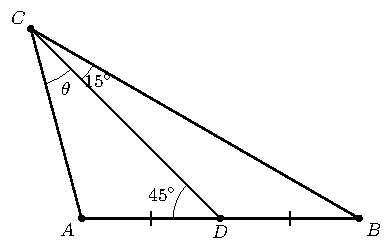
\includegraphics[
                width=0.52\textwidth
            ]{Figures/PastProblems/Problem2024.3/ProblemFigure.pdf}
        \end{center}
    \end{pastproblem}

    \begin{solutions}
        \begin{solution}
            Let $E$ be the foot of the perpendicular from $C$ to the line $AB$.
            Since $A,D,B$ are collinear and $\angle ADC=45^\circ$, we have
            \[
                \angle CDE=45^\circ.
            \]
            Thus $\triangle CED$ is a $45^\circ$--$45^\circ$--$90^\circ$ triangle.
            Set
            \[
                CE=\ell.
            \]
            Then
            \[
                ED=\ell.
            \]

            Also,
            \[
                \angle BDC
                =
                180^\circ-\angle ADC
                =
                135^\circ,
            \]
            so in $\triangle BCD$,
            \[
                \angle CBD
                =
                180^\circ-135^\circ-15^\circ
                =
                30^\circ.
            \]
            Hence $\triangle CEB$ is a $30^\circ$--$60^\circ$--$90^\circ$ triangle, and therefore
            \[
                EB=\sqrt{3}\,\ell.
            \]
            The equality $\angle CDE=45^\circ$ places $E$ on the $A$-side of $D$,
            so $D$ lies between $E$ and $B$. Hence
            \[
                DB
                =
                EB-ED
                =
                (\sqrt{3}-1)\ell.
            \]
            Because $D$ is the midpoint of $\overline{AB}$,
            \[
                AD=DB=(\sqrt{3}-1)\ell.
            \]
            In particular $AD<ED$, so the points occur in the order $E,A,D,B$, and
            \[
                EA
                =
                ED-AD
                =
                (2-\sqrt{3})\ell.
            \]

            Since $\angle ECD=45^\circ$ and $\angle ACD=\theta$,
            \[
                \angle ECA=45^\circ-\theta.
            \]
            Applying the tangent ratio in the right triangle $CEA$ gives
            \[
                \tan(45^\circ-\theta)
                =
                \frac{EA}{CE}
                =
                2-\sqrt{3}.
            \]
            On the other hand, the tangent subtraction formula gives
            \[
                \tan 15^\circ
                =
                \tan(45^\circ-30^\circ)
                =
                \frac{1-1/\sqrt{3}}{1+1/\sqrt{3}}
                =
                2-\sqrt{3}.
            \]
            Since $0^\circ<45^\circ-\theta<45^\circ$, we conclude that
            \[
                \boxed{\theta=30^\circ}.
            \]
        \end{solution}

        \begin{solution}
        Since $A,D,B$ are collinear,
        \[
            \angle BDC
            =
            180^\circ-\angle ADC
            =
            135^\circ.
        \]
        Therefore, in $\triangle BCD$,
        \[
            \angle CBD
            =
            180^\circ-135^\circ-15^\circ
            =
            30^\circ.
        \]
        By the Sine Rule,
        \[
            \frac{DB}{CD}
            =
            \frac{\sin 15^\circ}{\sin 30^\circ}
            =
            2\sin 15^\circ.
        \]

        Let $\theta=\angle ACD$. In $\triangle ACD$,
        \[
            \angle CAD
            =
            180^\circ-45^\circ-\theta
            =
            135^\circ-\theta.
        \]
        Again by the Sine Rule,
        \[
            \frac{AD}{CD}
            =
            \frac{\sin\theta}{\sin(135^\circ-\theta)}.
        \]
        Since $AD=DB$, we obtain
        \[
            \frac{\sin\theta}{\sin(135^\circ-\theta)}
            =
            2\sin 15^\circ.
        \]
        Expanding the denominator gives
        \[
            \sin\theta
            =
            \sqrt{2}\sin 15^\circ
            (\sin\theta+\cos\theta).
        \]
        Since
        \[
            \sqrt{2}\sin 15^\circ
            =
            \frac{\sqrt{3}-1}{2},
        \]
        it follows that
        \[
            \tan\theta
            =
            \frac{1}{\sqrt{3}}.
        \]
        As $\theta$ is an interior angle of the triangle, we conclude that
        \[
            \boxed{\theta=30^\circ}.
        \]
        \end{solution}
    \end{solutions}

    \begin{pastproblem}{2024.4}
        Let $C$ be a convex subset of $\R^3$. Here convex means that for any two points
        $\mathbf{p},\mathbf{q}\in C$, the line segment joining $\mathbf{p}$ and $\mathbf{q}$ is also
        contained in $C$.

        Suppose that the following two facts are known:
        \begin{problemchoices}
            \item The intersection of $C$ with the $xy$-plane is
                  \[
                      C\cap\{z=0\}
                      =
                      \{(x,y,0)\mid x^2+4y^2\leq 1\}.
                  \]
            \item The set $C$ contains the $z$-axis.
        \end{problemchoices}
        Determine the volume of $C$ in the region $-1\leq z\leq 1$, or determine that the given
        information is insufficient.
        \begin{problemchoices}
            \item This cannot be determined.
            \item $\pi$
            \item $2\pi$
            \item $4\pi$
        \end{problemchoices}
    \end{pastproblem}

    \begin{solution}
        Let
        \[
            E=\{(x,y)\in\R^2\mid x^2+4y^2\leq 1\}.
        \]
        By condition (1),
        \[
            C\cap\{z=0\}=E\times\{0\}.
        \]
        The ellipse $E$ has semiaxes $1$ and $\dfrac{1}{2}$, so its area is
        \[
            \area(E)
            =
            \pi\cdot 1\cdot \frac{1}{2}
            =
            \frac{\pi}{2}.
        \]

        For each height $z$, define the horizontal cross-section
        \[
            C_z
            =
            \{(x,y)\in\R^2\mid (x,y,z)\in C\}.
        \]
        By Cavalieri's principle (Theorem~\ref{pp:cavalieri}), the volume is determined by these cross-sectional areas. We will show that every $C_z$ contains the interior of $E$ and is contained in $E$. Possible differences on the ellipse boundary do not affect area.

        First, we show that $C_z\subseteq E$. Suppose that $(x,y,z)\in C$ and
        \[
            x^2+4y^2>1.
        \]
        Since $C$ contains the $z$-axis, the point $(0,0,t)$ belongs to $C$ for every $t\in\R$. By
        convexity, the line segment joining $(x,y,z)$ and $(0,0,t)$ is contained in $C$.

        For any $\alpha\in(0,1)$, we may choose
        \[
            t=-\frac{\alpha z}{1-\alpha}
        \]
        so that this segment intersects the $xy$-plane at the point
        \[
            (\alpha x,\alpha y,0).
        \]
        Since $\alpha$ can be chosen sufficiently close to $1$, we may arrange that
        \[
            (\alpha x)^2+4(\alpha y)^2>1.
        \]
        This would give a point of $C\cap\{z=0\}$ lying outside $E\times\{0\}$, contradicting
        condition (1). Therefore,
        \[
            C_z\subseteq E
        \]
        for every $z$.

        Conversely, we show that the interior of $E$ is contained in every $C_z$. Take $(x,y)$ with
        \[
            x^2+4y^2<1.
        \]
        Choose $\alpha\in(0,1)$ sufficiently close to $1$ so that
        \[
            \left(\frac{x}{\alpha}\right)^2
            +
            4\left(\frac{y}{\alpha}\right)^2
            \leq 1.
        \]
        Then
        \[
            \left(\frac{x}{\alpha},\frac{y}{\alpha},0\right)\in C.
        \]
        Also, since $C$ contains the $z$-axis,
        \[
            \left(0,0,\frac{z}{1-\alpha}\right)\in C.
        \]
        By convexity, their convex combination also belongs to $C$, and
        \[
            \alpha
            \left(\frac{x}{\alpha},\frac{y}{\alpha},0\right)
            +
            (1-\alpha)
            \left(0,0,\frac{z}{1-\alpha}\right)
            =
            (x,y,z).
        \]
        Hence $(x,y)\in C_z$.

        Thus, for every $z$,
        \[
            E^\circ\subseteq C_z\subseteq E.
        \]
        Since the boundary of the ellipse has area $0$, we have
        \[
            \area(C_z)=\area(E)=\frac{\pi}{2}
        \]
        for every $z$. Therefore, the volume of $C$ in the region $-1\leq z\leq 1$ is
        \[
            \int_{-1}^{1}\area(C_z)\dd z
            =
            \int_{-1}^{1}\frac{\pi}{2}\dd z
            =
            \pi.
        \]

        Therefore, the answer is $\boxed{(2)\ \pi}$.
    \end{solution}

    \begin{pastproblem}{2025.1}
        A fair coin is tossed repeatedly until either two heads in a row or two tails in a row
        appear. Determine the expected number of tosses before the process stops.
    \end{pastproblem}

    \begin{solution}
The first toss cannot stop the process. After any non-stopping history,
        the next toss matches the previous outcome with probability $1/2$.
        Let $G$ count the additional tosses, including the matching toss.
        For $k\in\N$, surviving $k-1$ additional tosses and then stopping gives
        \[
            \Prob(G=k)=\left(\frac12\right)^{k-1}\frac12.
        \]
        Thus $G\sim\Geom(1/2)$ under the convention in the distribution table:
        the successful trial is counted. Since $\Exp[G]=1/(1/2)=2$,
        the expected total number of tosses is
        \[
            1+\Exp[G]=\boxed{3}.
        \]
    \end{solution}

    \begin{pastproblem}{2025.2}
        The nineteenth-century mathematicians Cauchy and Weierstrass established rigorous
        definitions of limits. Identify the first mathematician to prove that the sum of the
        reciprocals of the squares of all positive integers is
        \[
            \sum_{n=1}^{\infty}\frac{1}{n^2}
            =
            \frac{\pi^2}{6}.
        \]
        \begin{problemchoices}
            \item David Hilbert
            \item Georg Cantor
            \item Bernhard Riemann
            \item Leonhard Euler
        \end{problemchoices}
    \end{pastproblem}

    \begin{solution}
        The problem of finding the exact value of the infinite series
        \[
            \sum_{n=1}^{\infty}\frac{1}{n^2}
        \]
        is known as the Basel problem.

        This problem had been known since the seventeenth century, and it was Leonhard Euler who
        first found and proved the famous identity
        \[
            \sum_{n=1}^{\infty}\frac{1}{n^2}
            =
            \frac{\pi^2}{6}.
        \]
        Therefore, the answer is $\boxed{(4)\ \text{Leonhard Euler}}$.
    \end{solution}

    \begin{pastproblem}{2025.3}
        Find the equation of the smallest sphere tangent to all four planes
        \[
            x=0,\qquad y=0,\qquad z=0,\qquad x+y+z=3.
        \]
    \end{pastproblem}

    \begin{solution}
        If a sphere of radius $r>0$ is tangent to the three coordinate planes,
        its center has the form
        \[
            \mathbf{c}=(\sigma_1r,\sigma_2r,\sigma_3r)^{\mathsf T},
            \qquad
            \sigma_1,\sigma_2,\sigma_3\in\{-1,1\}.
        \]
        Put $k=\sigma_1+\sigma_2+\sigma_3$, so
        \[
            k\in\{-3,-1,1,3\}.
        \]
        By the point-to-plane distance formula (Formula~\ref{pp:plane}), tangency to $x+y+z=3$ requires
        \[
            \frac{|kr-3|}{\sqrt3}=r.
        \]

        For $k=3$, the positive solutions are
        \[
            r=\frac{3}{3+\sqrt3}
            \qquad\text{and}\qquad
            r=\frac{3}{3-\sqrt3}.
        \]
        For $k=1$, the only positive solution is
        \[
            r=\frac{3}{1+\sqrt3},
        \]
        and for $k=-1$, the only positive solution is
        \[
            r=\frac{3}{\sqrt3-1}.
        \]
        The case $k=-3$ has no positive solution. Therefore the smallest
        radius is
        \[
            r=\frac{3}{3+\sqrt3}
            =\frac{3-\sqrt3}{2},
        \]
        attained when $\sigma_1=\sigma_2=\sigma_3=1$. Hence the center is
        \[
            \mathbf{c}
            =
            \left(
                \frac{3-\sqrt3}{2},
                \frac{3-\sqrt3}{2},
                \frac{3-\sqrt3}{2}
            \right)^{\mathsf T},
        \]
        and the required sphere is
        \[
            \boxed{
            \left(x-\frac{3-\sqrt3}{2}\right)^2
            +
            \left(y-\frac{3-\sqrt3}{2}\right)^2
            +
            \left(z-\frac{3-\sqrt3}{2}\right)^2
            =
            \left(\frac{3-\sqrt3}{2}\right)^2
            }.
        \]
    \end{solution}

    \begin{pastproblem}{2025.4}
        There are $200$ cards numbered from $1$ to $200$, all initially facing up. For each integer
        from $1$ to $200$, we call out that integer and flip every card whose number is a multiple
        of it. Determine the number of cards facing up after all $200$ calls.
        \begin{problemchoices}
            \item 142
            \item 153
            \item 164
            \item 175
            \item 186
        \end{problemchoices}
    \end{pastproblem}

    \begin{solution}
        A card numbered $n$ is flipped once for each positive divisor of $n$. Hence it is flipped
        $\tau(n)$ times, where $\tau(n)$ is the number of positive divisors of $n$.

        Divisors pair as $d$ and $n/d$; the only unpaired divisor occurs when $d=\sqrt n$. Thus $\tau(n)$ is odd if and only if $n$ is a perfect square. Therefore, exactly the cards numbered
        \[
            1^2,\quad 2^2,\quad 3^2,\quad \ldots,\quad 14^2
        \]
        are flipped an odd number of times, since
        \[
            14^2=196\leq 200<225=15^2.
        \]
        These $14$ cards end up facing down. The remaining
        \[
            200-14=186
        \]
        cards are facing up.

        Therefore, the answer is $\boxed{(5)\ 186}$.
    \end{solution}

    \begin{pastproblem}{2025.5}
        Determine which of $11^9$ and $9^{11}$ is larger.
    \end{pastproblem}

    \begin{solution}
        Taking logarithms, it is enough to compare
        \[
            9\ln 11
            \qquad\text{and}\qquad
            11\ln 9.
        \]
        Equivalently, compare
        \[
            \frac{\ln 11}{11}
            \qquad\text{and}\qquad
            \frac{\ln 9}{9}.
        \]
        The comparison-of-powers method uses $f(x)=\ln x/x$. Since $f'(x)=(1-\ln x)/x^2<0$ for $x>e$, this function is decreasing there. Since $9<11$ and both are greater than
        $e$, we have
        \[
            \frac{\ln 9}{9}
            >
            \frac{\ln 11}{11}.
        \]
        Hence
        \[
            11\ln 9>9\ln 11,
        \]
        so
        \[
            9^{11}>11^9.
        \]
        Therefore, the larger number is $\boxed{9^{11}}$.
    \end{solution}

    \begin{pastproblem}{2025.6}
        Roll a fair six-sided die repeatedly until a $6$ appears. Determine the expected sum of all
        rolls, including the final $6$.
    \end{pastproblem}

    \begin{solution}
        If $N$ is the stopping time, then $N\sim\Geom(1/6)$ and $\Exp[N]=6$. The total sum is at most $6N$, so its expectation is finite. Let $E$ be the desired expected sum. On the first roll, if the result is $6$, the process
        stops and contributes $6$. If the result is one of $1,2,3,4,5$, then the process returns to
        the same situation after contributing that roll.

        Therefore,
        \[
            E
            =
            \frac16\cdot 6
            +
            \frac16\sum_{k=1}^{5}(k+E).
        \]
        Hence
        \[
            E
            =
            1+\frac{15+5E}{6}
            =
            \frac72+\frac56E.
        \]
        Thus
        \[
            \frac16E=\frac72,
            \qquad
            E=21.
        \]
        Therefore, the answer is $\boxed{21}$.
    \end{solution}

    \begin{pastproblem}{2025.7}
        Determine the probability that at least two people in a group of $10$ share the same
        birthday. Assume a $365$-day year and that each day is equally likely.
    \end{pastproblem}

    \begin{solution}
        Under the standard independent-birthday model, use the complement as in Formula~\ref{pp:birthday}. It is easier to compute the probability that all $10$ birthdays are distinct.
        The first person may have any birthday, the second must avoid that birthday, the third must
        avoid the first two birthdays, and so on. Hence
        \[
            \Prob(\text{all birthdays are distinct})
            =
            \frac{365}{365}\cdot\frac{364}{365}\cdot\frac{363}{365}\cdots\frac{356}{365}.
        \]
        Therefore,
        \[
            \Prob(\text{at least two people share a birthday})
            =
            1-\frac{365}{365}\cdot\frac{364}{365}\cdot\frac{363}{365}\cdots\frac{356}{365}.
        \]
        Therefore, the answer is
        \[
            \boxed{1-\frac{364}{365}\cdot\frac{363}{365}\cdots\frac{356}{365}}.
        \]
    \end{solution}

    \begin{pastproblem}{2025.8}
        Find the largest of the following numbers:
        \begin{problemchoices}
            \item \(e^\pi\)
            \item \(\pi^e\)
            \item \(\sqrt{500}\)
            \item $7\pi$
        \end{problemchoices}
    \end{pastproblem}

    \begin{solution}
        Using the mathematical constants listed at the beginning of the book gives
        \[
            e^\pi \approx 23.14,
            \qquad
            \pi^e \approx 22.46,
            \qquad
            \sqrt{500} \approx 22.36,
            \qquad
            7\pi \approx 21.99.
        \]
        Therefore, the answer is $\boxed{(1)\ e^\pi}$.
    \end{solution}

    \begin{pastproblem}{2025.9}
        There are three doors. One hides a car and the other two hide goats.
        After the contestant chooses a door, a host who knows the car's location
        must open an unchosen door hiding a goat; when two such doors are
        available, the host follows a rule independent of the car's location.
        The contestant may then keep the original choice or switch to the only
        other unopened door. Determine which choice gives the higher probability
        of winning the car.
        \begin{problemchoices}
            \item The probabilities are the same.
            \item It is better not to switch.
            \item It cannot be determined.
            \item It is better to switch.
        \end{problemchoices}
    \end{pastproblem}

    \begin{solution}
        The original choice contains the car with probability $1/3$ and is
        wrong with probability $2/3$. Under the stated host protocol, switching
        wins exactly when the original choice was wrong. Hence staying wins with
        probability $1/3$, whereas switching wins with probability $2/3$.

        Therefore, the answer is
        \[
            \boxed{(4)\ \text{It is better to switch}}.
        \]
    \end{solution}

    \begin{pastproblem}{2025.10}
        Determine which of the following Fields Medalists majored in history rather than mathematics
        as an undergraduate.
        \begin{problemchoices}
            \item June Huh
            \item Caucher Birkar
            \item Edward Witten
            \item Simon Donaldson
            \item William Thurston
        \end{problemchoices}
    \end{pastproblem}

    \begin{solution}
        Edward Witten is famous as a mathematical physicist and was the first physicist to receive
        the Fields Medal. As an undergraduate, he majored in history rather than mathematics.

        Therefore, the answer is $\boxed{(3)\ \text{Edward Witten}}$.
    \end{solution}

    \begin{pastproblem}{2025.11}
        Determine which of the following mathematicians was not alive during the twentieth century.
        \begin{problemchoices}
            \item Sophus Lie
            \item Wilhelm Killing
            \item Alfred Young
            \item Hans Fitting
            \item Botong Wang
        \end{problemchoices}
    \end{pastproblem}

    \begin{solution}
        Sophus Lie lived from $1842$ to $1899$, so he died before the twentieth century began. The
        other listed mathematicians were alive at some point during the twentieth century.

        Therefore, the answer is $\boxed{(1)\ \text{Sophus Lie}}$.
    \end{solution}

    \begin{pastproblem}{2025.12}
        K\"onigsberg was the capital of East Prussia and a major center of European scholarship for
        many years. It was also the hometown of Immanuel Kant, David Hilbert, and J\"urgen Moser.
        The famous Seven Bridges of K\"onigsberg problem, in which Leonhard Euler proved that no
        solution exists, marked the beginning of both topology and graph theory. Determine the
        present-day country containing the former city of K\"onigsberg.
        \begin{problemchoices}
            \item Germany
            \item Poland
            \item Lithuania
            \item Russia
            \item Republic of Korea
        \end{problemchoices}
    \end{pastproblem}

    \begin{solution}
        The historical city K\"onigsberg is now Kaliningrad. Kaliningrad is a city in Russia.

        Therefore, the answer is $\boxed{(4)\ \text{Russia}}$.
    \end{solution}

    \begin{pastproblem}{2025.13}
        A fair coin is flipped $50$ times, and each outcome is recorded as either heads $(H)$ or
        tails $(T)$. A run is a maximal consecutive sequence of the same outcome. For example, if the
        result is
        $HHTTTH$, there are $3$ runs: $HH$, $TTT$, and $H$. Determine the expected number of runs.
        \begin{problemchoices}
            \item 24.5
            \item 25
            \item 25.5
            \item 26
        \end{problemchoices}
    \end{pastproblem}

    \begin{solution}
        The first toss always starts one run. For each position from the second toss onward, a new
        run begins exactly when the current toss differs from the previous toss.

        For a fair coin,
        \[
            \Prob(\text{current toss differs from previous toss})=\frac12.
        \]
        For $2\leq i\leq50$, let
        \[
            I_i
            =
            \indicator{\{\text{a new run starts at position }i\}}.
        \]
        The indicator $I_i$ is $1$ when a new run starts and $0$ otherwise. If $R$ denotes the total number of runs, then
        \[
            R=1+\sum_{i=2}^{50}I_i.
        \]
        Since $\Exp[I_i]=\Prob(I_i=1)=1/2$, linearity of expectation (Proposition~\ref{pp:linearity}) gives
        \[
            \Exp[R]
            =
            1+\sum_{i=2}^{50}\Exp[I_i]
            =
            1+49\cdot\frac12
            =
            25.5.
        \]
        Therefore, the answer is $\boxed{(3)\ 25.5}$.
    \end{solution}

    \begin{pastproblem}{2025.14}
        Determine which of the following results appeared first historically.
        \begin{problemchoices}
            \item Bayes' Theorem
            \item Intermediate Value Theorem
            \item Cauchy--Schwarz Inequality
            \item Fundamental Theorem of Calculus
        \end{problemchoices}
    \end{pastproblem}

    \begin{solution}
        Interpreting the question by the earliest recognizable form of each
        result, the inverse relationship between differentiation and integration
        was established in seventeenth-century work associated with Barrow,
        Newton, and Leibniz. Bayes' theorem was published in the eighteenth
        century, while rigorous forms of the Intermediate Value Theorem and the
        Cauchy--Schwarz inequality appeared in the nineteenth century.

        Therefore, the intended answer is
        \[
            \boxed{(4)\ \text{Fundamental Theorem of Calculus}}.
        \]
    \end{solution}

    \begin{pastproblem}{2025.15}
        Which of the following amounts is closest to the Abel Prize money?
        \begin{problemchoices}
            \item None
            \item About \$1{,}000{,}000
            \item About \$1{,}500{,}000
            \item About \$2{,}000{,}000
        \end{problemchoices}
    \end{pastproblem}

    \begin{solution}
        In 2025, the Abel Prize amounted to NOK $7.5$ million. Using the exchange rate relevant at
        the time, this was closest to one million US dollars among the listed choices.

        Therefore, the answer is $\boxed{(2)\ \text{About }\$1{,}000{,}000}$.
    \end{solution}

    \begin{pastproblem}{2025.16}
        Determine which of the following mathematicians has received both the Fields Medal and the
        Abel Prize.
        \begin{problemchoices}
            \item John Milnor
            \item Terence Tao
            \item June Huh
            \item No one
        \end{problemchoices}
    \end{pastproblem}

    \begin{solution}
        John Milnor received the Fields Medal in $1962$ and the Abel Prize in $2011$. Therefore he
        has received both prizes.

        Therefore, the answer is $\boxed{(1)\ \text{John Milnor}}$.
    \end{solution}

    \begin{pastproblem}{2025.17}
        A fair six-sided die is rolled until all $6$ faces have appeared. Determine the probability
        that no odd-numbered face appears before all even-numbered faces have appeared.
        \begin{problemchoices}
            \item \(20\%\)
            \item \(15\%\)
            \item \(10\%\)
            \item \(5\%\)
        \end{problemchoices}
    \end{pastproblem}

    \begin{solution}
        Ignore repeated rolls and look only at the order in which new faces appear. The condition is
        that the first three distinct faces to appear are exactly the even faces $2,4,6$ in some
        order.

        The probability that the first new face is even is $3/6$. Given that one even face has
        appeared, the probability that the next new face is also even is $2/5$. Given that two even
        faces have appeared, the probability that the next new face is the remaining even face is
        $1/4$. Therefore the desired probability is
        \[
            \frac36\cdot\frac25\cdot\frac14
            =
            \frac1{20}
            =
            5\%.
        \]
        Therefore, the answer is $\boxed{(4)\ 5\%}$.
    \end{solution}

    \begin{pastproblem}{2025.18}
        In the Tower of Hanoi puzzle, $5$ disks are stacked on peg $A$ from largest to smallest.
        The objective is to move all disks to peg $C$ using auxiliary peg $B$, subject to the
        following rules:
        \begin{problemchoices}
            \item Only one disk may be moved at a time.
            \item A larger disk may not be placed on a smaller disk.
            \item Peg $B$ may be used freely.
        \end{problemchoices}
        Determine the minimum number of moves required.
        \begin{problemchoices}
            \item 25
            \item 31
            \item 32
            \item 63
            \item 120
        \end{problemchoices}
    \end{pastproblem}

    \begin{solution}
        Let $T(n)$ be the minimum number of moves needed for $n$ disks. To move $n$ disks, first
        move the top $n-1$ disks to the auxiliary peg, then move the largest disk once, and finally
        move the $n-1$ disks onto the largest disk. These two transfers are also necessary before and after the largest disk reaches its destination, so the construction attains the lower bound. Hence
        \[
            T(n)=2T(n-1)+1,
            \qquad
            T(1)=1.
        \]
        This is the Tower of Hanoi recurrence in Formula~\ref{pp:hanoi}; solving it gives
        \[
            T(n)=2^n-1.
        \]
        Therefore,
        \[
            T(5)=2^5-1=31.
        \]
        Therefore, the answer is $\boxed{(2)\ 31}$.
    \end{solution}

    \begin{pastproblem}{2025.19}
        Determine the last two digits of $7^{123}$, expressed as a two-digit number.
        \begin{problemchoices}
            \item 37
            \item 41
            \item 43
            \item 49
        \end{problemchoices}
    \end{pastproblem}

    \begin{solution}
        Work modulo $100$. Since
        \[
            7^4=2401\equiv 1\pmod{100},
        \]
        and
        \[
            123=4\cdot 30+3,
        \]
        we have
        \[
            7^{123}
            =
            (7^4)^{30}7^3
            \equiv
            1^{30}\cdot 343
            \equiv
            43
            \pmod{100}.
        \]
        Therefore, the answer is $\boxed{(3)\ 43}$.
    \end{solution}

\end{document}
